
\frontmatter
\title{MCTest:\\
Como Criar e Corrigir Exames Parametrizados Automaticamente}
\author{Francisco de Assis Zampirolli}
% \author{Francisco de Assis Zampirolli \\
% João Marcelo Borovina Josko \\
% Paulo Henrique Pisani}

\date{\today}
%\date{7 de setembro de 2023}


\maketitle
% ---
% Ficha Catalográfica
% ---
% Isto é um exemplo de Ficha Catalográfica, ou ``Dados internacionais de
% catalogação-na-publicação''. Você pode utilizar este modelo como referência. 
% Porém, talvez a biblioteca lhe fornece um PDF
% com a ficha catalográfica definitiva após a defesa do trabalho. Quando estiver
% com o documento, salve-o como PDF no diretório do seu projeto e substitua todo
% o conteúdo de implementação deste arquivo pelo comando abaixo:
%
% \begin{fichacatalografica}
%     \includepdf{fig_ficha_catalografica.pdf}
% \end{fichacatalografica}

\textcopyright\ 2024 Francisco de Assis Zampirolli da Universidade Federal do ABC (UFABC). 

Todos os direitos reservados. \\ \\

Este livro está sob a Licença: 

\hspace{1cm}\textit{Creative Commons
Attribution-ShareAlike 4.0 International License}

\hspace{1cm}Detalhes no endereço: \href{https://creativecommons.org/licenses/by-sa/4.0}{creativecommons.org/licenses/by-sa/4.0}\\ \\


\textbf{Projeto gráfico:} Francisco de Assis Zampirolli \\

\begin{verse}
	\vspace*{\fill}					% Posição vertical

	\begin{center}					% Minipage Centralizado

\hrule							% Linha horizontal
\vspace{1cm}
CATALOGAÇÃO NA FONTE

SISTEMA DE BIBLIOTECAS DA UNIVERSIDADE FEDERAL DO ABC

 \vspace{5mm}

 \fbox{%
 \hspace{5mm}
\parbox{0.92\linewidth}{%
	\begin{minipage}[c]{13cm}		% Largura


 \vspace{5mm}


    \noindent
Z26m  Zampirolli, Francisco de Assis

	\hspace{0.5cm} MCTest : como criar e corrigir exames parametrizados automaticamente / Francisco de Assis Zampirolli -- Santo André, SP : Edição do Autor, 2024. \\
	
	\hspace{0.5cm} xxiv, 244 p. : il.\\
	
	\hspace{0.5cm}  ISBN: 978-65-00-79086-3 (1a Edição)\\
	
	\hspace{0.5cm}
        1. Avaliação da Aprendizagem.
        2. Correção Automática.
        3. Questão Paramétrica.
        4. Programação -- Problemas e Exercícios.
        5. Moodle. Título. \\ 			
	
	\hfill CDD 22 ed. –- 005.4\\
  
	\end{minipage}
   }%
   }%
 \\
 %Elaborado por Marciléia Ap. de Paula -- CRB-8/8530

 \end{center}

\end{verse}
\vspace{3cm}
% ---\cleardoublepage
% ---
% Dedicatória
% ---
\begin{verse}
   \vspace*{\fill}
   \centering
   \noindent
   \textit{
Dedico este trabalho com imenso amor à minha esposa Cristina e aos meus filhos, Rafael e Eduardo. Agradeço de coração por estarem sempre ao meu lado em todas as conquistas e desafios da vida. 
} \vspace*{\fill}
\end{verse}
% ---\cleardoublepage
%% ---
% Agradecimentos
% ---
\chapter*{Agradecimentos}

Agradeço em primeiro lugar aos meus pais, que mesmo sendo lavradores, filhos de imigrantes italianos e não conhecendo o significado de um mestrado ou doutorado, me ensinaram a importância do estudo e da dedicação ao trabalho a ser realizado.

Apesar de não ter contato com muitos colegas e professores da UFES, eles foram fundamentais na motivação para uma vida acadêmica. Em especial aos excelentes profs. Francisco Jose Negreiros Gomes e Ricardo de Almeida Falbo, que nos deixaram, tão novos!

Aos colegas e professores do IME/USP, com os quais tive uma imersão profunda aos estudos avançados em computação, com um degrau elevado a ser transposto, mas superado, com a ajuda de amigos e do  orientador, prof. Junior Barrera, também na orientação para estender a biblioteca \texttt{MMach} para grafos. No IME tive a honra de ter aulas com os pioneiros da computação no Brasil, como os profs. Imre Simon, Siang Wun Song e Valdemar Setzer. Além disso, em uma cidade vibrante como São Paulo, foi possível vivenciar um grande desenvolvimento cultural, juntamente com amigos do IME: Alexandre Bizetti e Fabio Henrique Viduani Martinez (esses também do apto 209-G do CRUSP), Claus Akira Matsushigue, Jair Donadelli Júnior, Luiz Carlos da Silva Rozante, Marcelo de Souza Lauretto, Marco Aurélio Stefani, e vários outros.

Aos colegas e professores da FEEC/UNICAMP, em especial o orientador prof. Roberto de Alencar Lotufo, pela objetividade em concluir o doutorado, além da orientação no desenvolvimento da documentação da biblioteca \texttt{mmorph}.

Aos colegas, alunos e professores dos Centros Universitários Senac e Fei, com os quais consegui adquirir experiências importantes como docente em cursos de computação.

Agradeço aos colegas da UFABC, professores, técnicos e alunos, que foram fundamentais para chegar até esse pedido de promoção para professor titular do magistério superior, título desejado há muito tempo. São vários os colegas, alguns apontados nos trabalhos colaborativos citados neste memorial. Mas não poderia deixar de nomear: 
Carla Lopes Rodriguez,
Carlos da Silva dos Santos,
Denise Hideko Goya,
Edson Alex Arrazola Iriarte,
Edson Pinheiro Pimentel,
Fernando Teubl Ferreira,
Guiou Kobayashi,
Jair Donadelli Júnior,
João Marcelo Borovina Josko,
José Artur Quilici-Gonzalez, 
Juliana Cristina Braga,
Luiz Carlos da Silva Rozante,
Paulo Henrique Pisani,
Rogério Perino de Oliveira Neves,
Valério Ramos Batista, e
Wagner Tanaka Botelho.

Expresso aqui a minha gratidão a todos que, de forma direta ou indireta, contribuíram para a minha jornada acadêmica. Sou imensamente grato pela ajuda e apoio oferecidos ao longo desse percurso.

%% ---\cleardoublepage
\chapter*{Epígrafe}\normalsize

\begin{verse}
    \vspace*{\fill}
	\begin{flushright}
		\textit{``Não basta saber, é preciso aplicar. Não basta querer, é preciso também fazer.''\\
		          (Johann Wolfgang von Goethe)}
	\end{flushright}
\end{verse}
\cleardoublepage
\chapter*{Prefáceis}\normalsize

\section*{Prefácio da primeira edição}

% CONTEXTO
A avaliação dos estudantes é uma atividade crucial para o trabalho de um professor, ao permitir avaliar de maneira precisa o desempenho dos estudantes ao longo do curso, fornecendo \textit{feedback} importante para o seu desenvolvimento acadêmico. Além disso, a avaliação também é um meio importante para aprimorar a prática educativa, permitindo que os professores identifiquem pontos fortes e fracos de sua metodologia e aprimorem sua abordagem pedagógica para proporcionar um melhor aprendizado aos estudantes.

% LACUNA
Avaliar inúmeros estudantes individualizadamente é uma tarefa desafiadora para professores em todos os níveis de ensino, especialmente em disciplinas que exigem habilidades e competências específicas. Esse desafio é ainda maior em exames que envolvem exercícios de programação (EP), uma vez que exigem uma avaliação minuciosa dos processos de resolução de problemas, além da compreensão do código e da lógica utilizados pelos estudantes.

% PROPÓSITO
Este livro visa prover uma solução abrangente e eficaz para a avaliação de estudantes. A abordagem colaborativa adotada por docentes da Universidade Federal do ABC (UFABC), empregando o sistema de código aberto MCTest, viabiliza a reutilização de conjuntos de questões previamente utilizados por outros colegas que ministram a mesma disciplina.

% MÉTODO
O  MCTest permite a criação e correção de exames de múltipla escolha e dissertativa, incluindo EP no \textit{plugin} VPL (\href{https://vpl.dis.ulpgc.es}{ \textit{Virtual Programming Lab}}) do ambiente Moodle. Ele oferece questões parametrizadas e exames individualizados que podem ser usados por várias turmas simultaneamente. A principal contribuição desse sistema reside na capacidade de compartilhar questões parametrizadas, que incorporam enunciados em \LaTeX{} intercalados com códigos em Python. 

% RESULTADOS
Este livro consolida mais de uma década de experiência na avaliação anual de milhares de estudantes, a partir de 2012, quando se deu início à automatização do processo seletivo da Especialização em Tecnologias e Sistemas de Informação (TSI) da UFABC, com a criação da primeira versão do MCTest, desenvolvida em Matlab. Desde então, o sistema passou por um substancial processo de evolução, beneficiando-se da colaboração de diversos colegas da UFABC, cujas contribuições permitiram identificar novas necessidades e aprimorar suas funcionalidades. A versão web mais recente abordada neste livro é a 5.2 e encontrando-se disponível para instalação no endereço \href{https://github.com/fzampirolli/mctest}{github.com/fzampirolli/mctest}. Duas implantações ativas do sistema estão em execução na UFABC: a versão de produção, hospedada em \href{http://mctest.ufabc.edu.br}{mctest.ufabc.edu.br}; e a versão de desenvolvimento, \textit{backup} e divulgação em \href{http://vision.ufabc.edu.br}{vision.ufabc.edu.br}.

É de extrema importância enfatizar que o MCTest não tem um caráter comercial e não segue rigidamente o ciclo de vida convencional de desenvolvimento de software. Sua abordagem é fundamentada na prototipagem, seguindo os princípios da Engenharia de Software, em suma, novos requisitos e protótipo rápido para validação de conceitos. No entanto, até o momento, o sistema ainda não atingiu sua versão final, desenvolvido predominantemente por um único programador (com exceção da adaptação realizada no VPL, pelo Heitor Rodrigues Savegnago e seu orientador Prof. Dr. Paulo Henrique Pisani, a quem expresso minha sincera gratidão). Para poder progredir em direção a um produto comercial, seriam necessários processos de engenharia reversa e contínuos aprimoramentos. 

% uso na UFABC
Apesar das limitações acima mencionadas, o MCTest é utilizado por alguns docentes e gestores da UFABC, desempenhando um papel de significativa relevância no âmbito da avaliação discente. Essa utilização resulta não apenas em uma notável redução da carga de trabalho repetitivo, mas também contribui para a mitigação de possíveis ocorrências de falhas. 

% implantação
A implantação do sistema é agilizada por meio da adoção do ambiente \textit{VirtualBox} (\href{https://www.virtualbox.org}{virtualbox.org}), que permite uma implantação local para fins de teste em uma máquina com bom desempenho de processamento, armazenamento (5 GB livre) e memória RAM ($\geq$ 8 GB). Ao optar pela instalação dos sistemas operacionais Ubuntu ou Mint, seguida pela subsequente execução do arquivo \href{https://github.com/fzampirolli/mctest/blob/master/_setup-all.sh}{\_setup-all.sh} disponibilizado no repositório GitHub (\href{https://github.com/fzampirolli/mctest}{github.com/fzampirolli/mctest}), mediante privilégios de administrador, o MCTest é instalado de forma contínua, estando acompanhado por um conjunto inicial de dados de teste presente no arquivo \verb|mctest.sql|. Os exemplos ilustrativos apresentados neste trabalho encontram-se no arquivo \verb|book/1ed-br/mctestLivro.sql|, estando também acessíveis no repositório GitHub. A fim de empregar esses exemplos no MCTest, é necessário observar as instruções fornecidas no arquivo \href{https://github.com/fzampirolli/mctest/blob/master/_setup-all.sh}{\_setup-all.sh}.

A obra foi elaborada em 14 capítulos, divididos em quatro partes principais. A Parte \ref{part:fundamentos} tem como principal objetivo introduzir os leitores ao sistema, oferecendo detalhes sobre seus componentes e funcionalidades essenciais. A Parte \ref{part:questoesMCTest} explora a variedade de tipos de questões disponíveis. A Parte \ref{part:exames} abrange a criação e administração de exames. Por fim, a Parte \ref{part:experimentos} proporciona estudos de caso e exemplos práticos, sendo estes últimos divulgados em artigos científicos. Estes experimentos foram realizados em modalidades híbridas, totalmente remotas e totalmente presenciais. 
%
Para aqueles sem interesse na parte paramétrica, que requer conhecimentos de programação, ou sem usar o banco de questões, há a possibilidade de pular diversos capítulos, conforme explicado no final do Capítulo \ref{ch:introducao}.

% CONCLUSÃO
Ao usar o MCTest, os professores têm à disposição uma ferramenta para aprimorar a avaliação das habilidades e competências dos estudantes. Assim, os docentes conseguem reduzir o esforço exigido na criação e correção de exames e atividades práticas. No entanto, o ponto crucial desse processo reside na ampla coleção de questões elaboradas e disponibilizadas pelos professores da UFABC, que atualmente totalizam 2.273 questões, embora limitadas aos docentes de cada disciplina.

O MCTest permanece em constante processo de evolução e aprimoramento, incentivando os usuários a contribuírem com suas experiências para torná-lo ainda mais eficiente e alinhado com as demandas educacionais em constante transformação.

Ao longo desta obra, as funcionalidades do MCTest serão exploradas, permitindo aos leitores compreenderem suas características e recursos. Espera-se que esse trabalho proveja um guia completo sobre como empregar o MCTest em ambientes educacionais.

A partir de 2023, estudantes de Trabalho de Conclusão de Curso e Mestrado em Ciência da Computação na UFABC desempenham um papel ativo no processo de implementação de melhorias no sistema. Há expectativas de que essas melhorias sejam incorporadas à versão atual disponibilizada no GitHub. É importante ressaltar, contudo, que ainda existem áreas que demandam aprimoramento. Isso inclui a navegação entre as interfaces e a avaliação das competências e habilidades dos estudantes. Por exemplo, em um EP submetido por meio do VPL, quando se requer a utilização de estruturas de repetição com o comando \textit{while}, a avaliação deve ser condizente com o cumprimento ou descumprimento dessa especificação.

Com o intuito de aprimorar a compreensão durante a leitura, é importante salientar que os seguintes termos serão amplamente utilizados ao longo deste trabalho: exercício de programação (EP), questão de múltipla escolha (QM), questão dissertativa ou de texto (QT) e quadro de respostas (QR). Nesse contexto, os estudantes efetuam as marcações das QMs no QR.

Leitores interessados em adquirir versões impressas deste livro podem encontrar mais informações na pasta \verb|book| disponível no seguinte endereço:
\href{https://github.com/fzampirolli/mctest/tree/master/book/1ed-br}{github.com/fzampirolli/mctest}.

Este livro foi concebido e elaborado exclusivamente pelo autor. No entanto, lamentavelmente, não passou por um processo de revisão formal. Os textos apresentados foram predominantemente avaliados por meio de consultas a redes generativas, pertencentes a uma categoria de modelos de aprendizado de máquina. A compreensão dos colegas interessados é confiada para o aprimoramento de edições futuras por meio de seus valiosos \textit{feedbacks} construtivos.

Finalmente, é de suma importância enfatizar que as opiniões e declarações apresentadas nesta obra são devidamente embasadas por referências sempre que possível, ou por meio de experimentos realizados e devidamente citados no próprio livro. Nos casos em que a obtenção de referências se torna inviável, tais posicionamentos refletem a perspectiva pessoal do autor e não devem ser considerados uma representação oficial da instituição à qual o autor está afiliado.

\begin{verse}
    \vspace*{2mm}
	\begin{flushright}
		Francisco de Assis Zampirolli\\
            \date{7 de setembro de 2023}
	\end{flushright}
\end{verse}

\newpage

%%%%%%%%%%%%%%%%%%%%%%%%%%%%%%%%%%%%%%%%%%%%%%%%%%%%%%%%%%%%%%%%%%%%%%%%%%%%%%%%%%%%%%%%%%%%%%%%%%%

\section*{Prefácio da segunda edição -- em construção}

Aprimoramentos e correções realizados no texto da primeira edição deste livro \cite{Zampirolli2023:MCTest}, utilizando o MCTest versão 5.2, serão descritos nesta segunda edição e implementados na versão 5.3 do MCTest. No arquivo \href{https://github.com/fzampirolli/mctest/blob/master/_setup-all.sh}{\_setup-all.sh}, estão detalhadas as instruções para a instalação dessas versões. Agradeço aos colegas que destacaram informações não ressaltadas no texto original, as quais foram incorporadas nesta nova versão, conforme formato descrito a seguir:

\begin{mybox}{corEdicao2}{\textbf{Destaque:\\\vspace{-3mm}\hrule\vspace{3mm}}}
Este é um exemplo de destaque para chamar a atenção do leitor em algum ponto.
\end{mybox}

Na tela de atualização de questões, ver Seção \ref{sec:questaoQM} -- \nameref{sec:questaoQM}, foram adicionados cinco novos campos: contador de correções, contador de acertos e, para a Teoria de Resposta ao Item, os parâmetros \(a\)-discriminação, \(b\)-habilidade e \(c\)-chute. Esses parâmetros são fundamentais para a criação de exames adaptativos, ver Seção \ref{sec:testeAdaptativo} -- \nameref{sec:testeAdaptativo}. 

Nesta mesma tela de atualização de questões, o campo de ``Retorno desta alternativa'' (\textit{feedback}) foi alterado para também aceitar a parte paramétrica, entre \verb|[[code:| e \verb|]]|, já incluída em ``Descrição'' e ``Alternativas'' da questão.


A Seção \ref{sec:QMparametricaExtra} -- \nameref{sec:QMparametricaExtra} apresenta uma nova questão paramétrica altamente flexível, proporcionando uma extensa variedade de configurações e variações. Esta questão automatiza o processo de geração de itens, incorporando operadores relacionais e não relacionais, e oferece controle sobre parâmetros essenciais, como o número de itens, alternativas, operadores e itens corretos. Este tipo de questão, caracterizado por sua adaptabilidade através de parâmetros configuráveis, revela-se facilmente extensível para uma variedade de conjuntos, não se restringindo exclusivamente aos conjuntos de operadores relacionais e não relacionais. Para tal adaptação, é suficiente que o primeiro conjunto contenha elementos com premissas verdadeiras, enquanto o segundo apresente premissas falsas. Pode-se considerar, por exemplo, conjuntos como caracteres alfanuméricos permitidos em um nome de arquivo/variável versus caracteres proibidos, entre outros.


Na tela de atualizar exame, foi adicionado um novo campo para a seleção dos tópicos da disciplina que serão considerados na avaliação, ver Seção \ref{sec:exameTopicos} -- \nameref{sec:exameTopicos}. Após escolher o tópico desejado e clicar no botão ``Salvar'', apenas as questões relacionadas a esse tópico serão apresentadas. Este novo recurso é crucial para otimizar o tempo de carregamento da tela, especialmente em situações em que a disciplina possui inúmeras questões, resultando em uma melhoria significativa na eficiência do processo.

A opção pelo termo ``tela'' em detrimento de ``formulário'' é respaldada pela natureza das interfaces gráficas presentes no MCTest, as quais exibem informações provenientes de registros de tabelas de banco de dados. Em geral, essas páginas proporcionam uma visão mais abrangente dos atributos desses registros, enriquecendo a compreensão do conteúdo. Apesar da constante necessidade de aprimoramento na Interface Humano-Computador, a escolha por ``tela'' é orientada pela dinâmica e interatividade inerentes às informações apresentadas. Além disso, as figuras deste livro, que são representações visuais desses recortes de tela, buscam ilustrar a experiência do usuário, contribuindo para a compreensão e usabilidade do sistema.

Foi criada a Seção \ref{sec:testeAdaptativo} -- \nameref{sec:testeAdaptativo} para explicar o funcionamento de uma nova funcionalidade opcional que permite a criação de exames adaptativos, considerando o desempenho do estudante em exames anteriores. Para que essa funcionalidade opere corretamente, é necessário que as questões de múltipla escolha estejam classificadas conforme a taxonomia de Bloom e que sejam geradas várias variações do exame. Dessa forma, os estudantes que não obtiveram um bom desempenho em exames anteriores receberão exames personalizados, com níveis de questões classificados nos primeiros níveis dessa taxonomia.

No QRcode apresentado no PDF de um exame, foi incluída também a variação do exame, criada após clicar no botão ``Criar-Variações''. Esse recurso é importante para vincular o PDF digitalizado com as respostas dos estudantes à página do exame que será utilizada para fazer as correções, clicando no botão ``Upload-PDF''. Além disso, com essa informação no QRCode, não é mais necessário criar arquivo criptografado e compactado com o gabarito do exame, anteriormente armazenado no servidor. Agora, o gabarito de cada exame é acessado diretamente no banco de dados, na tabela contendo as variações do exame.

Foi inserida a Seção \ref{sec:recomendacoesCap8} -- \nameref{sec:recomendacoesCap8}, para destacar algumas recomendações essenciais para garantir a realização de um exame impresso com questões de múltipla escolha. Por exemplo, o método de correção automática \textbf{NÃO} funcionará se os quatro discos pretos não estiverem intactos na página digitalizada. Além disso, ao utilizar questões disponíveis no banco de dados do MCTest, é necessário clicar no botão ``Criar-Variações'' antes de clicar no botão ``Criar-PDF''. Adicionalmente, o número ID exibido ao lado do botão ``Criar-Variações'' \textbf{DEVE} ser o mesmo número exibido em vermelho na folha do exame impresso, abaixo do cabeçalho. Caso esses números difiram das páginas digitalizadas, a correção automática \textbf{NÃO} funcionará. O código foi adaptado para incluir a variação do exame também no QRCode. No entanto, para aceitar as variações anteriores, seria necessário armazenar todas as variações geradas no banco de dados, o que consumiria muito espaço em disco, sendo inviável no momento.

É altamente aconselhável seguir a prática de, antes de administrar um exame para uma ou diversas turmas com inúmeros estudantes, imprimir uma cópia, preenchê-la e submetê-la a uma correção automatizada. Caso essa abordagem demonstre eficácia durante essa simulação preliminar, é razoável esperar que funcione de maneira adequada durante a situação real de aplicação, correção e fornecimento de \textit{feedback} do exame.

Foi incluída na Seção \ref{sec:mctest+moodle+vpl+pdi} -- \nameref{sec:mctest+moodle+vpl+pdi} um resumo que descreve a implementação do MCTest-5 com Moodle+VPL no curso de Processamento Digital de Imagens (PDI). Enquanto os estudos anteriores abordaram cursos introdutórios de lógica de programação, este relato destaca a aplicação dessa integração em um contexto mais específico. O trabalho \textit{``A Practical Digital Image Processing Course with \texttt{morph.py}''} de \citeonline{2024:Zampirolli.Josko-PDI} foi premiado no Simpósio Brasileiro de Educação em Computação, consolidando uma jornada iniciada em 2012. Este curso prático utiliza a biblioteca Python \texttt{morph.py} para auxiliar no ensino de PDI, abordando conceitos desde o básico até avançado, apoiando-se em exemplos e exercícios práticos. Um estudo de caso com 15 participantes validou a eficácia do método, destacando os desafios e soluções encontrados no ensino de PDI para iniciantes.

O Apêndice \ref{ch:apendice} -- \nameref{ch:apendice} descreve uma experiência realizada na disciplina de Processamento da Informação na UFABC no primeiro quadrimestre de 2024, em duas turmas, com o objetivo de substituir a lista de presença por um processo automático de verificação de acesso dos estudantes no Moodle durante as aulas. Foi desenvolvido o serviço \texttt{LabMoodle}, que acompanha as atividades dos estudantes cadastrados em uma disciplina no Moodle. Além disso, foram oferecidos 80 Exercícios de Programação (EPs) com correção automática pelo VPL. A disciplina abordou os conceitos fundamentais de Lógica de Programação e foi ministrada em um laboratório de informática. A estratégia de ensino incluiu aulas conceituais no Google Colab seguidas da resolução dos EPs pelos estudantes, com ênfase em vetores e matrizes. Os resultados foram avaliados por meio de exames elaborados no MCTest e compostos por questões com correção automática utilizando o \textit{plugin} VPL do Moodle. O serviço \texttt{LabMoodle} permitiu o acompanhamento das atividades dos estudantes, destacando a participação e os acessos durante as aulas. Os dados coletados proporcionaram uma análise comparativa entre as duas turmas, evidenciando diferenças no desempenho e na participação dos estudantes antes e após a prova de recuperação. 

Finalmente, o Apêndice \ref{ch:apendiceB} -- \nameref{ch:apendiceB} continua o relato do apêndice anterior, porém focado nos testes adaptativos. Foram aplicados 6 testes, sendo apenas o primeiro não adaptativo. Esses testes foram utilizados como avaliação formativa com objetivo motivacional. Foram implementados 3 formas diferentes de criar esses testes adaptativos: SAT (\textit{Semi-Adaptive Testing}), WPC (\textit{Weighted Probability of Correctness}) e MLE (\textit{Maximum Likelihood Estimation}). A implementação desses testes foi realizada durante o andamento do curso, sendo o último MLE auxiliado pelo estudante Lucas Montagnani Calil Elias, como Trabalho de Conclusão de Curso do Bacharelado em Ciência da Computação na Universidade Federal do ABC. No final do curso, foi aplicado um questionário com 17 respondentes e realizada uma análise da significância estatística.


\begin{verse}
    \vspace*{2mm}
	\begin{flushright}
		Francisco de Assis Zampirolli\\
            \date{\today}
	\end{flushright}
\end{verse}
\cleardoublepage
%\chapter*{Resumo}\normalsize

% contexto
A avaliação dos estudantes é uma atividade crucial para o trabalho de um professor, ao permitir avaliar de maneira precisa o desempenho dos estudantes ao longo do curso, fornecendo \textit{feedback} importante para o seu desenvolvimento acadêmico. Além disso, a avaliação também é um meio importante para aprimorar a prática educativa, permitindo que os professores identifiquem pontos fortes e fracos de sua metodologia e aprimorem sua abordagem pedagógica para proporcionar um melhor aprendizado aos estudantes.
% lacuna
Avaliar inúmeros estudantes individualizadamente é uma tarefa desafiadora para professores em todos os níveis de ensino, especialmente em disciplinas que exigem habilidades e competências específicas. Esse desafio é ainda maior em exames que envolvem Exercícios de Programação (EP), uma vez que exigem uma avaliação minuciosa dos processos de resolução de problemas, além da compreensão do código e da lógica utilizados pelos estudantes. 
% objetivo
Este livro visa disponibilizar uma solução abrangente e eficaz para a avaliação de estudantes. A abordagem colaborativa adotada permite que os professores reutilizem bancos de questões já utilizados por outros colegas que lecionam na mesma disciplina, economizando tempo e esforço na criação de avaliações personalizadas.
% método
O sistema de código aberto MCTest permite a criação e correção de exames de múltipla escolha e dissertativa, incluindo EP. Ele oferece questões parametrizadas e exames individualizados que podem ser usados por várias turmas simultaneamente. O sistema foi inicialmente desenvolvido na Universidade Federal do ABC (UFABC) e evoluiu para uma versão web.
% resultados
O livro apresenta resultados de mais de uma década de experimentos em disciplinas da UFABC, realizados em modalidades híbridas, totalmente remotas e totalmente presenciais. Artigos e registros de software estão disponíveis para consulta detalhando esses experimentos, porém, são apresentados resumidamente neste livro.
% conclusão
Com a utilização do sistema MCTest apresentado neste livro, os professores têm à disposição uma ferramenta poderosa para aprimorar a avaliação das habilidades e competências dos estudantes. Ao adotar o MCTest, os professores podem reduzir significativamente o esforço necessário para criar e corrigir exames e atividades práticas, permitindo que se dediquem a atividades de ensino menos repetitivas e mais significativas, como aprimorar materiais didáticos e dedicar tempo para esclarecer dúvidas dos estudantes. Isso contribui para uma experiência educacional mais enriquecedora e eficiente, beneficiando tanto os docentes quanto os estudantes.\\ \vspace{5mm}

\noindent
 \textbf{Palavras-chave}: 
Avaliação individual.
Correção automática.
Questão paramétrica.
Exercício de programação.
Moodle.\cleardoublepage
\frontmatter

\setcounter{page}{11}
\tableofcontents\cleardoublepage
\listoffigures\cleardoublepage
\addcontentsline{toc}{chapter}{\listoflistingscaption}
\listoflistings
% Lista de abreviaturas e siglas

\chapter*{Lista de Abreviaturas e Siglas}\normalsize
\addcontentsline{toc}{chapter}{Lista de Abreviaturas e Siglas}

\begin{description}
  \item[ACM --] \textit{Association for Computing Machinery}
  \item[AVA --] Ambiente Virtual de Aprendizagem
  \item[BCT --] Bacharelado em Ciência e Tecnologia
  \item[BCC --] Bacharelado em Ciência da Computação
  \item[CMCC --] Centro de Matemática, Computação e Cognição
  \item[CS1-2-3] \textit{Computer Science 1, 2 and 3} / cursos introdutórios de computação definidos pela ACM
  \item[EaD --] Ensino a Distância
  \item[EP --] Exercício de Programação
  \item[EPUFABC --] Escola Preparatória da UFABC
  \item[EdUFABC --] Editora da UFABC
  \item[FAPESP --] Fundação de Amparo à Pesquisa do Estado de São Paulo
  \item[FEEC --] Faculdade de Engenharia Elétrica e de Computação
  \item[FTP --] \textit{File Transfer Protocol} / Protocolo de Transferência de Arquivos
  \item[IDE --] \textit{Integrated Development Environment} / Ambiente de Desenvolvimento Integrado
  \item[IES --] Instituição de Ensino Superior
  \item[IME --] Instituto de Matemática e Estatística
  \item[INEP --] Instituto Nacional de Estudos e Pesquisas Educacionais Anísio Teixeira
  \item[INPI --] Instituto Nacional de Propriedade Intelectual
  \item[MCTest --] \textit{Multiple Choice Test} / Teste de Múltipla Escolha (nome inicial, mas inclui também QT)
  \item[MEC --] Ministério da Educação
  \item[Moodle --] \textit{Modular Object-Oriented Dynamic Learning Environment} / Ambiente de Aprendizagem Dinâmico Modular Orientado a Objeto (um exemplo de AVA) 
  \item[NETEL --] Núcleo Educacional de Tecnologias e Línguas 
  \item[PROEC --] Pró-Reitoria de Extensão e Cultura
  \item[PROGRAD --] Pró-Reitoria de Graduação
  \item[PROPG --] Pró-Reitoria de Pós-Graduação
  \item[QM --] Questão de Múltipla Escolha
  \item[QT --] Questão de Texto ou Dissertativa
  \item[QR --] Quadro de Respostas (para as questões de múltipla escolha)
  \item[TCI --]  Teoria Clássica ao Item
  \item[TIC --] Tecnologia da Informação e Comunicação
  \item[TSI --] Especialização em Tecnologias e Sistemas de Informação 
  \item[TRI --]  Teoria de Resposta ao Item
  \item[UFABC --] Universidade Federal do ABC
  \item[USP --] Universidade de São Paulo
  \item[VPL --] \textit{Virtual Programming Lab}
\end{description}
\cleardoublepage

\mainmatter

%%%%%%%%%%%%%%%%%%%%%%%%%%%%%%%%%%%%%%%%%%%%%%%%%%%%%%%

\mychapter{Introdução}\label{ch:introducao}

\section{Apresentação}

% contexto, lacuna, propósito, método, resultados e conclusão:

%Contexto:
%A avaliação dos estudantes é uma atividade crucial para o trabalho de um professor, pois permite avaliar de maneira justa e precisa o desempenho dos estudantes ao longo do curso, fornecendo \textit{feedback} importante para o seu desenvolvimento acadêmico. Além disso, a avaliação também é um meio importante para aprimorar a prática educativa, permitindo que os professores identifiquem pontos fortes e fracos de sua metodologia e aprimorem sua abordagem pedagógica para proporcionar um melhor aprendizado aos estudantes.

% JM - sugestão
A avaliação é uma prática essencial para todos os professores, pois fornece informações contínuas sobre o desenvolvimento e as dificuldades dos estudantes. Essas informações permitem que os professores identifiquem os pontos fortes e fracos de sua abordagem pedagógica, possibilitando ajustes ou a implementação de novas ações que apoiem o processo de aprendizagem dos estudantes.

% Lacuna:
Avaliar inúmeros estudantes individualizadamente é uma tarefa desafiadora para professores em todos os níveis de ensino, especialmente em disciplinas que exigem habilidades e competências específicas. Esse desafio é ainda maior em exames que envolvem Exercícios de Programação (EP), uma vez que exigem uma avaliação minuciosa dos processos de resolução de problemas, além da compreensão do código e da lógica utilizados pelos estudantes. Nesse sentido, é fundamental que os professores tenham acesso a ferramentas e técnicas que possam auxiliá-los nessa tarefa, como sistemas de avaliação automatizados e a utilização de exercícios parametrizados. A adoção dessas ferramentas permite uma avaliação mais eficiente das habilidades dos estudantes, garantindo que eles tenham a oportunidade de demonstrar seu conhecimento e habilidades adequadamente.

\subsection{Objetivo} 
Este livro visa disponibilizar uma solução abrangente e eficaz para a avaliação de estudantes. A abordagem colaborativa adotada permite que os professores reutilizem bancos de questões já utilizados por outros colegas que lecionam na mesma disciplina, economizando tempo e esforço na criação de avaliações personalizadas.

Essa metodologia pode ser aplicada tanto em provas unificadas em várias turmas com milhares de estudantes, quanto em disciplinas com turmas menores ministradas por um único professor.

\subsection{Método} 
Para ajudar professores a avaliar os estudantes, este livro apresenta o MCTest, um sistema de código aberto que permite a elaboração e correção de exames com questões de múltipla escolha ou dissertativas, incluindo EP. Esse sistema oferece questões parametrizadas e exames individualizados, que podem ser utilizados por várias turmas simultaneamente. O MCTest foi inicialmente desenvolvido para corrigir exames em processos seletivos para um curso de especialização na UFABC em 2012, mas evoluiu significativamente para uma versão inteiramente em Web.

Além disso, este livro ensina como criar EPs parametrizados para correção automática no Moodle, utilizando o \textit{plugin} VPL (\href{https://vpl.dis.ulpgc.es/}{\textit{Virtual Programming Lab}}), intercalando textos em LaTeX e códigos em Python. No entanto, antes de elaborar esses EPs, é importante discutir como navegar pelo sistema utilizando um dos seus três tipos de usuários: administrador, coordenador de disciplina e professor. Mesmo um professor sem habilidade de programação pode utilizar o MCTest para criar exames com questões estáticas, onde a única variação é o sorteio das questões e das alternativas. Cada tipo de usuário possui um conjunto de funcionalidades para criar e alterar as diversas entidades do sistema, incluindo Instituto, Curso, Disciplina, Tópico, Questão, Turma, Professor, Estudante e Exame.

O MCTest já foi implantado com sucesso na UFABC e serve como plataforma para os professores e gestores da instituição. O leitor pode examinar a implantação deste sistema em \href{http://mctest.ufabc.edu.br}{mctest.ufabc.edu.br} para entender melhor como o sistema funciona e como pode ser utilizado para aprimorar a avaliação de habilidades dos estudantes.

\subsection{Resultados} 
O livro apresenta os resultados de dezenas de experimentos realizados ao longo dos últimos 10 anos em disciplinas na UFABC. Os experimentos foram realizados em disciplinas como Bases Computacionais da Ciência, Processamento da Informação, Programação Estruturada, Processamento Digital de Imagens e Visão Computacional, tanto nos Bacharelados em Ciência e Tecnologia (BCT) e Ciência da Computação (BCC), quanto na pós-graduação em Ciência da Computação. Além disso, o livro também relata um experimento realizado na disciplina de Funções de Uma Variável (Cálculo) no BCT, utilizando a biblioteca \href{http://sympy.org}{sympy.org} para questões algébricas.

Este livro apresenta os resultados de experimentos conduzidos em três modalidades: híbrida, totalmente remota e totalmente presencial. Foram selecionados os melhores resultados obtidos por meio de artigos e registros de software, os quais estão disponíveis para consulta em \href{http://vision.ufabc.edu.br}{vision.ufabc.edu.br}. Os experimentos demonstram a eficácia do método avaliativo utilizando o MCTest na avaliação de disciplinas de computação, bem como em processos seletivos gerais.

% Conclusão:
Com o sistema MCTest apresentado neste livro, os professores têm à disposição uma ferramenta poderosa para aprimorar a avaliação de habilidades e competências dos estudantes em programação. Ao utilizar o MCTest, os professores podem minimizar o esforço de criar e corrigir exames e EPs, permitindo que se dediquem a atividades de ensino menos repetitivas e mais significativas.

Além disso, o MCTest oferece uma avaliação mais justa e eficiente, tornando o processo de avaliação menos suscetível a erros humanos e mais preciso. Isso pode proporcionar uma experiência de aprendizado mais satisfatória para os estudantes, que se sentirão mais seguros e motivados a progredir em suas habilidades.
 
% \noindent
% \textbf{Palavras-chave:} Avaliação automatizada, Avaliação parametrizada, Ensino de Programação, MOOC.

\begin{mybox}{corObs}{\textbf{Observação:\\\vspace{-3mm}\hrule\vspace{3mm}}}
Os textos apresentados neste livro foram adaptados de conversas com modelos de inteligência artificial (IA) disponíveis em \href{https://poe.com/}{poe.com}. 
\\\\
Por exemplo, os próximos três parágrafos em itálico constituem uma resposta gerada pela IA em resposta a uma solicitação específica para expandir o parágrafo anterior. Essa solicitação foi feita após várias consultas em diferentes partes dos Capítulos \ref{ch:introducao} -- \nameref{ch:introducao} e \ref{ch:visaoGeral} -- \nameref{ch:visaoGeral} deste livro. É importante ressaltar que a resposta fornecida por \textit{chatbot} não pode ser considerada uma conversa real, pois apenas responde a uma solicitação e não faz perguntas adicionais para aprofundar a compreensão do contexto. Portanto, trata-se de uma resposta específica a uma solicitação, e não de uma conversa propriamente dita.

\end{mybox}

\begin{mybox}{corCopia}{\textbf{Resposta de \href{https://poe.com/ChatGPT}{poe.com/ChatGPT}:\\\vspace{-3mm}\hrule\vspace{3mm}}}

{\em\color{black}
Poe.com é um site que oferece acesso a vários modelos de inteligência artificial para conversação, incluindo chatbots e modelos de linguagem, por meio de uma interface amigável ao usuário. Os usuários podem inserir textos de entrada e receber respostas geradas pelos modelos de IA, treinados em grandes conjuntos de dados de linguagem humana.
\\\\
Os textos apresentados neste livro foram adaptados de conversas com esses modelos de IA, usando as respostas geradas pelos modelos como ponto de partida para uma edição e refinamento adicionais por autores humanos. O objetivo foi criar conteúdo informativo e envolvente que aproveite as capacidades dos modelos de IA, ao mesmo tempo, em que incorpora a criatividade e a expertise dos autores humanos.
\\\\
Ao utilizar modelos de IA dessa maneira, esperamos demonstrar o potencial dessas tecnologias para aprimorar o processo de criação de conteúdo e fornecer novas oportunidades de colaboração entre autores humanos e máquinas inteligentes.}
\end{mybox}

\section{Motivações em ler este livro}

{\color{red} Melhorar esta seção, por ser copiado integramente da IA!}

Há várias motivações para um professor ler um livro sobre geração e correção automática de provas:

\begin{description}
\item[Economia de tempo:] A geração automática de provas pode economizar muito tempo para o professor, já que ele não precisa criar cada prova manualmente. Além disso, a correção automática de provas também economiza tempo, pois o professor não precisa passar horas corrigindo cada prova individualmente.

% \item[Personalização:] A geração automática de provas também pode permitir a personalização das provas para cada estudante. Com base nas habilidades e no nível de conhecimento de cada estudante, as provas podem ser geradas automaticamente para atender às necessidades individuais de cada estudante.

\item[Padronização:] A geração automática de provas também pode garantir que as provas sejam padronizadas e justas, pois elas podem ser geradas automaticamente com a mesma dificuldade e formato para todos os estudantes.

\item[\textit{feedback} imediato:] A correção automática de provas permite que os estudantes recebam \textit{feedback} imediato sobre seu desempenho, o que pode ajudá-los a identificar áreas em que precisam melhorar e a se preparar melhor para futuras avaliações.

\item[Efetividade:] A geração automática de provas pode ajudar a aumentar a efetividade do processo de ensino e aprendizagem, pois permite que os professores se concentrem em outras áreas do ensino, como planejamento de aulas e atividades de sala de aula.
\end{description}

Em resumo, um livro sobre geração e correção automática de provas pode fornecer informações valiosas para professores que desejam aprimorar o processo de avaliação em suas salas de aula e economizar tempo valioso. Além disso, a tecnologia de geração e correção automática de provas está em constante evolução, e um livro atualizado pode fornecer aos professores as informações mais recentes sobre as melhores práticas e tecnologias disponíveis.

\section{Melhores práticas para preparar um exame}

{\color{red} Melhorar esta seção, por ser copiado integramente da IA!}

Algumas das melhores práticas para gerar e corrigir exames são:

\begin{description}

\item[Criar um plano de prova claro e detalhado:] Antes de gerar uma prova, é importante ter uma compreensão clara dos objetivos de aprendizagem e do conteúdo que será abordado. Um plano de prova delineia o conteúdo e as habilidades que serão avaliados, os tipos de perguntas que serão usadas e o peso ou valor de cada pergunta.

\item[Usar uma variedade de tipos de perguntas:] Uma boa prova deve incluir uma mistura de diferentes tipos de perguntas, como múltipla escolha, resposta curta, ensaio e perguntas de resolução de problemas. Isso ajuda a avaliar diferentes tipos de conhecimento e habilidades e garante que a prova não esteja enviesada para um tipo específico de pergunta.

\item [Certificar-se de que as perguntas sejam válidas e confiáveis:] \ Cada pergunta deve ser cuidadosamente construída para garantir que ela seja válida e confiável. Validade refere-se a pergunta mede o que se pretende medir, enquanto confiabilidade se refere à consistência dos resultados obtidos a partir da pergunta.

% \item [Personalizar as provas para atender às necessidades individuais:] \ Personalizar as provas pode ajudar a garantir que os estudantes sejam avaliados em suas forças e fraquezas individuais. Isso pode ser alcançado gerando diferentes versões da mesma prova que são adaptadas ao nível de conhecimento e habilidades de cada estudante.

\item [Automatizar o processo de correção:] A correção automatizada pode economizar tempo e garantir consistência na correção. Isso pode ser alcançado por meio do uso de softwares ou plataformas online que podem corrigir automaticamente perguntas de múltipla escolha e resposta curta.

\item [Fornecer \textit{feedback} aos estudantes:] O \textit{feedback} é uma parte importante do processo de aprendizagem e pode ajudar os estudantes a identificar áreas em que precisam melhorar. Fornecer \textit{feedback} pode ser feito manualmente pelo professor ou por meio de sistemas automatizados que fornecem \textit{feedback} imediato aos estudantes.
\end{description}

Analisar os resultados da prova: A análise dos resultados da prova pode fornecer informações valiosas sobre o desempenho dos estudantes e pode ajudar a identificar áreas em que os estudantes precisam de suporte adicional. Os resultados da prova também podem ser usados para avaliar a eficácia dos métodos de ensino e para melhorar as avaliações futuras.

Em geral, as melhores práticas para gerar e corrigir provas envolvem planejamento cuidadoso, atenção aos detalhes e foco na avaliação da aprendizagem dos estudantes de maneira justa e eficaz.

Aqui estão algumas referências científicas recentes e muito relevantes para melhores práticas para realizar provas com correção automática:

\begin{itemize}
\item \textbf{``Automated Feedback in Mathematics Education: A Systematic Review'' por Marieke van der Schaaf, et al. (2020):} Este estudo revisa a literatura sobre o uso de \textit{feedback} automatizado em educação matemática e discute as melhores práticas para implementar esse tipo de \textit{feedback}.

\item \textbf{``Automated Item Generation in Assessments: A Systematic Review'' por Nienke M. Moolenaar, et al. (2019):} Este estudo revisa a literatura sobre a geração automática de itens de teste e discute as vantagens e desvantagens desse método de geração de itens.

\item \textbf{``Using Automated Scoring to Assess Students' Writing Skills: Opportunities and Challenges'' por Daniel F. McCaffrey, et al. (2020):} Este artigo discute as oportunidades e desafios do uso de pontuação automática para avaliar as habilidades de escrita dos estudantes.

\item \textbf{``Automated Multiple-Choice Test Generation: A Review'' por Qinghua Zheng, et al. (2019):} Este estudo revisa a literatura sobre a geração automática de testes de múltipla escolha e discute as melhores práticas para implementar esse método de geração de testes.

\item \textbf{``Automated Essay Scoring in Educational Assessment: An  Application of Natural Language Processing and Machine Learning'' por Xitao Fan e Michael T. Kane (2019):} Este artigo discute o uso de processamento de linguagem natural e aprendizado de máquina para pontuação automática de ensaios em avaliações educacionais.
\end{itemize}

\section{Breve histórico do MCTest}\label{sec:historico}

Nesta seção, apresentaremos um breve histórico do MCTest. Essa ferramenta surgiu como uma resposta à necessidade do curso de Especialização em Tecnologias e Sistemas de Informação (TSI) Latu-Sensu da UFABC, que foi o primeiro oferecido pela universidade em 2010 (TSI-1). Desde então, o MCTest tem sido amplamente utilizado em diversos processos seletivos e exames de disciplinas, além de ser uma ferramenta importante na Escola Preparatória da UFABC.

Ao longo deste livro, descreveremos os experimentos realizados com o MCTest em detalhes, abrangendo diversos aspectos de seu uso e aplicação. Se você deseja saber mais sobre o uso do MCTest em processos seletivos, exames de disciplinas ou na Escola Preparatória da UFABC, basta consultar os capítulos específicos dedicados a esses temas.

\subsection{MCTest no TSI}

O curso TSI-1 estabeleceu uma parceria com o programa Universidade Aberta do Brasil, vinculado ao Ministério da Educação (UAB/MEC), e oferecido na modalidade de ensino a distância (EaD), com provas presenciais correspondendo a mais de 50\% da nota de aprovação do estudante. Em 2010, houve 1078 candidatos para as 200 vagas disponíveis em quatro polos do estado de São Paulo, com 16 tutores no total. 

A segunda edição do curso (TSI-2) iniciou em 2012, com 1171 inscritos distribuídos em 4 polos, com 50 estudantes em cada polo. No entanto, apenas 674 candidatos concluíram o processo seletivo \cite{2013:Zampirolli.Quilici-Gonzalez.ea}. 

Na terceira oferta, em 2014 (TSI-3), foram 689 candidatos, para 6 polos, com 300 estudantes matriculados. Foram 11 tutores no início, porém, na fase do TCC, em 2015, foram 16 tutores no total. 

A quarta edição do curso (TSI-4) ocorreu em 2017, porém sem as bolsas UAB para professores e tutores. Como resultado, foram oferecidas apenas duas turmas, nos polos da UFABC em Santo André (SA) e São Bernardo do Campo (SBC), com 25 estudantes em cada polo e sem a presença de tutores. Apesar disso, a demanda permaneceu alta, com 863 inscritos para apenas 50 vagas disponíveis nessa edição.

Até a quarta edição do TSI, a parte administrativa do curso era conduzida pela Pró-Reitoria de Extensão. Durante a fase de transição dos cursos de especialização para a Pró-Reitoria de Pós-Graduação, houve um intervalo maior entre as edições do curso, que foi agravado pela pandemia de COVID-19. Como resultado, somente no segundo semestre de 2022 foi possível iniciar o TSI-5, também sem as bolsas UAB, com apenas 25 estudantes em cada polo da UFABC em SA e SBC. Nessa edição, talvez devido à pandemia, apenas 63 candidatos participaram do processo seletivo, em contraste com a edição anterior, que teve uma média de 17,26 candidatos por vaga.

No início de 2023, iniciamos a sexta edição do TSI (TSI-6), agora com o retorno das bolsas UAB. Essa edição está sendo conduzida em paralelo com a TSI-5, e conta com 7 tutores. %No entanto, agora existe apenas um coordenador geral de tutores para todas as especializações da UFABC. 
Foram registrados 565 candidatos para os 6 polos do estado de São Paulo, com uma média de 35 estudantes por polo.

\subsection{Versões do MCTest}\label{sec:registrosSoftware}

O MCTest é um projeto que evoluiu ao longo do tempo, e isso pode ser visto nas diferentes versões registradas no Instituto Nacional de Propriedade Intelectual (INPI). Cada versão registra uma evolução do projeto em termos de tecnologia, metodologia e objetivos.

A primeira versão do MCTest (MCTest-1) foi registrada no INPI com o número de registro BR 51 2013 001231 7. Essa versão foi desenvolvida em Matlab para permitir a correção automática dos exames gerados em Word ou BROffice. Essa versão do MCTest-1 foi utilizada nos processos seletivos do TSI até 2017, contribuindo significativamente para a avaliação das competências cognitivas dos candidatos.

Desenvolvemos uma versão do MCTest chamada MCTest-2 em colaboração com um estudante de Iniciação Científica, registrada no INPI com o número de registro BR 51 2015 001444 7. Essa versão, disponível para dispositivos Android, permitia a correção automática dos exames gerados em Word ou BROffice \cite{2014:China.Zampirolli,2015:Zampirolli.China.ea,2016:China.Zampirolli.ea}. 

A versão MCTest-3 foi desenvolvida em Python e registrada no INPI com o número de registro BR 51 2015 001445 5. Assim como as versões anteriores, essa versão também permitia a correção automática de exames gerados em Word/BROffice.

Já a versão MCTest-4, registrada no INPI com o número de registro BR 51 2016 001344 3, foi desenvolvida em Python e também permitia a correção automática dos exames. No entanto, os exames foram digitalizados e enviados por FTP para o servidor \href{http://vision.ufabc.edu.br}{vision.ufabc.edu.br}, com os exames gerados pela versão  versão MCTest-4.G \cite{2016:Zampirolli.Batista.ea}. Essa versão representou um avanço significativo em relação às anteriores, ao permitir o envio remoto dos exames digitalizados e a correção automática, simplificando o processo de avaliação  dos candidatos.

A versão MCTest-4.G, registrada no INPI com o número de registro BR 51 2018 001202 7, introduziu uma mudança significativa no processo de geração dos exames, que agora são criados em \LaTeX{} e disponibilizado em  \href{https://github.com/fzampirolli/mctest4}{github.com/fzampirolli/mctest4} \cite{2016:Zampirolli.Batista.ea}.

Posteriormente, entre maio e agosto de 2018, foi desenvolvida e lançada a versão atual do MCTest, a MCTest-5.2. Essa versão apresentou grandes mudanças, sendo disponibilizada em páginas web e desenvolvida em Python com IDE Django, permitindo a geração e correção automática de exames. A MCTest-5.2 está disponível em  \href{https://github.com/fzampirolli/mctest}{github.com/fzampirolli/mctest}, com os exames gerados em \LaTeX \ e usando o banco de dados MySQL. Desde o seu lançamento, essa nova versão gerou diversas publicações, a partir de 2018, que podem ser acessadas através do site \href{http://vision.ufabc.edu.br}{vision.ufabc.edu.br}. 

A grande contribuição do MCTest ao estado da arte em exames avaliativos e formativos está na possibilidade de criar questões parametrizadas, intercalando descrições em \LaTeX \ com códigos em Python, disponível a partir da versão MCTest-4.G. Os exames gerados com essas questões podem ter a correção automática com: 

\begin{enumerate}
    \item Provas digitalizadas e enviadas para o MCTest; 
    \item Se forem questões de Exercícios de Programação (EP), com respostas dadas em código em alguma linguagem de programação, o MCTest gera um arquivo com os casos de teste e outro com a variação de cada estudante. Esses arquivos devem ser inseridos em atividades VPL no Moodle para a correção automática; 
    \item Outra possibilidade é o MCTest exportar um banco de questões em formato AIKEN ou XML, que podem ser importados pelo Moodle para criar exames. 
\end{enumerate}

O Moodle também aceita questões paramétricas, mas são limitadas ao conjunto de funções do PHP, como relatado no artigo \cite{2021:Zampirolli.Batista.ea*1}.

\subsection{MCTest nos processos seletivos e exames de disciplinas}

Desde 2012, todos os processos seletivos do TSI têm sido realizados com o uso do MCTest. Até a versão MCTest-4, os exames eram criados em editores de texto, como Word ou BROffice. A partir da versão MCTest-4G, no entanto, os exames começaram a ser criados diretamente pelo sistema.

Além disso, os professores da disciplina de Processamento de Informação do Bacharelado em Ciência e Tecnologia da UFABC, na modalidade semipresencial, viram a oportunidade de utilizar o sistema em questões contendo Exercícios de Programação, como relatado no artigo de \citeonline{2018:Zampirolli.Goya.ea}. Com o passar do tempo, várias outras turmas e professores também começaram a utilizar o sistema e a sugerir melhorias.

Desde 2012, todas as 13 disciplinas do TSI tiveram seus exames presenciais corrigidos com o auxílio do MCTest. A partir de 2017, os exames também passaram a ser gerados pelo sistema sendo reaproveitados em cada nova oferta, com pequenas modificações. Essa mudança representou uma significativa melhoria na eficiência e rapidez do processo de avaliação, além de permitir a personalização e adaptação dos exames para cada nova oferta.

\subsection{MCTest na Escola Preparatória}

A UFABC oferece gratuitamente à comunidade da região do ABC um curso preparatório para vestibulares chamado Escola Preparatória da UFABC (EDUFABC). Desde 2017, o MCTest tem sido um importante aliado no processo seletivo dos candidatos da EDUFABC. Esses processos atraem milhares de candidatos para as cerca de 300 vagas disponíveis anualmente.

Para viabilizar esse processo, utilizamos o MCTest para gerar o quadro de respostas dos candidatos, enquanto as questões são impressas separadamente. O uso do MCTest tem sido fundamental para agilizar e simplificar o processo seletivo, permitindo a correção automática das provas e a geração rápida do resultado. Além disso, a precisão e confiabilidade do sistema garantem uma avaliação justa e imparcial dos candidatos, contribuindo para a excelência acadêmica da UFABC e para o sucesso dos estudantes que frequentam a EDUFABC.

\subsubsection{ENEM Interativo}

Em parceria com a EDUFABC, desenvolvemos um sistema interativo para os estudantes poderem estudar utilizando provas antigas do ENEM e os microdados disponibilizados pelo INEP, chamado \href{http://mctest.ufabc.edu.br:8000/ENEM}{ENEM interativo}. Nesse sistema, as provas em PDF são convertidas em HTML e incluímos botões de resposta para cada questão. Ao final de cada exame, o botão de estatísticas abre uma nova página com dados do gabarito, respostas dos estudantes, habilidade (valor disponibilizado pelo INEP) e gráficos.

Esses gráficos mostram a Curva Característica do Item (CCI) da Teoria de Resposta ao Item (TRI) \cite{birnbaum1968some}, sendo calculada a partir dos parâmetros da amostra aleatória de 10.000 estudantes, incluindo a discriminação (a), habilidade (b) e chute (c). Os valores médios e o desvio padrão (std) da amostra também são calculados, permitindo uma melhor compreensão da distribuição dos resultados.

Outro gráfico gerado é o BoxPlot \cite{jw1977exploratory}, juntamente com o ViolinPlot \cite{hintze1998violin}, para visualizar as frequências de acertos (1) e erros (0) de forma mais clara e precisa.

É importante ressaltar que esses gráficos estão disponíveis apenas para exames com respostas de mais de 10.000 estudantes. Essa ferramenta tem sido uma contribuição para o processo de preparação dos estudantes para o ENEM, fornecendo informações valiosas sobre o desempenho dos estudantes e as tendências de cada questão ao longo do tempo \cite{2021:Zampirolli.Junior.ea}.

\subsubsection{Comparações de três métodos de seleção}

Realizamos um estudo comparativo entre três métodos de seleção de candidatos para a EDUFABC: 1) o uso do MCTest com exames presenciais, com a aplicação da Teoria Clássica do Item (TCI); 2) o uso do Moodle durante a pandemia de COVID-19, realizado a distância com a TCI; e 3) o uso do MCTest com exames presenciais e a Teoria de Resposta ao Item (TRI). Concluímos que, ao utilizar a TRI, as chances de empate entre candidatos são consideravelmente menores. Além disso, constatamos que a correlação entre as classificações obtidas pelos métodos TCI e TRI é alta, o que demonstra coerência entre os dois métodos de pontuação. \cite{2021:Zampirolli.Batista.ea}.



\section{Direitos autorais}

Nesta seção, abordamos os direitos autorais do software e das  questões criadas pelos professores e disponibilizadas no banco de dados do MCTest.

\subsection{Direitos autorais do software}

Até a primeira edição deste livro, o MCTest foi desenvolvido integralmente pelo Prof. Francisco de Assis Zampirolli, da Universidade Federal do ABC (UFABC), visando atender às demandas da instituição na avaliação de inúmeros estudantes e candidatos. O sistema contou com a valiosa colaboração de colegas da UFABC, que compartilharam suas necessidades em relação às avaliações. No entanto, é crucial ressaltar que o MCTest não é um produto comercial e, infelizmente, não segue rigorosamente o ciclo de vida de desenvolvimento de software.

Trata-se de um sistema construído inspirado no modelo de prototipagem. Para vir a se tornar um produto comercial, seria necessário submetê-lo a uma engenharia reversa e aprimorá-lo, sobretudo no que concerne à navegabilidade entre as telas e à adição de mais funcionalidades de gestão de processos. 

Mesmo com as limitações mencionadas anteriormente, o MCTest está em produção na UFABC e é utilizado por professores e gestores para avaliar milhares de estudantes e candidatos, reduzindo significativamente a parte repetitiva dos processos de avaliação.

O MCTest possui código aberto e está disponível no \href{https://github.com/fzampirolli/mctest}{GitHub}, podendo ser usado e modificado sob a licença AGNU. Isso implica que todos têm a liberdade de utilizar o sistema. Para manter o MCTest atualizado, melhorias feitas por terceiros e implementadas em seus servidores também devem ser compartilhadas com o público. Essa licença pode ser encontrada na implantação na UFABC em \href{http://mctest.ufabc.edu.br/license}{mctest.ufabc.edu.br/license} e está apresentada a seguir:

\begin{mybox}{corCopia}{\textbf{Licença:\\\vspace{-3mm}\hrule\vspace{3mm}}}
{\em Copyright (C) 2018-2023 Francisco de Assis Zampirolli from Federal University of ABC and individual contributors. All rights reserved.
This file is part of MCTest 5.2.
Languages: Python, Django, and many libraries described at
\href{https://github.com/fzampirolli/mctest}{github.com/fzampirolli/mctest}.
\\\\
You should cite some references included in \href{http://vision.ufabc.edu.br}{vision.ufabc.edu.br} in any publication about it.
\\\\
MCTest is free software: you can redistribute it and/or modify it under the terms of the GNU Affero General Public License (\href{http://gnu.org/licenses/agpl-3.0.txt}{gnu.org/licenses/agpl-3.0.txt}) as published by the Free Software Foundation, either version 3 of the License or (at your option) any later version.
\\\\
MCTest is distributed in the hope that it will be useful, but WITHOUT ANY WARRANTY; without even the implied warranty of MERCHANTABILITY or FITNESS FOR A PARTICULAR PURPOSE. See the GNU General Public License for more details.}
\end{mybox}

\subsection{Direitos autorais das questões disponíveis no BD}\label{sec:deAcordo}

Outro ponto muito importante a respeito dos direitos autorais refere-se às questões elaboradas no MCTest e armazenadas em seu banco de dados. A filosofia do MCTest é trabalhar colaborativamente para produzir e utilizar material didático em avaliações. Dessa forma, as questões elaboradas por um professor em uma disciplina da UFABC estão disponíveis para os demais professores desta disciplina, para uso exclusivo em suas avaliações nesta universidade. 

Cada instituição pode definir seus próprios critérios de direito autoral para o conteúdo disponibilizado no banco de dados do MCTest. É importante ressaltar que o direito autoral do software apresentado na seção anterior não cobre essa parte. Portanto, cabe a cada instituição definir seus próprios critérios em suas implantações do MCTest.

A seguir, apresentamos o que foi definido para os professores da UFABC que optaram por utilizar o sistema, na implantação disponibilizada em \href{http://mctest.ufabc.edu.br/According}{mctest.ufabc.edu.br/According}:

\begin{mybox}{corCopia}{\textbf{De Acordo:\\\vspace{-3mm}\hrule\vspace{3mm}}}
O MCTest (disponível gratuitamente no \href{https://github.com/fzampirolli/mctest}{GitHub}) foi implantado no servidor da UFABC: \href{http://mctest.ufabc.edu.br}{mctest.ufabc.edu.br}.
\\\\
Na UFABC, o MCTest é um serviço colaborativo para geração e correção automática de atividades de formação (como Listas de Exercícios) e de avaliação (como Provas).
\\\\
Esse serviço está disponível gratuitamente para todos os docentes da UFABC.
\\\\
Para poder utilizar o MCTest, o professor deve inscrever-se na plataforma e ser cadastrado em alguma disciplina pelo seu coordenador.
\\\\
Todo o material intelectual (aulas, vídeos, questões, etc.) disponível neste site está protegido pelo direito autoral dos seus respectivos autores e, em última instância, é propriedade da UFABC. Os autores proprietários do material disponibilizado no site concordam em liberar o seu uso sem restrições pelos professores da instituição a qual está vinculado somente no âmbito das disciplinas e cursos desta instituição. Além disso, quando me inscrevo neste serviço, nesta instituição, CONCORDO que:
\begin{itemize}
    \item Posso utilizar livremente em meus exames todas as questões disponíveis já cadastradas na disciplina;
    \item Não posso publicar questões criadas por outros professores em quaisquer outras mídias, como, por exemplo, livros e artigos;
    \item Todas as novas questões que eu criar podem ser reaproveitadas em provas elaboradas por outros professores da mesma disciplina, sem prévio aviso;
    \item Só posso mudar as questões dos outros professores SOMENTE SE HOUVER ALGUM ERRO. Porém, sem alterar a autoria da questão.
\end{itemize}

\end{mybox}

\section{Organização do livro}

Este livro foi elaborado para fornecer um guia completo e abrangente sobre o MCTest, uma plataforma de avaliação e gerenciamento de aprendizado. O conteúdo está organizado em cinco partes, cada uma focada em um aspecto diferente do MCTest, desde os fundamentos até tópicos avançados e aplicações práticas, conforme apresentado na Figura \ref{fig:cap01_MCTest-book-v2} e resumido a seguir:

\begin{figure}[!ht]
  \centering
  \includegraphics[width=1.05\textwidth]{cap01_MCTest-book-v2.png}
  \caption{Organização do livro.}
  \label{fig:cap01_MCTest-book-v2}
\end{figure}

\begin{description}
    
\item[Parte \ref{part:fundamentos} -- Fundamentos do MCTest:] apresenta a introdução ao MCTest, seus componentes básicos e funcionalidades essenciais. Esta parte inclui o Capítulo \ref{ch:visaoGeral} -- \nameref{ch:visaoGeral} e o Capítulo \ref{ch:metodosBasicos} -- \nameref{ch:metodosBasicos}, que abordam a visão geral do sistema, navegação, usuários e os métodos básicos de operação (CRUD - \textit{Create, Read, Update, Delete}). As seções são dedicadas à manutenção de diferentes áreas do sistema por usuários, administradores, coordenadores e professores.

\item[Parte \ref{part:questoesMCTest} -- Questões no MCTest:] trata de diferentes tipos de questões disponíveis no MCTest, como questões estáticas e paramétricas. Os Capítulos \ref{ch:questoesClassicasMCTest}  -- \nameref{ch:questoesClassicasMCTest} e \ref{ch:questoesCodigoMCTest} -- \nameref{ch:questoesCodigoMCTest} discutem questões de múltipla escolha (QM), questões de texto (QT) e questões de texto com código.

\item[Parte \ref{part:exames} -- Exames no MCTest:] aborda o processo de criação e gerenciamento de exames no MCTest, com uma visão geral no Capítulo \ref{ch:exames} -- \nameref{ch:exames}. Os Capítulos \ref{ch:examesQR}  -- \nameref{ch:examesQR}, \ref{ch:examesQM_QT} -- \nameref{ch:examesQM_QT}, \ref{ch:examesQM_QT_Moodle} -- \nameref{ch:examesQM_QT_Moodle} e \ref{ch:examesQT_VPL} -- \nameref{ch:examesQT_VPL} exploram o quadro de respostas (QR) e a integração com questões de múltipla escolha (QM) e/ou questões de texto (QT), além da combinação do MCTest com Moodle e VPL para exames.

\item[Parte \ref{part:experimentos} -- Experimentos de Uso do MCTest:] apresenta \ estudos de caso \ e \ exemplos \ práticos do uso do MCTest em ambientes educacionais. Os Capítulos \ref{ch:experimentos_QR} -- \nameref{ch:experimentos_QR}, \ref{ch:experimentos_QR_QT} -- \nameref{ch:experimentos_QR_QT} e \ref{ch:experimentos_VPL} -- \nameref{ch:experimentos_VPL} apresentam diferentes cenários envolvendo o quadro de respostas (QR), questões de múltipla escolha (QM) e/ou questões de texto (QT) e a integração do MCTest com Moodle e VPL.

\item[Parte \ref{part:questoesMoodle} -- Questões no Moodle:] foca na integração entre o MCTest e o Moodle, uma plataforma popular de aprendizado a distância. Os Capítulos \ref{ch:questoesClassicasMoodle} -- \nameref{ch:questoesClassicasMoodle}, \ref{ch:questoesCodigoMoodle} -- \nameref{ch:questoesCodigoMoodle} e \ref{ch:questoesMCTestMoodleVPL} -- \nameref{ch:questoesMCTestMoodleVPL} exploram diferentes tipos de questões, como questões clássicas, questões de código (VPL) e a combinação de MCTest, Moodle e VPL.  O leitor pode também pular essa parte se não desejar utilizar o Moodle.

\item[Parte \ref{part:topicosAvancados} -- Tópicos Avançados:] aprofunda-se em aspectos técnicos do MCTest, como bibliotecas e instalações, arquitetura de software, banco de dados, visão computacional e segurança. Os Capítulos \ref{ch:bibliotecas} -- \nameref{ch:bibliotecas}, \ref{ch:arquitetura} -- \nameref{ch:arquitetura}, \ref{ch:bd}, \ref{ch:vc} -- \nameref{ch:vc} e \ref{ch:seguranca} -- \nameref{ch:seguranca} oferecem informações detalhadas sobre esses tópicos. O leitor pode pular essa parte se tiver como objetivo apenas utilizar o MCTest já implantado em sua instituição.

\end{description}

O livro é finalizado com o Capítulo \ref{ch:conclusao} -- \nameref{ch:conclusao}, que resume as principais ideias apresentadas ao longo do texto e oferece orientações para futuras pesquisas e desenvolvimentos do MCTest pela comunidade, visto que se trata de um sistema de código aberto. Esse capítulo é especialmente valioso para aqueles que desejam se aprofundar no tema e contribuir para o desenvolvimento contínuo do MCTest, seja por meio de pesquisas adicionais ou pela implementação de novas funcionalidades.
\cleardoublepage

%%%%%%%%%%%%%%%%%%%%%%%%%%%%%%%%%%%%%%%%%%%%%%%%%%%%%%%
\part{Fundamentos do MCTest}\label{part:fundamentos}\cleardoublepage

\mychapter{Visão geral do MCTest}\label{ch:visaoGeral}

O MCTest é um sistema, gratuito, de código aberto e em desenvolvimento, cujo objetivo é fornecer e gerenciar um banco de dados para avaliações de estudantes em um sistema de ensino. O foco principal do sistema é fornecer questões que possam ser utilizadas em atividades de ensino, além de oferecer geração e correção automática de atividades e exames. Com o MCTest, os educadores terão acesso a uma ferramenta poderosa para avaliar o progresso dos estudantes, aprimorar o processo de ensino e fornecer \textit{feedback} de forma rápida.

O MCTest representa uma importante contribuição ao estado da arte em Tecnologia da Informação e Comunicação (TIC) ao fornecer métodos para a construção e correção automatizada de questões parametrizadas de múltipla escolha (QMs) e dissertativas (QTs). O sistema utiliza diferentes bibliotecas da linguagem de programação Python para calcular parâmetros na descrição e nas alternativas das questões de forma automática. Para mais detalhes, é possível consultar as publicações disponíveis em \href{http://vision.ufabc.edu.br}{vision.ufabc.edu.br}, algumas delas também serão apresentadas nos capítulos da Parte \ref{part:experimentos}. Além disso, o MCTest também suporta QTs que podem incluir exercícios de programação (EP) ou qualquer outro tipo de resposta.

O MCTest possui um ambiente de produção disponível em \href{http://mctest.ufabc.edu.br}{mctest.ufabc.edu.br}, atualmente utilizado por diversos professores e setores na Universidade Federal do ABC (UFABC). Por exemplo, a Escola Preparatória (EPUFABC) utiliza o sistema no processo seletivo anual de aproximadamente 3000 candidatos anualmente. Isso demonstra a eficácia e a confiabilidade do MCTest como uma ferramenta de avaliação em larga escala.

O MCTest está disponível gratuitamente no \href{http://github.com/fzampirolli/mctest}{GitHub}, permitindo que outras instituições possam copiar, personalizar e instalar o sistema em seus próprios servidores de forma livre e flexível. Além disso, há diversas possibilidades de melhoria e trabalhos futuros para o MCTest, as quais podem ser exploradas seguindo a filosofia de código aberto, como definido no \href{http://mctest.ufabc.edu.br/license}{Copyright © 2018–2023} do sistema. Para mais informações sobre as possibilidades de melhoria do MCTest, é possível consultar o \textit{link} \href{http://mctest.ufabc.edu.br/readme}{mctest.ufabc.edu.br/readme}.

\section{Navegação geral e usuários}

A navegação geral do MCTest visa possibilitar a criação e manutenção das entidades principais do sistema, que incluem instituto, curso, disciplina, turma, exame, tópico e questão. Os usuários do sistema são categorizados em três perfis: professor, coordenador e administrador. No entanto, na Figura \ref{fig:MCTest}, quando nenhum usuário está logado no sistema, um usuário da web pode visualizar os conteúdos públicos de institutos, cursos e disciplinas, bem como se inscrever ou entrar no sistema. Para uma comparação das funcionalidades de cada perfil de usuário, consulte também a Figura \ref{fig:cap2_navegacao}.
%
\begin{figure}[!ht]
  \centering
  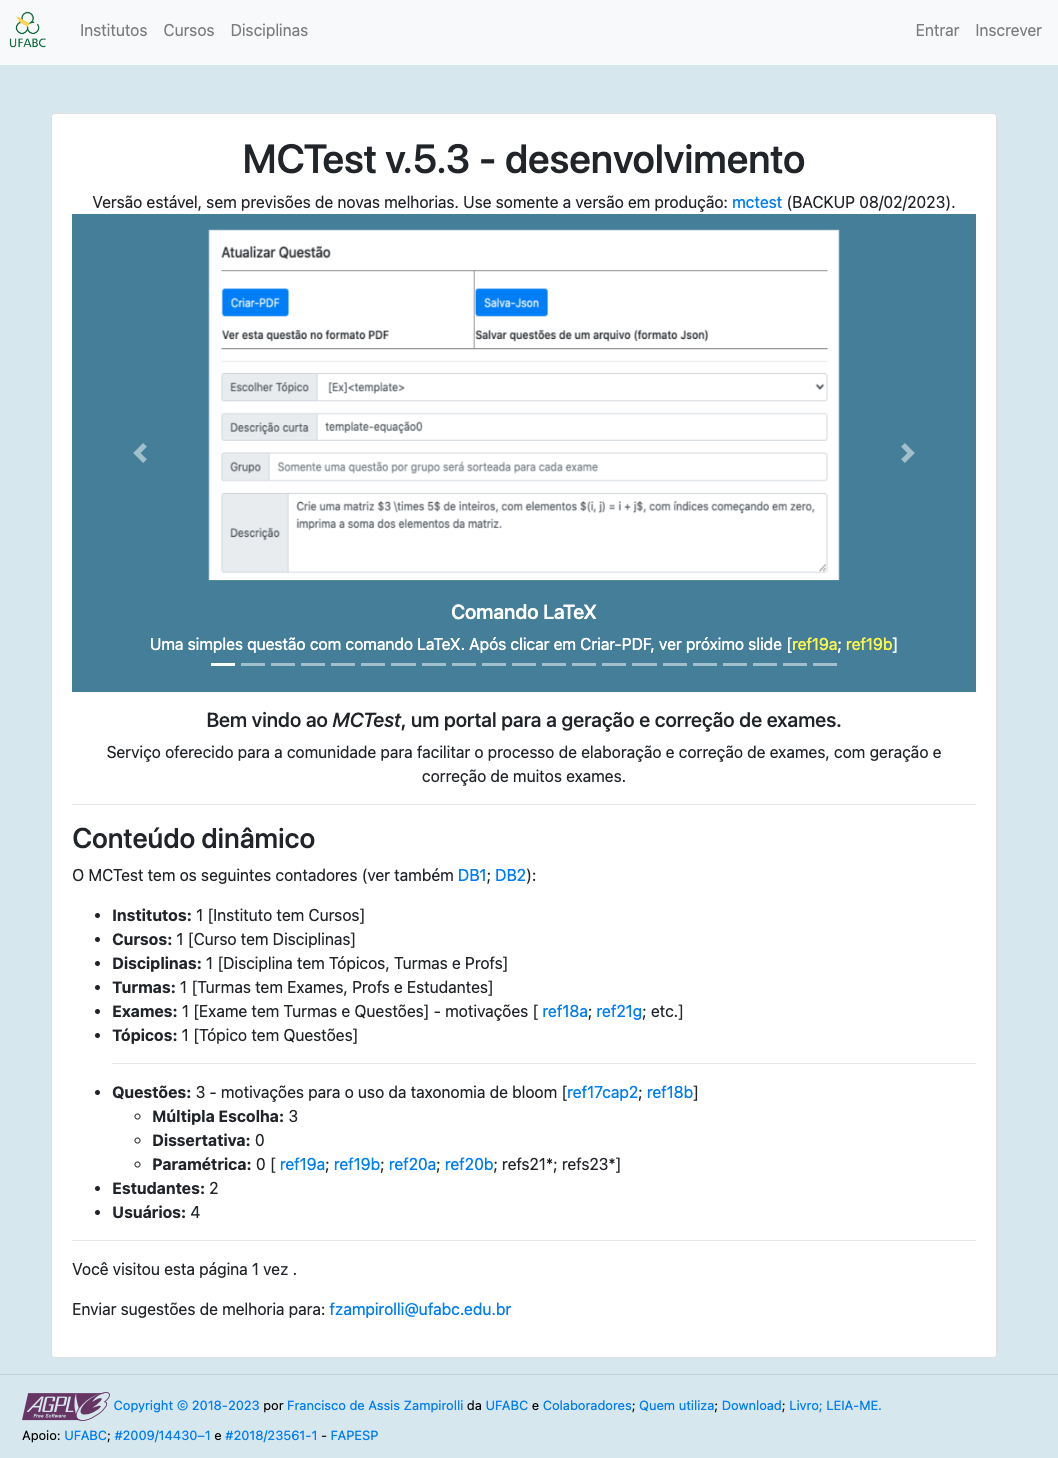
\includegraphics[width=0.9\textwidth]{cap02_figMCTest.png}
  \caption{Tela principal do MCTest.}
  \label{fig:MCTest}
\end{figure}


\begin{mybox}{corObs}{\textbf{Observação:\\\vspace{-3mm}\hrule\vspace{3mm}}}
As figuras apresentadas neste livro correspondem à implantação do MCTest em uma máquina local, utilizando um banco de dados de exemplo disponível no \href{https://github.com/fzampirolli/mctest}{GitHub}, com um número limitado de entidades cadastradas. Para ver um exemplo com um banco de dados mais completo, visite o site \href{http://mctest.ufabc.edu.br}{mctest.ufabc.edu.br}. Para adiantar, o leitor pode instalar uma máquina virtual utilizando o \href{https://www.virtualbox.org/}{VirtualBox} e, em seguida, fazer o \textit{download} de um sistema operacional suportado, conforme explicado no arquivo \href{https://github.com/fzampirolli/mctest/blob/master/_setup-all.sh}{\texttt{\_setup-all.sh}}. Basta seguir as instruções fornecidas nesse arquivo para concluir a instalação, incluindo a instalação das bibliotecas necessárias. É importante notar que o processo de instalação do pacote \LaTeX{} pode levar mais de 10 minutos. Para mais detalhes, ver Seção \ref{sec:instalacao} -- \nameref{sec:instalacao}.
\end{mybox}

Atualmente, além do administrador, o sistema está disponível apenas para usuários do tipo professor, que podem também ser coordenadores de disciplina com permissão para incluir professores e tópicos. O perfil de coordenador é adicionado pelo administrador do sistema ao associá-lo a uma disciplina específica. Cabe ao administrador também a responsabilidade de manter a página do \href{https://www.djangoproject.com/}{Django}.

No MCTest, cada tipo de usuário possui acesso restrito a um conjunto específico de entidades, como ilustrado na Figura \ref{fig:cap2_navegacao}. É importante ressaltar que os itens (c) e (d) são idênticos para professores e coordenadores. Por exemplo, ambos podem visualizar todas as turmas, tópicos e questões das disciplinas em que estão inscritos, mas somente o coordenador pode realizar alterações em tópicos de disciplinas que coordena. Além disso, os menus à esquerda são gerais para todo o conteúdo ao qual o usuário tem acesso, enquanto à direita são apresentados apenas os conteúdos de questões, turmas e exames que o usuário criou. 

\begin{figure}[!ht]
  \centering
  
\includegraphics[width=0.9\textwidth]{cap02_figNavega01.png} 
  \\ (a) Navegação sem estar logado \\ 
  
\includegraphics[width=0.9\textwidth]{cap02_figNavega02.png}
  \\ (b) Navegação para um usuário cadastrado sem perfil \\   
  
\includegraphics[width=0.9\textwidth]{cap02_figNavega03.png}
  \\ (c) Navegação para um usuário com perfil de professor \\ 
  
\includegraphics[width=0.9\textwidth]{cap02_figNavega04.png}
  \\ (d) Navegação para um usuário com perfil de coordenador \\ 
  
\includegraphics[width=0.9\textwidth]{cap02_figNavega05.png}
  \\ (e) Navegação para um usuário com perfil de administrador \\ 
  \caption{Recorte do menu de navegação principal do MCTest.}
  \label{fig:cap2_navegacao}
\end{figure}

O MCTest também permite que um professor coordenador de disciplina adicione vários professores a uma disciplina por um arquivo CSV, sendo automaticamente cadastrado no sistema como perfil de professor (esse processo será exemplificado no próximo capítulo). Com isso, os professores incluídos na disciplina têm acesso somente às funcionalidades do sistema que são relevantes ao seu perfil.

\begin{mybox}{corEdicao2}{\textbf{Destaque:\\\vspace{-3mm}\hrule\vspace{3mm}}}
Para enfatizar um ponto específico no que se refere ao registro de professores, é de extrema relevância ressaltar que, quando um professor efetua seu cadastro de forma independente, ele não é automaticamente incluído no grupo de professores. Nessa situação, torna-se imperativo que um administrador intervenha a fim de efetuar essa inclusão, por meio do acesso à aba ``Admin'', conforme ilustrado na Figura \ref{fig:cap2_navegacao}-(e).
\end{mybox}

Antes de demonstrar como criar entidades no sistema, é importante cadastrar-se na plataforma, clicando na opção ``Inscrever'', conforme indicado na Figura \ref{fig:cap2_navegacao} e exemplificado na Figura \ref{fig:inscrever}. É necessário ressaltar que somente os professores podem se inscrever neste serviço e devem utilizar o e-mail institucional fornecido pela instituição durante o cadastro. Por exemplo, o endereço \texttt{user@ufabc.edu.br} é válido, enquanto \texttt{user@aluno.ufabc.edu.br} é inválido. O e-mail deve conter a URL da instituição (por exemplo, \texttt{@ufabc.edu.br}). Tais restrições são cruciais para garantir a validade e a segurança das informações associadas às instituições cadastradas no sistema. Finalmente, o botão ``De Acordo'', apresentado na Figura \ref{fig:inscrever}, foi detalhado na Seção \ref{sec:deAcordo} -- \nameref{sec:deAcordo}.

\begin{mybox}{pink}{\textbf{Melhorias:\\\vspace{-3mm}\hrule\vspace{1mm}}}
\begin{itemize}
    \item É importante ressaltar que ainda não foi implementada a funcionalidade de segurança para validar o e-mail durante o processo de inscrição. Será necessário implementar essa funcionalidade para garantir a integridade e a segurança dos dados cadastrados no sistema.
    \item Outra melhoria importante para a segurança do sistema é a utilização de um certificado digital, que permitirá a utilização do protocolo HTTPS em vez de HTTP nos servidores utilizados para a implantação do MCTest. O HTTPS criptografa a comunicação entre o navegador do usuário e o servidor, garantindo a confidencialidade e a integridade dos dados transmitidos. 
\end{itemize}
\end{mybox}

\begin{figure}[!ht]
  \centering
  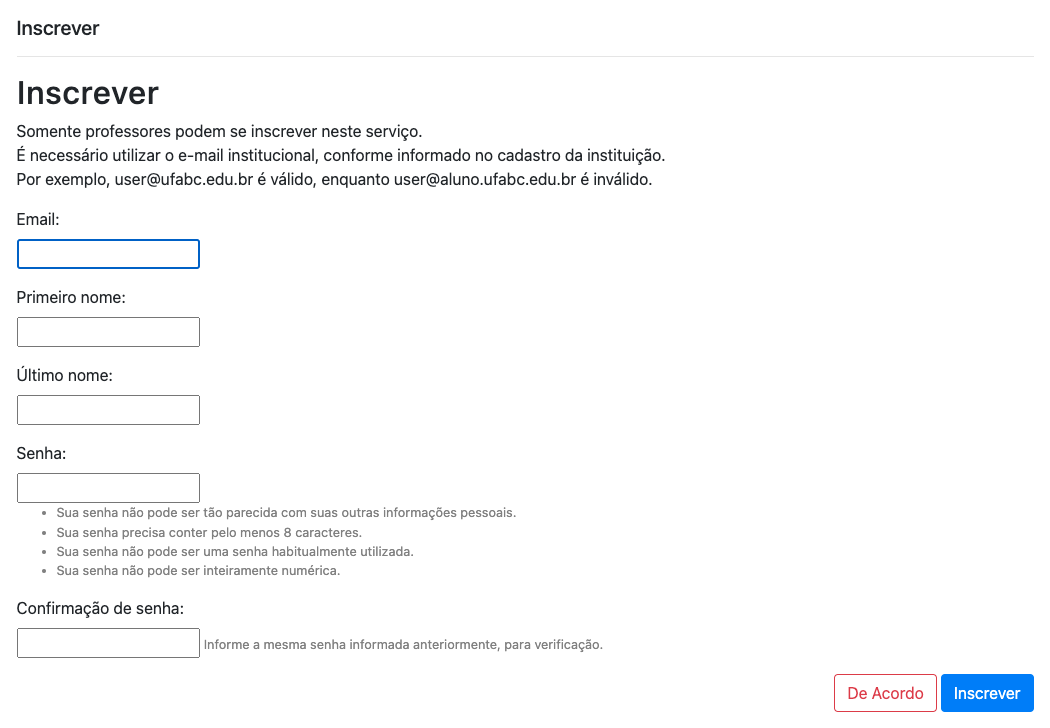
\includegraphics[width=0.9\textwidth]{cap02_figInscrever.png} 
  \caption{Tela para a inscrição do usuário.}
  \label{fig:inscrever}
\end{figure}

\section{Criar entidades}

O MCTest é um sistema que gerencia diversas entidades em um banco de dados MySQL, como detalhado neste e no próximo capítulo. Essas entidades são criadas e relacionadas para modelar o domínio educacional com foco na avaliação dos estudantes. Além disso, o sistema oferece funcionalidades para o cadastro, alteração, remoção e consulta dessas entidades e seus relacionamentos.

Nesta seção, você encontrará a descrição das principais entidades de negócio de um sistema educacional que tem como foco as avaliações. É importante ressaltar que, embora as entidades, questão e exame sejam de extrema importância no contexto do MCTest, elas serão abordadas em capítulos específicos para uma exposição mais detalhada e aprofundada.

\subsection{Instituto}\label{sec:instituto}

A entidade instituto representa a instituição cadastrada no sistema e contém atributos como nome, código, logo, site, entre outros.
%
A criação de uma entidade instituto é restrita ao usuário com perfil de administrador. 

Na Figura \ref{fig:instituto}, ao clicar em ``Criar um novo Instituto'', uma tela será aberta para cadastrar informações sobre o instituto, conforme ilustrado na Figura \ref{fig:cap02_figInstitutoCria}. Ao clicar em um instituto existente na coluna ``Código'' ou ``Nome'' da Figura \ref{fig:instituto}, o usuário será direcionado para uma tela para visualizar as informações do instituto, conforme ilustrado na Figura \ref{fig:cap02_figInstitutoDetalha}. É importante observar que nesta tela também é apresentada a lista de cursos, que será detalhada na próxima seção. 

Ao clicar no botão ``Atualizar'' em um instituto existente na coluna ``Ações'' da Figura \ref{fig:instituto}, o usuário será direcionado para uma nova tela para atualizá-lo, semelhante à Figura \ref{fig:cap02_figInstitutoCria}. Se o usuário clicar em ``Apagar'', o instituto será removido do banco de dados, após confirmação na janela de diálogo apresentada na Figura \ref{fig:cap02_figInstitutoRemover}.


\begin{figure}[!ht]
  \centering
  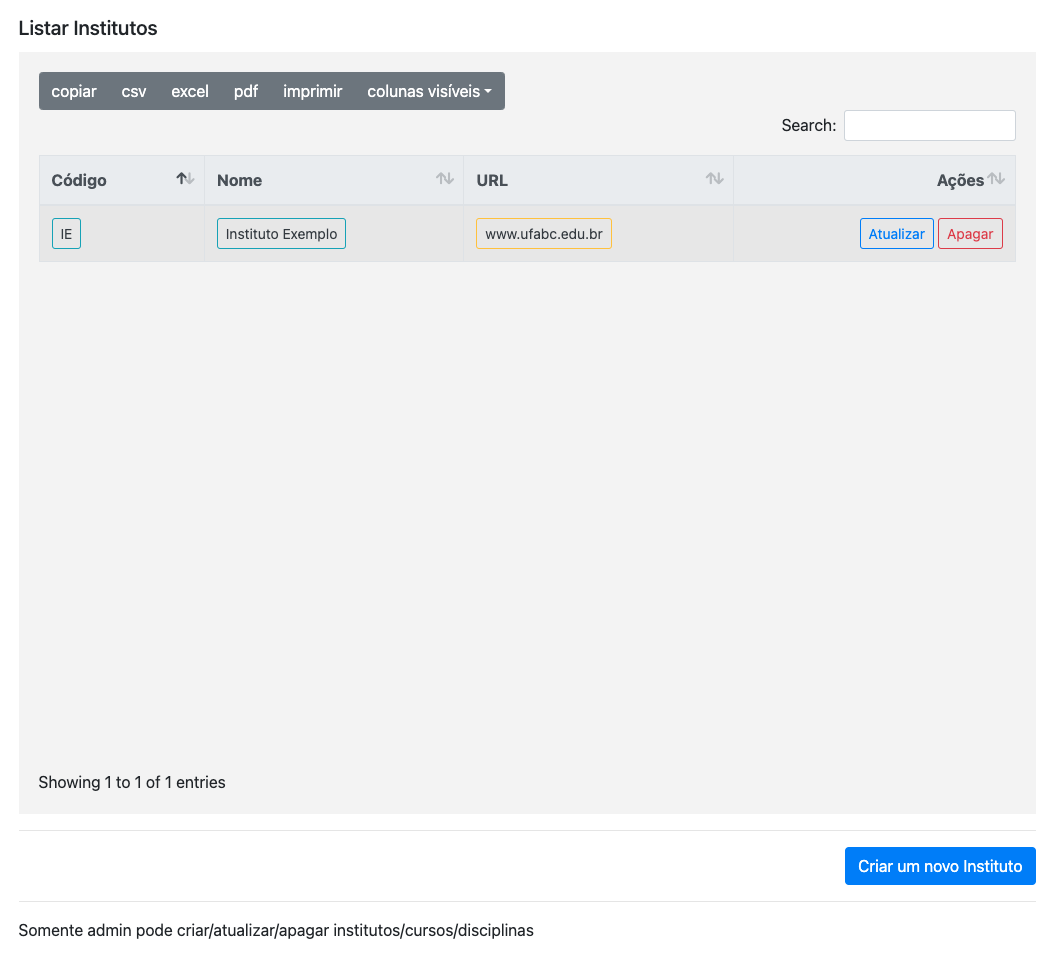
\includegraphics[width=0.9\textwidth]{cap02_figInstituto.png}
  \caption{Tela para administrador atualizar, apagar ou criar um instituto.}
  \label{fig:instituto}
\end{figure}

A Figura \ref{fig:cap02_figInstitutoCria} apresenta o recorte da tela para ``Criar de um novo Instituto'', que é similar à de ``Atualizar um Instituto''. Os três últimos campos exibidos na tela são utilizados para contabilizar o número de exames e questões gerados e corrigidos pelo sistema desde a criação do instituto. Esses contadores são úteis para monitorar a atividade do sistema em relação a cada instituto.
%
É importante ressaltar que apenas o administrador pode zerar esses contadores a qualquer momento, o que pode ser necessário em algumas circunstâncias, como quando é necessário reiniciar as contagens ou avaliar a atividade recente do sistema.

\begin{figure}[!ht]
  \centering
  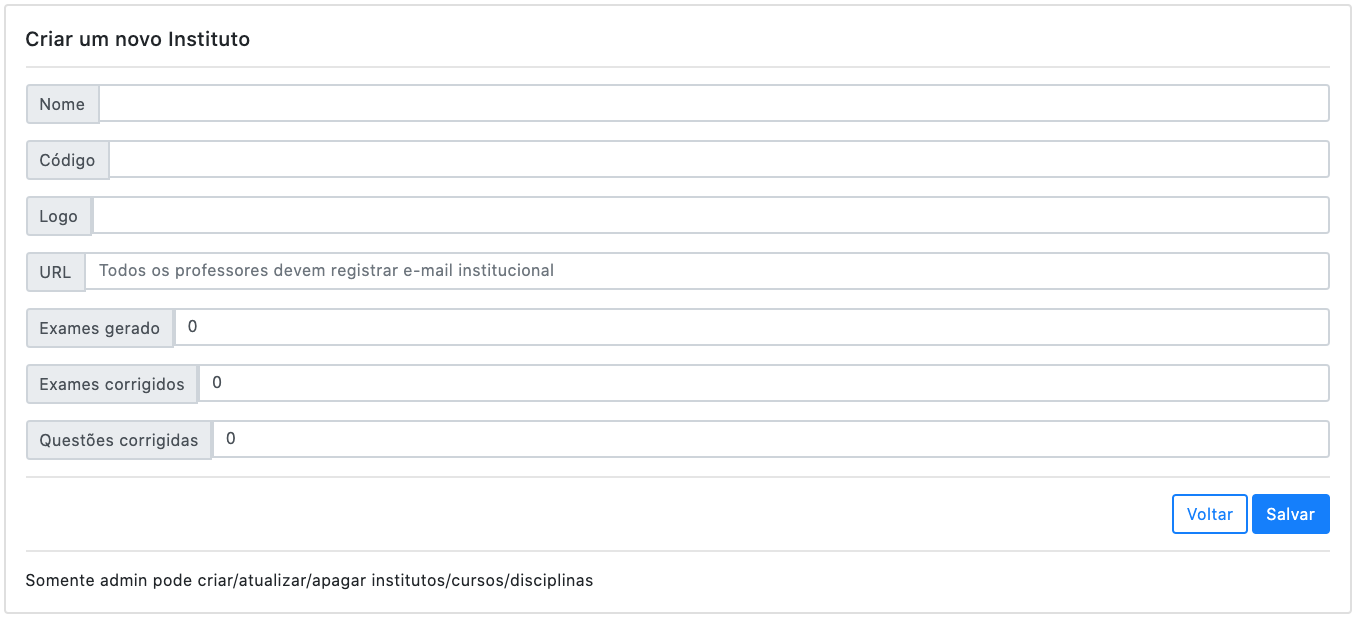
\includegraphics[width=0.9\textwidth]{figs-br/cap02_figInstitutoCria.png}
  \caption{Tela para o administrador criar um instituto.}
  \label{fig:cap02_figInstitutoCria}
\end{figure}


\begin{mybox}{corObs}{\textbf{Observação:\\\vspace{-3mm}\hrule\vspace{3mm}}}
As telas e as ações de criar, ler, atualizar e remover (CRUD -- \textit{Create, Read, Update, Delete}) para fazer a manutenção do instituto são semelhantes, em geral, às demais entidades do MCTest. Portanto, a partir deste ponto, serão apresentadas apenas as telas com informações diferentes, para o usuário poder se concentrar nas especificidades da manutenção das entidades do sistema.
Além disso, os nomes dessas entidades nessas telas devem seguir o formato \LaTeX.
\end{mybox}


\begin{figure}[!ht]
  \centering
  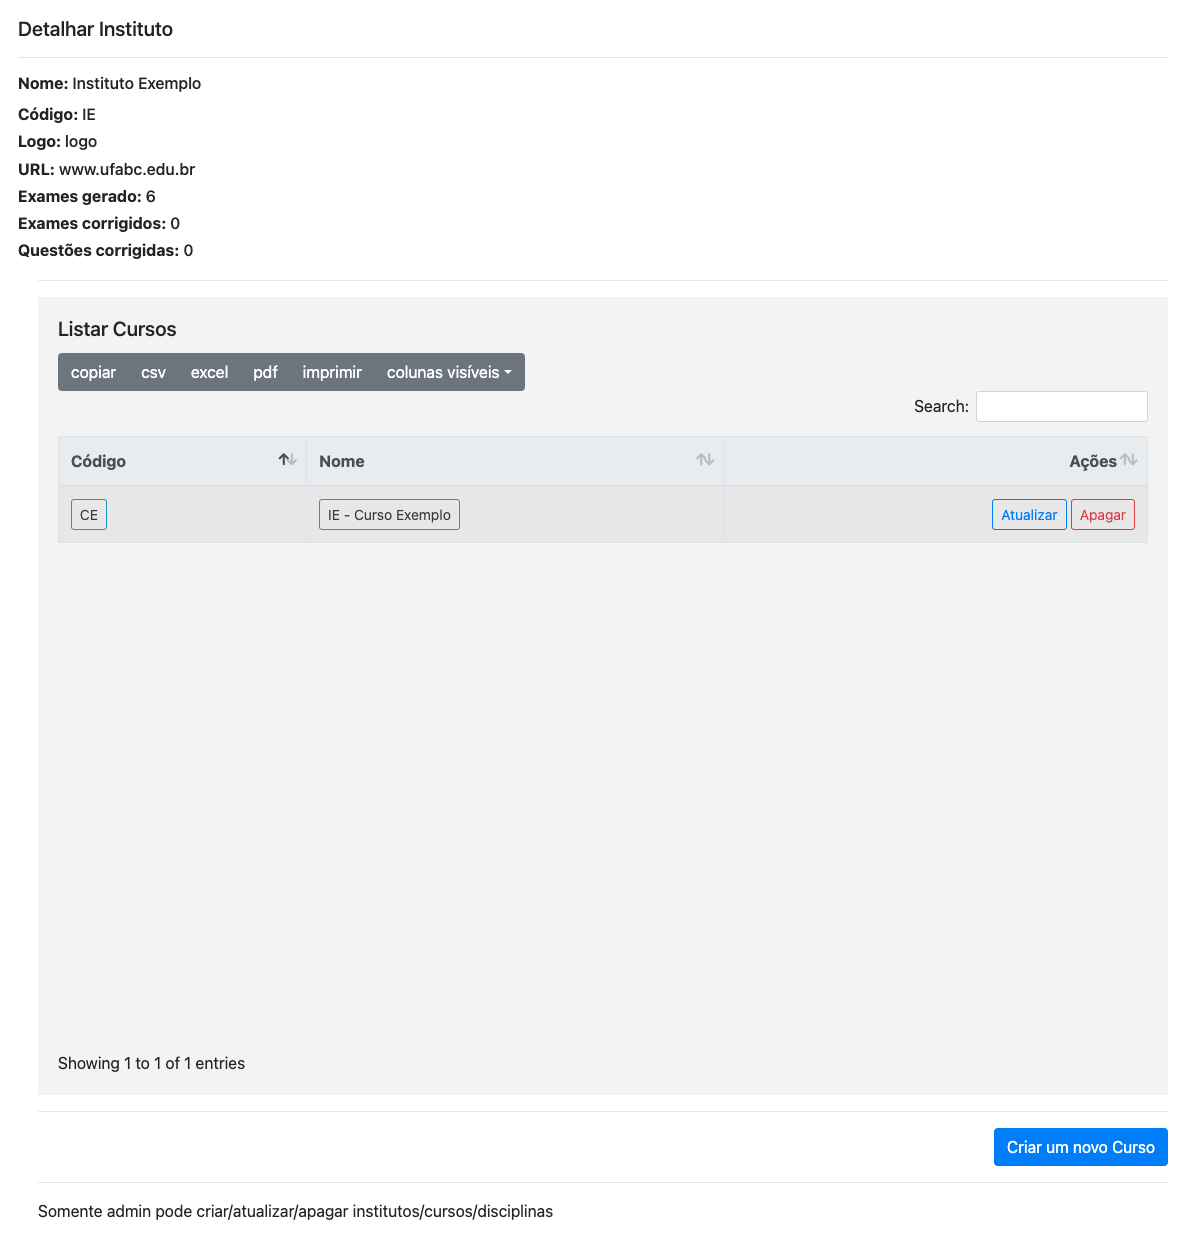
\includegraphics[width=0.9\textwidth]{cap02_figInstitutoDetalha.png}
  \caption{Tela apresentando os detalhes de um instituto.}
  \label{fig:cap02_figInstitutoDetalha}
\end{figure}

\begin{figure}[!ht]
  \centering
  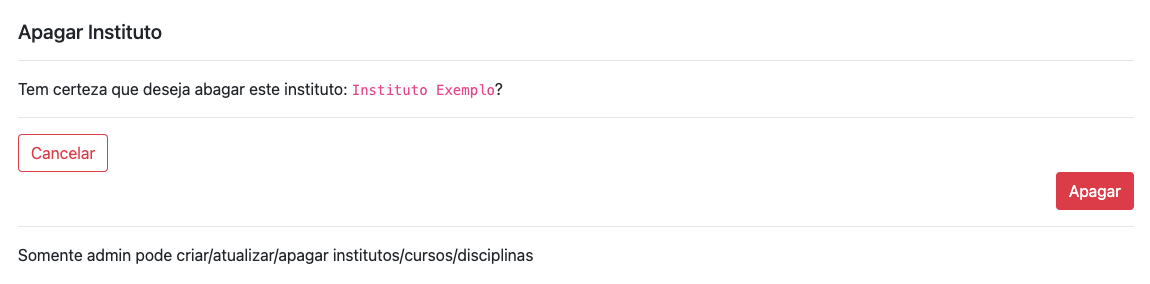
\includegraphics[width=0.9\textwidth]{cap02_figInstitutoRemover.png}
  \caption{Tela para confirmar a exclusão do instituto.}
  \label{fig:cap02_figInstitutoRemover}
\end{figure}

% \newpage

% \ \\ \ 

% \newpage

% \ \\ \ 

% \newpage

\subsection{Curso}\label{sec:curso}

A criação da entidade curso é restrita ao usuário com perfil de administrador, como ilustrado na Figura \ref{fig:curso}, que também pode atualizar ou apagar um curso existente, conforme apresentado na coluna ``Ações'' (outros tipos de usuários não têm acesso a esses botões). É importante destacar que um curso pode pertencer a um ou vários institutos, permitindo assim a organização dos cursos de acordo com sua área de atuação ou afinidade temática.

Na UFABC, por exemplo, um instituto como o Centro de Matemática, Computação e Cognição (CMCC) pode conter vários cursos. Além disso, um curso pode pertencer a mais de um instituto, e existem também cursos intercentros, como o Bacharelado em Ciência e Tecnologia (BCT), que pode pertencer ao instituto PROGRAD (Pró-Reitoria de Graduação) e também aos três centros existentes na UFABC.

Outros exemplos de cursos na UFABC incluem a Escola Preparatória, que pode ser um curso do instituto PROEC (Pró-Reitoria de Extensão e Cultura), e o curso de idiomas, que pertence ao instituto NETEL (Núcleo Educacional de Tecnologias e Línguas), entre outros. 

\begin{figure}[!ht]
  \centering
  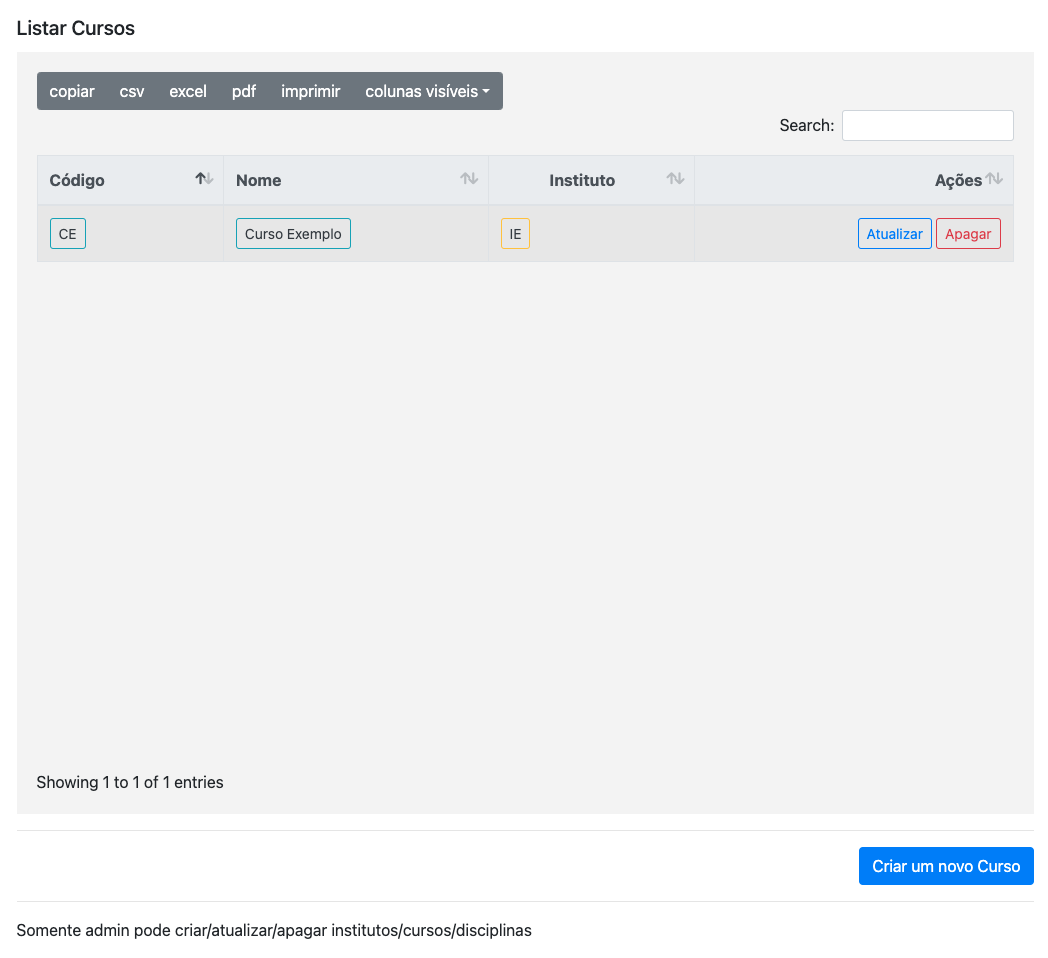
\includegraphics[width=0.9\textwidth]{cap02_figCurso.png}
  \caption{Tela que apresenta a lista de cursos, na qual o administrador pode atualizar, apagar ou criar um novo curso.}
  \label{fig:curso}
\end{figure}

Essa flexibilidade na associação dos cursos aos institutos permite uma maior customização do sistema de avaliação educacional do MCTest, conforme as necessidades específicas de cada instituição ou curso. Dessa forma, é possível adaptar o sistema para atender às demandas e particularidades de diferentes áreas de conhecimento e instituições de ensino.

Ao clicar no botão ``Criar um novo Curso'' na Figura \ref{fig:curso}, o administrador será direcionado para a tela de criação de um novo curso, apresentada na Figura \ref{fig:cursoCria}. Nesta tela, o administrador deve preencher as informações necessárias sobre o curso, como o nome e código. Além disso, é necessário selecionar o instituto ao qual o curso pertence, como exemplificado no caso do ``Instituto Exemplo''. É importante destacar que é possível associar mais de um instituto a um curso específico, como será exemplificado no próximo capítulo. Após preencher todas as informações, o administrador deve clicar no botão ``Salvar'' para salvar o curso no banco de dados do sistema.

\begin{figure}[!ht]
  \centering
  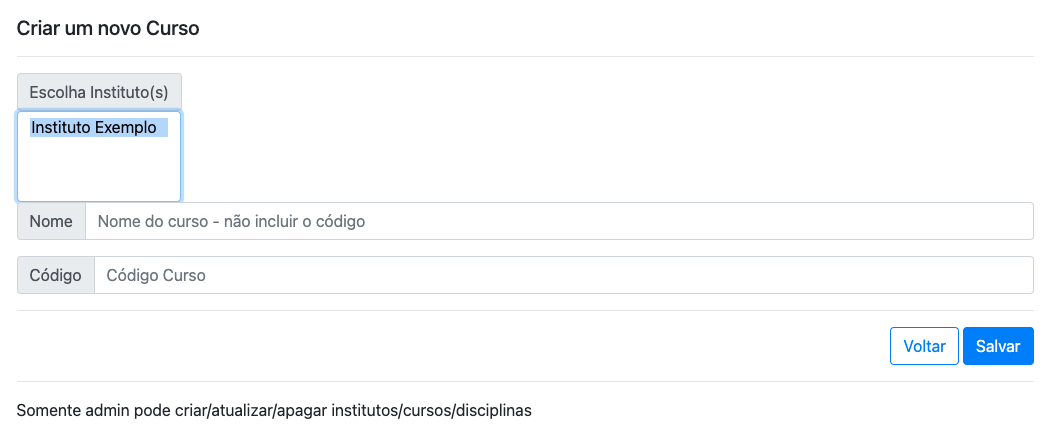
\includegraphics[width=0.9\textwidth]{cap02_figCursoCria.png}
  \caption{Tela para administrador criar um curso novo.}
  \label{fig:cursoCria}
\end{figure}

\begin{mybox}{pink}{\textbf{Melhorias:\\\vspace{-3mm}\hrule\vspace{3mm}}}
   É importante destacar que o banco de dados do sistema já suporta o relacionamento entre um conjunto de professores/coordenadores e uma instituição/curso. Portanto, é necessário implementar as funcionalidades que permitam vincular esses profissionais às entidades correspondentes. Isso permitirá que a gestão dos professores/coordenadores seja feita de forma mais organizada e eficiente, facilitando a alocação desses profissionais em diferentes cursos ou instituições. 
\end{mybox}


Ao clicar em um curso nas colunas ``Código'' ou ``Nome'' na Figura \ref{fig:curso}, o usuário será direcionado para uma tela detalhando as informações do curso selecionado, conforme ilustrado na Figura \ref{fig:cap02_figCursoDetalha}. É importante observar que nesta tela também são inseridas informações sobre as disciplinas do curso selecionado, em forma de uma lista. A manutenção das disciplinas será abordada na próxima seção.

\begin{figure}[!ht]
  \centering
  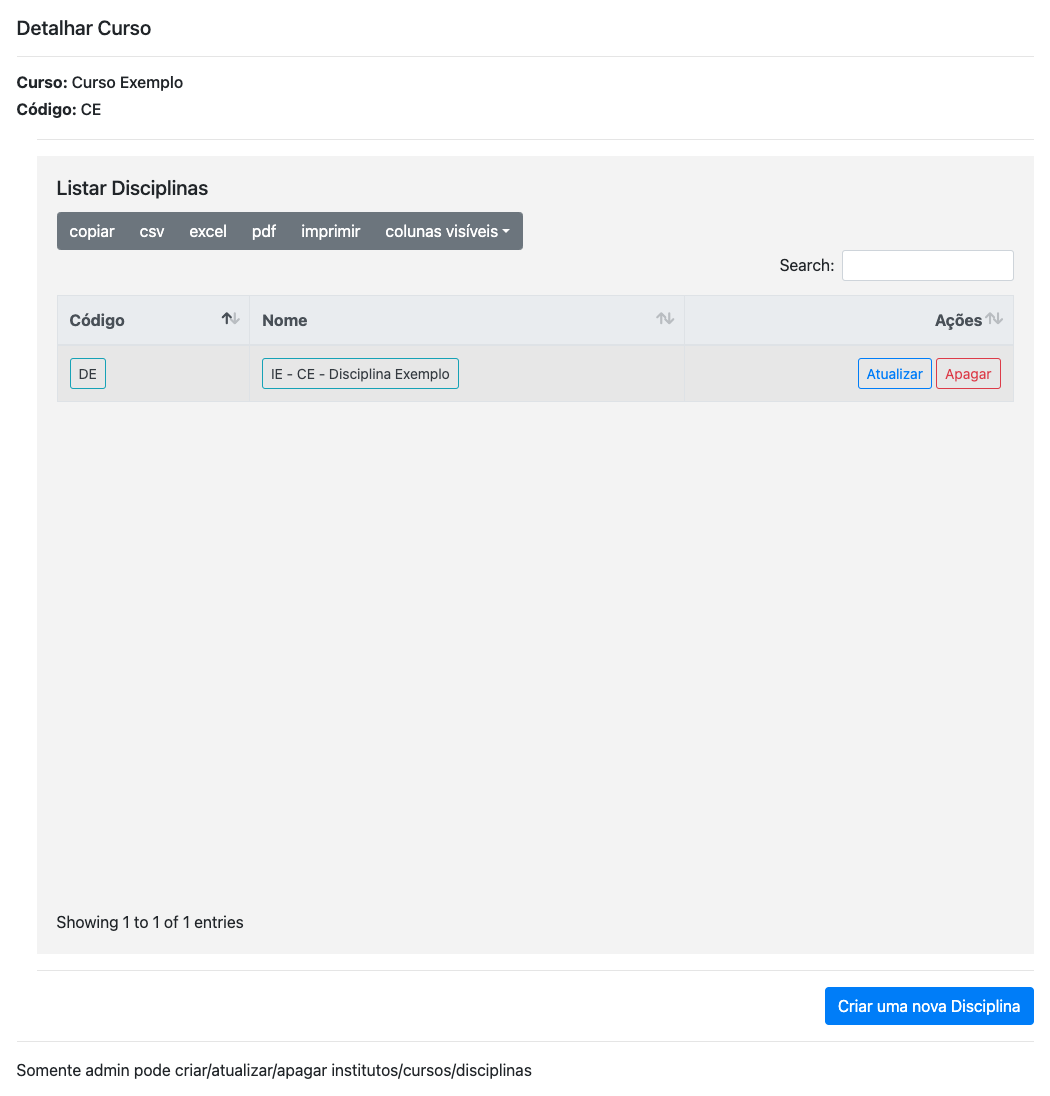
\includegraphics[width=0.9\textwidth]{cap02_figCursoDetalha.png}
  \caption{Tela apresentando os detalhes de um curso.}
  \label{fig:cap02_figCursoDetalha}
\end{figure}

% \newpage

% \ \\ \ 

% \newpage

% \ \\ \ 

\subsection{Disciplina}\label{sec:disciplina}

A entidade disciplina é responsável por representar as disciplinas cadastradas no sistema, sendo sua criação restrita ao usuário com perfil de administrador, que também pode atualizar ou apagar uma disciplina existente, como ilustrado na Figura \ref{fig:cap02_figDisciplina}, conforme apresentado na coluna ``Ações'' (outros tipos de usuários não têm acesso a esses botões de ação). No entanto, o usuário com perfil de coordenador possui permissão apenas para atualizar a disciplina que coordena, como será detalhado na próxima seção.

A entidade disciplina é essencial para a organização das turmas e tópicos, o que permite criar exames específicos para atender a várias turmas simultaneamente, facilitando a gestão e a aplicação de avaliações na plataforma.

\begin{figure}[!ht]
  \centering
  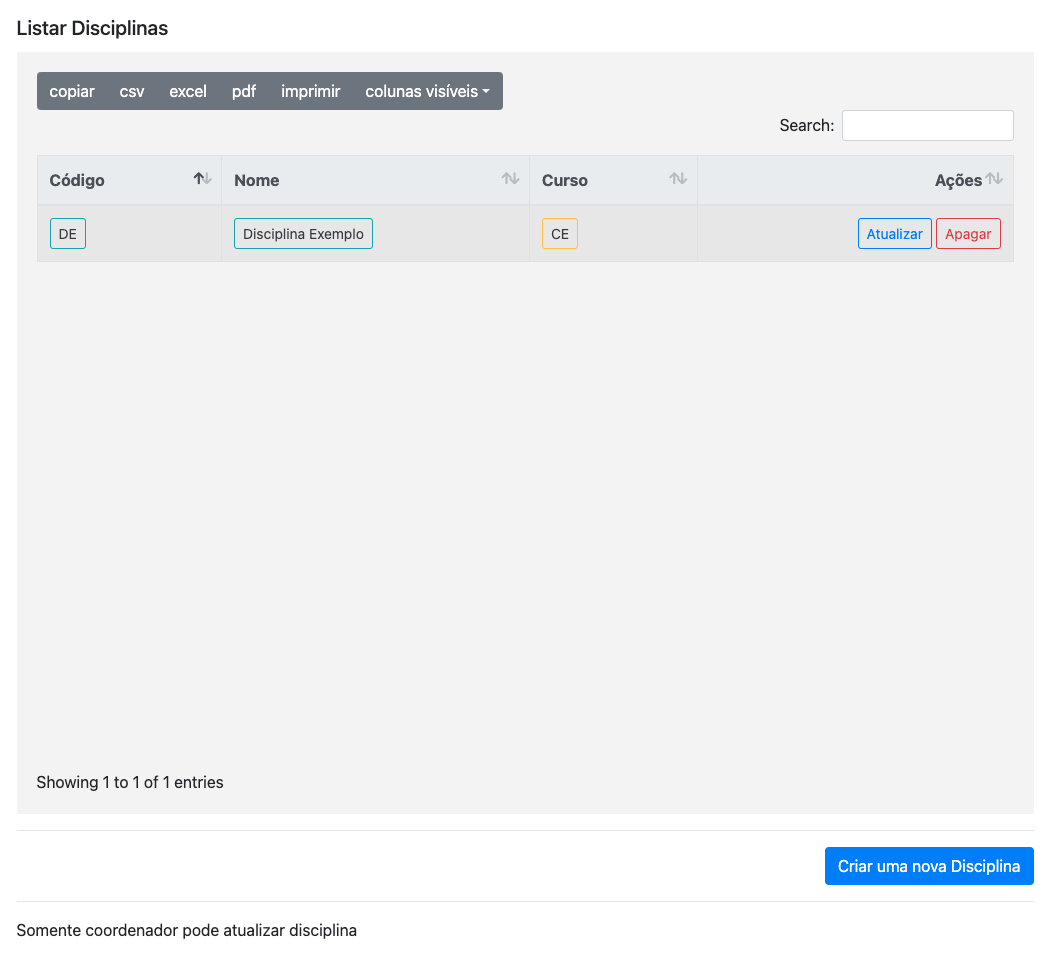
\includegraphics[width=0.9\textwidth]{cap02_figDisciplina.png}
  \caption{Tela que apresenta a lista de disciplinas, na qual o administrador pode atualizar, apagar ou criar uma nova disciplina.}
  \label{fig:cap02_figDisciplina}
\end{figure}

A Figura \ref{fig:cap02_figDisciplinaCria} mostra a tela para criar uma disciplina. Esta tela é semelhante à primeira parte da tela de atualização de uma disciplina. No caso de uma disciplina com muitas turmas, foram implementadas funcionalidades na segunda parte da tela de atualização de disciplina para o coordenador poder cadastrar todos os professores e estudantes de várias turmas de uma só vez, através da importação de arquivos no formato CSV, conforme ilustrado na Figura \ref{fig:cap02_figDisciplinaAtualiza22}. Essa funcionalidade será detalhada no próximo capítulo, na Seção \ref{sec:variasTurmasCSV}  -- \nameref{sec:variasTurmasCSV}.

A flexibilidade na associação de cursos permite uma personalização maior do sistema de avaliação educacional do MCTest, conforme as necessidades específicas de cada disciplina. Além disso, é possível associar professores e coordenadores à disciplina, permitindo uma organização mais eficiente e atribuição de responsabilidades na gestão da disciplina. Para selecionar mais de um professor, basta manter a tecla \textbf{Ctrl} pressionada.

É fundamental destacar que a criação e associação de disciplinas aos cursos devem ser realizadas com cautela e atenção pelo coordenador, visando garantir a precisão e efetividade da avaliação educacional. A associação correta de disciplinas aos respectivos cursos, institutos e professores é crucial para a realização de exames precisos e eficazes.

\begin{figure}[!ht]
  \centering
  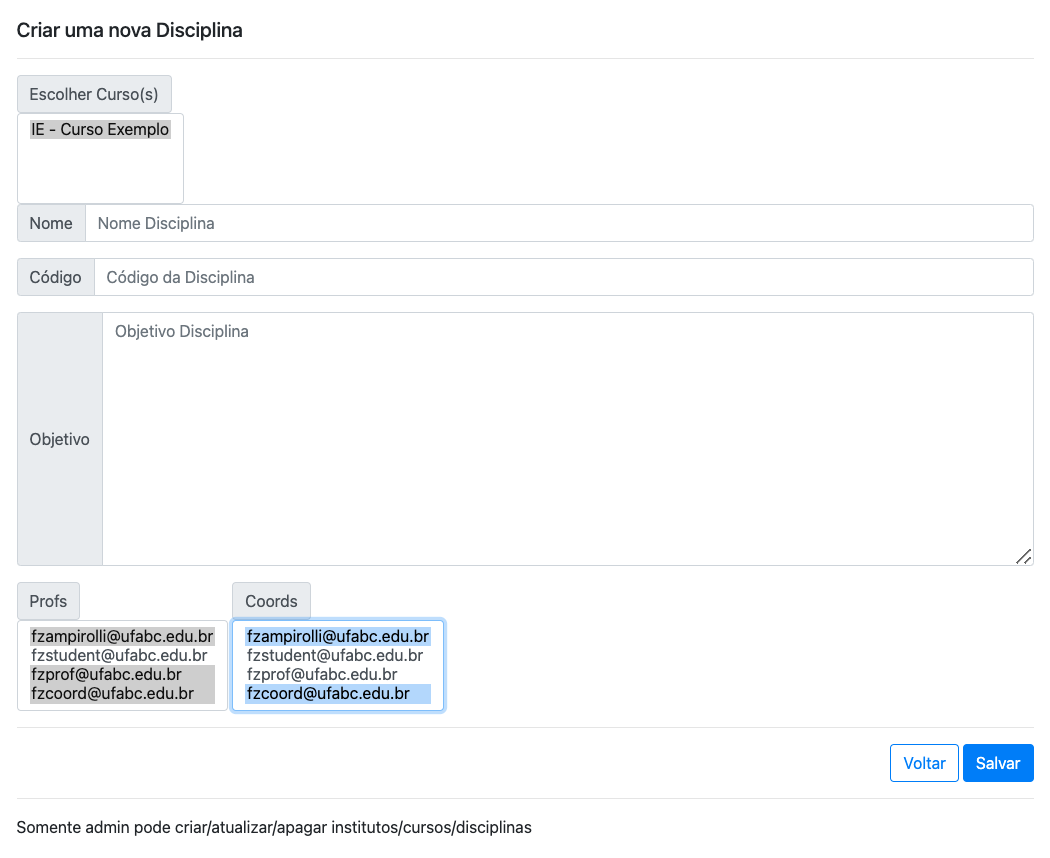
\includegraphics[width=0.9\textwidth]{cap02_figDisciplinaCria.png}
  \caption{Tela para o administrador criar uma disciplina. Tela semelhante à primeira parte da tela de atualizar uma disciplina.}
  \label{fig:cap02_figDisciplinaCria}
\end{figure}

\begin{figure}[!ht]
  \centering
  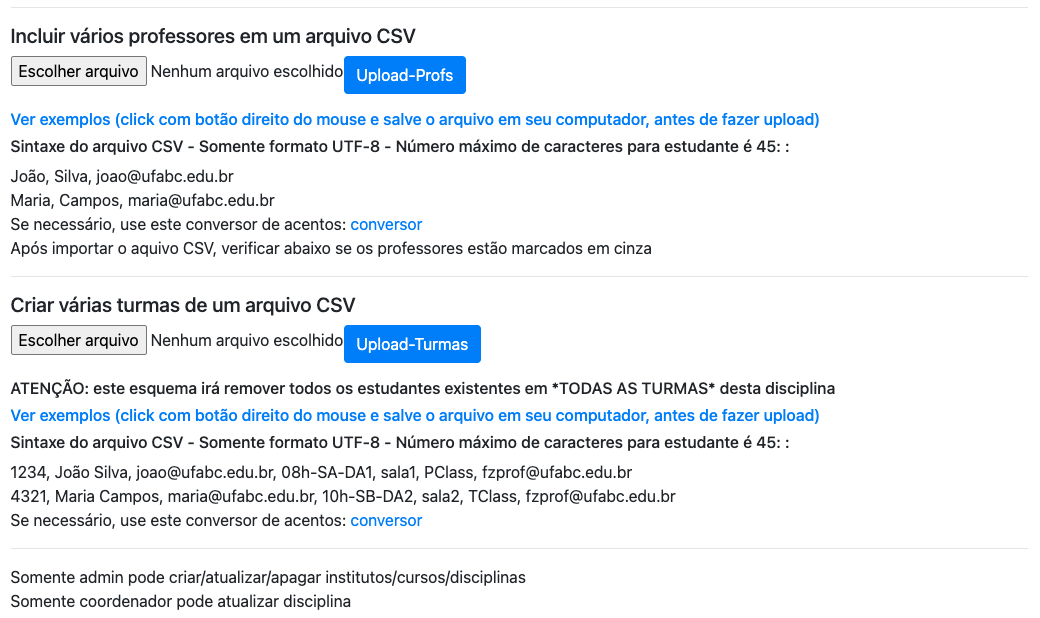
\includegraphics[width=0.9\textwidth]{cap02_figDisciplinaAtualiza2.png}
  \caption{Segunda parte da tela para o administrador atualizar uma disciplina.}
  \label{fig:cap02_figDisciplinaAtualiza22}
\end{figure}

Ao clicar em uma disciplina nas colunas ``Código'' ou ``Nome'' da Figura \ref{fig:cap02_figDisciplina}, será aberta uma tela detalhando as informações da disciplina, conforme ilustrado nas Figuras \ref{fig:cap02_figDisciplinaDetalha} e \ref{fig:cap02_figDisciplinaDetalha2}.

\begin{figure}[!ht]
  \centering
  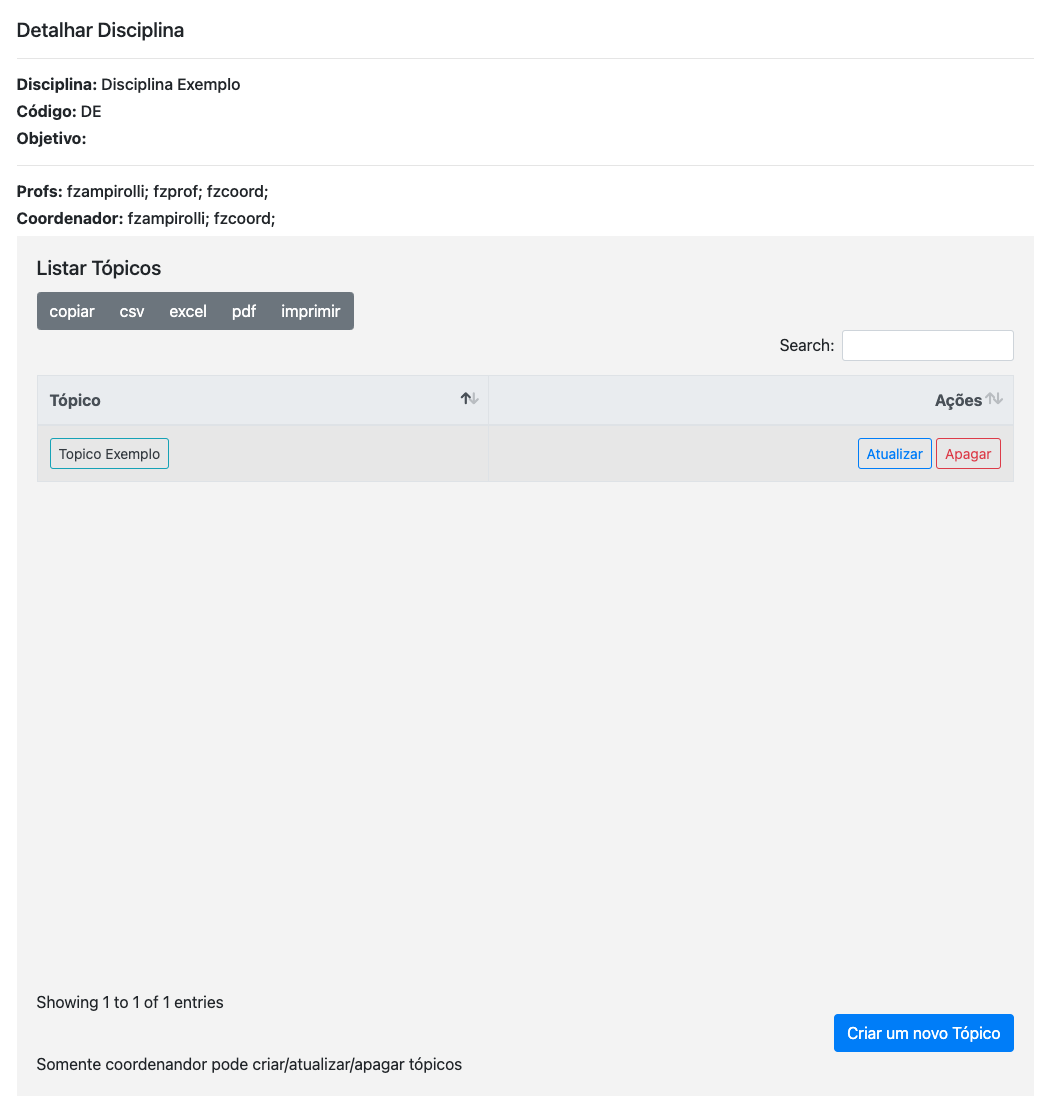
\includegraphics[width=0.9\textwidth]{cap02_figDisciplinaDetalha.png}
  \caption{(Parte 1) Tela apresentando os detalhes de uma disciplina.}
  \label{fig:cap02_figDisciplinaDetalha}
\end{figure}

\begin{figure}[!ht]
  \centering
  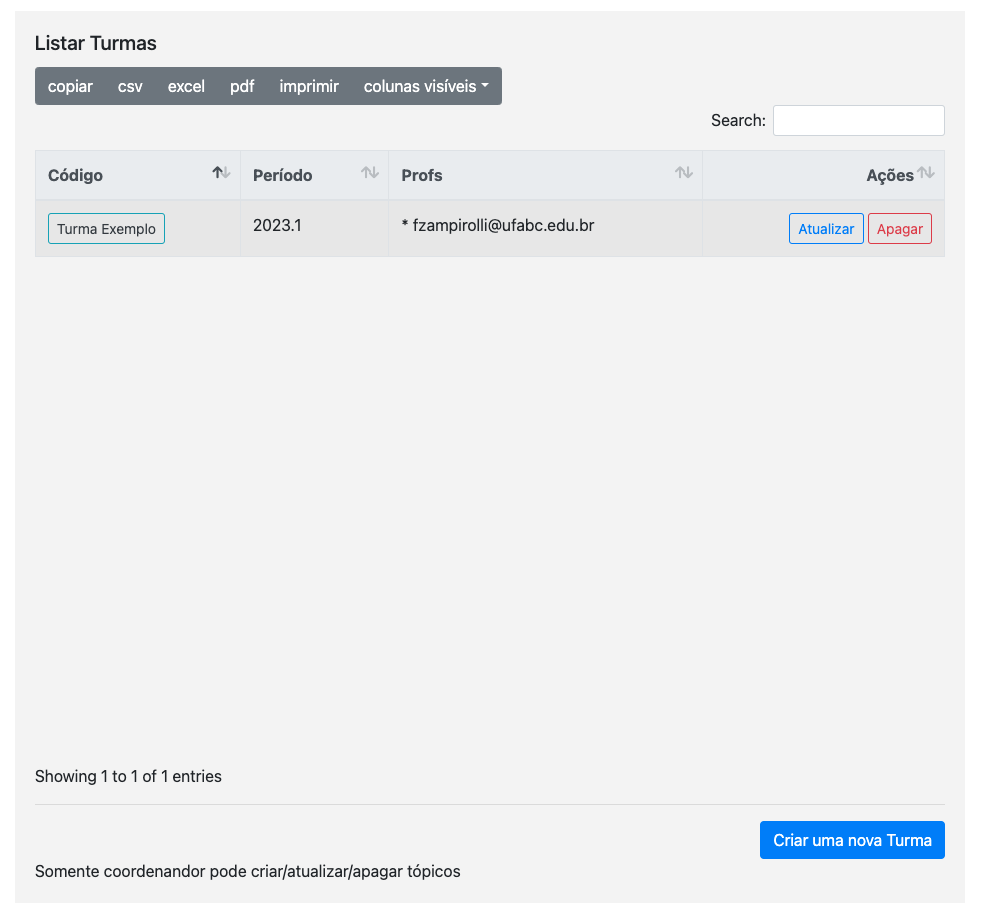
\includegraphics[width=0.9\textwidth]{cap02_figDisciplinaDetalha2.png}
  \caption{(Parte 2) Continuação da tela apresentando os detalhes de uma disciplina.}
  \label{fig:cap02_figDisciplinaDetalha2}
\end{figure}

% \newpage

% \ \\ \ 

% \newpage

% \ \\ \ 

% \newpage

% \ \\ \ 

% \newpage

% \ \\ \ 

% \newpage

% \ \\ \ 

\subsection{Turma}\label{sec:turma}

A entidade turma é responsável por representar as turmas cadastradas para cada disciplina no MCTest. A criação, atualização ou exclusão de turmas pode ser realizada pelo administrador, pelo coordenador ou pelo professor da disciplina, conforme apresentado na Figura \ref{fig:cap02_figTurma}. Nesta figura, o professor tem a opção de criar uma nova turma ao clicar em ``Criar uma nova Turma'', abrindo a tela apresentada na Figura \ref{fig:cap02_figTurmaCriar}. Para isso, é necessário escolher uma disciplina, definir o código da sala da disciplina e especificar se a turma é de teoria ou prática.

\begin{figure}[!ht]
  \centering
  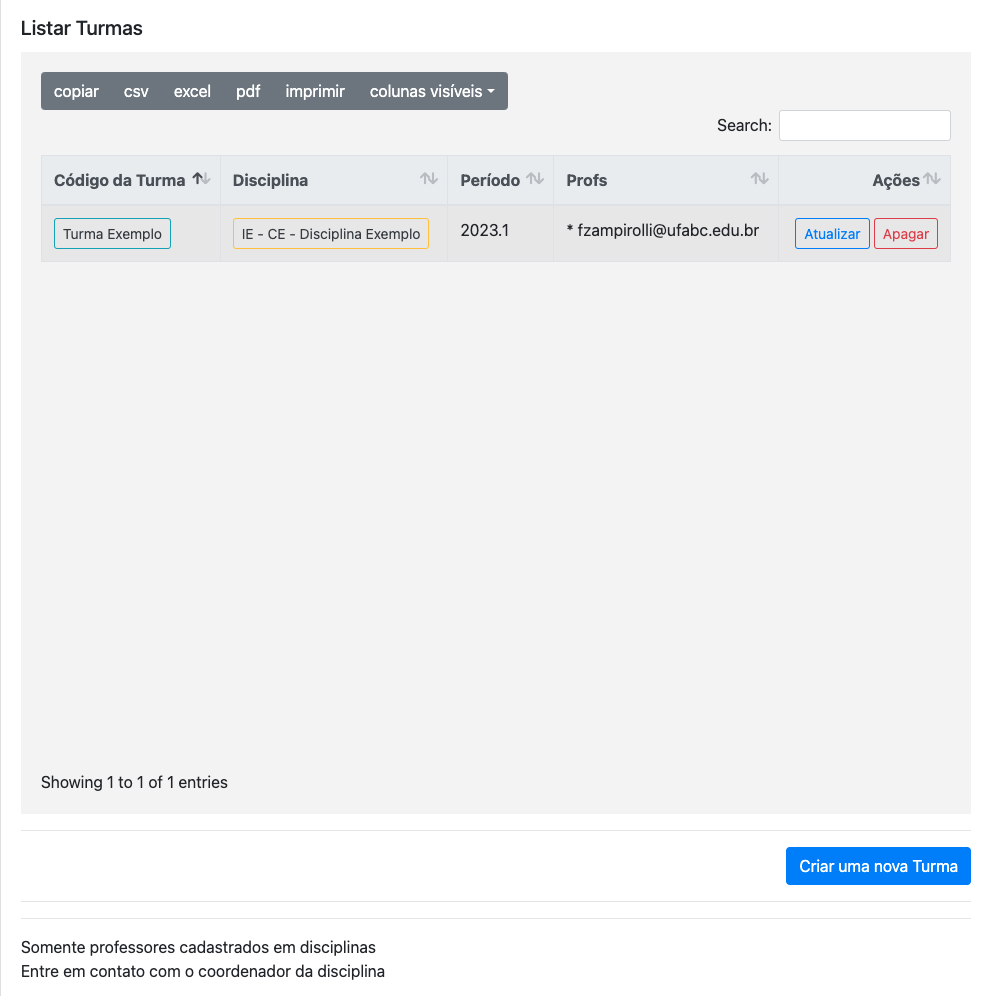
\includegraphics[width=0.9\textwidth]{cap02_figTurma.png}
  \caption{Tela que apresenta a lista de turmas, na qual um professor de uma disciplina pode criar uma nova turma, além de atualizar ou apagar turmas existentes.}
  \label{fig:cap02_figTurma}
\end{figure}



\begin{figure}[!ht]
  \centering
  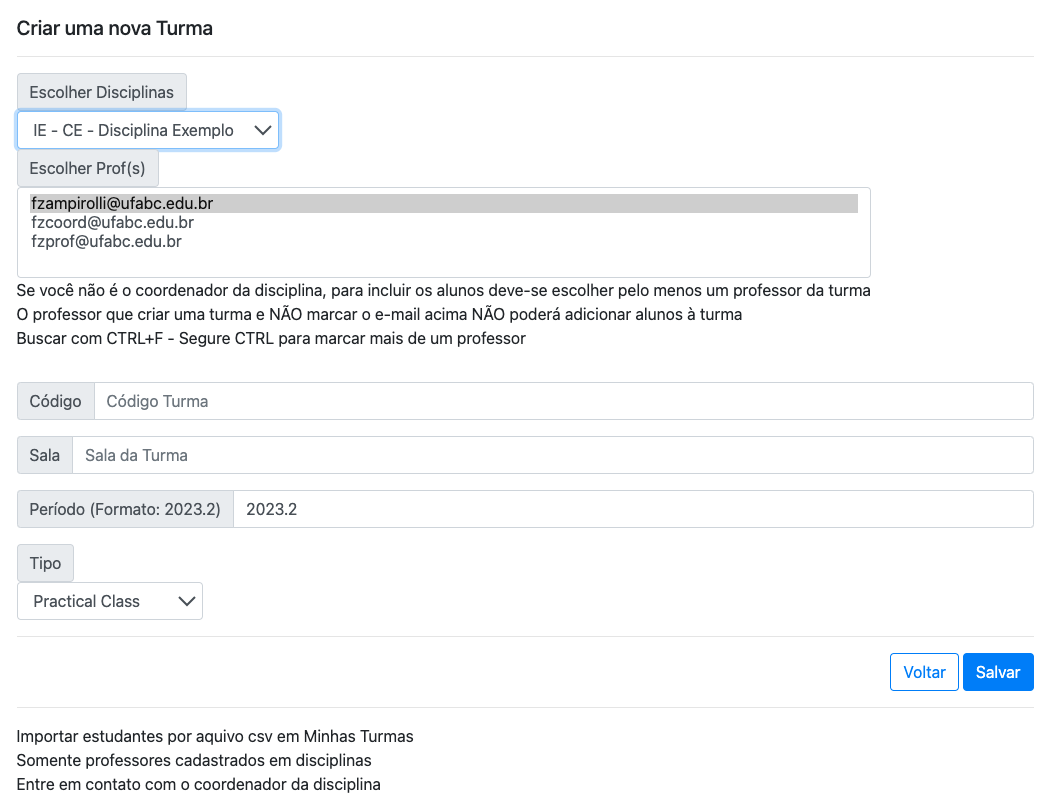
\includegraphics[width=0.9\textwidth]{cap02_figTurmaCriar.png}
  \caption{Tela utilizada pelo professor para criar uma nova turma após clicar no botão ``Criar uma nova Turma'', na tela da Figura \ref{fig:cap02_figTurma}. É importante destacar que o nome da turma não pode conter acentos ou caracteres especiais, pois esse nome fará parte do cabeçalho do exame.}
  \label{fig:cap02_figTurmaCriar}
\end{figure}

Após a criação da turma pelo professor, a tela apresentada na Figura \ref{fig:cap02_figTurma} deve ser atualizada e é possível clicar em ``Atualizar'' na coluna ``Ações'' para inserir estudantes na turma. Essa ação levará à tela de atualização da turma, conforme ilustrado na Figura \ref{fig:cap02_figTurmaAtualiza}. Nessa tela, é possível fazer a importação de um arquivo no formato CSV contendo a lista de estudantes que serão adicionados à turma.

\begin{figure}[!ht]
  \centering
  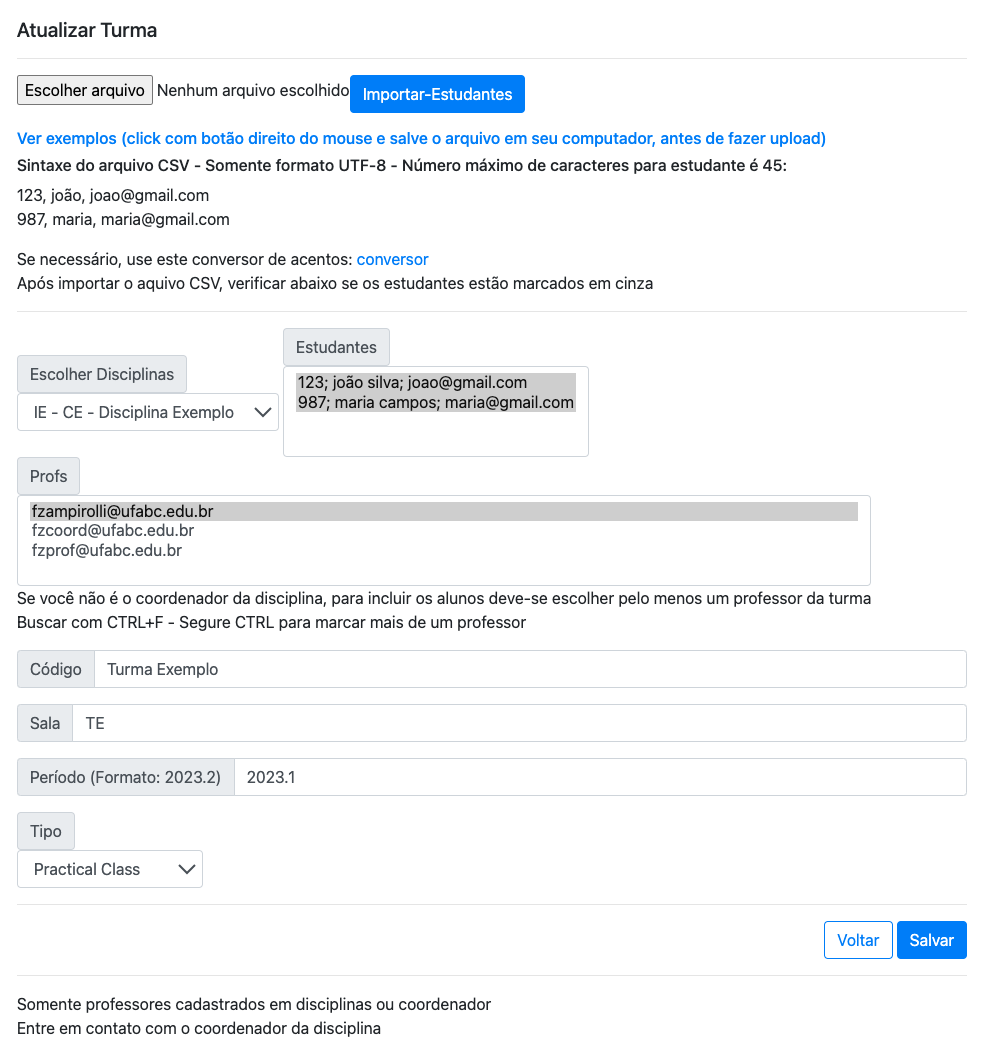
\includegraphics[width=0.9\textwidth]{cap02_figTurmaAtualiza.png}
  \caption{Tela para um professor de uma disciplina poder atualizar uma turma, inserindo estudantes com a importação de um arquivo no formato CSV.}
  \label{fig:cap02_figTurmaAtualiza}
\end{figure}

Na Figura \ref{fig:cap02_figTurma}, o professor pode clicar no código da turma (primeira coluna), o que exibe a tela apresentada na Figura \ref{fig:cap02_figTurmaAtualiza2}. Nessa tela, é possível atualizar ou apagar estudantes. A Figura \ref{fig:cap02_figTurmaAtualiza3} apresenta a tela utilizada para atualizar os dados de um estudante.

Na Figura \ref{fig:cap02_figTurmaAtualiza}, é possível observar uma lista de todas as disciplinas do professor, se houver alguma, em ``Escolher Disciplinas''. Ao clicar no código de uma turma específica (primeira coluna), o professor pode acessar a tela apresentada na Figura \ref{fig:cap02_figTurmaAtualiza2}.


\begin{figure}[!ht]
  \centering
  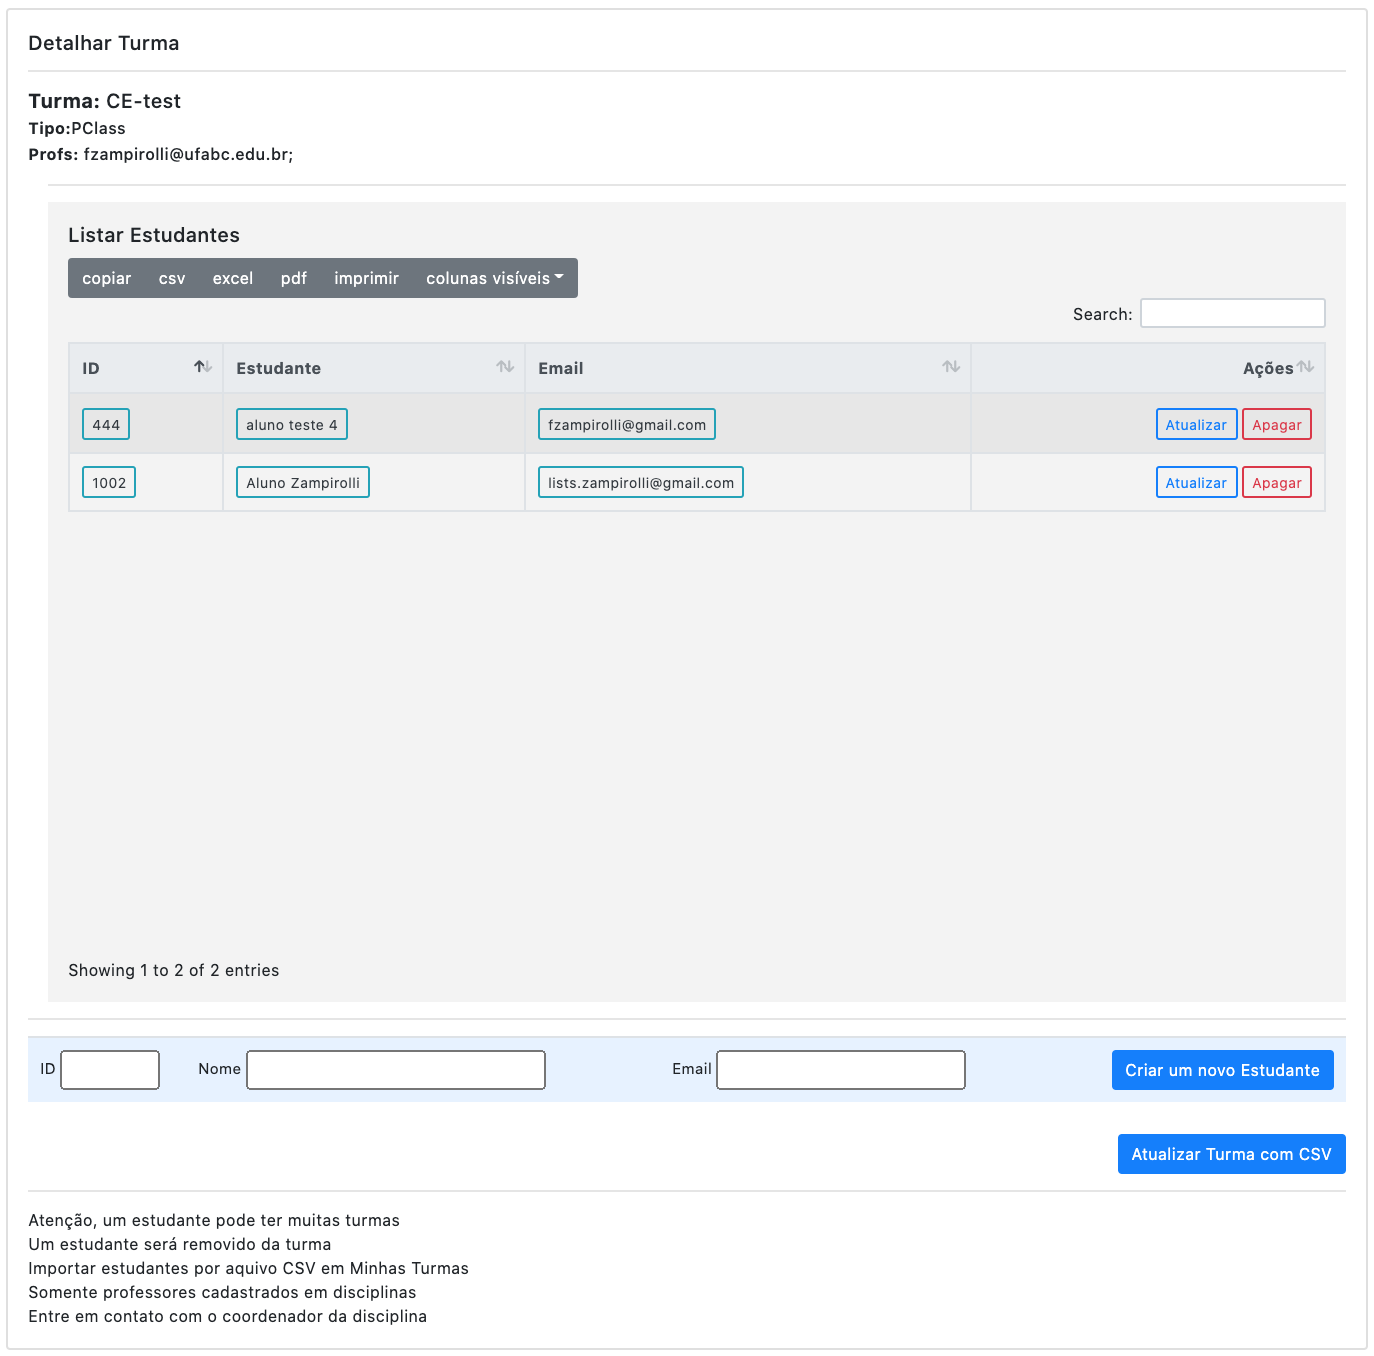
\includegraphics[width=0.9\textwidth]{cap02_figTurmaAtualiza2.png}
  \caption{Tela para um professor de uma disciplina poder atualizar uma turma, atualizando ou apagando estudantes da turma. Além disso, é possível incluir um novo estudante na turma.}
  \label{fig:cap02_figTurmaAtualiza2}
\end{figure}

Além disso, ao clicar no nome de um estudante específico, o professor acessa a tela mostrada na Figura \ref{fig:cap02_figTurmaAtualiza3}, na qual é possível atualizar dados do estudante, como nome, e-mail e matrícula. Essa funcionalidade permite aos professores manter a lista de estudantes atualizada e corrigir eventuais erros ou inconsistências nas informações.

\begin{figure}[!ht]
  \centering
  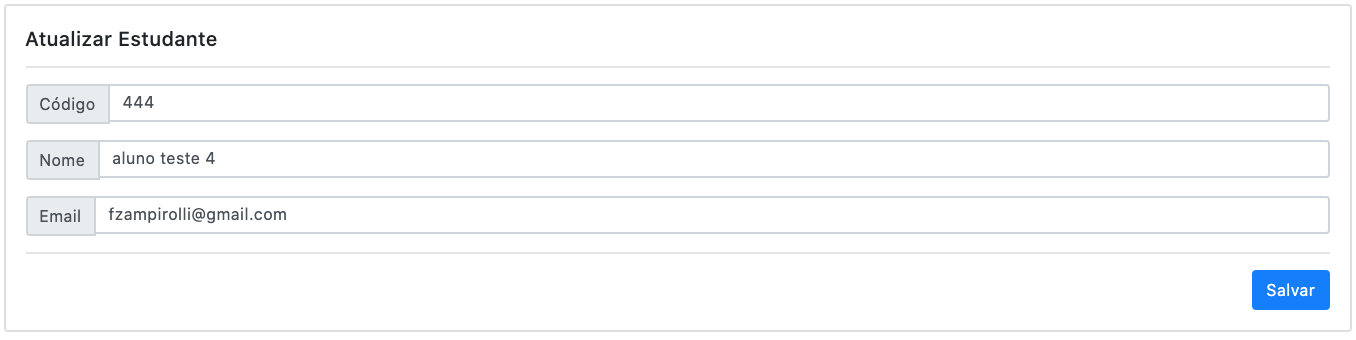
\includegraphics[width=0.9\textwidth]{cap02_figTurmaAtualiza3.png}
  \caption{Tela para um professor de uma disciplina poder atualizar os dados de um estudante da turma.}
  \label{fig:cap02_figTurmaAtualiza3}
\end{figure}

% \newpage

% \ \\ \ 

% \newpage

% \ \\ \ 

% \newpage

\subsection{Tópico}\label{sec:topicos}

Os tópicos são utilizados para organizar questões dentro de uma disciplina, sendo que cada disciplina possui um conjunto específico de tópicos associados. A criação, atualização ou exclusão de tópicos em disciplinas é permitida apenas para usuários com perfil de coordenador ou administrador, conforme ilustrado na lista de tópicos apresentada na Figura \ref{fig:cap02_figTopico}. Vale destacar que a lista exibida corresponde aos tópicos das disciplinas nas quais o usuário possui participação.

\begin{figure}[!ht]
  \centering
  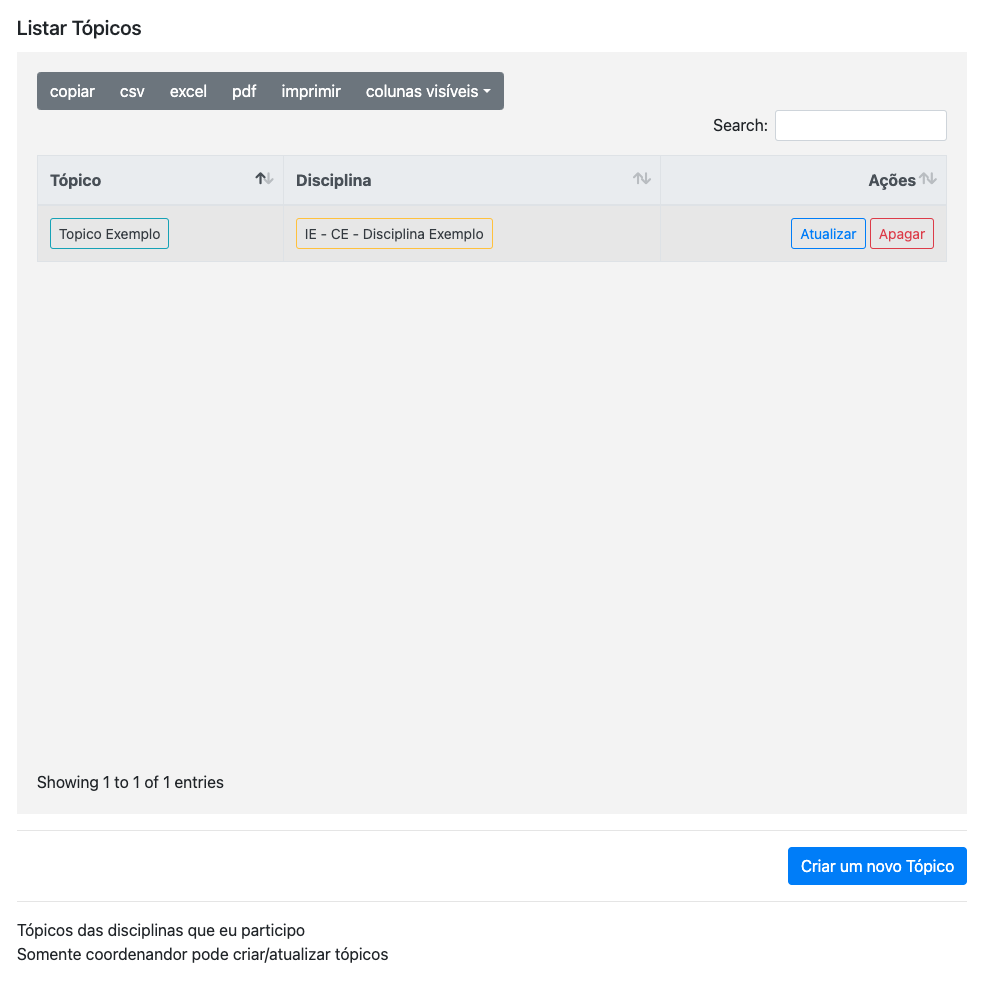
\includegraphics[width=0.9\textwidth]{cap02_figTopico.png}
  \caption{Tela com a lista de tópicos para o coordenador (ou administrador) criar, atualizar ou apagar um tópico de disciplina(s).}
  \label{fig:cap02_figTopico}
\end{figure}

A Figura \ref{fig:cap02_figTopicoAtualiza} apresenta a tela para atualização de um tópico, que é semelhante à tela de cadastro de um novo tópico. Uma das principais funcionalidades disponíveis nessa tela é a possibilidade de associar mais de uma disciplina ao tópico em questão, mantendo a tecla \texttt{Ctrl} pressionada. Essa flexibilidade permite que um mesmo tópico possa ser utilizado em diferentes disciplinas, conforme as necessidades e particularidades de cada uma delas.

\begin{figure}[!ht]
  \centering
  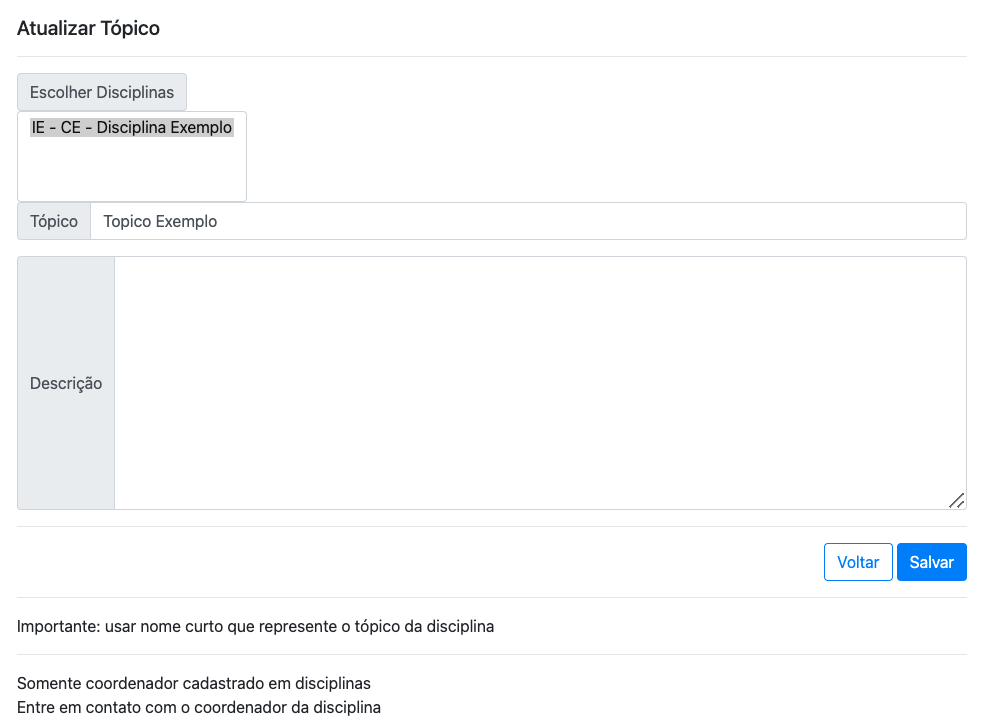
\includegraphics[width=0.9\textwidth]{cap02_figTopicoAtualiza.png}
  \caption{Tela para o coordenador (ou administrador) atualizar um tópico de uma disciplina.}
  \label{fig:cap02_figTopicoAtualiza}
\end{figure}

Ao clicar em um tópico na primeira coluna da Figura \ref{fig:cap02_figTopico}, será aberta uma tela detalhando as questões relacionadas ao tópico, conforme ilustrado na Figura \ref{fig:cap02_figTopicoDetalha} (as outras colunas serão detalhadas nos próximos capítulos). É importante destacar o botão ``Criar-PDF'', que permite a criação de um arquivo PDF contendo todas as questões do tópico selecionado, conforme ilustrado na Figura \ref{fig:cap02_figTopicoDetalha2}. Detalhes sobre este arquivo serão abordados em capítulos futuros.

\begin{figure}[!ht]
  \centering
  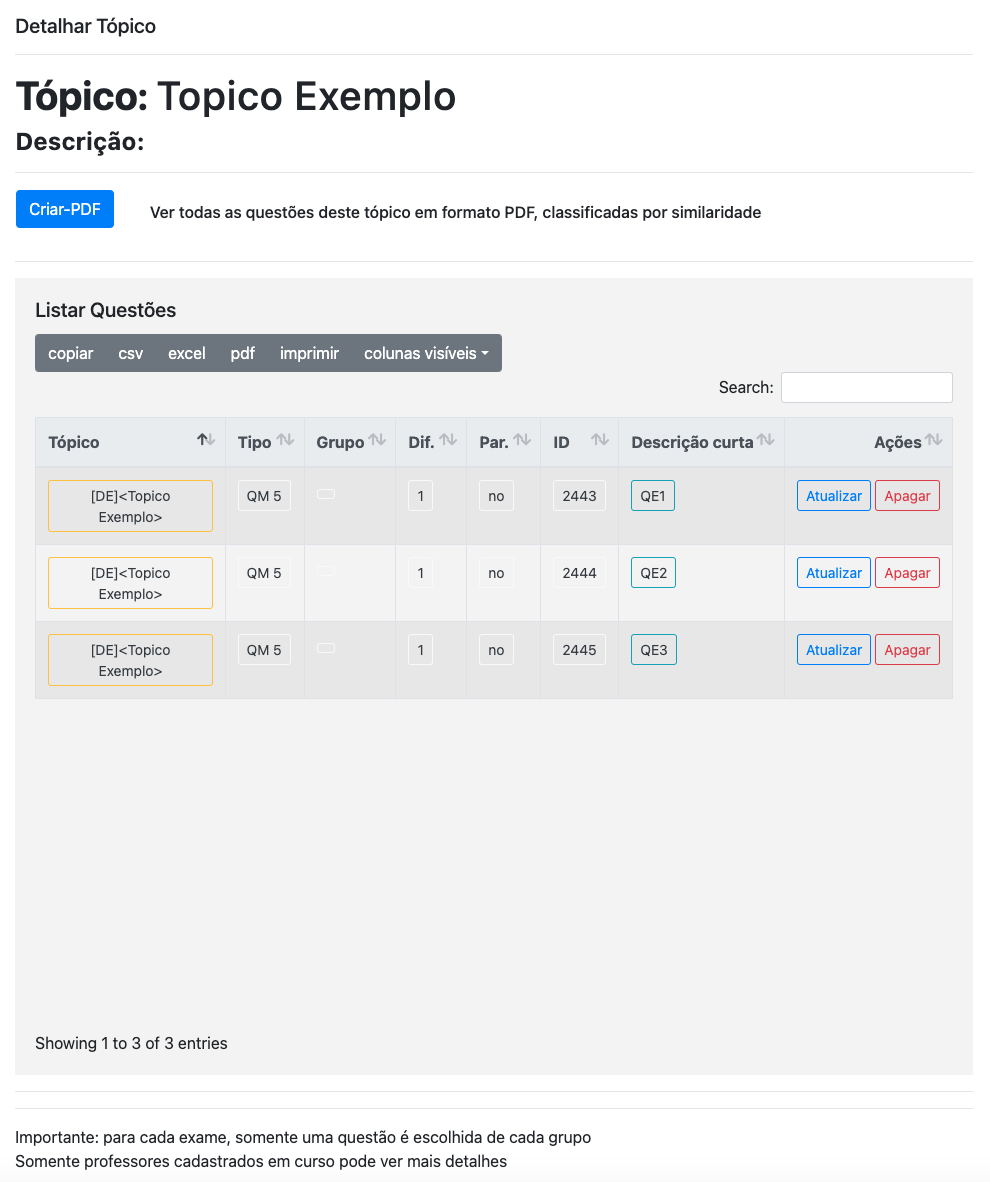
\includegraphics[width=0.9\textwidth]{cap02_figTopicoDetalha.png}
  \caption{Tela apresentando os detalhes de um tópico.}
  \label{fig:cap02_figTopicoDetalha}
\end{figure}

\begin{figure}[!ht]
  \centering
  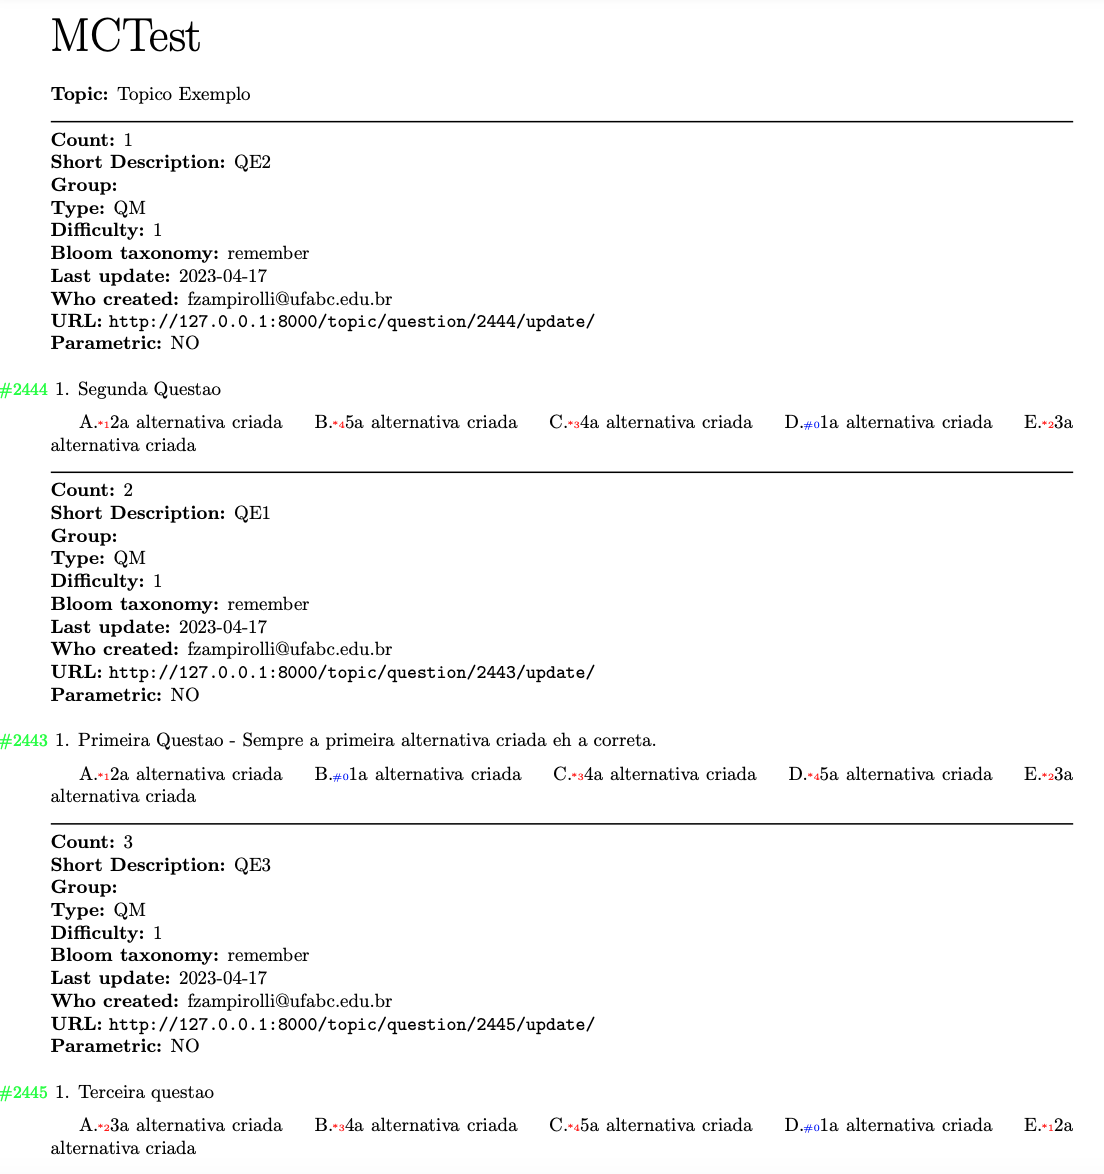
\includegraphics[width=0.9\textwidth]{cap02_figTopicoDetalha2.png}
  \caption{Tela apresentando as três primeiras questões de um tópico.}
  \label{fig:cap02_figTopicoDetalha2}
\end{figure}

% \newpage

% \ \\ \ 

% \newpage

% \ \\ \ 

% \newpage

% \ \\ \ 

% \newpage

\section{Considerações finais}

Neste capítulo, foi apresentada uma visão geral do MCTest, enfatizando sua estrutura e funcionalidades essenciais. Foi discutida a navegação geral do sistema, destacando como os usuários podem acessar as diferentes entidades disponíveis, como institutos, cursos, disciplinas, turmas e tópicos.

Os diferentes tipos de usuários com acesso ao MCTest foram apresentados, incluindo administrador, coordenador e professor, juntamente com suas respectivas permissões e responsabilidades específicas.

O administrador foi identificado como o usuário com maior privilégio, possuindo acesso irrestrito a todas as funcionalidades e dados do sistema. Sua responsabilidade abrange a configuração do sistema, criação e gerenciamento de outros usuários, bem como a definição de parâmetros gerais do MCTest.

O coordenador, por sua vez, possui um conjunto de ferramentas específicas para gerenciar a disciplina, permitindo a criação e manutenção de tópicos relevantes para o andamento das aulas, bem como a criação de turmas e seus respectivos estudantes. É importante ressaltar que o acesso às configurações gerais do sistema é restrito ao administrador. Além disso, o coordenador pode cadastrar outros coordenadores e professores para colaborarem na gestão da disciplina. Uma funcionalidade interessante disponível ao coordenador é a criação de turmas por meio da importação de arquivos CSV, prática que favorece a organização e evita possíveis erros durante a inserção manual de dados.

O professor tem acesso mais restrito em comparação com o coordenador e o administrador. Sua responsabilidade abrange a criação e manutenção dos exames, turmas e estudantes atribuídos a ele, assim como a elaboração e utilização de questões da disciplina. No entanto, ele não possui permissão para cadastrar ou editar disciplinas, ou tópicos, reservadas ao coordenador e ao administrador. 

Os detalhes específicos de cada funcionalidade atribuída a esses usuários serão abordados em capítulos futuros, fornecendo informações detalhadas sobre as ferramentas disponíveis para cada perfil, bem como as ações que podem ser realizadas no sistema.

As entidades questão e exame desempenham papéis fundamentais no MCTest, e suas descrições detalhadas serão realizadas nas Partes \ref{part:questoesMCTest} e \ref{part:exames}, respectivamente. %Isso ocorre devido às suas complexidades e relevâncias para o funcionamento do sistema.

A elaboração de questões parametrizadas representa o aspecto mais desafiador do sistema, exigindo criatividade, conhecimento da sintaxe \LaTeX{} e domínio da linguagem Python. No entanto, após a criação bem-sucedida dessas questões, elas podem ser reutilizadas em diversos exames, desde que adequadamente parametrizadas. Essa característica simplifica a criação de novos exames.

A entidade exame, por sua vez, é considerada o elemento central do sistema, uma vez que todo o processo avaliativo é construído em torno dela. Os exames representam a ferramenta por meio da qual os estudantes são avaliados e os resultados obtidos, tornando essa entidade indispensável para o êxito do MCTest como um sistema de avaliação educacional.\cleardoublepage
\mychapter{Recursos avançados}\label{ch:metodosBasicos}

Este capítulo fornece uma visão mais detalhada do sistema MCTest, apresentado no capítulo anterior, destacando as funcionalidades específicas disponíveis para os três tipos de usuários: administrador, coordenador e professor. Cada um desses usuários tem acesso a um conjunto específico de funcionalidades para criar e gerenciar as diversas entidades do sistema, incluindo instituto, curso, disciplina, tópico e turma.

É relevante enfatizar que as entidades questão e exame serão discutidas em capítulos distintos nas Partes \ref{part:questoesMCTest} e \ref{part:exames} deste livro, respectivamente, devido à sua significativa importância no processo de avaliação. Nesta seção, serão abordadas as funcionalidades mais avançadas do MCTest disponíveis para cada tipo de usuário, visando facilitar a utilização efetiva do sistema.

Para fornecer exemplos práticos, serão criadas novas entidades no banco de dados disponibilizado no \href{https://github.com/fzampirolli/mctest}{GitHub}, apresentado na seção anterior. Essas entidades serão criadas de forma gradual e explicativa ao longo deste capítulo.

Cabe destacar que os usuários têm acesso somente às funcionalidades pertinentes ao seu papel no sistema. Por exemplo, um professor pode optar por estudar somente a Seção \ref{sec:professor} -- \nameref{sec:professor} deste capítulo para obter informações relevantes para as suas responsabilidades no MCTest.

\section{Administrador}

Nesta seção, serão discutidas outras funcionalidades destinadas ao administrador do sistema. O papel do administrador consiste em configurar o sistema conforme as necessidades da instituição, criar institutos, cursos e disciplinas necessários e disponibilizar as disciplinas aos coordenadores para poderem utilizá-las no sistema.

\subsection{Criar um curso relacionado a dois institutos}

No capítulo anterior, foi abordada a navegação individual de cada usuário na plataforma MCTest. Especificamente, nas Seções \ref{sec:instituto} -- \nameref{sec:instituto} e \ref{sec:curso} -- \nameref{sec:curso}, foi explorado como o administrador pode criar institutos e cursos, respectivamente. Em situações em que um curso é oferecido por dois institutos distintos, pode ser vantajoso configurar comportamentos específicos para cada um deles. Para ilustrar essa ideia, foi considerado hipoteticamente um curso de Engenharia da Computação na UFABC, dividido entre o Centro de Matemática, Computação e Cognição (CMCC) e o Centro de Engenharia, Modelagem e Ciências Sociais Aplicadas (CECS). Nesse contexto, seria interessante configurar o MCTest para permitir um acesso mais personalizado a cada instituto. Uma possível configuração para essa situação pode ser visualizada na Figura \ref{fig:cap03_instituicao2}, com a criação dos institutos CECS e CMCC.

Após o administrador clicar em ``Criar um novo Curso'' na Figura \ref{fig:cap03_figCursoListar2}, será exibida a tela de criação de um novo curso, apresentada na Figura \ref{fig:cap03_cursoCria2}. Para associar o curso a dois institutos distintos, basta manter o botão ``Ctrl'' pressionado e clicar nos institutos desejados. A tela de criação de um novo curso é semelhante à tela de atualização de um curso já existente. Observe na Figura \ref{fig:cap03_figCursoListar3} a lista de cursos vista pelo administrador após ter criado o curso de Engenharia da Computação na Figura \ref{fig:cap03_cursoCria2}. Na coluna ``Instituto'', o curso de Engenharia da Computação está associado aos centros CECS e CMCC.

\begin{figure}[!ht]
  \centering
  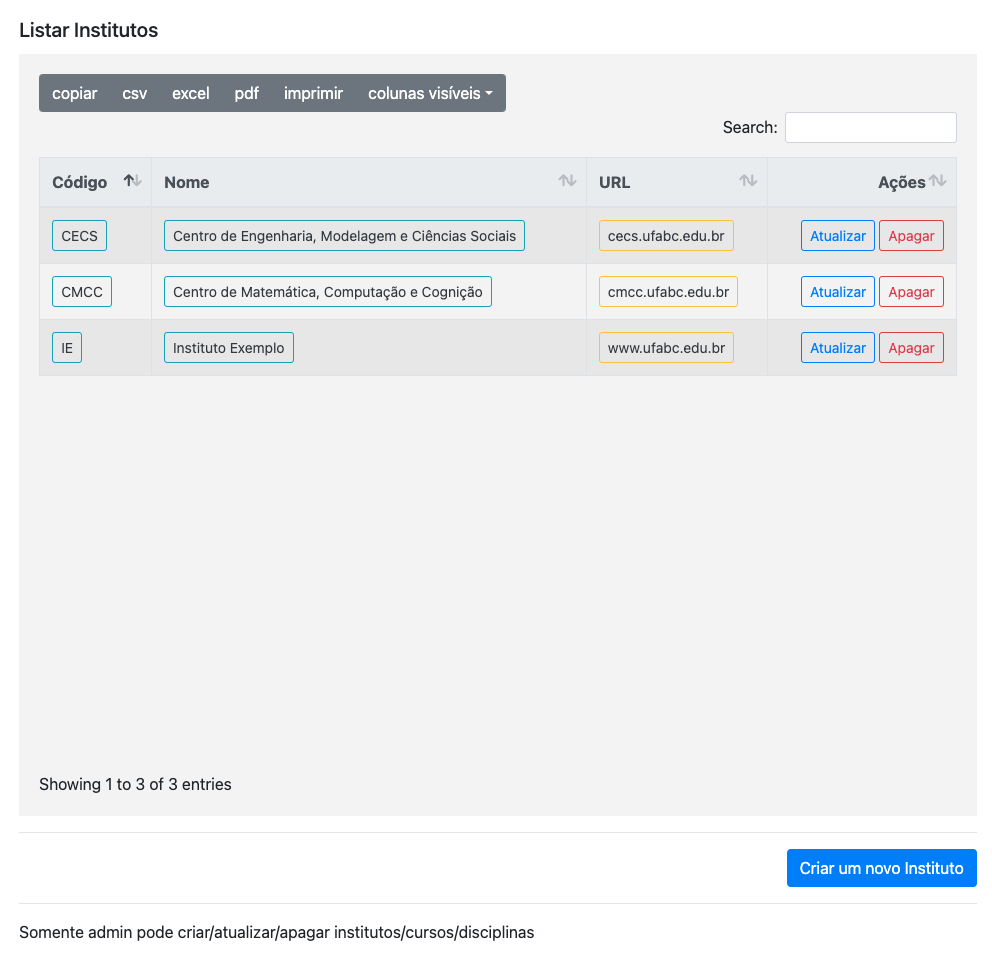
\includegraphics[width=0.9\textwidth]{cap03_figInstituto2.png}
  \caption{Tela com a lista de institutos vista pelo administrador, que pode atualizar, apagar ou criar um instituto para simular um curso pertencer aos institutos CECS e CMCC.}
  \label{fig:cap03_instituicao2}
\end{figure}

\begin{figure}[!ht]
  \centering
  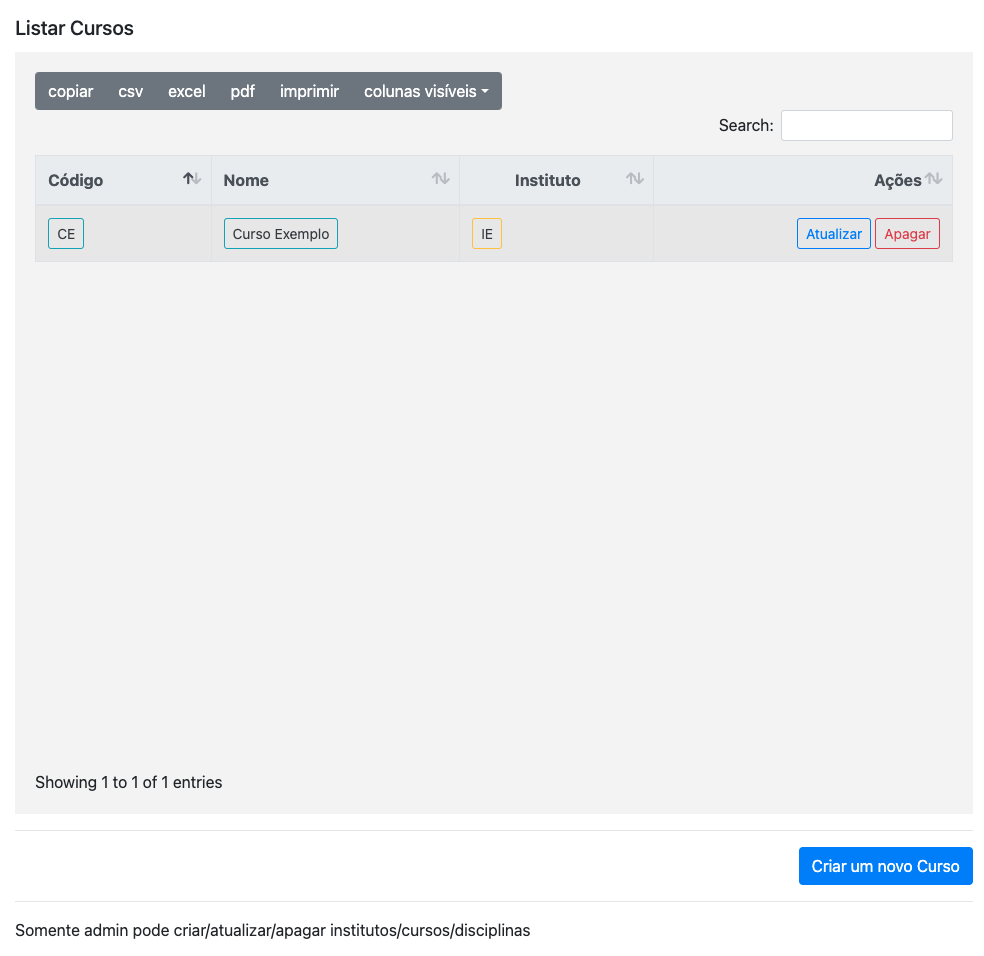
\includegraphics[width=0.9\textwidth]{cap03_figCursoListar2.png}
  \caption{Tela com a lista de curso, vista pelo administrador.}
  \label{fig:cap03_figCursoListar2}
\end{figure}

\begin{figure}[!ht]
  \centering
  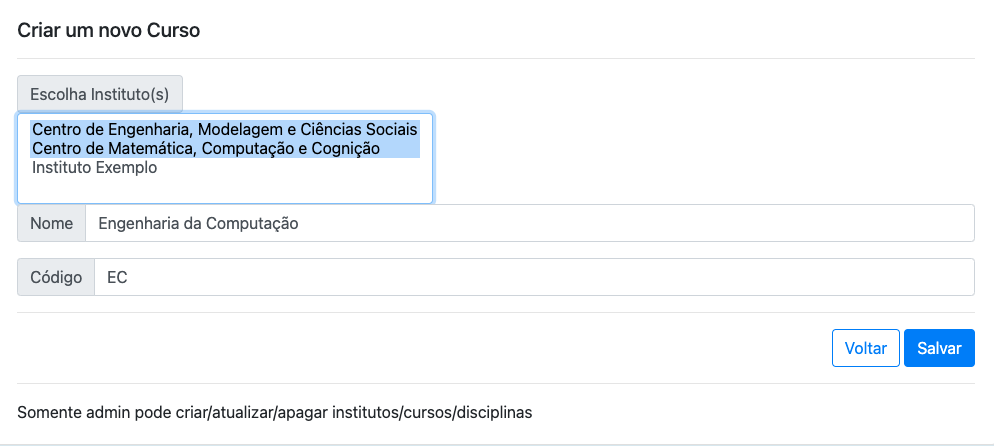
\includegraphics[width=0.9\textwidth]{cap03_figCursoCria2.png}
  \caption{Tela para o administrador criar um curso novo relacionado a dois institutos. Manter a tecla ``Ctrl'' pressionada para escolher mais de uma opção.}
  \label{fig:cap03_cursoCria2}
\end{figure}

\begin{figure}[!ht]
  \centering
  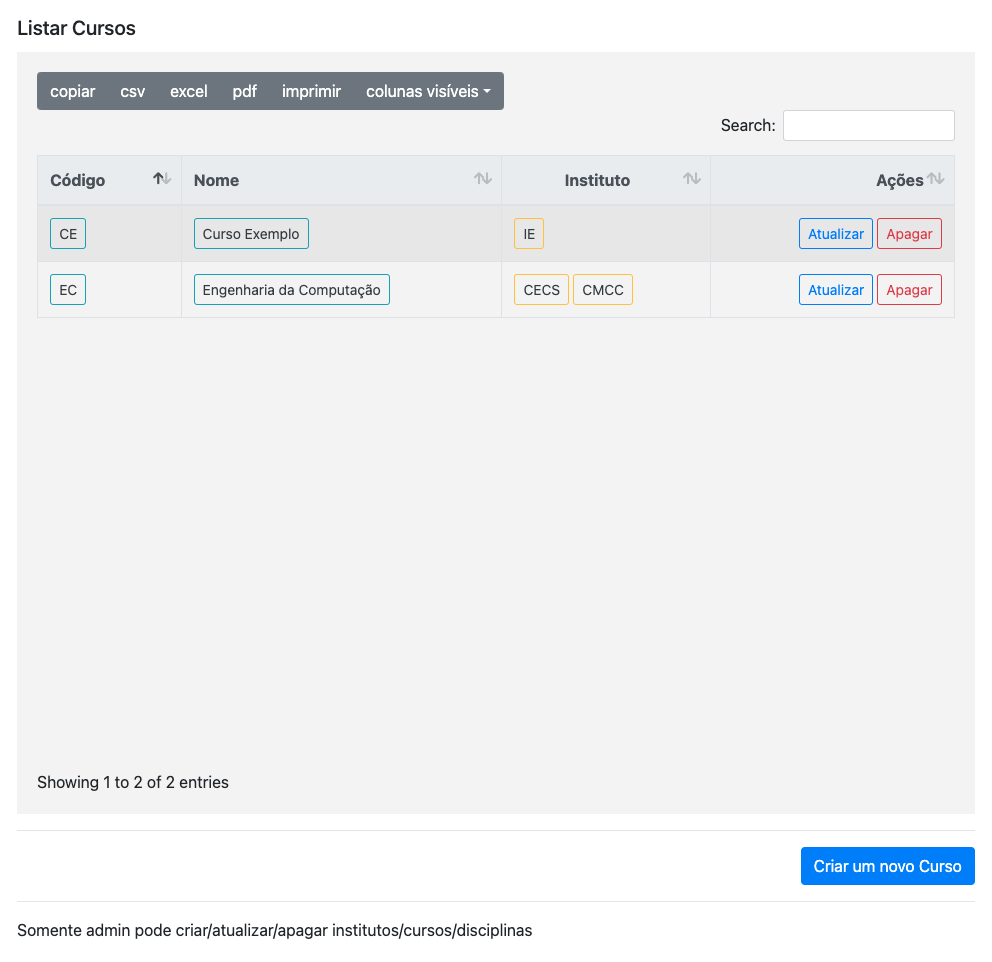
\includegraphics[width=0.9\textwidth]{cap03_figCursoListar3.png}
  \caption{Tela com a lista de curso, vista pelo  administrador, após ter criado o curso Engenharia da Computação na Figura \ref{fig:cap03_cursoCria2}.}
  \label{fig:cap03_figCursoListar3}
\end{figure}

\subsection{Criar uma disciplina relacionada a dois cursos}

Nas Seções \ref{sec:curso} -- \nameref{sec:curso} e \ref{sec:disciplina} -- \nameref{sec:disciplina}, foram abordados os procedimentos para o administrador poder criar cursos e disciplinas, respectivamente. Para ilustrar a relevância da criação de uma disciplina relacionada a dois cursos, será apresentado o seguinte cenário.

A disciplina de Processamento Digital de Imagens (PDI) é uma área da Ciência da Computação que se dedica ao estudo e desenvolvimento de técnicas e algoritmos para manipulação, análise e PDI. Essa disciplina é muito importante tanto para estudantes de graduação em Ciência da Computação quanto para estudantes de mestrado e doutorado, por oferecer uma base sólida de conhecimentos e habilidades para a solução de problemas em diversas áreas de aplicação.

No curso de graduação em Ciência da Computação, a disciplina de PDI aborda diversas técnicas relevantes para o processamento e análise de imagens digitais. Entre elas, destaca-se a representação de imagens digitais, que envolve o uso de matrizes para representar as cores dos pixels, e técnicas de filtragem, que permitem a melhoria da qualidade da imagem, através da redução de ruídos e realce de contornos de objetos.

Além disso, a disciplina de PDI também aborda técnicas de segmentação de imagens, que permitem a identificação de regiões de interesse na imagem, e técnicas de reconhecimento de padrões em imagens, que permitem a identificação de objetos, faces e outros elementos na imagem.

Durante o curso de mestrado ou doutorado em Ciência da Computação, a disciplina de PDI explora técnicas avançadas, incluindo o uso de Redes Neurais Convolucionais (CNN -- do inglês \textit{Convolutional Neural Network}). Essas técnicas têm se mostrado altamente eficazes para a segmentação, reconhecimento e classificação de imagens.

As CNN são uma classe de Redes Neurais Artificiais que têm sido amplamente utilizadas em tarefas de PDI, como a segmentação de objetos em imagens médicas ou a classificação de imagens em categorias específicas. Essas redes podem extrair características das imagens de forma automática, sem a necessidade de recursos humanos para a extração manual de características.

Com a utilização de CNN, é possível obter excelentes resultados na segmentação, reconhecimento e classificação de imagens. Por exemplo, na área médica, é possível identificar automaticamente regiões de interesse em imagens de ressonância magnética ou tomografia computadorizada, auxiliando no diagnóstico de doenças.

Portanto, a disciplina de PDI é de grande importância tanto para os estudantes de graduação quanto para os estudantes de mestrado e doutorado em Ciência da Computação. Além disso, as questões relacionadas a essa disciplina podem ser compartilhadas entre esses dois cursos.

Dessa forma, é viável adicionar a disciplina de PDI no MCTest e relacioná-la com os cursos de graduação e pós-graduação, conforme ilustrado na Figura \ref{fig:cap03_figDisciplina2}. Esse processo é semelhante ao de associar um curso a dois institutos.

\begin{figure}[!ht]
  \centering
  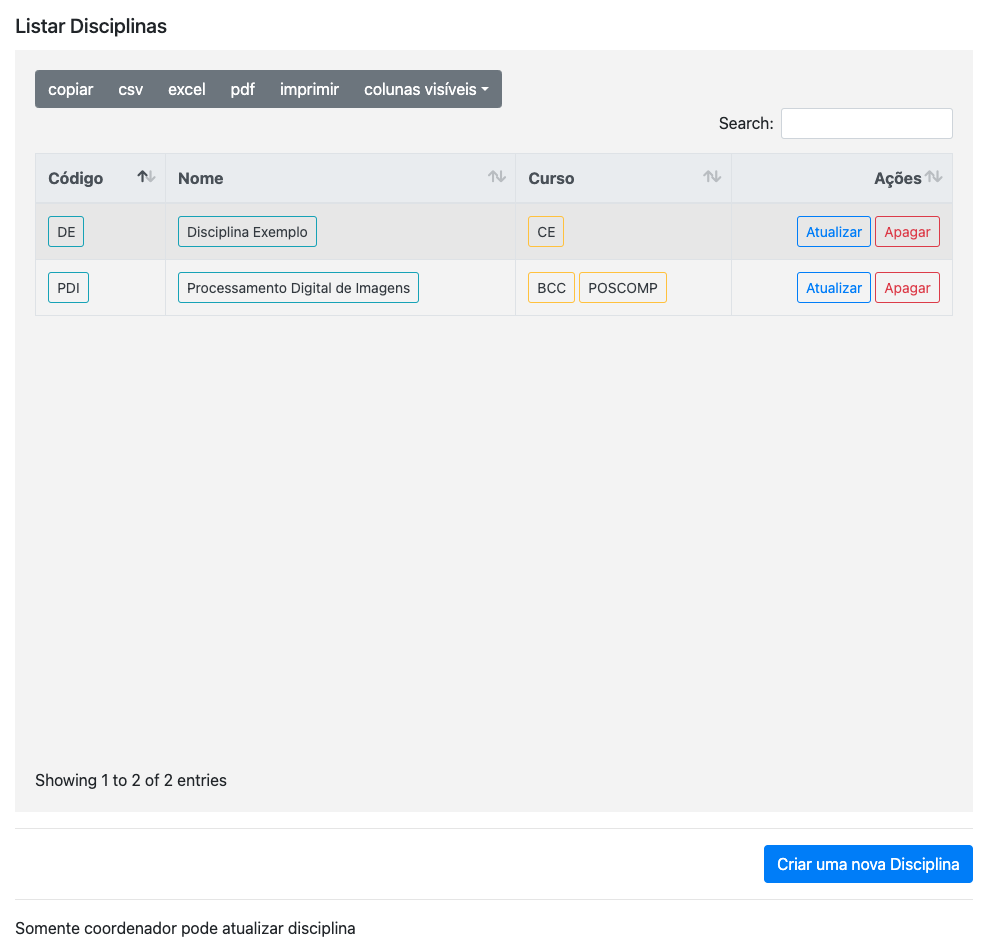
\includegraphics[width=0.9\textwidth]{cap03_figDisciplina2.png}
  \caption{Tela com a lista de disciplinas, vista pelo  administrador, com destaque para a disciplina PDI, que está relacionada aos cursos de BCC e POSCOMP.}
  \label{fig:cap03_figDisciplina2}
\end{figure}

\subsection{Acesso ao banco de dados}

Embora o administrador tenha acesso direto ao banco de dados (BD) ao pressionar o botão ``Admin'' na Figura \ref{fig:cap2_navegacao}-(e), a melhor opção é evitar alterar o BD usando esse recurso. É recomendado utilizar as telas de navegação do MCTest para fazer as alterações necessárias, pois alterar o BD diretamente pode resultar em relacionamentos incorretos entre as entidades, o que pode tornar o sistema inoperante. %Para aqueles que desejam obter detalhes sobre a arquitetura de software e o banco de dados desenvolvido no MCTest, recomendamos consultar a Parte \ref{part:topicosAvancados} deste livro.

\begin{figure}[!ht]
  \centering
  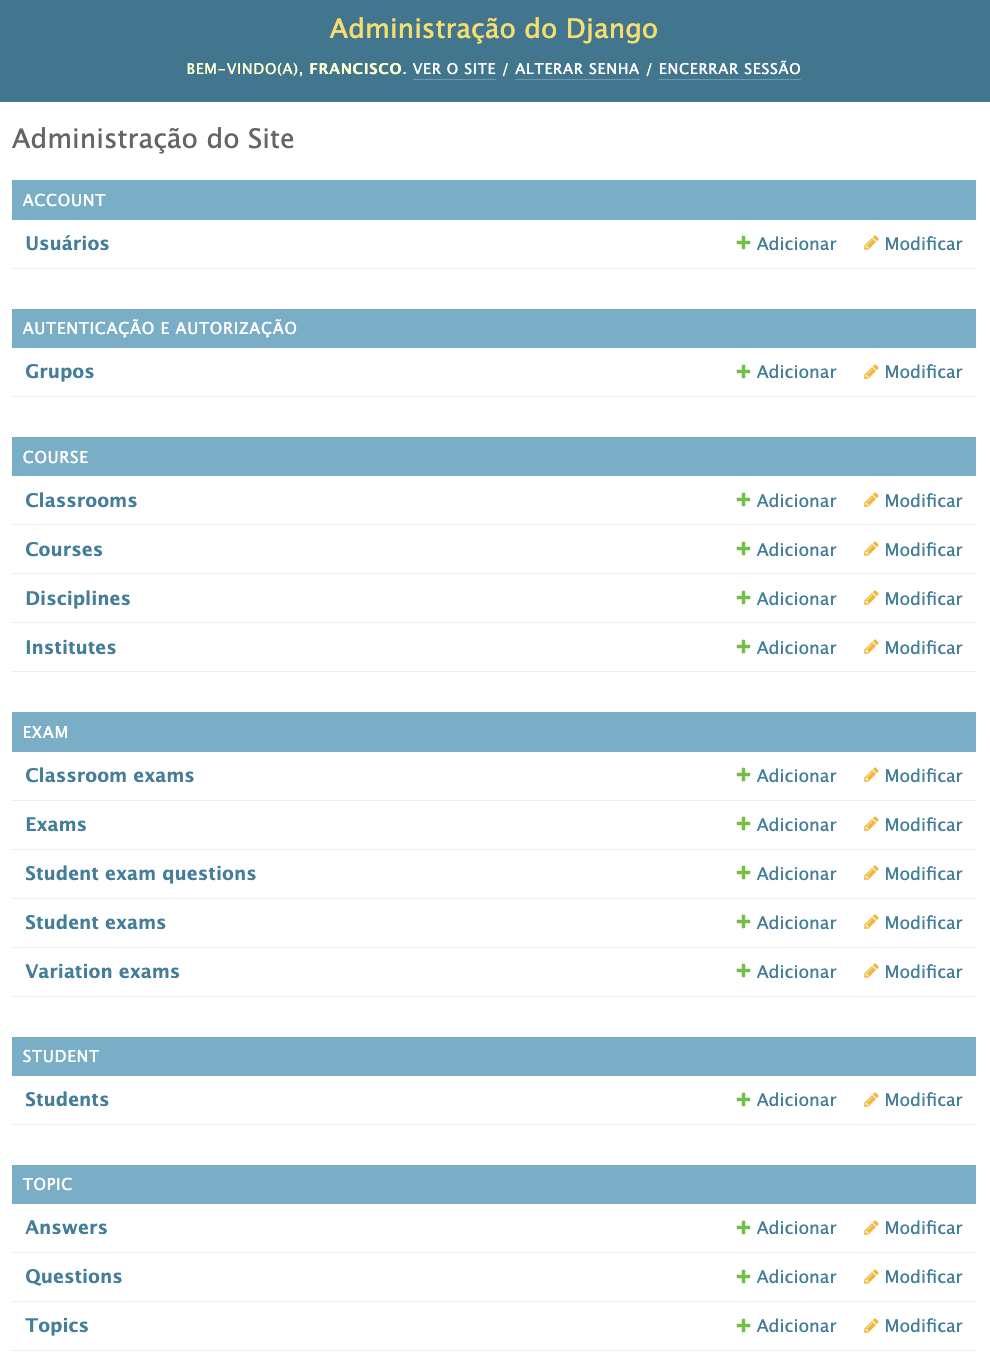
\includegraphics[width=0.85\textwidth]{cap03_figAdminBD.png}
  \caption{Tela com a lista de entidades que o administrador pode fazer manutenção diretamente no BD.}
  \label{fig:cap03_figAdminBD}
\end{figure}


\section{Coordenador}

Nesta seção, serão abordadas as funcionalidades destinadas ao coordenador de disciplina, que envolvem a manutenção de tópicos e disciplinas. O coordenador tem a responsabilidade de criar e gerenciar os tópicos e disciplinas que serão utilizados pelos professores para criar exames e Exercícios de Programação (EPs).

\subsection{Criar um tópico relacionado a duas ou mais disciplinas}

A interdisciplinaridade é uma abordagem essencial na educação moderna, que visa integrar conhecimentos de diferentes áreas para enriquecer o processo de aprendizagem e formação dos estudantes. Nesse sentido, a UFABC se destaca na interdisciplinaridade, conforme apresentado em sua missão:

\begin{mybox}{green}{\textbf{Missão da UFABC:\\\vspace{-3mm}\hrule}}
\begin{quote}
    \textit{Promover o avanço do conhecimento por ações de ensino, pesquisa e extensão, tendo como fundamentos básicos a interdisciplinaridade, a excelência e a inclusão social.}
\end{quote}
\end{mybox}

Nesse sentido, compartilhar um tópico entre duas ou mais disciplinas pode trazer inúmeros benefícios para a educação. Como mencionado na Seção \ref{sec:topicos} -- \nameref{sec:topicos}, um tópico só existe no MCTest se pertencer a uma disciplina, mas pode ser compartilhado entre várias delas. Além disso, as questões só existem se estiverem inseridas em um tópico. 

Um exemplo prático dessa abordagem pode ser observado na UFABC, na qual a lógica de programação é abordada em diversas disciplinas. Especificamente, esse tópico é tratado no Bacharelado em Ciência e Tecnologia (BCT), no segundo exame da disciplina de Bases Computacionais da Ciência (CS0) para os ingressantes e no primeiro exame de Processamento da Informação (PI -- CS1) no terceiro quadrimestre dos ingressantes. Atualmente, a maioria das turmas dessas duas disciplinas utiliza a linguagem Python. Além disso, a disciplina de Programação Estruturada (PE -- CS2), oferecida no Bacharelado em Ciência da Computação, também trata da lógica de programação no primeiro exame, utilizando a linguagem C.

Ao elaborar questões sobre lógica de programação de forma independente da linguagem utilizada, é possível compartilhar essas questões entre as três disciplinas mencionadas. Essa prática tem várias vantagens:

\begin{description}
\item[Otimização de recursos:] Ao compartilhar questões e tópicos, é possível economizar tempo e esforço dos professores na criação de materiais didáticos, permitindo que se concentrem em outras tarefas importantes, como atendimento aos estudantes e pesquisas de novas metodologias de ensino;

\item[Consistência no conteúdo:] Ao utilizar tópicos comuns entre diferentes disciplinas, os estudantes são expostos a uma abordagem consistente e coerente, facilitando a compreensão e a conexão entre os conceitos aprendidos;

\item[Desenvolvimento de habilidades transferíveis:] Ao aprender sobre um tópico em várias disciplinas, os estudantes têm a oportunidade de desenvolver habilidades transferíveis, como pensamento crítico, resolução de problemas e comunicação. Essas habilidades são essenciais para o sucesso em diversas áreas profissionais;

\item[Fomento da interdisciplinaridade:] Compartilhar tópicos entre disciplinas incentiva os estudantes a estabelecer conexões entre diferentes campos do conhecimento, promovendo uma educação mais integrada e abrangente.
\end{description}

A Figura \ref{fig:cap03_figTopico2} exemplifica uma lista de tópicos, demonstrando que um determinado tópico pode pertencer a três disciplinas diferentes. Adicionalmente, a Figura \ref{fig:cap03_figDisciplina3} apresenta detalhes específicos da disciplina de Processamento da Informação, com destaque para os tópicos compartilhados. Essa configuração permite que um professor utilize todas as questões desses tópicos ao elaborar um exame.

\begin{figure}[!ht]
  \centering
  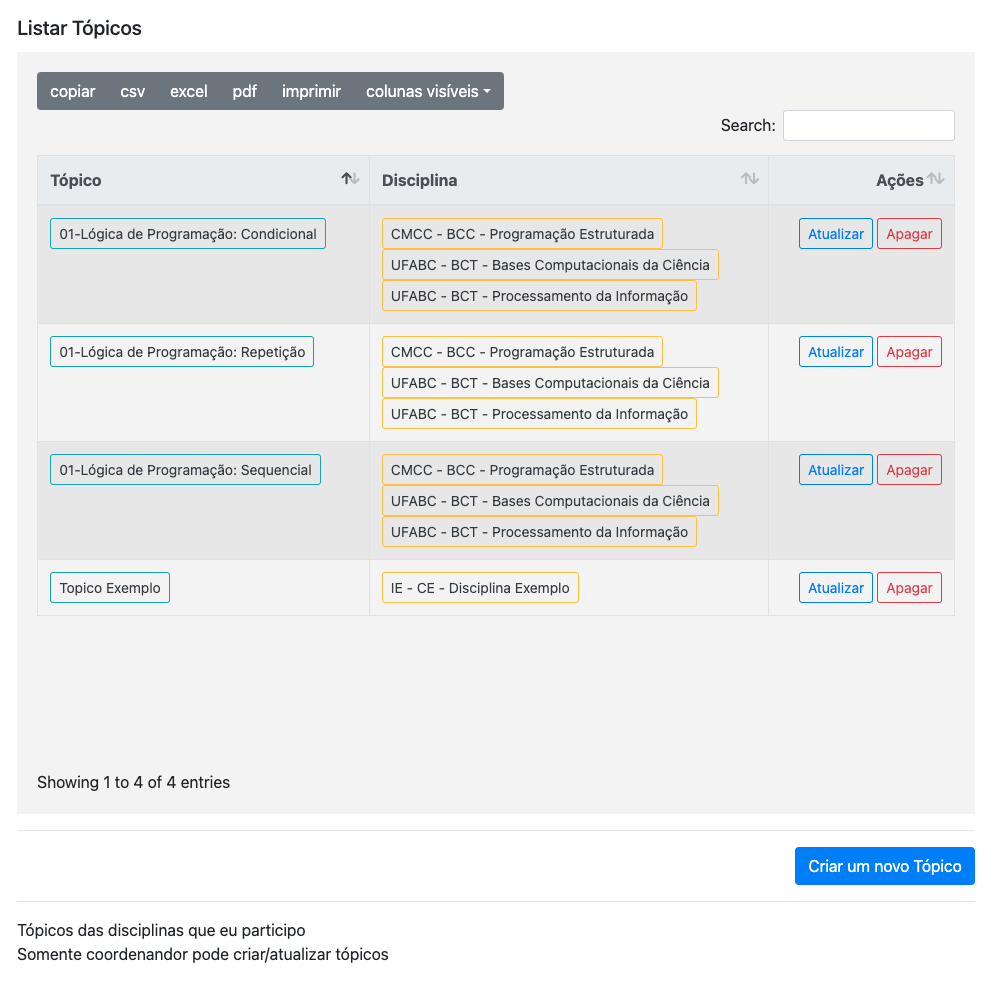
\includegraphics[width=0.9\textwidth]{cap03_figTopico2.png}
  \caption{Tela com a lista de tópicos, vista pelo  coordenador. É possível observar o compartilhamento de tópicos entre disciplinas.}
  \label{fig:cap03_figTopico2}
\end{figure}

\begin{figure}[!ht]
  \centering
  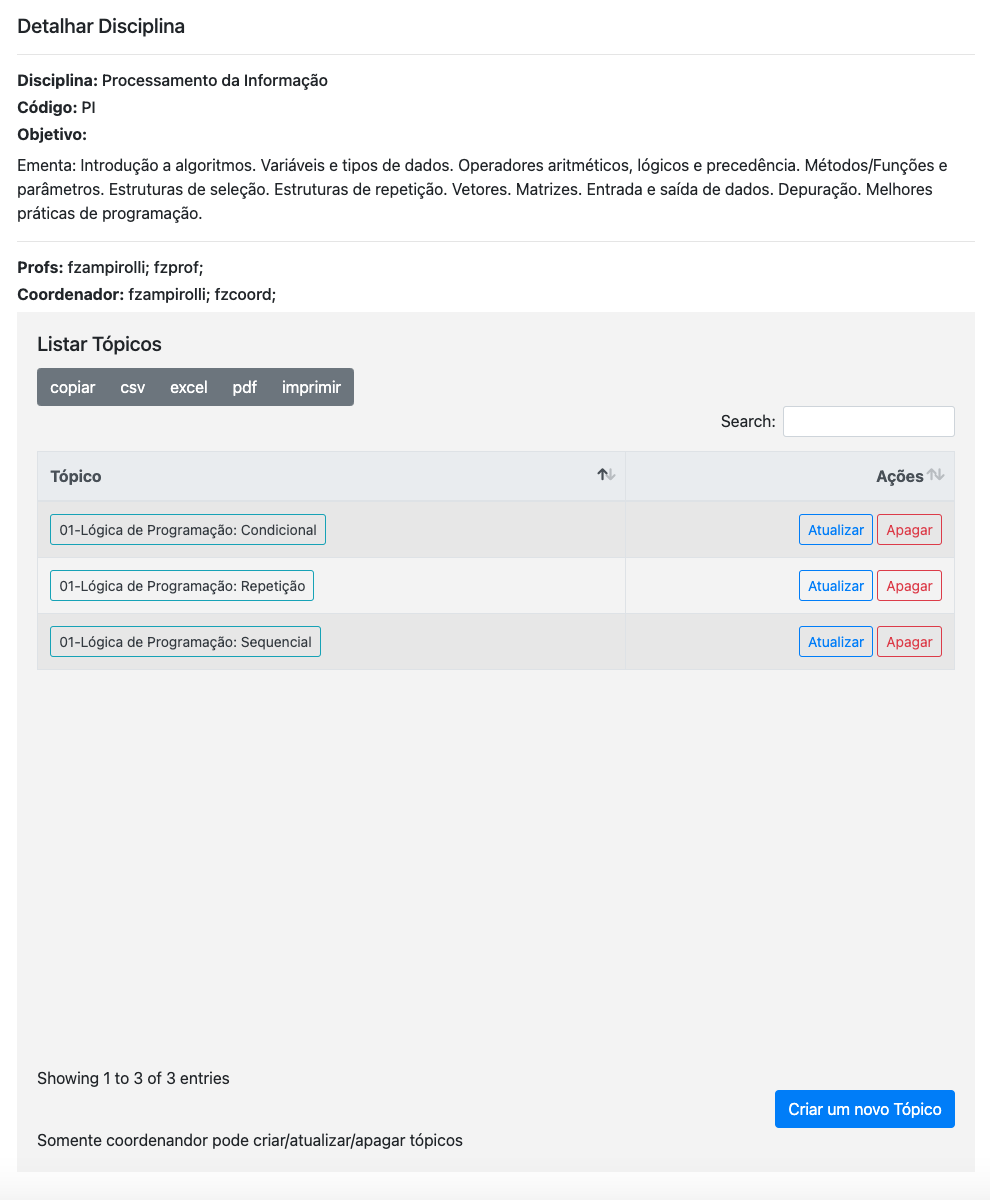
\includegraphics[width=0.9\textwidth]{cap03_figDisciplina3.png}
  \caption{Tela com detalhes da disciplina de Processamento da Informação, vista pelo  coordenador, com os tópicos compartilhados também apresentados na Figura \ref{fig:cap03_figTopico2}.}
  \label{fig:cap03_figDisciplina3}
\end{figure}


\subsection{Criar várias turmas com arquivo CSV}\label{sec:variasTurmasCSV}

No capítulo anterior, foi abordada a criação de disciplinas na Seção \ref{sec:disciplina} -- \nameref{sec:disciplina}, e a criação de turmas com estudantes foi apresentada na Seção \ref{sec:turma} -- \nameref{sec:turma}. No entanto, em algumas situações, pode ser necessário criar várias turmas da mesma disciplina simultaneamente. Para atender a essa demanda, foram implementadas funcionalidades que permitem ao coordenador cadastrar todos os professores e estudantes de múltiplas turmas de uma só vez, por meio da importação de arquivos no formato CSV, conforme ilustrado na Figura \ref{fig:cap03_figDisciplinaAtualiza22}.

\begin{mybox}{pink}{\textbf{Melhorias:\\\vspace{-3mm}\hrule\vspace{3mm}}}
É importante ressaltar que esse recurso precisa ser aprimorado e, por enquanto, o botão ``Upload-Turma'' irá remover todos os estudantes de todas as turmas associadas a essa disciplina, atualizando com os novos dados do arquivo CSV. Portanto, é fundamental ter cuidado ao utilizar essa funcionalidade e garantir que os dados do arquivo CSV estejam corretos e atualizados.
\end{mybox}

%Essa funcionalidade é extremamente útil para facilitar o cadastro de muitos estudantes e professores de uma só vez, além de permitir que os dados sejam atualizados de forma mais eficiente. No entanto, é importante lembrar que a precisão e a consistência dos dados do arquivo CSV são fundamentais para a realização de exames precisos e eficazes.

\begin{figure}[!ht]
  \centering
  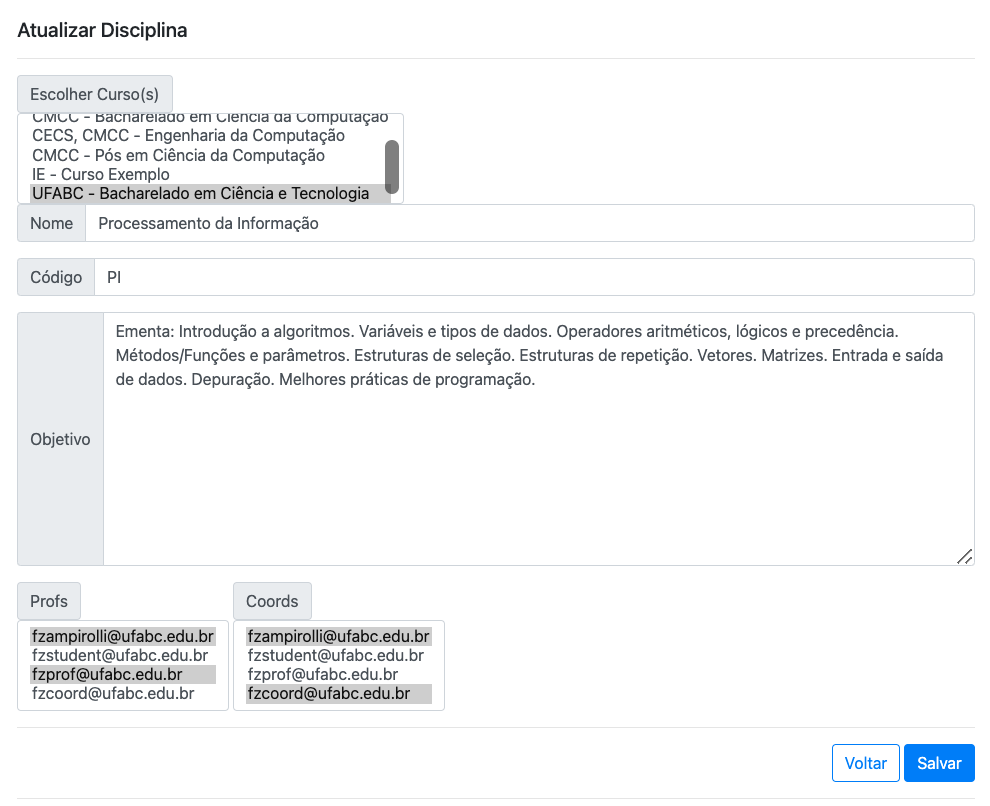
\includegraphics[width=0.9\textwidth]{cap03_figDisciplinaAtualiza2a.png}
  \caption{(Parte 1) Tela de criação da disciplina de Processamento da Informação pelo administrador.}
  \label{fig:cap03_figDisciplinaAtualiza2a}
\end{figure}

\begin{figure}[!ht]
  \centering
  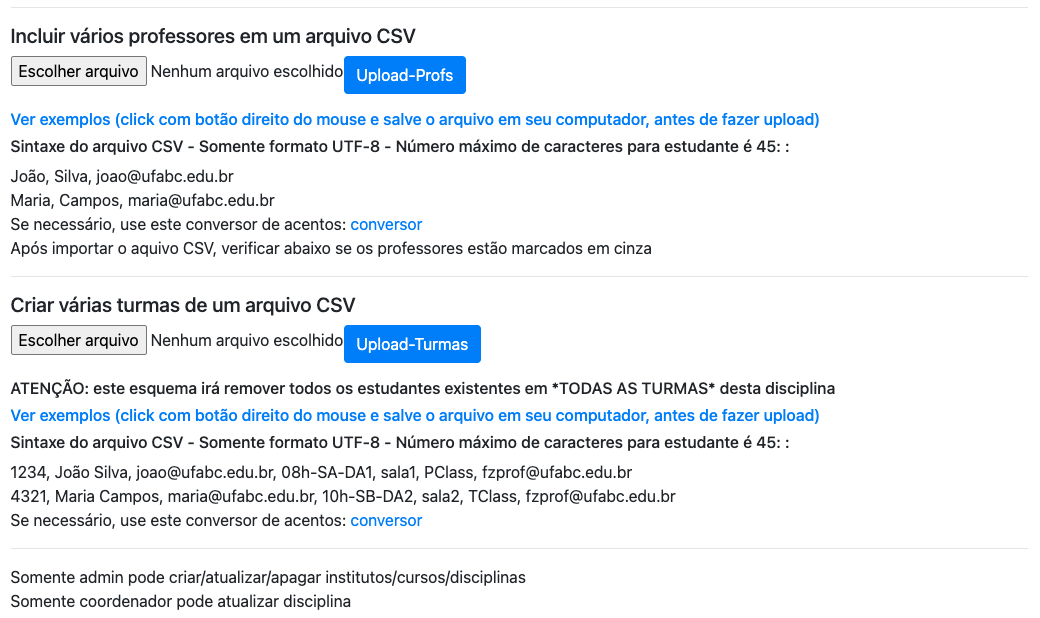
\includegraphics[width=0.9\textwidth]{cap03_figDisciplinaAtualiza22.png}
  \caption{(Parte 2) Tela de criação da disciplina de Processamento da Informação pelo administrador. É possível incluir professores, turmas e estudantes pela importação de dois arquivos no formato CSV.}
  \label{fig:cap03_figDisciplinaAtualiza22}
\end{figure}

As telas para criação e atualização de disciplinas apresentadas nas Figuras \ref{fig:cap03_figDisciplinaAtualiza2a} e \ref{fig:cap03_figDisciplinaAtualiza22} são semelhantes e estão disponíveis tanto para o administrador quanto para o coordenador da disciplina. 
Na Figura \ref{fig:cap03_figDisciplinaAtualiza22}, o primeiro arquivo CSV é destinado ao coordenador para inserir diversos professores na disciplina, com o perfil de professor já configurado, como apresentado a seguir:
\begin{myboxCode}{corCSV}{\textbf{Arquivo CSV com dados dos professores:}}\vspace{3mm}
\hrule
\begin{verbatim}
João, da Silva, joao@ufabc.edu.br
Maria, Gonçalves, maria@ufabc.edu.br
\end{verbatim}
\end{myboxCode}

Por sua vez, o segundo arquivo CSV nesta figura é utilizado pelo coordenador para adicionar várias turmas, contendo estudantes e professores, com um formato pré-definido como segue:
\begin{myboxCode}{corCSV}{\textbf{Arquivo CSV com dados de estudantes e professores:}}\vspace{3mm}
\hrule
\begin{verbatim}
123, João Silva, js@gmail.com, DA1, sala1, PClass, fzprof@ufabc.edu.br
987, Maria Campos, mc@gmail.com, DA2, sala2, TClass, fzprof@ufabc.edu.br
\end{verbatim}
\end{myboxCode}

Este último arquivo CSV apresenta as seguintes colunas, em ordem: identificação do estudante, nome completo do estudante, e-mail do estudante, turma, sala, ``PClass'' (para turma prática) ou ``TClass'' (para turma teórica) e e-mail do professor.


\section{Professor} \label{sec:professor}

Nesta seção será abordada mais funcionalidades destinadas aos professores, que incluem a manutenção de turmas, questões e exames. O professor é responsável por criar as turmas, selecionar as questões e criar os exames para avaliar os estudantes. Com o sistema MCTest, os professores podem criar exames com questões de múltipla escolha (QMs) ou dissertativas (QTs), incluindo EPs parametrizados para correção automática no Moodle, utilizando o \textit{plugin} VPL.

\subsection{Criar turma com arquivo CSV}\label{sec:professorCriarTurma}

O professor é responsável por criar uma turma e manter os dados de seus estudantes atualizados, como discutido na Seção \ref{sec:turma} -- \nameref{sec:turma}. O primeiro passo é criar a turma e relacioná-la a uma disciplina, conforme ilustrado na Figura \ref{fig:cap02_figTurmaCriar}. Em seguida, o professor pode inserir os estudantes de três maneiras distintas:

\begin{enumerate}
    \item  Selecionando vários estudantes na lista com a tecla ``Ctrl'' pressionada, como demonstrado na Figura \ref{fig:cap02_figTurmaAtualiza};
    \item Incluindo um estudante de cada vez, conforme exemplificado na Figura \ref{fig:cap02_figTurmaAtualiza2} e/ou atualizando os dados de um estudante, como demonstrado na Figura \ref{fig:cap02_figTurmaAtualiza3}; 
    \item Ou, de maneira mais eficiente, utilizando um arquivo CSV, vistos a seguir.
\end{enumerate}

Para utilizar um arquivo CSV para preencher uma turma com estudantes, o professor deve primeiro criar a turma, como ilustrado na Figura \ref{fig:cap02_figTurmaCriar}, e em seguida fazer o \textit{upload} do arquivo no início da Figura \ref{fig:cap02_figTurmaAtualiza}, selecionando o arquivo em ``Escolher arquivo'' e, em seguida, clicando no botão ``Importar-Estudantes''. O arquivo deve seguir o formato apresentado abaixo:

\begin{myboxCode}{corCSV}{\textbf{Arquivo CSV com dados completos:}}\vspace{3mm}
\hrule
\begin{verbatim}
123, João da Silva, joao@aluno.ufabc.edu.br
987, Maria Gonçalves, maria@aluno.ufabc.edu.br
\end{verbatim}
\end{myboxCode}

Observe que a primeira linha do arquivo já representa o primeiro estudante, com sua identificação, nome completo e e-mail, separados por vírgula ou ponto e vírgula. É importante destacar que o e-mail é opcional, como no exemplo abaixo:

\begin{myboxCode}{corCSV}{\textbf{Arquivo CSV, sem e-mail: }}\vspace{3mm}
\hrule
\begin{verbatim}
123, João da Silva
987, Maria Gonçalves
\end{verbatim}
\end{myboxCode}

\subsection{Criar turma com arquivo CSV -- restrições}\label{sec:professorCriarTurma2}

O professor deve ter uma atenção especial aos acentos e símbolos especiais neste arquivo CSV, que deve seguir o formato \texttt{UTF-8}. Uma alternativa é converter esses símbolos para o formato \LaTeX{}, utilizando, por exemplo, o recurso disponível na internet em \href{https://w2.syronex.com/jmr/latex-symbols-converter}{w2.syronex.com/jmr/latex-symbols-converter}, conforme exemplo abaixo:

\begin{myboxCode}{corCSV}{\textbf{Arquivo CSV, com acentos no formato \LaTeX: }}\vspace{3mm}
\hrule
\begin{verbatim}
123, Jo\~{a}o da Silva, joao@aluno.ufabc.edu.br
987, Maria Gon\c{c}alves, maria@aluno.ufabc.edu.br
\end{verbatim}
\end{myboxCode}

\begin{mybox}{corObs}{\textbf{Observações:\\\vspace{-3mm}\hrule\vspace{1mm}}}
\begin{enumerate}
    \item O nome do estudante no sistema tem um limite de 45 caracteres. Caso o arquivo CSV contenha um nome de estudante com mais de 45 caracteres, o sistema irá remover automaticamente o(s) sobrenome(s) do meio, de trás para frente, mantendo o último sobrenome, até atingir os 45 caracteres permitidos. Essa medida é tomada para garantir a integridade dos dados e evitar problemas de exceder o limite de caracteres ao incluir o nome do estudante em um exame. Um exemplo pode ser visto na Figura \ref{fig:cap03_figTurmaCSV};
    \item Caso o arquivo contenha um identificador já existente, o sistema não criará ou alterará o mesmo.
\end{enumerate}
\end{mybox}

\begin{figure}[!ht]
  \centering
  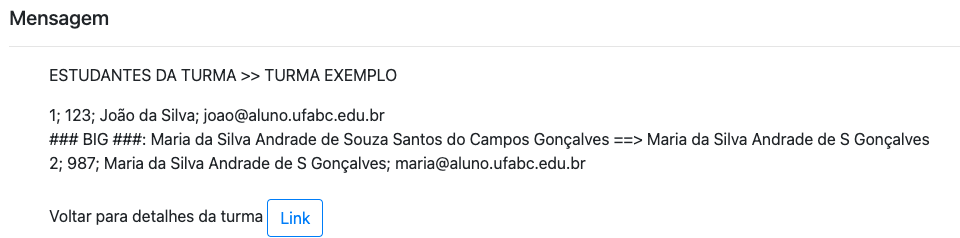
\includegraphics[width=0.9\textwidth]{cap03_figTurmaCSV.png}
  \caption{Tela mostrando o resultado do cadastro de estudantes utilizando a importação de um arquivo no formato CSV.}
  \label{fig:cap03_figTurmaCSV}
\end{figure}

\section{Considerações finais}

Este capítulo expandiu as funcionalidades apresentadas no capítulo anterior, apresentando recursos avançados disponíveis no MCTest para usuários com diferentes papéis (administrador, coordenador e professor). Cada tipo de usuário tem acesso a um conjunto específico de ferramentas para criar e gerenciar as diversas entidades do sistema de avaliação, como institutos, cursos, disciplinas, tópicos, turmas, professores e estudantes.

As funcionalidades abordadas procuram facilitar o gerenciamento das entidades e a configuração do sistema conforme as necessidades de cada instituição. O administrador, em particular, tem permissões amplas para configurar o sistema e gerenciar o acesso dos usuários. Os coordenadores são responsáveis por gerenciar disciplinas, tópicos e turmas. Já os professores podem gerenciar questões, exames, turmas e estudantes sob sua responsabilidade.

Nos próximos capítulos da Parte \ref{part:questoesMCTest}, serão abordados a criação e o gerenciamento de questões no MCTest, com foco nas diversas formas de elaboração, revisão e aprovação das questões destinadas a serem aplicadas nos exames discutidos na Parte \ref{part:exames}.\cleardoublepage

%%%%%%%%%%%%%%%%%%%%%%%%%%%%%%%%%%%%%%%%%%%%%%%%%%%%%%%
\part{Questões no MCTest}\label{part:questoesMCTest}\cleardoublepage
%%%%%%%%%%%%%%%%%%%%%%%%%%%%%%%%%%%%%%%%%%%%%%%%%%%%%
\mychapter{Questões estáticas}\label{ch:questoesClassicasMCTest}

A criação de questões estáticas é fundamental para a avaliação educacional e existem diversas abordagens e formatos disponíveis. Neste capítulo, serão abordados os dois principais tipos de questões estáticas utilizados em avaliações educacionais: as questões de múltipla escolha (QMs) e as questões dissertativas ou de texto (QTs). O objetivo é apresentar as características e particularidades de cada tipo de questão, bem como as vantagens e desvantagens de sua utilização na avaliação da aprendizagem. É importante destacar que as questões apresentadas neste capítulo não são parametrizadas, sendo as únicas variações os sorteios das questões e alternativas, no caso das QMs. No próximo capítulo, serão abordadas as questões parametrizadas.

Neste capítulo, será discutida a visibilidade do professor no menu do MCTest, permitindo que ele faça a manutenção das questões, exames e turmas que criou. Além disso, o professor também pode visualizar e utilizar questões criadas por outros professores cadastrados nas mesmas disciplinas.  É importante compreender como essa funcionalidade pode ser útil aos professores, proporcionando maior uniformidade e controle sobre as avaliações.

\section{Tutoriais gerais sobre a navegação de questões}\label{sec:questaoNavegacao}

Na Figura \ref{fig:cap04_figQuestao}, é apresentada a lista de questões que o usuário ``fzprof'' pode visualizar ao clicar no botão ``Questões'' à esquerda do menu superior. Esse menu exibe todas as questões criadas por todos os professores cadastrados nas mesmas disciplinas de ``fzprof''.

A Figura \ref{fig:cap04_figQuestao} exibe a lista de questões, apresentando diversos atributos (colunas), como o ``Tópico'' da disciplina, o ``Tipo'' de questão (podendo ser QM ou QT), o número de alternativas (no caso do tipo QM, que neste exemplo é cinco), o ``Grupo'' da questão (para evitar que sejam sorteadas duas ou mais questões do mesmo grupo em um exame), a dificuldade variando de 1 a 5, se é paramétrica, a identificação da questão no banco de dados (``ID''), a ``Descrição curta'' (para facilitar o entendimento do que se trata a questão sem precisar abrir todo o enunciado) e, por fim, os botões de ``Ações'', que permitem atualizar ou apagar a questão. 

\begin{figure}[!ht]
  \centering
  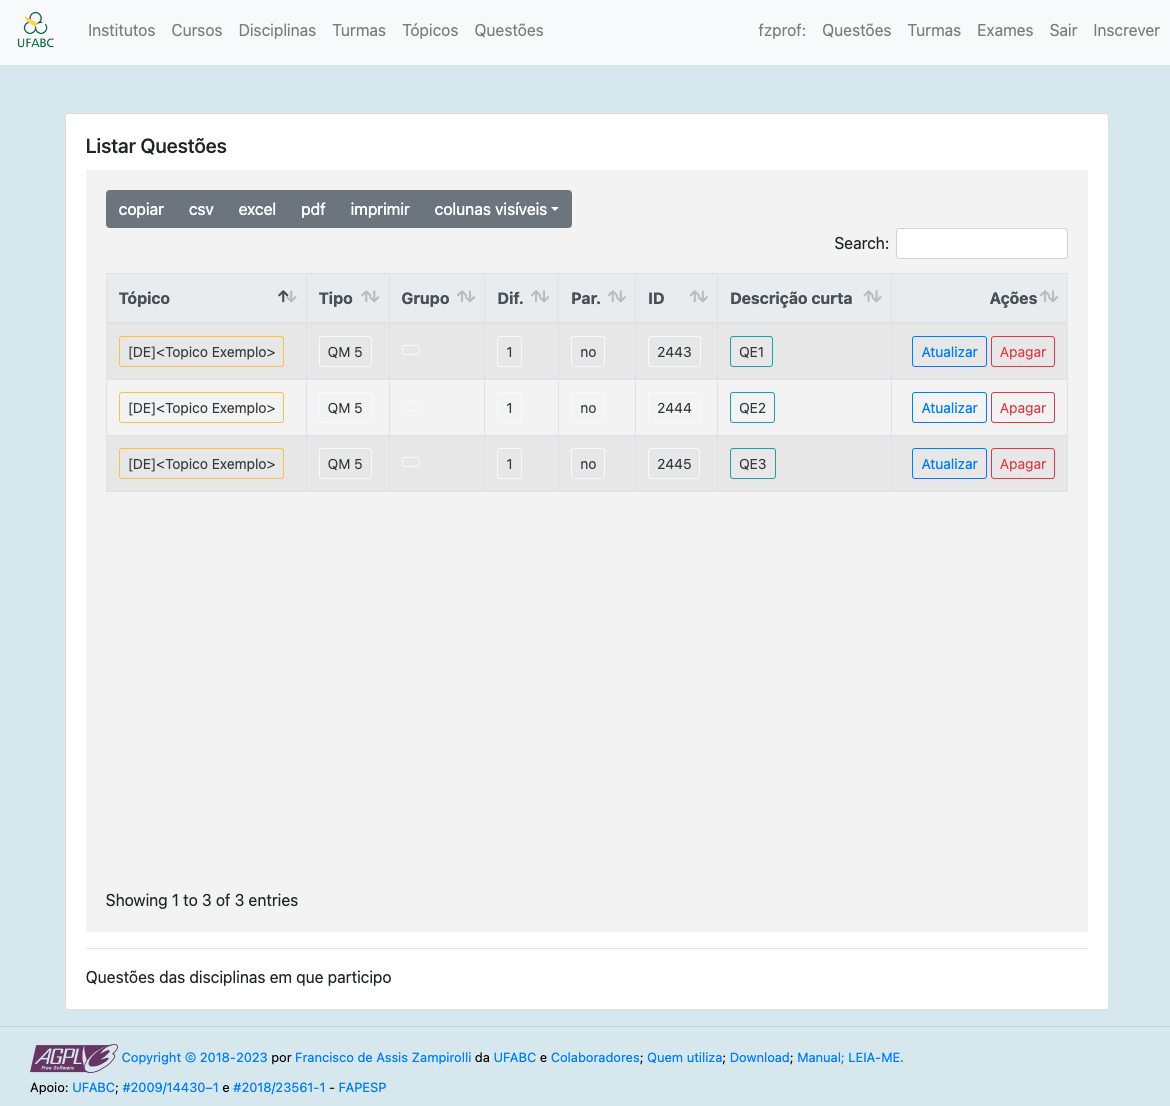
\includegraphics[width=0.9\textwidth]{cap04_figQuestao.png}
  \caption{Tela para o professor visualizar todas as questões de disciplinas que está cadastrado.}
  \label{fig:cap04_figQuestao}
\end{figure}

Caso o professor tente modificar uma questão que não é de sua autoria, será exibida a mensagem de erro apresentada na Figura \ref{fig:cap04_figQuestaoErro}.

\begin{figure}[!ht]
  \centering
  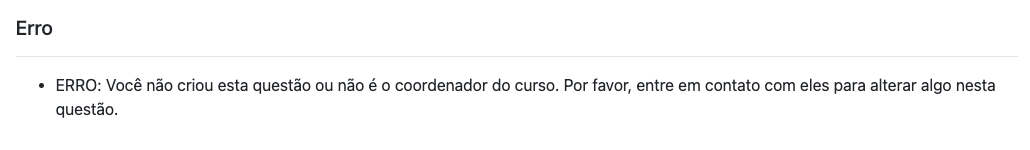
\includegraphics[width=0.9\textwidth]{cap04_figQuestaoErro.png}
  \caption{Exibição de erro ao tentar modificar questão criada por outro autor.}
  \label{fig:cap04_figQuestaoErro}
\end{figure}

\begin{mybox}{corObs}{\textbf{Observações:\\\vspace{-3mm}\hrule\vspace{1mm}}}
\begin{enumerate}
    \item Embora a Figura \ref{fig:cap04_figQuestao} exiba os botões ``Atualizar'' e ``Apagar'', é importante ressaltar que, caso o professor tente alterar ou apagar uma questão criada por outro professor, o sistema não permitirá a modificação ou exclusão da questão;
    \item É interessante manter o botão ``Atualizar'' disponível, por permitir que qualquer professor da disciplina possa visualizar como a questão foi criada. Ao clicar nas colunas ``Tipo'' até ``Descrição curta'', o professor pode conferir a questão em um modo diferente e simplificado, como mostrado na Figura \ref{fig:cap04_figQuestaoView}. É importante ressaltar que essa não é a melhor forma de visualizar os detalhes da questão, mas o professor pode acessar o PDF completo de visualização da questão clicando no botão ``Criar-PDF''.
\end{enumerate}
\end{mybox}

\begin{figure}[!ht]
  \centering
  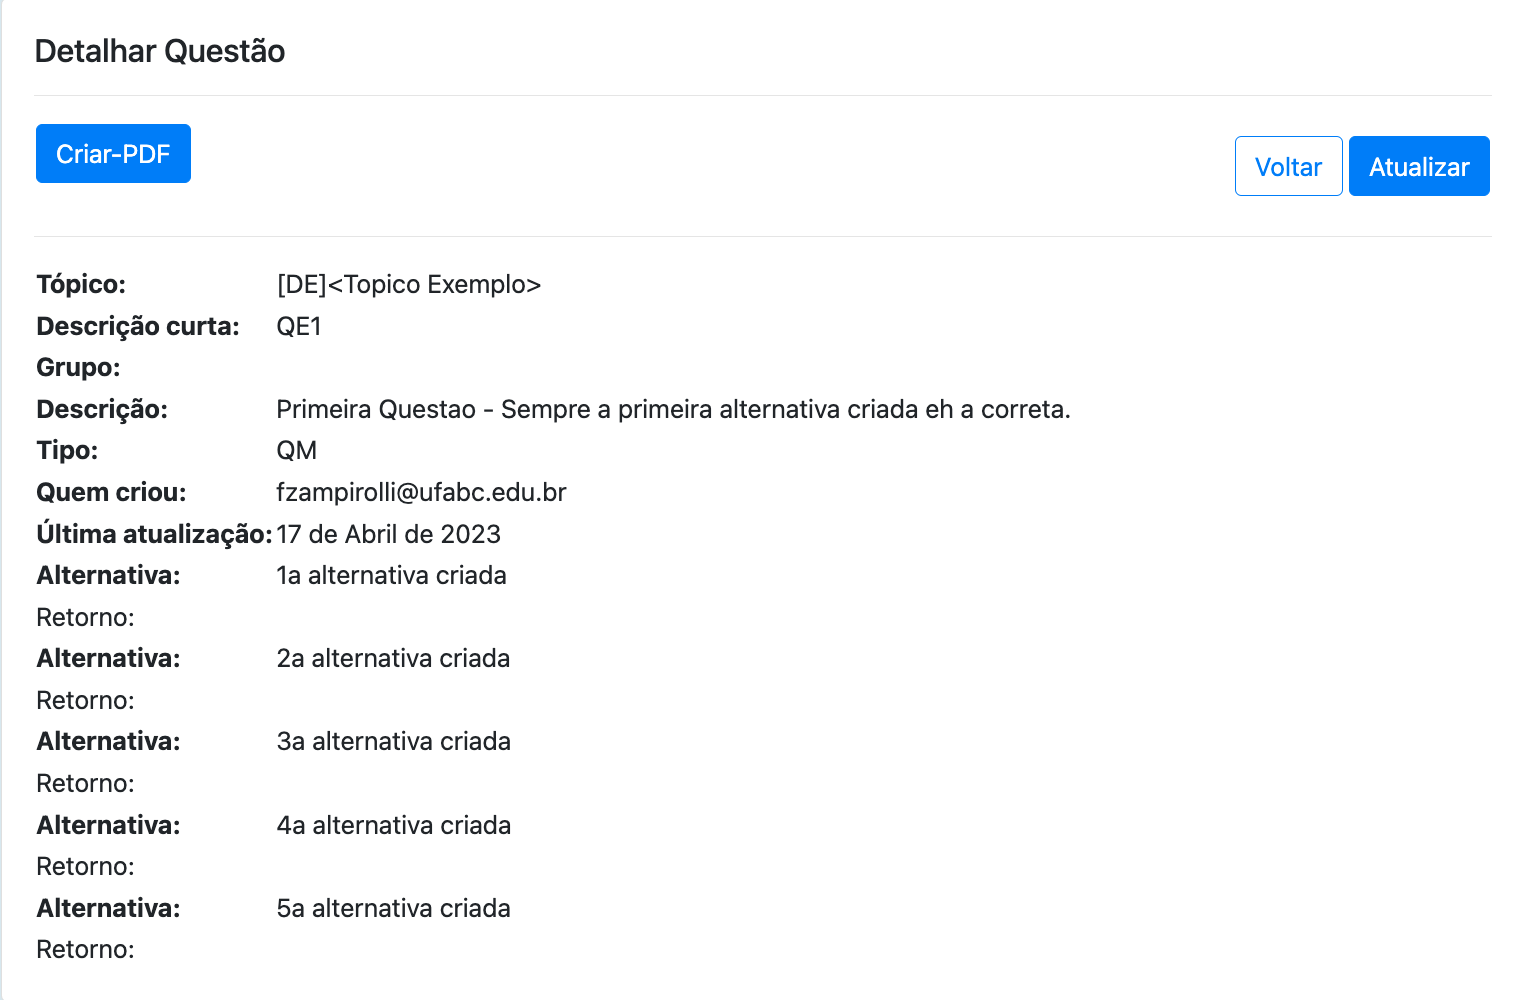
\includegraphics[width=0.9\textwidth]{cap04_figQuestaoView.png}
  \caption{Exibição da questão QE1 criada por outro autor.}
  \label{fig:cap04_figQuestaoView}
\end{figure}

Na Figura \ref{fig:cap04_figQuestaoMy}, é possível observar que o professor ``fzprof'' ainda não criou nenhuma questão. Para criar novas questões, o professor pode importar um arquivo no formato TXT, conforme exemplificado abaixo. Esse formato foi utilizado na versão 4 do MCTest, que executava no console de um computador e aceitava apenas três níveis de dificuldade: fácil (QE), médio (QM) e difícil (QH), representados em inglês por \textit{easy}, \textit{median} e \textit{hard}, respectivamente. Já a versão web atual do MCTest aceita cinco níveis de dificuldade, de 1 a 5. Ao importar uma questão de um arquivo TXT na versão web, as questões com nível de dificuldade QE terão dificuldade 1, as QM terão dificuldade 3 e as QH terão dificuldade 5.


No exemplo a seguir, o tópico é ``DE-matriz'' e é necessário existir uma disciplina com esse tópico cadastrada no MCTest. Para evitar conflitos, é recomendável incluir algum código como prefixo do tópico, como o código da disciplina. Por exemplo, ``DE-matriz'' significa que o tópico matriz pertence à disciplina ``Disciplina Exemplo'' cadastrada no MCTest. Além disso, o campo ``grupo'' da questão é importante para evitar que duas questões do mesmo grupo sejam sorteadas em um mesmo exame. Isso será exemplificado em capítulos futuros ao explicar a elaboração de exames. Finalmente, as alternativas, se existirem, devem ser precedidas de ``A:'', sendo a primeira alternativa sempre a correta. Ao visualizar uma questão, as alternativas serão sorteadas a cada vez que o PDF da questão for gerado. É possível criar várias QMs utilizando somente um arquivo TXT. Porém, se forem questões paramétricas, deve existir apenas uma questão por arquivo.

\begin{myboxCode}{corCSV}{\textbf{Arquivo CSV, com acentos no formato \LaTeX: }}\vspace{3mm}
\hrule
\begin{verbatim}
QE::DE-matriz::grupo:: 
Crie uma matriz $3 \times 5$ de inteiros, com elementos $(i, j) = i + j$, 
com índices começando em zero, imprima a soma dos elementos da matriz.
A: 44 % alternativa correta - sempre a primeira
A: 35
A: 43
A: 55
A: 47
\end{verbatim}
\end{myboxCode}

\begin{figure}[!ht]
  \centering
  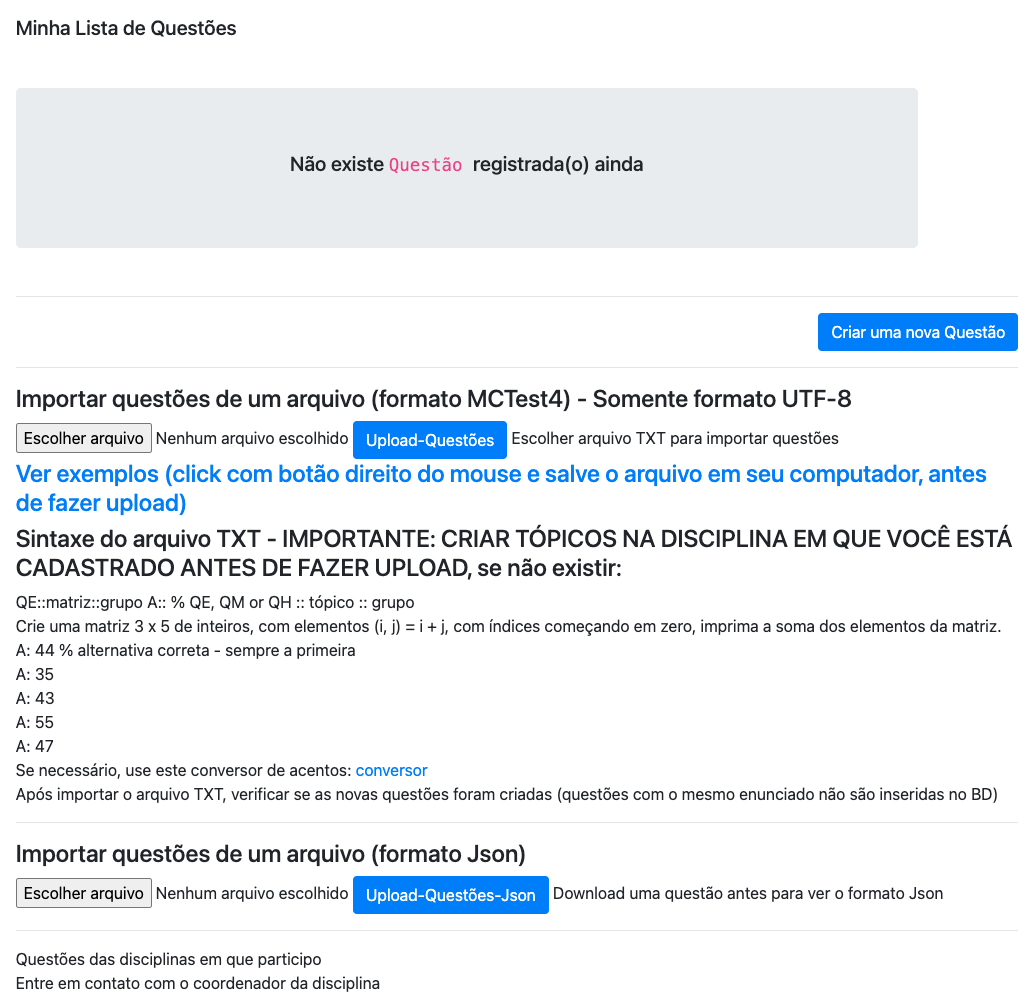
\includegraphics[width=0.9\textwidth]{cap04_figQuestaoMy.png}
  \caption{Tela para o professor visualizar suas questões e criar novas, incluindo importação de formato TXT.}
  \label{fig:cap04_figQuestaoMy}
\end{figure}

\begin{mybox}{pink}{\textbf{Melhorias:\\\vspace{-3mm}\hrule\vspace{3mm}}}
Por enquanto, o botão ``Upload-Questões-Json'' apresentado na Figura \ref{fig:cap04_figQuestaoMy} ainda não está funcionando. Essa funcionalidade será útil para um professor poder fazer \textit{backup} de suas questões e recuperá-las no futuro, caso necessário.
\end{mybox}

Em vez de criar questões por meio da importação de arquivos nos formatos TXT ou JSON, outra opção é criar as questões diretamente no MCTest. Para isso, basta clicar no botão ``Criar uma nova Questão'', apresentado na Figura \ref{fig:cap04_figQuestaoMy}. Em seguida, será aberta a tela apresentada na Figura \ref{fig:cap04_figQuestaoCria}, onde é possível criar uma nova questão. Cada questão deve pertencer a apenas um tópico, e o professor deve escolher um tópico na opção ``Escolher Tópico''. No entanto, um mesmo tópico pode ser compartilhado por mais de uma disciplina, permitindo que as questões sejam utilizadas em diferentes contextos. Em seguida, deve definir uma ``Descrição curta'' e um ``Grupo''. Também deve definir uma ``Descrição'', escolher em ``Tipo'' se é QM ou QT, escolher uma ``Dificuldade'' entre muito fácil (1) e muito difícil (5), definir a ``Taxonomia de Bloom'' e, por fim, informar se a questão é paramétrica ou não. Na Figura \ref{fig:cap04_figQuestaoCria2}, é possível ver um exemplo hipotético de preenchimento dos campos para criar uma nova questão, antes de clicar no botão ``Salvar''.

Vale destacar que ainda serão necessários incluir novos experimentos para avaliar os atributos do formulário da questão. Por exemplo, é importante analisar as características de cada questão utilizando a Teoria de Resposta ao Item (TRI) \cite{2021:Zampirolli.Junior.ea,2021:Zampirolli.Batista.ea}. Adicionalmente, a inclusão da ``Taxonomia de Bloom'' foi motivada pelos artigos de referência de \citeonline{2018:Calsavara.Serra.ea} e \citeonline{2018:Correia.Calsavara.ea}, os quais podem ser consultados na Seção \ref{sec:testeAdaptativo} -- \nameref{sec:testeAdaptativo}.

\begin{figure}[!ht]
  \centering
  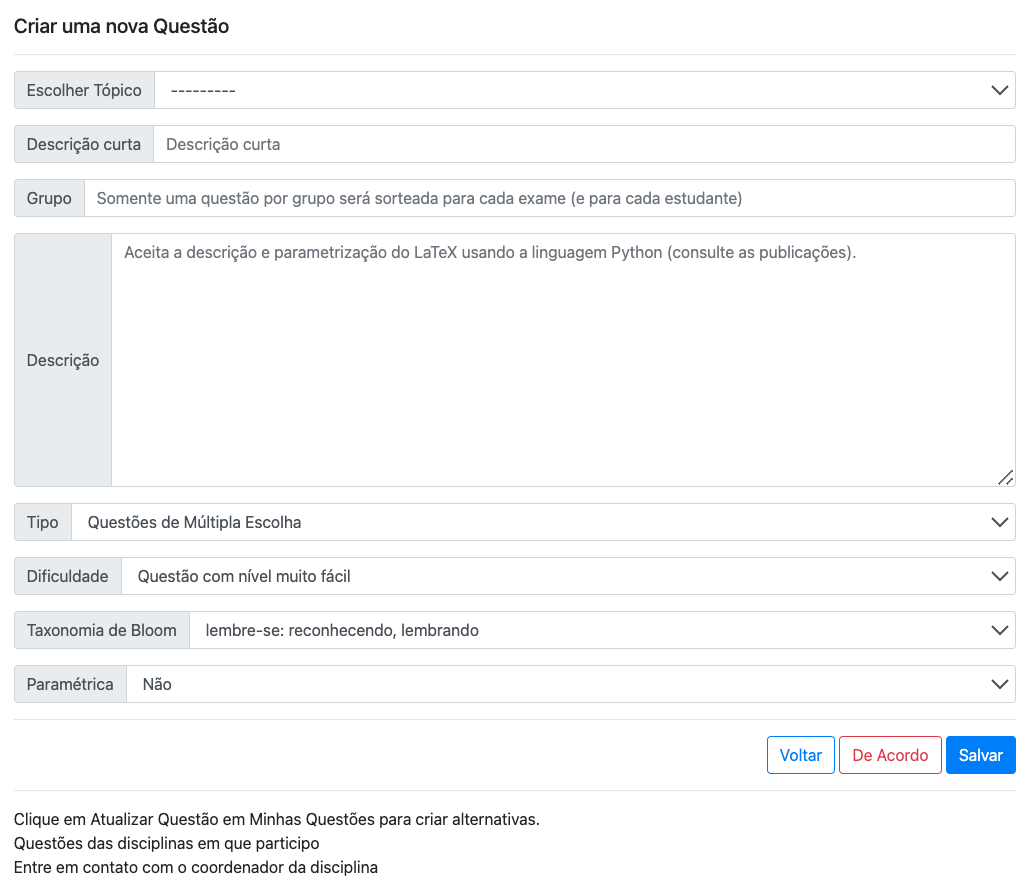
\includegraphics[width=0.9\textwidth]{cap04_figQuestaoCria.png}
  \caption{Tela para um professor criar uma nova questão.}
  \label{fig:cap04_figQuestaoCria}
\end{figure}

\begin{figure}[!ht]
  \centering
  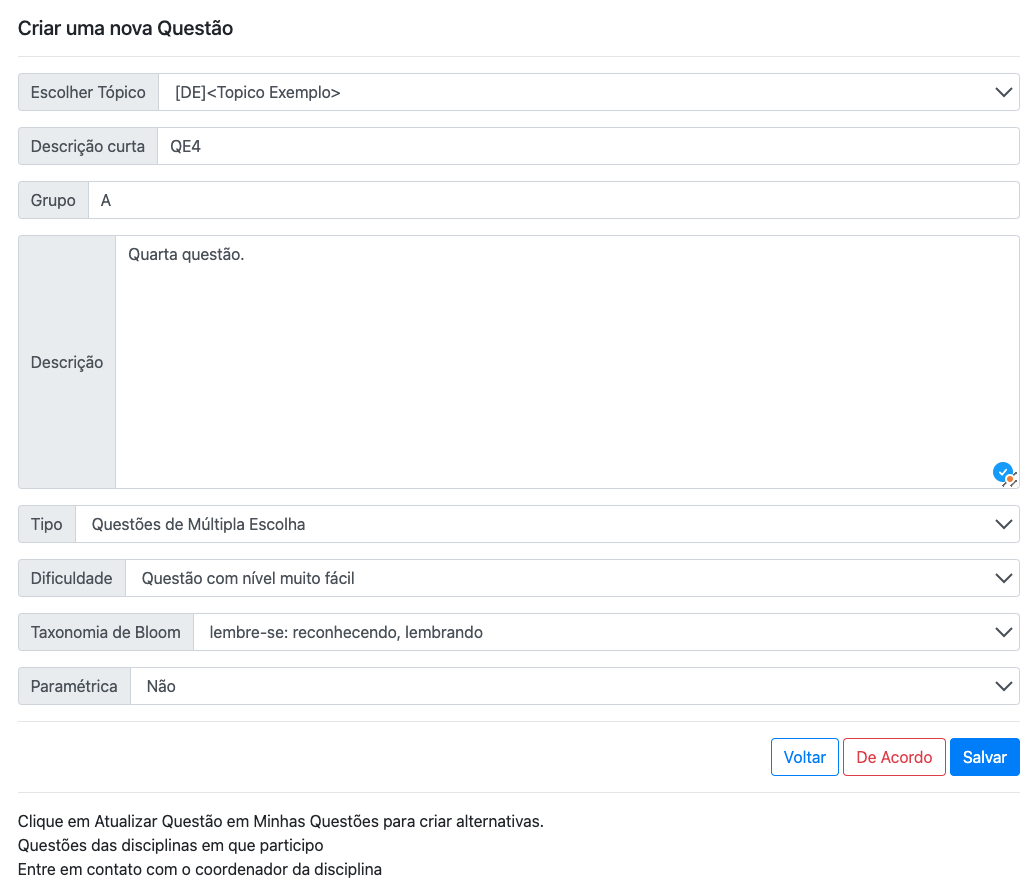
\includegraphics[width=0.9\textwidth]{cap04_figQuestaoCria2.png}
  \caption{Tela com valores preenchidos para criar uma nova questão, antes de clicar no botão ``Salvar''.}
  \label{fig:cap04_figQuestaoCria2}
\end{figure}

\section{Questão de múltipla escolha (QM)}\label{sec:questaoQM}

Nesta seção, serão abordadas as QMs, após a revisão geral das questões apresentadas na seção anterior. A QM é um tipo de questão amplamente utilizado em avaliações educacionais. Ela consiste em apresentar ao estudante uma pergunta ou enunciado, seguido de diversas opções de resposta, variando geralmente de três a cinco alternativas, das quais apenas uma é a correta. O objetivo é verificar se o estudante possui o conhecimento necessário para identificar a resposta correta dentre as opções apresentadas. O MCTest também possibilita a existência de mais de uma alternativa correta, ou a atribuição de pesos diferentes em cada alternativa, mas esses tópicos serão abordados em capítulos futuros.

As QMs são frequentemente utilizadas em testes padronizados, exames de vestibular e concursos públicos, além de serem comuns em avaliações em sala de aula. Elas são consideradas uma forma eficiente e prática de avaliar o conhecimento dos estudantes, já que permitem avaliar inúmeras pessoas em pouco tempo e com baixo custo. No entanto, uma das desvantagens desse tipo de questão é a possibilidade de plágio. O MCTest, porém, consegue minimizar esse problema com a utilização de sorteio das questões e alternativas, gerando exames individuais para cada estudante.

Após a criação da questão, realizada ao clicar no botão ``Salvar'' na Figura \ref{fig:cap04_figQuestaoCria2}, pode ser necessário atualizá-la para adicionar alternativas, caso seja uma QM. Para isso, basta acessar a opção ``Questões'' à direita de ``fzprof'', na Figura \ref{fig:cap04_figQuestao}, e, em seguida, selecionar o botão ``Atualizar'' referente à questão desejada. Será apresentada uma nova tela, conforme ilustrado nas Figuras \ref{fig:cap04_figQuestaoAtualiza} e \ref{fig:cap04_figQuestaoAtualiza2}.

Na Figura \ref{fig:cap04_figQuestaoAtualiza}, o professor pode visualizar a questão em formato PDF clicando no botão ``Criar-PDF'', mostrado na Figura \ref{fig:cap04_figQuestaoAtualizaPDF}. Ao se tratar de uma questão paramétrica que inclui códigos em Python, o professor pode testar a questão separadamente no \href{https://colab.research.google.com/}{Google Colab}, clicando no botão ``Compile-Colab''. O Colab é uma ferramenta muito útil durante a criação de questões paramétricas, já que o MCTest ainda não oferece um ambiente para compilar e depurar códigos. No entanto, esse tópico será abordado em capítulos futuros.

O botão ``Salvar-Json'' salva todas as questões criadas pelo usuário ``fzprof'' em um arquivo no formato JSON. A importação desse arquivo ainda não está disponível no MCTest, como observado anteriormente. 

Complementando a tela de criação de questões, apresentadas nas Figuras \ref{fig:cap04_figQuestaoCria} e \ref{fig:cap04_figQuestaoCria2}, a Figura \ref{fig:cap04_figQuestaoAtualiza} inclui os atributos ``Quem criou'' e a data da ``Última atualização''.  A seguir estão as políticas de edição e uso de questões no MCTest:

\begin{mybox}{corObs}{\textbf{Observações:\\\vspace{-3mm}\hrule\vspace{1mm}}}
\begin{enumerate}
    \item Somente o criador da questão ou o coordenador da disciplina podem editar uma questão;
    \item No entanto, todos os professores cadastrados na disciplina têm permissão para utilizar as questões em seus exames, se concordarem com os termos apresentados na Seção \ref{sec:deAcordo} - \nameref{sec:deAcordo}, disponível na opção ``De Acordo'' da Figura \ref{fig:cap04_figQuestaoAtualiza2}. Essa é uma política adotada na UFABC, mas outras instituições podem adotar políticas diferentes.
\end{enumerate}
\end{mybox}

Além disso, a Figura \ref{fig:cap04_figQuestaoAtualiza} apresenta campos para edição das alternativas da questão. Caso a questão seja dissertativa e possua conteúdo nesses campos, esses valores não serão utilizados ao criar exames.

É importante observar que a tela apresenta apenas uma alternativa, incluindo o ``Texto da Resposta'' e o ``Retorno'' desta alternativa'' (este último é opcional). Para criar novas alternativas, é necessário clicar no botão ``Salvar''. De maneira similar, para excluir uma ou várias alternativas já criadas, basta selecionar a caixa de seleção ``Apagar'' correspondente a cada alternativa que deseja excluir e, em seguida, clicar em ``Salvar''.

\begin{mybox}{corEdicao2}{\textbf{Destaque:\\\vspace{-3mm}\hrule\vspace{3mm}}}
As Figuras \ref{fig:cap04_figQuestaoAtualiza} e \ref{fig:cap04_figQuestaoAtualiza2} foram atualizadas para permitir que o professor efetue o armazenamento no servidor do MCTest de imagens e as inclua em uma questão. O professor pode selecionar um arquivo no formato PNG para importação, sendo necessário tomar precauções quanto ao nome do arquivo, a fim de evitar a sobreposição com outro arquivo de mesmo nome. Uma sugestão consiste em acrescentar um prefixo ao nome do arquivo, tal como \verb|fz_PDI_image01.png|. É importante observar que o nome do arquivo não deve conter caracteres especiais nem espaços em branco. Este arquivo permanecerá no servidor pelo período de 180 dias. Adicionalmente, é relevante ressaltar que a inclusão de imagens em um documento \LaTeX{} pode resultar em considerável lentidão na geração do arquivo PDF. 
\end{mybox}

\begin{mybox}{corEdicao2}{\textbf{Destaque:\\\vspace{-3mm}\hrule\vspace{3mm}}}
A Figura \ref{fig:cap04_figQuestaoAtualiza2} foi atualizada para incluir dois contadores: um para o número de correções realizadas para QM e outro para o número de questões que os estudantes acertaram. Com isso, é possível calcular a acurácia da questão (\textit{corretas/correções}). Além disso, foram adicionados os parâmetros da Teoria de Resposta ao Item (TRI): Discriminação (\(a\)), Habilidade (\(b\)) e Chute (\(c\)). Ver Seção \ref{sec:testeAdaptativo} -- \nameref{sec:testeAdaptativo} para mais detalhes do uso deste recurso.
\end{mybox}

O modelo TRI emprega uma função logística que pode ajustar até três parâmetros associados a um item (questão): a complexidade (ou habilidade), representada pelo modelo logístico de um parâmetro (\(b\), ou 1PLM, conforme mostrado na Curva Característica do Item na Figura \ref{fig:cap04_figTRI}); essa característica é combinada com a capacidade discriminativa (modelo logístico de dois parâmetros \(a\) e \(b\), ou 2PLM); e, por fim, essas características são integradas com a causalidade (acerto pelo chute) (modelo logístico de três parâmetros \(a\), \(b\) e \(c\), ou 3PLM). No estudo \cite{min2021systematic}, os pesquisadores estimam um mínimo de 200, 500 e 1.000 participantes nos modelos 1PLM, 2PLM e 3PLM, respectivamente. A Figura \ref{fig:cap04_figTRI} foi geradada através deste \href{https://colab.research.google.com/drive/1ka7_SR_QB4G7ZPVvH3p_E0bZEbOH1vhK}{Colab}.

\begin{figure}[!ht]
  \centering
  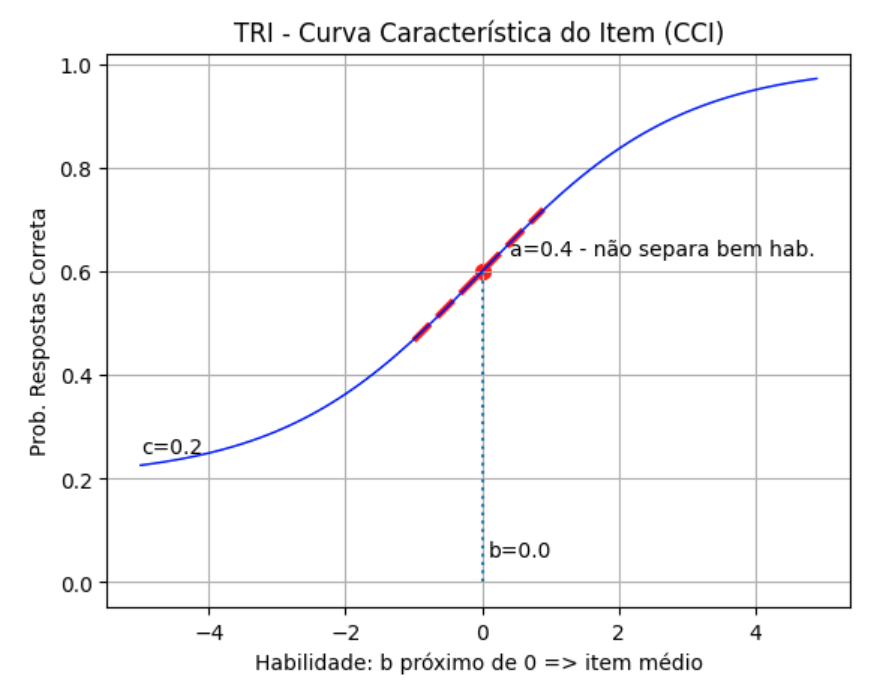
\includegraphics[width=0.9\textwidth]{cap04_figTRI.png}
  \caption{Curva Característica do Item (CCI) de 3-Modelo Logístico de Parâmetros, ou 3PLM. Adaptado de \citeonline{2021:Zampirolli.Batista.ea}.}
  \label{fig:cap04_figTRI}
\end{figure}

\begin{mybox}{corEdicao2}{\textbf{Destaque:\\\vspace{-3mm}\hrule\vspace{3mm}}}
Na Figura \ref{fig:cap04_figQuestaoAtualiza2}, há o botão ``Duplicar esta Questão'' para facilitar o processo de criar uma nova questão com base em uma já existente.
\end{mybox}

\begin{figure}[!ht]
  \centering
  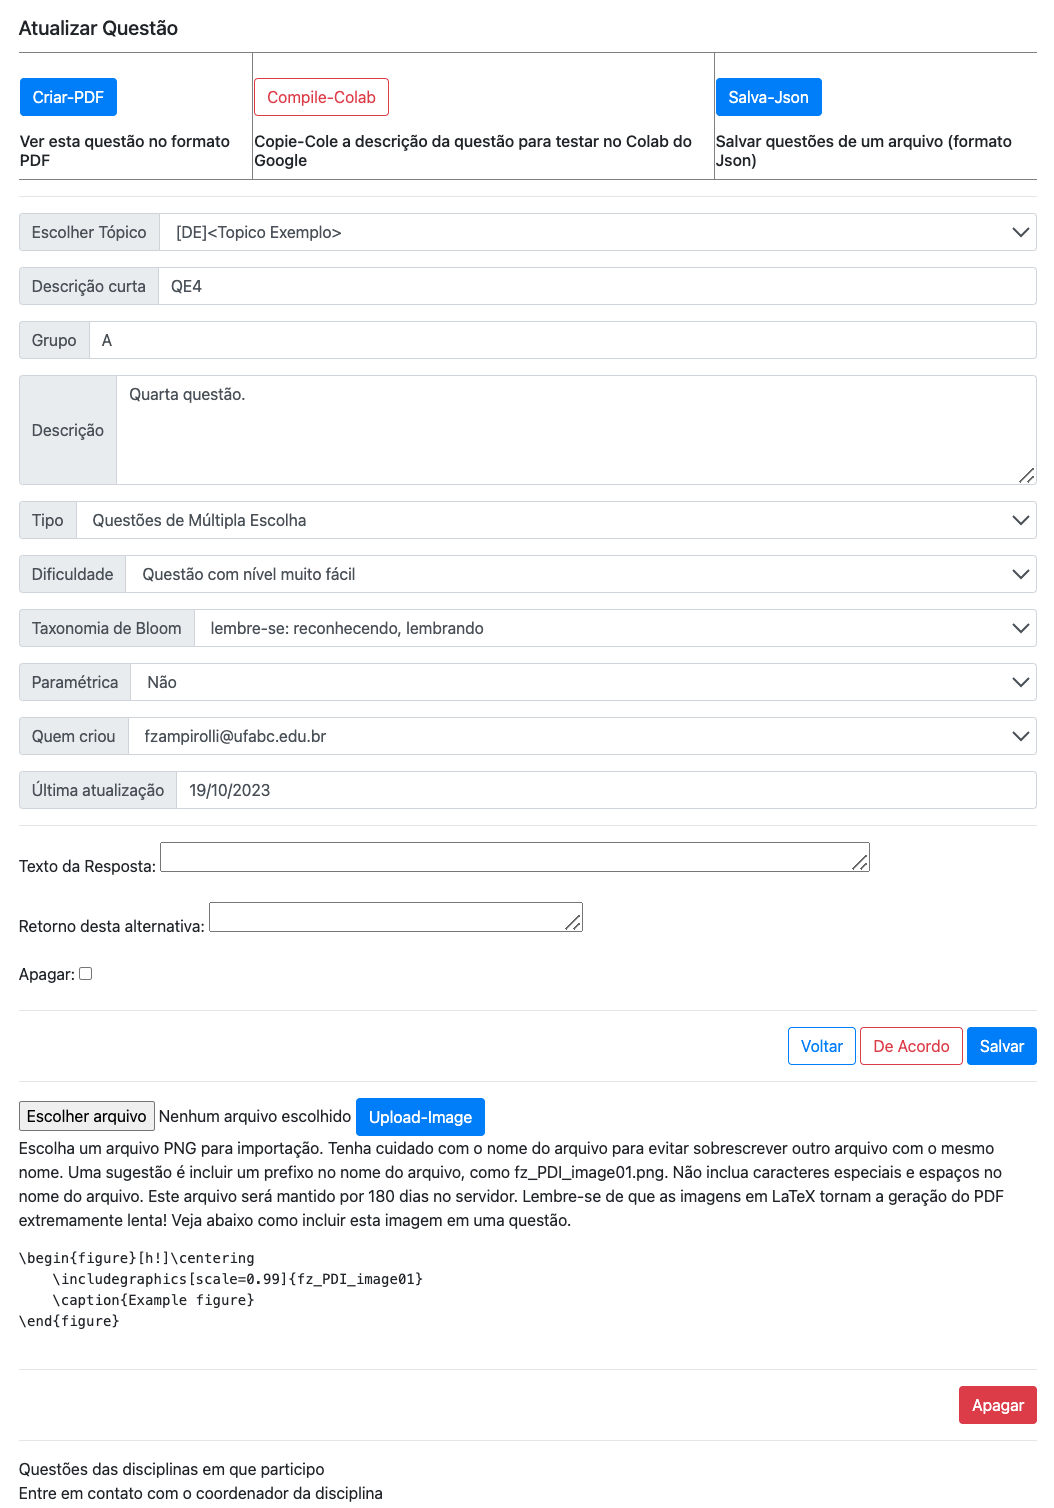
\includegraphics[width=0.9\textwidth]{cap04_figQuestaoAtualiza.png}
  \caption{(Parte 1) Tela de atualização de questão sem alternativas e \textit{feedback}, previamente criada pelo professor.}
  \label{fig:cap04_figQuestaoAtualiza}
\end{figure}

\begin{figure}[!ht]
  \centering
  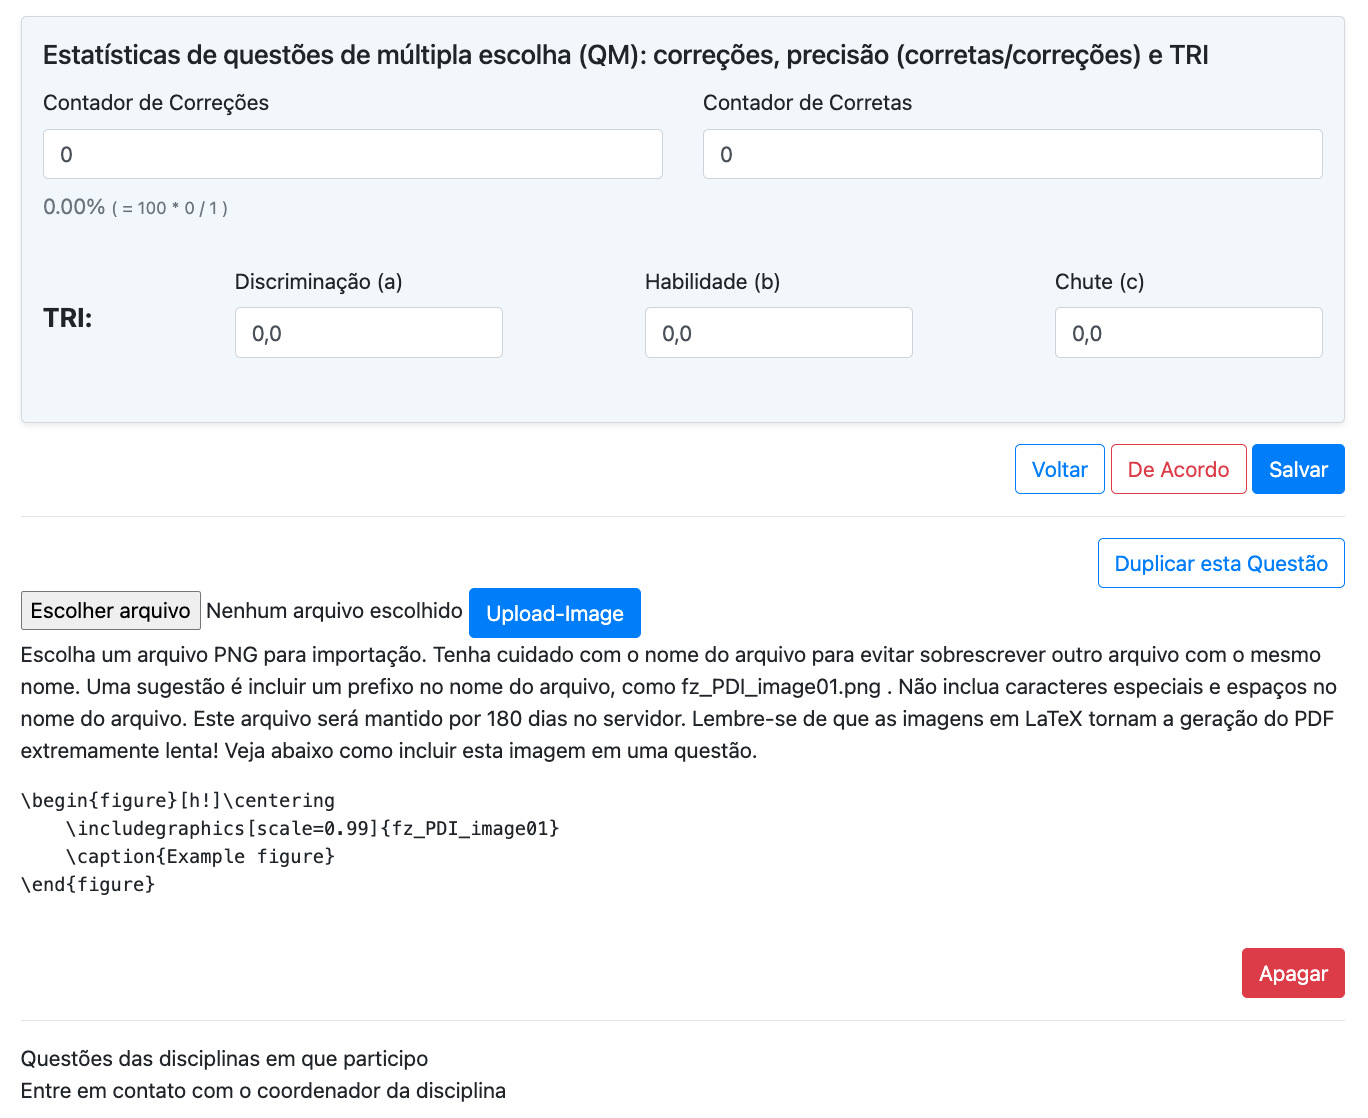
\includegraphics[width=0.9\textwidth]{cap04_figQuestaoAtualiza2.png}
  \caption{(Parte 2) Continuação da tela de atualização de questão, com estatísticas e ajuda para incluir figura.}
  \label{fig:cap04_figQuestaoAtualiza2}
\end{figure}

\begin{figure}[!ht]
  \includegraphics[width=0.35\textwidth]{cap04_figQuestaoAtualizaPDF.png}
  \caption{Recorte do PDF gerado após clicar no botão ``Criar-PDF'', na Figura \ref{fig:cap04_figQuestaoAtualiza}.}
  \label{fig:cap04_figQuestaoAtualizaPDF}
\end{figure}

A Figura \ref{fig:cap04_figQuestaoAtualizaPDF2} apresenta o PDF gerado de uma QM com cinco alternativas preenchidas, após o clique no botão ``Criar-PDF''. O número em verde representa o ID da questão no banco de dados. Os valores em vermelho correspondem às alternativas incorretas, enquanto o valor em azul representa a alternativa correta, considerando a ordem de criação das alternativas definidas na Figura \ref{fig:cap04_figQuestaoAtualiza}.


\begin{figure}[!ht]
  \includegraphics[width=1.0\textwidth]{cap04_figQuestaoAtualizaPDF2.png}
  \caption{Recorte do PDF gerado após clicar no botão ``Criar-PDF'', na Figura \ref{fig:cap04_figQuestaoAtualiza}, para a questão atualizada com cinco alternativas.}
  \label{fig:cap04_figQuestaoAtualizaPDF2}
\end{figure}


\section{Questão dissertativa (QT)}\label{sec:introducaoTextoQT}

Para criar uma questão dissertativa (QT -- de texto), basta selecionar a opção ``Questão Dissertativa'' no campo Tipo, conforme apresentado na Figura \ref{fig:cap04_figQuestaoCria}. É importante observar que o processo de criação para QTs é similar ao processo para QMs, apresentado na seção anterior.

A Figura \ref{fig:cap04_figQuestaoAtualizaPDF3} apresenta um exemplo de PDF gerado para uma QT. Nesse tipo de questão, o estudante deve escrever uma resposta livremente, sem a necessidade de escolher entre alternativas predefinidas. As cinco linhas que aparecem nessa questão são impressas utilizando o comando pré-definido \verb|\drawLines{5}|. É comum que as QTs sejam usadas para avaliar a compreensão do estudante sobre um determinado tema, suas habilidades de análise e argumentação, ou ainda para avaliar a sua capacidade de escrever de forma clara e organizada.

\begin{figure}[!ht]
  \includegraphics[width=1\textwidth]{cap04_figQuestaoAtualizaPDF3.png}
  \caption{Recorte do PDF gerado após clicar no botão ``Criar-PDF'', na Figura \ref{fig:cap04_figQuestaoAtualiza}, para uma questão dissertativa (``Type: QT'').}
  \label{fig:cap04_figQuestaoAtualizaPDF3}
\end{figure}

Na Figura \ref{fig:cap04_figQuestaoAtualizaTesteMesa}, apresenta-se a alteração do campo ``Descrição'' da Figura \ref{fig:cap04_figQuestaoAtualiza}, utilizando a sintaxe do \LaTeX, uma linguagem de marcação amplamente utilizada na produção de documentos acadêmicos. O PDF gerado desta questão é apresentado na Figura \ref{fig:cap04_figQuestaoAtualizaPDF4}

\begin{figure}[!ht]
  \includegraphics[width=1.0\textwidth]{cap04_figQuestaoAtualizaTesteMesa.png}
  \caption{Recorte da ``Descrição'' de uma QT de teste de mesa.}
  \label{fig:cap04_figQuestaoAtualizaTesteMesa}
\end{figure}

A questão avaliará as competências e habilidades dos estudantes em relação aos conceitos de condicional e repetição na programação. Esses conceitos são fundamentais para o desenvolvimento de algoritmos e programas computacionais, e são frequentemente abordados em disciplinas introdutórias de programação.


\begin{figure}[!ht]
  \includegraphics[width=1.0\textwidth]{cap04_figQuestaoAtualizaPDF4.png}
  \caption{Recorte do PDF gerado da QT de teste de mesa.}
  \label{fig:cap04_figQuestaoAtualizaPDF4}
\end{figure}

\section{Considerações finais}

O MCTest é uma plataforma completa que oferece diversas funcionalidades para a criação de exames. Desde QMs e QTs até questões paramétricas que envolvem códigos em Python. O MCTest oferece recursos para os professores poderem criar avaliações personalizadas para suas turmas. Além disso, a plataforma permite que as questões sejam organizadas em bancos de dados para facilitar a criação de exames.

No entanto, é importante destacar que o MCTest é apenas uma ferramenta auxiliar no processo de avaliação. A qualidade da avaliação depende não apenas das questões criadas, mas também da forma como são elaboradas e aplicadas. É fundamental que os professores sejam cuidadosos na escolha das questões e na definição do nível de dificuldade adequado para cada turma. A utilização do MCTest deve ser sempre acompanhada de uma análise crítica e cuidadosa sobre a adequação das questões e a efetividade do processo de avaliação.

Por fim, espera-se que este documento tenha sido útil para os professores interessados em utilizar o MCTest em suas disciplinas. No próximo capítulo, serão abordadas questões paramétricas que envolvem códigos em Python. \cleardoublepage
%%%%%%%%%%%%%%%%%%%%%%%%%%%%%%%%%%%%%%%%%%%%%%%%%%%%%%%
\mychapter{Questões paramétricas}\label{ch:questoesCodigoMCTest}

No capítulo anterior, foi apresentada a criação de questões estáticas de múltipla escolha (QMs) e dissertativas (QTs), incluindo uma questão típica utilizada em disciplinas de lógica de programação na UFABC, apresentada na Figura \ref{fig:cap04_figQuestaoAtualizaPDF4}. É possível criar essas questões utilizando \LaTeX, uma linguagem de preparação de documentos de alta qualidade e profissionalismo, com recursos avançados para controle de tipos de letra, espaçamento, numeração de seções, referências bibliográficas e equações matemáticas, entre outros. \LaTeX{} é gratuita e está disponível para vários sistemas operacionais.

A linguagem \LaTeX{} foi criada no início da década de 1980 pelo matemático e cientista da computação Leslie Lamport \cite{lamport1985latex}. Ela é baseada no \TeX, uma linguagem de marcação desenvolvida por Donald Knuth na década de 1970 para produzir documentos com alta qualidade tipográfica para sua série de livros ``\textit{The Art of Computer Programming}''. O \TeX{} se tornou popular para a produção de documentos científicos, técnicos e matemáticos e ainda é amplamente utilizado atualmente.

Para contornar a sintaxe complexa e de difícil programação do \LaTeX{}, no MCTest foi introduzida a possibilidade de intercalar trechos em \LaTeX{} com trechos de código em Python. Python é uma linguagem de programação de alto nível, interpretada e de propósito geral, criada no início da década de 1990 por Guido van Rossum, e atualmente é uma das linguagens de programação mais populares do mundo~\footnote{Levantamento das linguagens de programação mais populares em 2023: \href{https://survey.stackoverflow.co/2023}{survey.stackoverflow.co/2023} e  \href{https://pypl.github.io/PYPL.html}{pypl.github.io/PYPL.html}.}. Com uma ampla variedade de aplicações em áreas como desenvolvimento web, ciência de dados, inteligência artificial e automação de processos, Python é conhecida por sua sintaxe clara e legível, facilitando a escrita e a leitura de código. 

O MCTest proporciona aos usuários a capacidade de criar questões diversas e paramétricas, combinando o uso do formato \LaTeX{} e da linguagem de programação Python. Essa funcionalidade será apresentada neste capítulo. Em capítulos futuros, na Parte - \ref{part:experimentos} - \textbf{Experimentos}, serão exploradas com mais detalhes essa característica fundamental do MCTest de criar questões paramétricas.
%
Essa abordagem proporciona maior flexibilidade na criação de questões personalizadas e permite uma fácil manipulação dos parâmetros definidos pelos professores. Dessa forma, a criação de questões torna-se mais eficiente e adaptável às necessidades específicas de cada disciplina.

Apesar dessa possibilidade, muitas vezes a criação de questões paramétricas ainda exige habilidades de programação por parte do professor. No entanto, quando há um grupo de professores interessados e uma grande demanda de avaliações para milhares de estudantes, o MCTest oferece a gestão de avaliações utilizando um banco de questões que podem ser facilmente reaproveitadas em avaliações futuras. Essa abordagem já foi avaliada em várias publicações científicas, demonstrando eficiência e eficácia em avaliações, como apresentado em \href{http://vision.ufabc.edu.br}{vision.ufabc.edu.br}. 

\section{QM paramétrica}

A criação de QMs é uma tarefa comum para professores de diversas áreas do conhecimento. Para tornar esse processo mais eficiente, é possível utilizar recursos de programação. Nesta seção, será abordada a QM paramétrica, que permite criar questões com variações de parâmetros. Isso possibilita a criação de inúmeras questões com facilidade e rapidez. Serão apresentados exemplos de como criar questões paramétricas em Python, utilizando o MCTest como plataforma. Serão abordadas diferentes técnicas de parametrização, permitindo ao professor escolher a que melhor se adapta à sua habilidade em programação.


\subsection{Um exemplo}

Suponha que você seja um professor de matemática e deseje criar várias QMs sobre a fórmula da área do círculo. Embora este exemplo seja bastante simples, é possível generalizar para questões mais complexas. Para alcançar esse objetivo, você pode utilizar o método em Python apresentado no Código \ref{lst:codigoAreaCirculo}.


\begin{listing}[!ht]
\begin{myboxCode}{corCodigo}{\textbf{Código: } método \verb|area_circulo(raio)|}\vspace{3mm}
\hrule
\begin{minted}[xleftmargin=20pt,linenos=true]{python}
import math

def area_circulo(raio):
  return math.pi * raio ** 2
\end{minted}
\end{myboxCode}
\caption{Exemplo de método para calcular a área de um círculo.}
\label{lst:codigoAreaCirculo}
\end{listing}


Com base no método apresentado no Código \ref{lst:codigoAreaCirculo}, é possível gerar diversas QMs sobre a área do círculo, com as seguintes variações:

\begin{enumerate}
\item A questão deve ter 4 alternativas de resposta;
\item O raio do círculo deve variar aleatoriamente;
\item A alternativa correta deve ser calculada com base no valor do raio;
\item As demais alternativas erradas devem ter valores distintos.
\end{enumerate}

A seguir, serão apresentados três exemplos de questões para calcular a área do círculo, com raios escolhidos aleatoriamente:

\begin{description}
    
    \item \textbf{1) Qual é a área do círculo de raio 2?}

\begin{multicols}{4}
\begin{enumerate}[label=\Alph*.]
\item 3,14
\item 6,28
\item 12,56
\item 25,12
\end{enumerate}
\end{multicols}

    \item \textbf{2) Qual é a área do círculo de raio 4?}

\begin{multicols}{4}
\begin{enumerate}[label=\Alph*.]
\itemsep0pt\parskip0pt\parsep0pt
\item 12,56
\item 25,12
\item 37,68
\item 50,24
\end{enumerate}\normalsize
\end{multicols}

    \item \textbf{3) Qual é a área do círculo de raio 3?}

\begin{multicols}{4}
\begin{enumerate}[label=\Alph*.]
\itemsep0pt\parskip0pt\parsep0pt
\item 9,42
\item 12,56
\item 15,70
\item 18,84
\end{enumerate}\normalsize
\end{multicols}

\end{description}


Nos exemplos ilustrativos apresentados, o método \verb|area_circulo| pode ser utilizado para calcular a resposta correta para cada alternativa de resposta. A variação aleatória do raio pode ser realizada com a ajuda da biblioteca \verb|random| do Python. Por fim, as alternativas erradas podem ser calculadas, também utilizando o método \verb|area_circulo|, com base no valor do raio, garantindo a não repetição de alternativas. A seguir, será apresentado esse exemplo implementado no MCTest.

\subsection{QM paramétrica no MCTest}\label{sec:QMparametrica}

É possível parametrizar QMs no MCTest de várias maneiras, dependendo das habilidades de programação em Python do professor. Algumas dessas maneiras são apresentadas nesta seção.

\begin{mybox}{corObs}{\textbf{Observações:\\\vspace{-3mm}\hrule\vspace{1mm}}}
\begin{enumerate}
    \item A descrição da questão no MCTest (campo ``Descrição'' na Figura \ref{fig:cap04_figQuestaoAtualiza}), que pode incluir textos em \LaTeX{} integrados com códigos em Python, é a parte mais importante na criação de questões paramétricas. A partir deste capítulo, não será mais apresentada uma captura de tela da questão, como foram realizados nos dois capítulos anteriores. Para criar uma QM ou QT paramétrica basta alterar o parâmetro ``Paramétrica'' de ``Não'' para ``Sim'', nas telas de criação ou alteração de questão;
    \item A parte mais complicada na criação de questões paramétricas no MCTest é lidar com possíveis erros que podem ser retornados pelo MCTest ao tentar criar o PDF. Para tentar resolver esse problema, foi criado um \textit{notebook} no Google Colab, acessado ao clicar no botão ``Compile-Colab'' nas telas de alteração de questão, como apresentado na Figura \ref{fig:cap04_figQuestaoAtualiza}.
\end{enumerate}
\end{mybox}

\subsubsection{Exemplo 1}

Veja uma descrição da questão paramétrica para calcular a área de um círculo, implementada no MCTest, no Código \ref{lst:questaoQM_AreaCirculoEx1}. Todo o texto que aparece até a linha 6, contendo \verb|[[def:|, fará parte do enunciado da questão e pode utilizar a sintaxe do \LaTeX. As partes paramétricas deste enunciado ocorrem nas instruções em Python entre as marcações \verb|[[code:| e \verb|]]|. Geralmente, essas instruções são variáveis definidas em Python entre as marcações \verb|[[def:| e \verb|]]|, neste exemplo, entre as linhas 6 e 30.

\begin{mybox}{corCopia}{\textbf{Marcações principais definidas no MCTest:\\\vspace{-3mm}\hrule\vspace{1mm}}}
\begin{enumerate}
    \item Instruções que podem representar a parte paramétrica do enunciado da questão ou das alternativas são colocadas entre as marcações \verb|[[code:| e \verb|]]|, conforme exemplificado na linha 1 do Código \ref{lst:questaoQM_AreaCirculoEx1};
    \item Após esse enunciado, um único bloco de código em Python deve ser definido entre as marcações \verb|[[def:| e \verb|]]|, como ilustrado entre as linhas 6 e 30 do exemplo. Todo o texto após esse bloco é descartado do enunciado da questão.
\end{enumerate}
\end{mybox}

\begin{mybox}{corEdicao2}{\textbf{Destaque:\\\vspace{-3mm}\hrule\vspace{3mm}}}
Em alguns casos, ocorre um erro no retorno da expressão regular para capturar as variáveis ou instruções delimitadas por \verb|[[code:| e \verb|]]|. Nesses casos, é necessário adicionar um espaço antes de \verb|[[code:| e após \verb|]]|. O método \verb|get_code| disponível no GitHub em \href{https://github.com/fzampirolli/mctest/blob/master/topic/UtilsMCTest4.py}{UtilsMCTest4.py} propõe uma sugestão de modificação na expressão regular. No entanto, essa sugestão apresenta uma falha quando ocorre uma sequência de \verb|]]| dentro de \verb|[[def:| e \verb|]]|. Assim, para evitar problemas, use sempre espaços antes de \verb|[[code:| e após \verb|]]|.
\end{mybox}

Se as marcações de início e fim de bloco ou instruções aparecerem erroneamente, ou se houver algum erro no código Python, mensagens de erro do compilador Python poderão ser exibidas, mas sem fornecer muitos detalhes sobre o erro específico. Portanto, é fundamental testar o código Python fora do MCTest, por exemplo, utilizando o \textit{notebook} do Google Colab. Para acessar o \textit{notebook}, basta clicar no botão ``Compile-Colab'' nas telas de alteração de questão, como mostrado na Figura \ref{fig:cap04_figQuestaoAtualiza}. Experimente adicionar espaços inesperados, como \verb|[[code: raio1]]| ou \verb|[ [code:raio1]]|, salve e clique em ``Cria-PDF''. Isso permitirá identificar erros e depurar a questão no MCTest, seguindo os seguintes exemplos:

\begin{myboxCode}{corObs}{\textbf{Alguns exemplos de erros comuns que podem ocorrer:\\\vspace{-3mm}\hrule\vspace{3mm}}}
Experimente incluir esses erros, salve e crie o PDF para identificar e corrigir possíveis problemas futuros:
\begin{enumerate}
    \item \verb|[[code: raio1]]| -- espaço não esperado -- retorna:\\ 
    \verb|ERROR in [[code: ... ]]: unmatched ’]’ (<string>, line 1) raio1]]?|
    
    \item \verb|[[code:Raio1]]| -- ``R'' maiúsculo -- retorna:\\
    \verb|ERROR in [[code: ... ]]: name ’Raio1’ is not defined Raio1|
    
    \item Bloco de código no método \verb|area_circulo| sem \textit{identação} correta -- retorna:\\
    \verb|ERROR in [[def: ... ]]: unexpected indent (<string>, line 7)|
    
    \item Sem a linha \verb|import math| no método \verb|area_circulo| -- retorna:\\
    \verb|ERROR in [[def: ... ]]: name ’math’ is not defined|
    
    \item Sem os ``:'' no final da linha do método  \verb|area_circulo| -- retorna:\\
    \verb|ERROR in [[def: ... ]]: invalid syntax (<string>, line 5)|
    
    \item \verb|[ [def:| ou  \verb|[[def :|  -- espaço não esperado -- retorna:\\
    \verb|ERROR in [[code: ... ]]: name ’raio1’ is not defined raio1| 
    
\end{enumerate}
\end{myboxCode}

Observe que, nesse sexto caso, o erro retornado é que a variável \verb|raio1| não foi definida. Isso ocorreu porque o MCTest não encontrou o bloco de código Python entre as marcações \verb|[[def:| e \verb|]]|. Certifique-se de ter incluído corretamente o bloco de código necessário para definir a variável \verb|raio1| e verifique se não há erros de digitação ou formatação nas marcações. Essa etapa é crucial para garantir o funcionamento correto da questão paramétrica no MCTest.

\begin{listing}[!ht]
\begin{myboxCode}{corCodigo}{\textbf{Questão: }}\vspace{3mm}
\hrule
\begin{minted}[xleftmargin=20pt,linenos=true]{python}
Qual é a área do círculo de raio [[code:raio1]]?

% comentário em LaTeX. Observe que a variável raio1, após "code:" 
% foi definida na linha 15 abaixo

[[def: # comentário em Python
# o bloco de código Python deve sempre iniciar com a linha anterior!
import random

def area_circulo(raio): # método para calcular a área do círculo
    import math # necessário importar biblioteca(s) no método
    return math.pi * raio ** 2

# lista de 4 raios aleatórios entre 20 e 50
raio1,raio2,raio3,raio4 = random.sample(range(20,51), 4)

# formata as áreas com 2 casas decimais
area1 = f"{area_circulo(raio1):.2f}"
area2 = f"{area_circulo(raio2):.2f}"
area3 = f"{area_circulo(raio3):.2f}"
area4 = f"{area_circulo(raio4):.2f}"

# incluir nas alternativas:
# [[code:area1]]
# [[code:area2]]
# [[code:area3]]
# [[code:area4]]

# o bloco de código Python deve sempre terminar com a próxima linha
]]
Todo o texto que aparece após a linha anterior é ignorado.
\end{minted}
\end{myboxCode}
\caption{Exemplo de QM paramétrica para calcular a área do círculo.}
\label{lst:questaoQM_AreaCirculoEx1}
\end{listing}


\subsubsection{Exemplo 2}\label{sec:QMparametricaEx2}

Quando as alternativas de uma QM paramétrica assumem apenas valores inteiros, é possível utilizar o método \verb|createWrongAnswers| desenvolvido e disponibilizado no MCTest. No entanto, algumas exigências são necessárias, como apresentado no Código \ref{lst:questaoQM_AreaCirculoEx2}. 

Primeiramente, é necessário criar uma variável global chamada \verb|correctAnswer|, conforme mostrado na linha 12 do código. Em seguida, atribui-se a resposta correta a essa variável, como ilustrado na linha 14. 

No que diz respeito às alternativas da questão, é importante incluir na primeira alternativa o conteúdo da linha 17, sem o comentário. Na segunda alternativa, deve-se utilizar o conteúdo da linha 18, também sem o comentário. Na linha 18, o método irá gerar três valores aleatórios distintos entre \verb|correctAnswer|$-10$ e \verb|correctAnswer|$+10$. 

É importante observar que, nesse caso, as questões geradas não são consideradas ``ótimas'', pois os estudantes podem deduzir que a resposta correta não está nos extremos dos valores fornecidos, conforme ilustrado na Figura \ref{fig:cap05_questaoQM_AreaCirculoPDF}. 
Em QMs, o texto em verde (\verb|#2450|) representa a identificação da questão no banco de dados. Azul (\verb|#0|) representa a primeira alternativa na tela de criação ou alteração da questão. As demais alternativas em vermelho (\verb|*1|, \verb|*2| e \verb|*3|) são as três alternativas erradas criadas pelo método \verb|createWrongAnswers|.


\begin{listing}[!ht]
\begin{myboxCode}{corCodigo}{\textbf{Questão: }}\vspace{3mm}
\hrule
\begin{minted}[xleftmargin=20pt,linenos=true]{python}
Qual é a área do círculo de raio [[code:raio1]]?

[[def:
import random

def area_circulo(raio): 
    import math # necessário importar biblioteca(s) no método
    return math.pi * raio ** 2

raio1 = random.randint(10, 51) # sorteia valor entre 10 e 50

global correctAnswer # variável necessária para usar o método 
# createWrongAnswers, a resposta deve ter valor inteiro
correctAnswer = int(area_circulo(raio1)) 

# incluir nas alternativas da questão: 
# [[code:correctAnswer]] % primeira alternativa (sempre) correta
# [[code:createWrongAnswers([3,10])]] % cria 3 alter. erradas +/- 10
]]
\end{minted}
\end{myboxCode}
\caption{Exemplo de QM paramétrica para calcular a área do círculo, utilizando o método \texttt{createWrongAnswers}.}
\label{lst:questaoQM_AreaCirculoEx2}
\end{listing}

\begin{figure}[!ht]
  \includegraphics[width=0.5\textwidth]{cap05_questaoQM_AreaCirculoPDF.png}
  \caption{Recorte do PDF gerado para a questão definida no Código \ref{lst:questaoQM_AreaCirculoEx2}.}
  \label{fig:cap05_questaoQM_AreaCirculoPDF}
\end{figure}


\section{QT paramétrica}

Os conceitos apresentados anteriormente para as QMs paramétricas são aplicáveis também às QTs paramétricas, com a distinção de que não há necessidade de considerar as alternativas da questão. Em vez disso, é possível definir uma única resposta correta, se necessário. Nesta seção, serão fornecidos três exemplos adicionais da questão de teste de mesa introduzida no capítulo anterior (Seção \ref{sec:introducaoTextoQT} -- \nameref{sec:introducaoTextoQT}), agora sob a perspectiva paramétrica.

No primeiro exemplo, foi criada uma questão com três parâmetros aleatórios. No segundo exemplo, foi adicionado um gabarito para esses parâmetros aleatórios, implementando a solução do pseudocódigo apresentado em Python e adicionando comandos \verb|print| em locais estratégicos para imprimir a tabela com o gabarito. Por fim, no último exemplo, foi utilizado um recurso avançado de rastreamento de instruções, métodos e exceções.
%
Esses exemplos mostram o poder da parametrização no MCTest para criar questões personalizadas e detalhadas.

\subsection{Exemplo 1 -- Teste de mesa}

Nesta seção, será abordada a parametrização da questão de teste de mesa ilustrada na Figura \ref{fig:cap05_questaoQT_TesteMesaEx1PDF} e apresentada no Código \ref{lst:questaoQT_TesteMesaEx1}, para exemplificar o processo. As partes paramétricas estão localizadas nas linhas 4, 7, 8 e 9 na questão, com os parâmetros \verb|N1|, \verb|N2| e \verb|N3|, cujos valores são definidos aleatoriamente no bloco de código Python nas linhas 38, 39 e 40, respectivamente. O PDF correspondente a essa questão é apresentado na Figura \ref{fig:cap05_questaoQT_TesteMesaEx1PDF}.


\begin{listing}[!ht]
\begin{myboxCode}{corCodigo}{\textbf{Questão: }}\vspace{3mm}
\hrule
\begin{minted}[xleftmargin=20pt,linenos=true]{python}
Preencha a tabela com os valores corretos das variáveis contador e soma 
em cada iteração do laço.  Além disso, considere os números das linhas do 
código para preencher a tabela, a fim de facilitar a referência. Considere 
inicialmente maximo=[[code:N1]], contador=[[code:N2]] e soma=[[code:N3]].

\begin{verbatim}
1. Inicializar a variável maximo com [[code:N1]]
2. Inicializar a variável contador com [[code:N2]]
3. Inicializar a variável soma com [[code:N3]]
4. Enquanto contador <= maximo faça
5.     Se contador é par então
6.         soma = soma + contador
7.     Senão
8.         soma = soma - contador
9.     Fim se
10.    Incrementar contador em 1
11. Fim enquanto
12. Imprimir o valor da variável soma
\end{verbatim}

\begin{tabular}{|c|c|c|c|}
\hline
\textbf{linha} & \textbf{maximo} & \textbf{contador} & \textbf{soma} \\
\hline
& & & \\ \hline
& & & \\ \hline
&  & & \\ \hline
&  & & \\ \hline
&  & & \\ \hline
&  & & \\ \hline
&  & & \\ \hline
&  & & \\ \hline
&  & & \\ \hline
\end{tabular}

[[def:
import random
N1 = random.randint(7,16)
N2 = random.randint(1,6)
N3 = random.randint(1,5)
]]
\end{minted}
\end{myboxCode}
\caption{Exemplo simples de descrição de QT paramétrica para teste de mesa.}
\label{lst:questaoQT_TesteMesaEx1}
\end{listing}

\begin{figure}[!ht]
  \includegraphics[width=0.9\textwidth]{cap05_questaoQT_TesteMesaEx1PDF.png}
  \caption{Recorte do PDF gerado para a questão definida no Código \ref{lst:questaoQT_TesteMesaEx1}.}
  \label{fig:cap05_questaoQT_TesteMesaEx1PDF}
\end{figure}

\subsection{Exemplo 2 -- Teste de mesa e gabarito}

É possível aprimorar o exemplo anterior expandindo-o para gerar o gabarito correspondente a cada valor aleatório gerado para as variáveis \verb|N1|, \verb|N2| e \verb|N3|. Para essa finalidade, foi criado um método em Python que implementa o algoritmo da questão. Devido à quantidade de linhas na descrição dessa questão, os códigos correspondentes foram divididos e estão disponíveis nos fragmentos dos Códigos \ref{lst:questaoQT_TesteMesaEx2Parte1} e  \ref{lst:questaoQT_TesteMesaEx2Parte2}.

Nesta nova versão, o gabarito foi adicionado ao PDF utilizando as linhas 37 a 41 do Código \ref{lst:questaoQT_TesteMesaEx2Parte1}. Na linha 37, azul e o tamanho \verb|small| foram definidos para a variável \verb|tabela|, conforme mostrado na Figura \ref{fig:cap05_questaoQT_TesteMesaEx2PDF}. Caso o professor não deseje exibir esse gabarito na folha de atividade, basta utilizar a cor \verb|white|. Na linha 39, a variável \verb|tabela|, sendo uma \textit{string}, é definida na segunda parte do código, no Código \ref{lst:questaoQT_TesteMesaEx2Parte2}.

Nesta versão, foi criado o método \verb|gerar_gabarito| para retornar a tabela atualizada para incluir as linhas específicas do algoritmo com os espaços correspondentes para preencher com os valores corretos das variáveis \verb|maximo|, \verb|contador| e \verb|soma|. 

O trecho entre as linhas 30 e 34 do Código \ref{lst:questaoQT_TesteMesaEx2Parte2} apresenta um exemplo de uso do código, no qual são gerados valores aleatórios para \verb|N1|, \verb|N2| e \verb|N3| até que a tabela gerada tenha entre 10 e 15 linhas (exclusivamente). Esse trecho será analisado linha por linha:

\begin{description}
    \item \verb|while True|: isso cria um \textit{loop} infinito que será executado até que a condição na linha 33 seja satisfeita e o \textit{loop} seja interrompido na linha 34;
    \item \verb|N1, N2, N3 = random.sample(range(4, 20), 3)|: aqui é usado o método \verb|sample| da biblioteca \verb|random| para gerar três valores aleatórios, sem repetição, no intervalo de 4 a 19. Esses valores são atribuídos às variáveis \verb|N1|, \verb|N2| e \verb|N3|;
    \item \verb|tabela = gerar_gabarito(N1, N2, N3)|: o método é chamado \verb|gerar_gabarito| passando os valores aleatórios \verb|N1|, \verb|N2| e \verb|N3| como argumentos. Esse método retorna a tabela formatada com os valores corretos das variáveis \verb|maximo|, \verb|contador| e \verb|soma|;
    \item \verb|if 10 < len(tabela.split('\n')) < 15: break|: aqui é verificado o número de linhas na tabela gerada. Se o número de linhas estiver entre 10 e 15 (exclusivamente), a condição é satisfeita e o \textit{loop} é interrompido com o uso do comando \textit{break}.
\end{description}

Dessa forma, esse trecho de código permite gerar valores aleatórios para as variáveis \verb|N1|, \verb|N2| e \verb|N3| repetidamente até que a tabela gerada tenha o número de linhas desejado. Isso garante que todas as variações tenham dificuldades de resolução semelhantes, testando diferentes casos. Neste exemplo simples, é possível gerar $15*14*13$ variações (pois os valores sortados não se repetem usando o comando \verb|random.sample(range(4, 20), 3)|), mas apenas aquelas que resultarem em tabelas com 11 a 14 linhas serão consideradas.

\begin{listing}[!ht]
\begin{myboxCode}{corCodigo}{\textbf{Questão: }}\vspace{3mm}
\hrule
\begin{minted}[xleftmargin=20pt,linenos=true]{python}
Preencha a tabela com os valores corretos das variáveis contador e soma 
em cada iteração do laço.  Além disso, considere os números das linhas do 
código para preencher a tabela, a fim de facilitar a referência. Considere 
inicialmente maximo=[[code:N1]], contador=[[code:N2]] e soma=[[code:N3]].

\begin{verbatim}
1. Inicializar a variável maximo com [[code:N1]]
2. Inicializar a variável contador com [[code:N2]]
3. Inicializar a variável soma com [[code:N3]]
4. Enquanto contador <= maximo faça
5.     Se contador é par então
6.         soma = soma + contador
7.     Senão
8.         soma = soma - contador
9.     Fim se
10.    Incrementar contador em 1
11. Fim enquanto
12. Imprimir o valor da variável soma
\end{verbatim}


\begin{tabular}{|c|c|c|c|}
\hline
\textbf{linha} & \textbf{maximo} & \textbf{contador} & \textbf{soma} \\
\hline
& & & \\ \hline
& & & \\ \hline
&  & & \\ \hline
&  & & \\ \hline
&  & & \\ \hline
&  & & \\ \hline
&  & & \\ \hline
&  & & \\ \hline
&  & & \\ \hline
\end{tabular}

{\color{blue} {\small
\begin{verbatim}
[[code:tabela]]
\end{verbatim}
}}
\end{minted}
\end{myboxCode}
\caption{Exemplo prático de teste de mesa paramétrico mostrando o gabarito -- Parte 1: Descrição de questão.}
\label{lst:questaoQT_TesteMesaEx2Parte1}
\end{listing}

\begin{listing}[!ht]
\begin{myboxCode}{corCodigo}{\textbf{Questão: }}\vspace{3mm}
\hrule
\begin{minted}[xleftmargin=20pt,linenos=true]{python}
[[def:
import random

def gerar_gabarito(N1, N2, N3):
    s = "linha maximo contador soma\n"
    s += "--------------------------\n"
    
    maximo = N1
    s += f"  1 {maximo:6d}\n"
    contador = N2
    s += f"  2 {maximo:6d} {contador:6d}\n"
    soma = N3
    s += f"  3 {maximo:6d} {contador:6d} {soma:7d}\n"


    while contador <= maximo:
        if contador % 2 == 0:
            soma = soma + contador
            s += f"  6 {maximo:6d} {contador:6d} {soma:7d}\n"
        else:
            soma = soma - contador
            s += f"  8 {maximo:6d} {contador:6d} {soma:7d}\n"

        contador = contador + 1
        s += f" 10 {maximo:6d} {contador:6d} {soma:7d}\n"
    
    return s

# Exemplo de uso:
while True:
    N1, N2, N3 = random.sample(range(4, 20), 3)
    tabela = gerar_gabarito(N1, N2, N3)
    if 10 < len(tabela.split('\n')) < 15:
        break
]]
\end{minted}
\end{myboxCode}
\caption{Exemplo prático de teste de mesa paramétrico mostrando o gabarito -- Parte 2: Bloco de código em Python.}
\label{lst:questaoQT_TesteMesaEx2Parte2}
\end{listing}

\begin{figure}[!hb]
  \includegraphics[width=0.9\textwidth]{cap05_questaoQT_TesteMesaEx2PDF.png}
  \caption{Recorte do PDF gerado para a questão definida nos Códigos \ref{lst:questaoQT_TesteMesaEx2Parte1} e \ref{lst:questaoQT_TesteMesaEx2Parte2}.}
  \label{fig:cap05_questaoQT_TesteMesaEx2PDF}
\end{figure}

\subsection{Exemplo 3 -- Teste de mesa e gabarito com \texttt{settrace}}
 
Um exemplo avançado de teste de mesa é o uso do método \verb|settrace| em Python. \verb|settrace| é um método da biblioteca \verb|sys| que permite definir um rastreador de ações ocorridas no código. Ele é usado para registrar um rastreamento personalizado que será chamado sempre que ocorrer uma chamada de instrução, retorno de método ou exceção.

Ao chamar \verb|sys.settrace|, é possível fornecer um rastreamento personalizado que será invocado automaticamente durante a execução do programa. Esse método de rastreamento recebe os argumentos:

\begin{description}
    \item \verb|frame|: é um objeto que representa o quadro de variáveis atual em uma pilha;
    \item \verb|event|: é uma \textit{string} que indica o tipo de evento que ocorreu. Pode ser \textit{call} (chamada de método), \textit{return} (retorno de método) ou \textit{exception} (exceção);
    \item \verb|arg|: é um argumento adicional que depende do tipo de evento. Para eventos de chamada e retorno, é sempre \textit{None}. Para eventos de exceção, é uma tupla contendo informações sobre a exceção disparada.
\end{description}

O método de rastreamento personalizado pode realizar várias ações, como exibir informações sobre as chamadas de métodos, coletar dados de execução, fazer análises dinâmicas, entre outros. É uma ferramenta poderosa para depurar e analisar o fluxo de execução de um programa Python.

É importante mencionar que o uso de \verb|sys.settrace| pode ter um impacto significativo no desempenho do programa, uma vez que o método de rastreamento é chamado em cada evento de chamada, retorno ou exceção. Portanto, é recomendado usá-lo com cuidado e apenas quando necessário para fins de depuração ou análise.

\subsubsection{Exemplo de uso do método \texttt{settrace} para rastreamento de código}

O Código \ref{lst:questaoQT_TesteMesaEx3Parte1} define o método \verb|trace| para ser chamada sempre que ocorrer um evento específico, como a execução de uma linha de código. Neste método, as informações relevantes são impressas no console, após a sua execução, como o evento, o número da linha e as variáveis locais.
%
Em seguida, o método \verb|gerar_gabarito| é definido para calcular a soma ou subtração com contador par e ímpar, respectivamente, em um determinado intervalo. O método é chamado com os argumentos 9, 7 e 6 para os parâmetros \verb|maximo|, \verb|contador| e \verb|soma|, respectivamente.
%
Por fim, o método \verb|trace| é desativado na linha 16.
%
Este código é um exemplo de como usar o recurso de rastreamento em Python para depurar o código e entender como as variáveis são alteradas durante a execução. O código rastreado não possui saída, mas o rastreamento pode ser modificado para imprimir informações adicionais ou para armazenar informações em um arquivo de \textit{log}.

\begin{listing}[!ht]\vspace{-3mm}
\begin{myboxCode}{corCodigo}{\textbf{Questão: }}\vspace{3mm}
\hrule
\begin{minted}[xleftmargin=20pt,linenos=true]{python}
def trace(frame, event, arg_unused):
    print(f"{event}\t{frame.f_lineno}\t{frame.f_locals}")
    return trace

def gerar_gabarito(maximo, contador, soma):
    while contador <= maximo:
        if contador % 2 == 0:
            soma = soma + contador
        else:
            soma = soma - contador
        contador = contador + 1

import sys
sys.settrace(trace)
gerar_gabarito(9, 7, 6)
sys.settrace(None)
\end{minted}
\end{myboxCode}
\caption{Exemplo de uso de \texttt{sys.settrace}.}\vspace{-2mm}
\label{lst:questaoQT_TesteMesaEx3Parte1}
\end{listing}\vspace{-5mm}

Ao salvar o Código \ref{lst:questaoQT_TesteMesaEx3Parte1} no arquivo \verb|trace.py| e executá-lo no console do computador usando o comando \verb|python trace.py|, a saída resultante será semelhante ao apresentado a seguir:% no Código \ref{lst:questaoQT_TesteMesaEx3Parte1saida}.

%\begin{listing}[!ht]
\begin{myboxCode}{corCSV}{\textbf{Saída do Código \ref{lst:questaoQT_TesteMesaEx3Parte1}:}}\vspace{3mm}
\hrule
\begin{minted}[xleftmargin=20pt,linenos=true]{python}
call    5       {'maximo': 9, 'contador': 7, 'soma': 6}
line    6       {'maximo': 9, 'contador': 7, 'soma': 6}
line    7       {'maximo': 9, 'contador': 7, 'soma': 6}
line    10      {'maximo': 9, 'contador': 7, 'soma': 6}
line    11      {'maximo': 9, 'contador': 7, 'soma': -1}
line    6       {'maximo': 9, 'contador': 8, 'soma': -1}
line    7       {'maximo': 9, 'contador': 8, 'soma': -1}
line    8       {'maximo': 9, 'contador': 8, 'soma': -1}
line    11      {'maximo': 9, 'contador': 8, 'soma': 7}
line    6       {'maximo': 9, 'contador': 9, 'soma': 7}
line    7       {'maximo': 9, 'contador': 9, 'soma': 7}
line    10      {'maximo': 9, 'contador': 9, 'soma': 7}
line    11      {'maximo': 9, 'contador': 9, 'soma': -2}
line    6       {'maximo': 9, 'contador': 10, 'soma': -2}
return  6       {'maximo': 9, 'contador': 10, 'soma': -2}
\end{minted}
\end{myboxCode}
% \caption{Saída no Código \ref{lst:questaoQT_TesteMesaEx3Parte1}, ao ser executado no console do computador.}
% \label{lst:questaoQT_TesteMesaEx3Parte1saida}
% \end{listing}

É possível formatar essa saída e gerar uma questão completa no MCTest, conforme demonstrado a seguir.

\subsubsection{Teste de mesa com rastreamento de código usando \texttt{settrace}}

Neste terceiro exemplo de teste de mesa paramétrico, é utilizado o método \verb|settrace|, da biblioteca \verb|sys|, para gerar o gabarito. Este exemplo foi inspirado no artigo de \citeonline{2023:Teubl.Zampirolli}. A vantagem dessa versão em relação à anterior é que pode-se criar o gabarito sem precisar incluir vários comandos \verb|print| na implementação do pseudocódigo, tornando o processo mais genérico para diferentes exemplos de teste de mesa. A seguir, serão adaptadas as versões anteriores, criando um código em Python que faz parte do enunciado da questão, apresentado no Código \ref{lst:questaoQT_TesteMesaEx3Parte2}. No entanto, também é possível ter utilizado um pseudocódigo, conforme demonstrado por \citeonline{2023:Teubl.Zampirolli}.

A parte com diferenças significativas em relação às anteriores é apresentada no Código \ref{lst:questaoQT_TesteMesaEx3Parte3}. Nessa parte, o método \verb|trace| é adaptado, conforme apresentado no Código \ref{lst:questaoQT_TesteMesaEx3Parte1}, para formatar a tabela com o gabarito. Dentro desse método, é verificado se o evento atual é uma linha de código (\verb|event == 'line'|). Em caso afirmativo, o método obtém o número da linha atual (\verb|lineno|) e o dicionário de variáveis locais (\verb|locals_dict|) do \verb|frame| atual.

Em seguida, o método obtém os valores das variáveis \verb|maximo|, \verb|contador| e \verb|soma| do dicionário de variáveis locais, usando o método \verb|get|. Esses valores são usados para criar uma \verb|string| formatada, armazenada em uma lista chamada \verb|output|.

Por fim, o método retorna a si (\verb|return trace|), o que permite que seja chamado novamente no próximo evento de linha. Esse processo se repete até que a execução do programa seja concluída ou até encontrar o comando \verb|sys.settrace(None)|, que encerra o rastreamento.

Além disso, o código apresenta o método \verb|gerar_gabarito|, semelhante ao apresentado no Código \ref{lst:questaoQT_TesteMesaEx3Parte1}.
%
Em seguida, o trecho de código inicia um \verb|loop| infinito que realiza as seguintes ações: gera três números aleatórios distintos em um intervalo específico, inicializa uma lista vazia chamada \verb|output| e adiciona cabeçalhos e uma linha de separação à lista. Em seguida, o rastreamento do código é iniciado com \verb|sys.settrace(trace)|, o método \verb|gerar_gabarito| é executado com os valores gerados e o rastreamento é finalizado com \verb|sys.settrace(None)|. A lista \verb|output| é convertida em uma única \verb|string| chamada \verb|tabela|. O código verifica se o número de linhas na tabela está entre 11 e 14. Se a condição for satisfeita, o \verb|loop| é interrompido e o programa é finalizado. Essa estrutura de repetição permite gerar e obter uma tabela com um número específico de linhas no intervalo desejado.


% http://127.0.0.1:8000/topic/question/2453/update/
\begin{listing}[!ht]
\begin{myboxCode}{corCodigo}{\textbf{Questão: }}\vspace{3mm}
\hrule
\begin{minted}[xleftmargin=20pt,linenos=true]{python}
Preencha a tabela com os valores corretos das variáveis contador e soma 
em cada iteração do laço, para valores de entrada específicos do método. 
Além disso, considere os números das linhas do código para preencher a 
tabela, a fim de facilitar a referência. Considere inicialmente 
maximo=[[code:N1]], contador=[[code:N2]] e soma=[[code:N3]].

\begin{verbatim}
1. def gerar_gabarito(maximo, contador, soma):
2.    while contador <= maximo:
3.        if contador % 2 == 0:
4.            soma = soma + contador
5.        else:
6.            soma = soma - contador
7.        contador = contador + 1
\end{verbatim}

\begin{tabular}{|c|c|c|c|}
\hline
\textbf{linha} & \textbf{maximo} & \textbf{contador} & \textbf{soma} \\
\hline
& & & \\ \hline
& & & \\ \hline
& & & \\ \hline
& & & \\ \hline
& & & \\ \hline
& & & \\ \hline
& & & \\ \hline
& & & \\ \hline
& & & \\ \hline
\end{tabular}

{\color{blue} {\small
\begin{verbatim}
[[code:tabela]]
\end{verbatim}
}}
\end{minted}
\end{myboxCode}
\caption{Exemplo prático de teste de mesa paramétrico utilizando \texttt{sys.settrace} -- Parte 1: Descrição de questão.}
\label{lst:questaoQT_TesteMesaEx3Parte2}
\end{listing}

\begin{listing}[!ht]
\begin{myboxCode}{corCodigo}{\textbf{Questão: }}\vspace{3mm}
\hrule
\begin{minted}[xleftmargin=20pt,linenos=true]{python}
[[def:
import random, sys
global trace

def trace(frame, event, arg_unused):
    global output
    if event == 'line':
        lineno = frame.f_lineno  # pega a linha
        locals_dict = frame.f_locals  # pega todas variáveis locais
        maximo = locals_dict.get('maximo')  # pega a variável maximo
        contador = locals_dict.get('contador')  # pega a variável contador
        soma = locals_dict.get('soma')  # pega a variável soma
        # armazena a string na lista
        output.append(f"{lineno-16:3d} {maximo:7d} {contador:7d} {soma:7d}\n")  
    return trace

def gerar_gabarito(maximo, soma, contador):
    while contador <= maximo:
        if contador % 2 == 0:
            soma = soma + contador
        else:
            soma = soma - contador
        contador = contador + 1

# Exemplo de uso:
while True:
    N1, N2, N3 = random.sample(range(4, 20), 3)
    output = []
    output.append("linha  maximo  contador soma\n")
    output.append("-----------------------------\n")
    sys.settrace(trace)  # Inicializa o rastreamento
    gerar_gabarito(N1, N2, N3)
    sys.settrace(None)  # Finaliza o rastreamento
    tabela = ''.join(output)  # converte a lista de strings em uma string
    if 10 < len(tabela.split('\n')) < 15:
        break
]]
\end{minted}
\end{myboxCode}
\caption{Exemplo prático de teste de mesa paramétrico utilizando \texttt{sys.settrace} -- Parte 2: Bloco de código em Python.}
\label{lst:questaoQT_TesteMesaEx3Parte3}
\end{listing}

\begin{figure}[b]
  \includegraphics[width=0.9\textwidth]{cap05_questaoQT_TesteMesaEx3PDF.png}
  \caption{Recorte do PDF gerado para a questão definida nos Códigos \ref{lst:questaoQT_TesteMesaEx3Parte2} e \ref{lst:questaoQT_TesteMesaEx3Parte3}.}
  \label{fig:cap05_questaoQT_TesteMesaEx3PDF}
\end{figure}

\section{QT paramétrica, com código}\label{sec:questoesQT_VPL}

Nesta seção, são abordadas QTs paramétricas que envolvem código, introduzindo o ambiente Moodle com o \textit{plugin} VPL. Em seguida, é apresentado um exemplo de atividade que combina essas duas ferramentas. Posteriormente, é fornecido um exemplo de atividade que utiliza a combinação MCTest, Moodle e VPL.

\subsection{Introdução ao Moodle e ao VPL}

O Moodle (\href{www.moodle.org}{moodle.org}) é uma plataforma de aprendizagem \textit{online} amplamente utilizada em instituições de ensino em todo o mundo \cite{presedo2015calibracion}. Ela oferece recursos abrangentes para apoiar o ensino e a aprendizagem, incluindo a capacidade de criar e disponibilizar atividades interativas para os estudantes. Um dos \textit{plugins} populares do Moodle é o VPL (\textit{Virtual Programming Lab} -- \href{https://vpl.dis.ulpgc.es/}{vpl.dis.ulpgc.es}) \cite{rodriguez2012virtual}, desenvolvido especialmente para a correção automática de exercícios de programação (EPs).

O \textit{plugin} VPL permite que os professores criem EPs e ofereçam aos estudantes um ambiente virtual para escrever e testar seu código. Essa ferramenta é particularmente útil em disciplinas de programação, onde os estudantes precisam praticar e aprimorar suas habilidades de codificação.

O VPL oferece recursos avançados de avaliação e correção automática. Os estudantes podem enviar seus códigos para o sistema, e o VPL executará testes automatizados para verificar se o código produz os resultados esperados. Os resultados são fornecidos instantaneamente, permitindo que os estudantes identifiquem onde cometeram erros e onde podem melhorar.

Além disso, o VPL permite que os professores configurem casos de teste personalizados para verificar a correção dos programas dos estudantes. Isso significa que os professores podem criar uma variedade de exercícios e testes para avaliar a compreensão e a habilidade dos estudantes em diferentes aspectos da programação.

O uso do VPL no Moodle traz diversos benefícios. Ele promove a prática ativa e produz \textit{feedback} imediato aos estudantes, permitindo que eles experimentem e aprendam com seus erros. Além disso, o VPL agiliza o processo de correção, liberando mais tempo para que os professores se concentrem em fornecer orientação e apoio individualizado aos estudantes.

\subsection{Questão com exercício de programação no Moodle+VPL}

Nesta seção, será apresentada uma QT que requer a solução utilizando o \textit{
plugin} VPL do Moodle. Esse tipo de questão é definido neste livro como EP. O estudante é solicitado a inserir o código na atividade correspondente do Moodle, utilizando uma linguagem de programação definida pelo professor. É importante destacar que a questão apresentada a seguir não é paramétrica, embora possua diferentes casos de teste.

\subsubsection{Um exemplo de atividade Moodle+VPL}

Escreva um programa em Python para calcular o fatorial de um número inteiro fornecido pelo usuário.

\subsubsection{Instruções}

Aqui está um exemplo de  questão de EP no Moodle usando a linguagem Python para calcular o fatorial de um número:
\begin{enumerate}
    \item Acesse o Moodle e vá para a disciplina em que deseja adicionar a questão;
    \item Clique em ``Atividades'' e selecione ``Laboratório Virtual de Programação''  para criar uma nova atividade VPL;

    \item Preencha os detalhes da atividade, como nome, descrição e pontuação. Finalize salvando e mostrando a atividade. Em seguida, clique no ícone de engrenagem para acessar as configurações avançadas da atividade e siga os próximos passos;

    \item Na seção ``Opções de execução'', selecione a linguagem ``Python'' como ``Script de execução'', deixando apenas ``Avaliar'' e ``Atribuição automática de nota'' como ``Sim'', por exemplo;

    \item Na seção ``Casos de teste'', você pode definir os casos de teste da seguinte maneira:

\begin{myboxCode}{corCSV}{\textbf{Arquivo com os casos de teste:}}\vspace{3mm}
\hrule
\begin{verbatim}
case=caso1
input=5
output="O fatorial de 5 é 120."
output="O fatorial de 5 é 120"
case=caso2
input=10
output="O fatorial de 10 é 3628800."
output="O fatorial de 10 é 3628800"
\end{verbatim}
\end{myboxCode}

    \item Na seção ``Arquivo de execução'', você pode deixar em branco, pois não é necessário alterações neste exemplo.

\end{enumerate}

O Código \ref{lst:fatorial} apresenta um método em Python para calcular o fatorial de um número. O fatorial de um número inteiro é o produto de todos os números inteiros positivos de 1 até esse número.

O método \verb|fatorial(n)| recebe um número \verb|n| como parâmetro. Ele verifica se \verb|n| é igual a zero. Se for, retorna 1, pois o fatorial de 0 é definido como 1. Caso contrário, o método calcula o fatorial de \verb|n| multiplicando \verb|n| pelo fatorial de \verb|n-1| (ou seja, o fatorial do número anterior). Isso é feito recursivamente até chegar ao caso base do fatorial de 0.

Em seguida, o programa solicita ao usuário que digite um número inteiro. Esse número é armazenado na variável \verb|numero|. O programa então chama o método \verb|fatorial(numero)| para calcular o fatorial desse número e armazena o resultado na variável \verb|resultado|. Por fim, o programa exibe a frase \verb|"O fatorial de"| seguida do número digitado pelo usuário e do resultado calculado.

\begin{listing}[!ht]
\begin{myboxCode}{corCodigo}{\textbf{Código: } Exemplo de uso de atividade Moodle+VPL}\vspace{3mm}
\hrule
\begin{minted}[xleftmargin=20pt,linenos=true]{python}
def fatorial(n):
    if n == 0:
        return 1
    else:
        return n * fatorial(n - 1)

numero = int(input("Digite um número inteiro: "))
resultado = fatorial(numero)
print("O fatorial de", numero, "é", resultado, ".")
\end{minted}
\end{myboxCode}
\caption{Programa em Python para cálculo do fatorial.}
\label{lst:fatorial}
\end{listing}


\subsubsection{Avaliação}

A pontuação para esta questão será baseada no programa fornecido pelo estudante para ler as entradas, calcular o fatorial e produzir as saídas esperadas para os casos de teste fornecidos. Se o estudante fornecer apenas uma saída fixa, como \verb|print("O fatorial de 5 é 120.")|, a questão receberá uma nota de 50\% (considerando que foram criados dois casos de teste).

Portanto, é importante incluir uma variedade de casos de teste para avaliar corretamente o programa e identificar possíveis tentativas de trapassa. Quanto mais casos de teste forem utilizados, melhor será a avaliação, uma vez que aumenta a chance de identificar soluções corretas e detectar respostas fixas ou incorretas.


\subsection{Questão com exercício de programação no MCTest+Moodle+VPL}\label{sec:questao_VPL}

Esse tipo de questão, utilizando EP no MCTest+Moodle+VPL, apresenta dois desafios devido à falta de integração atual entre os bancos de dados do MCTest e do Moodle.

\subsubsection{Primeiro desafio}

O primeiro desafio consiste em definir a variação da atividade para cada estudante, uma vez que as atividades podem ser individuais. Para solucionar esse problema, o MCTest gera um arquivo no formato CSV chamado \verb|students_variations.csv|, contendo o nome do estudante e a variação atribuída. Esse arquivo deve ser inserido no campo ``Arquivo de execução'' da atividade VPL no Moodle. Além disso, existem vários outros arquivos disponíveis no \href{https://github.com/fzampirolli/mctest}{\texttt{mctest}} do GitHub, detalhados em capítulos futuros deste livro, que também devem ser incluídos nesse campo. A versão utilizada neste segunda edição do livro está na pasta \href{https://github.com/fzampirolli/mctest/tree/master/VPL_modification/V12-trace_test}{\texttt{V12-trace\_test}} do GitHub.

\begin{mybox}{corCopia}{\textbf{Atenção:\\\vspace{-3mm}\hrule\vspace{3mm}}}
É importante destacar que a busca pela variação do estudante deve ser realizada pelo nome e sobrenome do estudante no arquivo \verb|students_variations.csv|, sendo necessário que esses dados sejam idênticos tanto no MCTest quanto no Moodle. Em versões recentes do VPL, também é possível utilizar o e-mail do estudante, o que representará uma melhoria futura nesse processo.
\end{mybox}

\subsubsection{Segundo desafio}

O segundo desafio, ainda mais crítico, envolve a definição dos casos de teste para cada variação da questão. Esse desafio é enfrentado através da geração do arquivo \verb|linker.json| pelo MCTest, no formato JSON. Esse arquivo contém as variações da atividade, incluindo as questões e seus respectivos casos de teste. Nesta seção, será abordado o processo de criação de uma QT paramétrica de EP no MCTest+Moodle+VPL. No entanto, é importante ressaltar que todos os detalhes desse processo serão abordados em capítulos futuros, uma vez que os arquivos CSV e JSON são gerados ao criar um exame no MCTest, especificamente no Capítulo \ref{ch:examesQT_VPL} -- \nameref{ch:examesQT_VPL}.

\subsubsection{Um exemplo simples de cálculo de parcelas sem juros}

O VPL considera cada linha como uma entrada de dados de um programa. No Python, essa entrada é capturada utilizando o comando \verb|input()|, que recebe um texto. Por exemplo, o texto \verb|"5003.9\n10\n"| contém duas entradas. Para uma questão de parcelas sem juros, é possível ter duas entradas e uma saída de dados no Código \ref{lst:parcelasSemJuros} em Python, que pode ser testado em uma atividade VPL no Moodle.
%
\begin{listing}[!ht]
\begin{myboxCode}{corCodigo}{\textbf{Código: } Exemplo de uso de atividade Moodle+VPL -- Parcelas}\vspace{3mm}
\hrule
\begin{minted}[xleftmargin=20pt,linenos=true]{python}
valor_total = float(input())
parcelas = int(input())

valor_parcela = valor_total / parcelas

print(f"{valor_parcela:.2f}")
\end{minted}
\end{myboxCode}
\caption{Programa em Python para cálculo de parcelas.}
\label{lst:parcelasSemJuros}
\end{listing}
%
Nesse exemplo, o programa captura o valor total e o número de parcelas informados pelo usuário e calcula o valor de cada parcela. Em seguida, exibe o resultado utilizando o comando \verb|print|, formatando com duas casas decimais.

O MCTest pode gerar automaticamente diversos casos de teste, seguindo uma estrutura específica de dicionário de dados. Por exemplo, a seguir estão apresentados dois casos de teste criados no MCTest para o exemplo de cálculo de parcelas sem juros:

\begin{myboxCode}{corCSV}{\textbf{Dicionário usado no MCTest contendo os casos de teste:}}\vspace{3mm}
\hrule
\begin{verbatim}
moodle_cases = {
  "input": ["5009.4\n10\n", "5003.9\n10\n"],
  "output": ["500.94", "500.39"]
}
\end{verbatim}
\end{myboxCode}

Esse dicionário será formatado no arquivo \verb|linker.json|, que será tratado por vários arquivos que deverão ser inseridos em ``Arquivos de execução'', em uma atividade VPL no Moodle, que pode ser equivalente aos seguintes casos de teste.

\begin{myboxCode}{corCSV}{\textbf{Arquivo com os casos de teste:}}\vspace{3mm}
\hrule
\begin{verbatim}
case=caso1
input=5009.4
10
output=500.94
case=caso2
input=5003.9
10
output=500.39
\end{verbatim}
\end{myboxCode}

Para realizar essa tarefa, na descrição da questão no MCTest, é necessário incluir um trecho de código utilizando o comando \verb|comment| que contenha apenas o dicionário de casos de teste. Esse trecho indica ao gerador MCTest para incluir os casos de teste no arquivo \verb|linker.json|, que será importado no Moodle.

\begin{mybox}{corCopia}{\textbf{Atenção:\\\vspace{-3mm}\hrule\vspace{3mm}}}
O comando \verb|comment| na descrição da questão é exclusivamente designado para a inclusão do dicionário de casos de teste no MCTest. Qualquer utilização além dessa finalidade pode comprometer a integridade do teste, resultando em possíveis complicações na execução da tarefa. A função deste comando é informar ao gerador MCTest sobre os casos de teste a serem integrados ao arquivo \verb|linker.json| para subsequente importação no Moodle.
\end{mybox}

\subsubsection{Criando uma QT paramétrica para integração MCTest+Moodle+VPL}

A seguir, será apresentado um exemplo completo de código para essa questão de parcelas sem juros, onde as variáveis e instruções em Python estão entre os marcadores \verb|[[code:| e \verb|]]|. Essas variáveis devem ser criadas no bloco de código Python definido entre os marcadores \verb|[[def:| e \verb|]]|.

Para criar questões paramétricas, não apenas nos casos de teste, é necessário incluir variáveis aleatórias no enunciado da questão entre \verb|[[code:| e \verb|]]|. No exemplo das parcelas sem juros, foi incluído no enunciado o número de parcelas, sendo utilizado apenas o valor da compra como entrada para o caso de teste.


\begin{mybox}{corCopia}{\textbf{Atenção:\\\vspace{-3mm}\hrule\vspace{3mm}}}
Para garantir que cada estudante receba uma questão diferente, é necessário incluir o maior número possível de variáveis aleatórias no enunciado. Por exemplo, ao lidar com um problema de parcelas sem juros, é possível adicionar variáveis aleatórias como o nome do cliente, o produto em questão, entre outros. Além disso, é importante que esses dados sejam impressos na saída esperada para os casos de teste. Caso contrário, um mesmo código pode funcionar para todas as variações de atividade, ignorando a necessidade de múltiplos casos de teste.
\end{mybox}

No Código \ref{lst:questaoQT_EP_1_parte1}, é apresentado o enunciado da questão, incluindo a parcela como parte paramétrica. Também é incluído o primeiro caso de teste como exemplo no enunciado. Essa primeira parte é finalizada com o bloco \verb|comment|, necessário para o MCTest entender que se trata de uma questão onde o estudante deve resolver como uma atividade VPL no Moodle.


\begin{listing}[!ht]
\begin{myboxCode}{corCodigo}{\textbf{Questão: }}\vspace{3mm}
\hrule
\begin{minted}[xleftmargin=20pt,linenos=true]{python}
Escreva um programa que auxilia uma loja na hora de efetuar uma venda. Seu 
programa deve perguntar o preço do produto e considerar que a loja parcela 
este preço em somente em  [[code:parcelas]] parcelas (sem juros).  O seu 
programa deve mostrar quanto será o valor de uma parcela (arredondando 
para duas casas decimais apenas). Veja exemplo a seguir: \\

\noindent\textbf{Exemplo de Entrada:}
\begin{verbatim}
[[code:caso0_inp]]
\end{verbatim}

\noindent\textbf{Exemplo de Saída:}
\begin{verbatim}
[[code:caso0_out]]
\end{verbatim}

% necessário para gerar casos de testes no moodle
\begin{comment}
[[code:moodle_cases]]
\end{comment}
\end{minted}
\end{myboxCode}
\caption{Exemplo de QT paramétrica utilizando MCTest+Moodle+VPL -- Parte 1: Descrição de questão.}
\label{lst:questaoQT_EP_1_parte1}
\end{listing}


A segunda parte da questão apresentada no Código \ref{lst:questaoQT_EP_1_parte1} é fornecida no Código \ref{lst:questaoQT_EP_1_parte2}, que contém o bloco de código Python que define a parte paramétrica, incluindo o dicionário \verb|moodle_cases| que contém os casos de teste.
%
Este Código \ref{lst:questaoQT_EP_1_parte2} consiste em quatro passos principais, destacados a seguir em \LaTeX:

\begin{description}
\item[\textbf{Passo 1:}] Um número inteiro aleatório entre 8 e 19 é gerado, representando o número de parcelas em uma QT paramétrica;
\item[\textbf{Passo 2:}] Os casos de teste são criados. Para cada caso de teste, um valor aleatório para o preço do produto é gerado, e as entradas e saídas correspondentes são formatadas;
\item[\textbf{Passo 3:}] Um dicionário contendo os casos de teste é criado e convertido para o formato JSON;
\item[\textbf{Passo 4:}] Por fim, um exemplo de caso de teste é mostrado no enunciado da questão. Esse código permite gerar casos de teste e parâmetros para questões paramétricas, proporcionando variação nos valores dos testes e facilitando a criação de questões personalizadas. É importante testar o código em uma IDE antes de utilizá-lo no MCTest.
\end{description}


\begin{mybox}{corCopia}{\textbf{Atenção:\\\vspace{-3mm}\hrule\vspace{3mm}}}
Dentre os quatro passos apresentados, o professor precisa apenas modificar o Passo 1, onde os parâmetros do enunciado da questão são definidos. Além disso, o trecho entre \verb|#>>>>| e \verb|#<<<<| deve ser alterado para criar diferentes casos de teste. Essas modificações permitem criar outras questões paramétricas, com variações nos parâmetros e nos casos de teste, tornando o processo de criação mais flexível e personalizado.
\end{mybox}


\begin{listing}[!ht]
\begin{myboxCode}{corCodigo}{\textbf{Questão: } }\vspace{3mm}
\hrule
\begin{minted}[xleftmargin=20pt,linenos=true]{python}
[[def: 
# Antes de prosseguir, é recomendado testar o trecho de código  
# Python a seguir em uma IDE para garantir seu funcionamento correto.
import json
import numpy as np # uso da biblioteca numpy para gerar número aleatório 

# Passo 1: Criar os parâmetros do enunciado da questão
parcelas =  np.random.randint(8,20)

# Passo 2: Criar os casos de teste
inp_list, out_list = [], []  # Listas vazias para armazenar os casos de teste
casos_teste = 2  # Número de casos de teste desejado
# Aumentar esse número após validar a questão também na atividade VPL do Moodle

# Para cada caso de teste:
for i in range(casos_teste):    

    #>>>> begin - casos de teste
    # Gerar um valor aleatório para o preço do produto
    valor_total = np.random.randint(100)/10 + 5001 

    # Criar a entrada do caso de teste como uma string
    inp = str(valor_total)+'\n'

    # Calcular o valor da parcela arredondado para duas casas decimais
    out = f'{(valor_total/parcelas):.2f}'
    #<<<< end - casos de teste

    # Adicionar a entrada e saída do caso de teste às listas
    inp_list.append(inp)
    out_list.append(out)

# Passo 3: Criar o dicionário com os casos de teste
cases = {}
cases['input']  = np.array(inp_list).tolist()
cases['output'] = np.array(out_list).tolist()
moodle_cases = json.dumps(cases)

# Passo 4: Mostrar um exemplo no enunciado da questão
caso0_inp = cases['input'][0]
caso0_out = cases['output'][0]

#print(moodle_cases) # para testar em uma IDE
]]
\end{minted}
\end{myboxCode}
\caption{Exemplo de QT paramétrica utilizando MCTest+Moodle+VPL -- Parte 2: Bloco de código em Python.}
\label{lst:questaoQT_EP_1_parte2}
\end{listing}

Veja o resultado desta questão criada no MCTest após clicar em ``Criar-PDF'' na Figura \ref{fig:cap05_questaoQT_EP_1}. Observa-se que, na descrição da questão, é exibido \verb|Integration: Moodle+VPL|, indicando que o MCTest reconheceu essa questão como uma tarefa que o estudante deve realizar em uma atividade VPL no ambiente do Moodle, devido ao reconhecimento do comando \verb|command| no enunciado da questão.

\begin{figure}[b]
  \includegraphics[width=0.9\textwidth]{cap05_questaoQT_EP_1.png}
  \caption{Recorte do PDF gerado para a QT definida nos Códigos \ref{lst:questaoQT_EP_1_parte1} e \ref{lst:questaoQT_EP_1_parte2}.}
  \label{fig:cap05_questaoQT_EP_1}
\end{figure}

\subsubsection{As chaves do dicionário \texttt{linker.json}}

O dicionário \verb|linker.json| gerado pelo MCTest apresenta uma estrutura hierárquica organizada para representar dados relacionados à geração de casos de teste em um contexto educacional ou de avaliação. A seguir, é apresentado o conteúdo deste arquivo gerado a partir de um exame contendo apenas a questão de parcelas sem juros, conforme discutido neste capítulo. Os detalhes sobre como gerar este exemplo são apresentados no Capítulo \ref{ch:examesQT_VPL} -- \nameref{ch:examesQT_VPL}.

\begin{myboxCode}{corCSV}{\textbf{Arquivo com os casos de teste:}}\vspace{3mm}
    \hrule
    \begin{verbatim}
{
  "variations": [
    {
      "variant": "1",
      "questions": [
        {
          "key": "2454",
          "number": "1",
          "file": "Q1",
          "weight": "1",
          "language": ["all"],
          "skills": [],
          "description": [],
          "cases": [
            {
              "case": "test_1",
              "input": ["5007.5\n"],
              "output": ["294.56"]},
            {
              "case": "test_2",
              "input": ["5005.8\n"],
              "output": ["294.46"]}]}]}]}
\end{verbatim}
\end{myboxCode}


O dicionário \verb|linker.json| é composto por uma série de elementos-chave organizados de maneira hierárquica para representar um conjunto de variações contendo questões parametrizadas. A estrutura geral é dividida em três níveis principais: \verb|"variations"|, \verb|"questions"|, e \verb|"cases"|, detalhados a seguir:

\begin{description}
\item[\texttt{variations:}]  Este nível contém informações sobre as diferentes variantes (ou modelos) do conjunto de questões. Cada variante é identificada por um número único, como exemplificado pela entrada \verb|"variant": "1"|. Dentro de cada variante, encontramos informações específicas sobre as questões associadas;

\item[\texttt{questions:}] Este nível representa as questões individuais dentro de cada variante. Cada questão é identificada por uma chave única (\verb|"key"|), e são fornecidas informações adicionais, como o número da questão (\verb|"number"|), o nome do arquivo associado (\verb|"file"|), o peso da questão (\verb|"weight"|), a linguagem de programação relevante (\verb|"language"|), habilidades requeridas (\verb|"skills"|), e uma descrição textual da questão (\verb|"description"|). Esta descrição pode ser apresentada na interface VPL do Moodle;

\item[\texttt{cases:}] Este é o nível mais detalhado, representando os casos de teste específicos para cada questão. Cada caso de teste é identificado por um nome único (\verb|"case"|) e inclui informações sobre as entradas (\verb|"input"|) e as saídas esperadas (\verb|"output"|). No exemplo fornecido, são apresentados dois casos de teste (\verb|test_1| e \verb|test_2|) para a questão identificada pela chave \verb|"2454"|.
\end{description}

A utilização desse formato de dicionário permite a descrição estruturada de questões de programação parametrizadas, facilitando a integração entre o MCTest e o \textit{plugin} VPL do Moodle para a correção automática de questões individualizadas para cada estudante.

\section{Considerações finais}

Neste capítulo, foram exploradas algumas possibilidades de criação de questões paramétricas no MCTest, combinando recursos de \LaTeX{} e Python. Foram apresentados exemplos simples, mas é importante ressaltar que é possível criar questões paramétricas muito mais complexas, dependendo da criatividade do professor. Essa capacidade de criação personalizada é uma das partes mais importantes do MCTest, ao permitir a geração e compartilhamento de questões para os mais diferentes fins.

Embora a criação de questões paramétricas possa exigir habilidades de programação por parte dos professores, o MCTest oferece a vantagem de gerenciar avaliações com um banco de questões reutilizáveis. Isso é especialmente útil quando há um grupo de professores interessados e uma grande demanda de avaliações para milhares de estudantes. 

No caso das QMs paramétricas, foram apresentados exemplos de como criar questões com variações de parâmetros, permitindo a geração fácil e rápida de inúmeras questões. Também foram discutidas diferentes técnicas de parametrização, oferecendo ao professor a liberdade de escolher a que melhor se adapta às suas habilidades de programação.

Em relação às QTs paramétricas, foram destacados que os conceitos e técnicas apresentados para as QMs também se aplicam a esse tipo de questão. No entanto, nas QTs, não é preciso se preocupar com as alternativas. Foram apresentados exemplos de questões paramétricas onde os parâmetros foram variados, permitindo uma ampla gama de variações para os estudantes.

Por fim, foram abordadas QTs paramétricas que envolvem código e introduzido o ambiente Moodle e o \textit{plugin} VPL. Mostrou-se como criar questões de EPs utilizando o Moodle+VPL e discutiram-se os benefícios dessa abordagem, incluindo a prática ativa, o \textit{feedback} imediato e a agilidade na correção. Também foram mencionados os desafios de integrar o MCTest, Moodle e VPL para questões paramétricas de EP. A combinação dessas ferramentas oferece aos professores uma poderosa maneira de criar e avaliar questões paramétricas personalizadas, enriquecendo a experiência de aprendizagem dos estudantes.\cleardoublepage

%%%%%%%%%%%%%%%%%%%%%%%%%%%%%%%%%%%%%%%%%%%%%%%%%%%%%%%
\part{Exames no MCTest}\label{part:exames}\cleardoublepage
\mychapter{Visão geral dos exames}\label{ch:exames}

A realização dos exames desempenha um papel fundamental no MCTest, sendo o elemento central do sistema. Nessa etapa, é possível ter a flexibilidade de incluir uma ou várias turmas de estudantes em um exame, selecionar as questões que farão parte dele, decidir sobre o formato de impressão (como uma questão por folha ou de maneira ecologicamente sustentável, com várias questões por folha), determinar a quantidade de variações a serem criadas e escolher se o exame será impresso ou enviado por e-mail aos estudantes, entre outros aspectos relevantes.

Neste capítulo, será fornecida uma visão geral da tela de exames utilizada no MCTest. Como essa tela é extensa, ela será explicada em partes.

Adicionalmente, nos capítulos subsequentes, serão abordadas as diferentes modalidades de exames já utilizadas, contendo:
(1) Questões com apenas o quadro de respostas (QR);
(2) Questões com QR+QT, incluindo os enunciados;
(3) QTs exclusivamente, que requerem correção manual sendo enviadas aos estudantes por e-mail;
(4) QTs exclusivamente, nas quais os estudantes devem fornecer soluções, como exercícios de programação (EPs) em atividades VPL do Moodle.
Além disso, será tratada a combinação desses estilos distintos em um único exame.

\section{Acesso à tela de exames}\label{sec:telaExame}

Após efetuar o \textit{login}, o professor cadastrado em uma disciplina terá acesso à tela de exames no menu superior direito. Ao acessar essa tela, ilustrada na Figura \ref{fig:cap06_figExame}, o professor poderá observar que ainda não foram criados exames. Para iniciar o processo de criação de um novo exame, basta clicar no botão ``Criar um novo Exame'' disponível nessa mesma tela.

\begin{figure}[htbp]
  \centering
  \includegraphics[width=0.9\textwidth]{cap06_figExame.png}
  \caption{Tela de exames do professor.}
  \label{fig:cap06_figExame}
\end{figure}

Na tela de criação de um novo exame (consulte a Figura \ref{fig:cap06_figExameCria}), é necessário selecionar uma turma com pelo menos um estudante e atribuir um nome ao exame. Em seguida, clique no botão ``Salvar''. A criação de turma por um professor foi apresentada nas Seções \ref{sec:turma} -- \nameref{sec:turma} e \ref{sec:professorCriarTurma} -- \nameref{sec:professorCriarTurma}.

\begin{figure}[!t]
  \centering
  \includegraphics[width=0.9\textwidth]{cap06_figExameCria.png}
  \caption{Tela para criar um novo exame.}\vspace{-3mm}
  \label{fig:cap06_figExameCria}
\end{figure}

\begin{mybox}{corCopia}{\textbf{Atenção:\\\vspace{-3mm}\hrule\vspace{1mm}}}
\begin{enumerate}
    \item  É essencial ressaltar que um exame só pode ser criado se estiver associado a uma turma criada pelo professor. Portanto, antes de excluir uma turma, certifique-se de apagar todos os exames associados a ela;
    \item  Ao acessar a tela de atualização do exame, é extremamente importante preencher os campos com muita atenção. Essa parte do sistema é especialmente sensível e requer a criação de várias mensagens de erro para lidar com o preenchimento incorreto dos campos.
\end{enumerate} 
\end{mybox}

Após a criação do exame, é possível realizar atualizações e configurar todos os atributos necessários para sua conclusão. Devido à extensão dessa parte na versão atual do MCTest, a tela de atualização de exame foi dividida em várias seções, que serão apresentadas a seguir. A tela de exame pode ser acessada por meio do botão ``Atualizar'' exibido na Figura \ref{fig:cap06_figExame} correspondente ao exame em questão recém criado.

Além disso, antes de prosseguir com a explicação detalhada das seções, é possível gerar um PDF do exame com as configurações padrão ao clicar no botão ``Cria-PDF'', conforme detalhado na próxima seção. Esse PDF é ilustrado na Figura \ref{fig:cap06_figExamePDF_QRpadrao}.

\begin{figure}[htbp]
  \centering
  \includegraphics[width=0.9\textwidth]{cap06_figExamePDF_QRpadrao.png}
  \caption{Recorte do PDF gerado com as configurações padrão, contendo apenas o cabeçalho e o QR.}
  \label{fig:cap06_figExamePDF_QRpadrao}\vspace{-3mm}
\end{figure}

\section{Recorte I da tela de exame}\label{sec:exameRecorte1}

Na Figura \ref{fig:cap06_figExameAtualiza1}, é apresentado o Recorte I da tela de atualização de exame, que contém os principais botões para a criação e correção de exames. Cada um desses botões ou combinações foi submetido a experimentos e será detalhado em capítulos futuros deste livro. Esses capítulos fornecerão informações mais específicas sobre a utilização e os resultados dessas funcionalidades.

\begin{figure}[!t]
  \centering
  \includegraphics[width=0.9\textwidth]{cap06_figExameAtualiza1.png}
  \caption{Recorte I da tela de exame -- ver explicações no texto sobre os botões.}
  \label{fig:cap06_figExameAtualiza1}\vspace{-3mm}
\end{figure}

\subsection{Área à esquerda}\label{sec:areaEsquerda}

É importante ressaltar que o botão ``Criar-PDF'' deve ser pressionado somente no final do processo de atualização do exame, apesar de estar localizado no início da tela. Essa posição inicial é justificada pelo fato de que, ao compartilhar um exame entre várias turmas, basta alterar a(s) turma(s), clicar em ``Salvar'' no final da tela de exame e, em seguida, clicar nesse botão ``Criar-PDF''. Dessa forma, todas as alterações feitas no exame serão registradas e o PDF final poderá ser gerado com base nas turmas atualizadas. 

Um exemplo prático desse recurso é aplicar o mesmo exame em várias ofertas da disciplina, embora essa não seja considerada uma boa prática pedagógica. No entanto, caso o exame seja utilizado como uma atividade formativa e não avaliativa, essa abordagem não representaria um problema significativo. É importante destacar que a utilização de exames idênticos em diferentes ofertas da disciplina pode comprometer a equidade e a validade da avaliação, pois os estudantes de diferentes turmas poderiam compartilhar informações sobre o exame. Recomenda-se a elaboração de diferentes versões ou variações do exame para cada oferta da disciplina, a fim de garantir a diversidade e a individualidade das avaliações. Para alcançar esse objetivo, é possível criar novas variações do exame.

Nas situações em que se deseja criar exclusivamente exames com QRs, como ilustrado na Figura \ref{fig:cap06_figExamePDF_QRpadrao}, é possível clicar diretamente no botão ``Criar-PDF'' sem acionar o botão vermelho ``Criar-Variações''. A etapa de criação de variações do exame, que envolve a seleção de questões e outros atributos, não é necessária quando o objetivo é gerar apenas exames com QRs.

O botão de vídeo ao lado do botão ``Criar-PDF'' foi criado com o intuito de fornecer uma explicação detalhada do processo de criação de exames com exercícios de programação e correção automática na atividade VPL do Moodle. Esse tópico será abordado em um capítulo futuro, com mais detalhes e instruções específicas.

\begin{mybox}{corEdicao2}{\textbf{Destaque:\\\vspace{-3mm}\hrule\vspace{3mm}}}
A primeira barra de rolagem abaixo do botão ``Criar-PDF'' na Figura \ref{fig:cap06_figExameAtualiza1} define o tamanho da fonte que irá aparecer no PDF. O valor padrão é o mínimo de \verb|10pt| e o valor máximo vai até \verb|12pt|. É muito importante observar que o QRCode que irá aparecer no PDF deve ficar no interior do retângulo imaginário definido pelos quatro discos pretos. Esse QRCode vai deslocando para a direita, conforme o tamanho do nome do estudante. Assim, recomenda-se fortemente verificar se esse QRCode está posicionado corretamente em todos os exames contidos no PDF gerado.
\end{mybox}

\begin{mybox}{corEdicao2}{\textbf{Destaque:\\\vspace{-3mm}\hrule\vspace{3mm}}}
A segunda barra de rolagem, localizada abaixo do botão ``Criar-PDF'' na Figura \ref{fig:cap06_figExameAtualiza1}, tem a função de configurar a geração de exames adaptativos, levando em consideração exames anteriores. Por enquanto, esse recurso se aplica apenas a exames compostos exclusivamente por questões de múltipla escolha disponíveis no banco de dados. Essa barra de rolagem permite selecionar a quantidade de exames anteriores a serem considerados, variando de zero a 20 exames, ordenados pela data especificada no formulário do exame. O valor padrão é zero, indicando que o teste não será adaptativo. Detalhes mais aprofundados sobre esse recurso serão abordados em capítulos futuros.
\end{mybox}

Ao acionar o botão ``Criar-PDF'' na Figura \ref{fig:cap06_figExameAtualiza1}, será gerado um arquivo PDF para cada turma. Se houver mais de uma turma vinculada ao exame, o navegador irá retornar um arquivo ZIP contendo todos os arquivos PDF. Esse arquivo em formato PDF, ou o arquivo ZIP, também serão enviados para o e-mail do professor. Para imprimir o PDF, siga as seguintes orientações: 

% \tiny < \scriptsize < \footnotesize < \small < \normalsize < \large < \Large < \LARGE < \huge < \Huge

\begin{myboxCode}{corAtencao3}{\textbf{Área à esquerda da Figura \ref{fig:cap06_figExameAtualiza1} -- botão ``Criar-PDF''\\\vspace{-3mm}\hrule\vspace{1mm}}}
{\footnotesize
\begin{enumerate}[itemsep=-1mm]
    \item Escolha uma folha A4 de boa qualidade de impressão;
    \item No caso de exames com QM, é importante garantir que os círculos estejam preenchidos corretamente, pois falhas na marcação podem interferir no funcionamento do leitor óptico. Se houver falhas, recomenda-se trocar de impressora e imprimir novamente;
    \item Antes de aplicar o exame, é altamente recomendável imprimir uma folha de teste, preenchê-la, digitalizá-la e seguir as instruções indicadas no centro da página para o envio do arquivo digitalizado pelo botão ``Upload-PDF''.
\end{enumerate}
}
\end{myboxCode}


\begin{mybox}{corCopia}{\textbf{Atenção:\\\vspace{-3mm}\hrule\vspace{3mm}}}
Em exames contendo questões do BD, cada vez que o botão ``Criar-Variações'' for acionado, diferentes exames serão gerados e armazenados no BD, com questões e respostas sorteadas. Após imprimir o PDF do exame, é importante salvar o arquivo no computador com segurança e NÃO ALTERAR mais os atributos da página de exame, exceto ao modificar as turmas e gerar novos PDFs usando o botão ``Criar-PDF''. Caso contrário, a correção automática não será possível nos exames digitalizados através do botão ``Upload-PDF'', detalhado a seguir, e nem nas correções automáticas em atividades VPL do Moodle. Além disso, ao clicar em ``Criar-PDF'', será sorteada uma variação diferente para cada estudante. 
\end{mybox}

\subsection{Área central}\label{sec:areaCentral}

Após a aplicação das atividades com QMs, é possível realizar a correção de forma automática, digitalizando apenas a primeira página de cada estudante e agrupando em um único PDF todos os estudantes da turma. No entanto, antes de prosseguir com esse processo, é necessário seguir as seguintes recomendações:

\begin{myboxCode}{corAtencao3}{\textbf{Área central da Figura \ref{fig:cap06_figExameAtualiza1} -- botão ``Upload-PDF''}}\\\vspace{-3mm}\hrule\vspace{1mm}
{\footnotesize
\begin{enumerate}[itemsep=-1mm]
    \item Antes de digitalizar os exames realizados pelos estudantes, verifique se todos os círculos foram preenchidos corretamente. Se houver falhas ou borrões no contorno dos círculos, o corretor pode não funcionar adequadamente;
    \item Digitalize a página de frente (para exames com QMs) em níveis de cinza, com uma resolução de 150 dpi (se a decodificação do código QR falhar, use 200 dpi) e salve como um arquivo PDF por turma;
    \item Verifique se os 4 discos pretos estão completamente preenchidos e sem falhas;
    \item Se a opção ``Respostas'' foi selecionada no campo ``Questões/Respostas/Ambos'' na tela de Exame, no Recorte III, a primeira página do PDF deve conter o gabarito, e todas as questões marcadas serão desconsideradas;
    \item Se a opção ``Retorno: SIM'' foi escolhida na tela de Exame, ao cadastrar os estudantes da turma, será necessário incluir também o e-mail do estudante. Nesse caso, siga as instruções no lado direito da página ``Enviar Retornos aos Estudantes'' para cada estudante receber a correção do seu exame por e-mail.
\end{enumerate}
}
\end{myboxCode}

\begin{mybox}{corEdicao2}{\textbf{Destaque:\\\vspace{-3mm}\hrule\vspace{3mm}}}
A Figura \ref{fig:cap06_figExameAtualiza1} foi atualizada para permitir que o professor, caso deseje fornecer \textit{feedback} aos alunos, envie tanto as questões quanto os gabaritos. Isso pode ser feito marcando a caixa de seleção localizada abaixo da opção ``Upload-PDF''.
\end{mybox}

\subsection{Área à direita}\label{sec:areaDireita}

Esta área é destinada aos exames com QTs e correção manual realizadas nas folhas impressas do exame. No artigo de \citeonline{2018:Zampirolli.Goya.ea} foi realizado um experimento utilizando esse processo avaliativo e será detalhado no Capítulo \ref{ch:experimentos_QR_QT} -- \nameref{ch:experimentos_QR_QT}. No botão ``Enviar Retornos aos Estudantes Questões Dissertativas'', na página do Exame, na Figura \ref{fig:cap06_figExameAtualiza1}, se foram utilizados exames com QTs no formato NÃO ecológico, então foi gerada uma questão por folha, correto? Se desejar enviar as correções feitas manualmente nos PDFs digitalizados para cada estudante, será necessário seguir alguns passos:

\begin{myboxCode}{corAtencao3}{\textbf{Área à direita da Figura \ref{fig:cap06_figExameAtualiza1} -- botão ``Enviar Retornos aos Estudantes Questões Dissertativas''}}\\\vspace{-3mm}\hrule\vspace{1mm}
{\footnotesize
\begin{enumerate}[itemsep=-1mm]
    \item No passo anterior (botão ``Upload-PDF''), ao fazer o \textit{upload} de todos os exames digitalizados, foi gerado um arquivo ZIP com uma pasta para cada questão (por exemplo, \verb|Download.zip|). Dentro dessa pasta, foi gerado um arquivo PDF para cada estudante no formato \verb|_e1_c2_q3_p001_5.pdf|, onde 1 é o ID do exame, 2 é o ID da turma, 3 é o ID da questão, 001 é o número da página e 5 é o ID do estudante. O professor pode fazer correções adicionando anotações diretamente no PDF OU pode digitalizar os exames com anotações realizadas à caneta;
    \item Altere manualmente os nomes dos arquivos de cada questão da seguinte forma: \verb|_A;e1,e2,...;_e1_c2_q3_p001_5.pdf|, onde A é um conceito ou nota atribuída e \verb|ei| são números de códigos de erros (opcional). Na pasta de cada questão, pode ser incluído um arquivo \verb|_msg.txt| (um para cada questão) contendo uma mensagem a ser enviada para cada estudante;
    \item Compacte a pasta de cada questão (por exemplo, \verb|_e1_q3.zip|) e faça o \textit{upload} utilizando o botão ``Enviar Retornos aos Estudantes''. Será enviado para cada estudante o PDF com as correções, e também será gerado um arquivo CSV contendo os conceitos de cada estudante.
\end{enumerate}
}
\end{myboxCode}


\section{Recorte II da tela de exame -- turmas}\label{sec:exameTurmas}

A Figura \ref{fig:cap06_figExameAtualiza2} apresenta a seção para selecionar as turmas associadas ao exame. Nessa seção, o professor pode escolher as turmas nas quais deseja aplicar a avaliação, marcando a caixa de seleção na primeira coluna. Após realizar as seleções, as turmas escolhidas serão sempre exibidas no topo da lista de turmas ao atualizar a página clicando no botão ``Salvar''. 

Na Figura \ref{fig:cap06_figExameAtualiza2}, também são apresentados os seguintes detalhes sobre cada turma: disciplina, código, tipo (prática ou teórica), localização da sala, período ou semestre letivo, número de estudantes e professor(es) responsável(is) pela turma. A última coluna, intitulada ``Ver'', contém um botão com o ID da turma no banco de dados. Ao clicar nesse botão, será exibida uma lista com todos os estudantes da respectiva turma.

\begin{figure}[htbp]
  \centering
  \includegraphics[width=0.9\textwidth]{cap06_figExameAtualiza2.png}
  \caption{Recorte II da tela de exame, com as turmas do professor.}
  \label{fig:cap06_figExameAtualiza2}\vspace{-3mm}
\end{figure}

\section{Recorte III da tela de exame -- questões}

O professor tem a opção de selecionar as questões desejadas para aplicar na avaliação, conforme ilustrado na Figura \ref{fig:cap06_figExameAtualiza3}. Essa seleção é feita marcando a caixa de seleção na primeira coluna correspondente a cada questão desejada. As questões marcadas serão sempre exibidas no topo da lista de questões, após clicar no botão ``Salvar''. Essa lista contém todas as questões da disciplina à qual o exame está vinculado, pois um dos objetivos do MCTest é compartilhar esforços entre os professores na elaboração de questões.

Na Figura \ref{fig:cap06_figExameAtualiza3}, também são exibidos os seguintes detalhes sobre cada questão: tópico, descrição curta, tipo QM ou QT, seguido pelo número de alternativas (é importante ressaltar que todas as questões devem ter o mesmo número de alternativas em cada exame), dificuldade (as questões de dificuldade 1 são apresentadas primeiro, seguidas pelas questões de dificuldade 2, e assim por diante; em seguida, são apresentadas as QTs, também nessa ordem), grupo (apenas uma questão por grupo é sorteada em cada exame) e, por fim, se a questão é paramétrica ou não.

A última coluna, intitulada ``Ver'', exibe o ID da questão. Ao clicar nesse botão, o professor poderá visualizar a questão em detalhes.

\begin{figure}[!t]
  \centering
  \includegraphics[width=0.9\textwidth]{cap06_figExameAtualiza3.png}
  \caption{Recorte III da tela de exame, com as questões da disciplina.}
  \label{fig:cap06_figExameAtualiza3}\vspace{-3mm}
\end{figure}

\section{Recorte IV da tela de exame -- configurando os detalhes}\label{sec:exameDetalhes}

Na Figura \ref{fig:cap06_figExameAtualiza4}, são apresentados os campos de configuração de um exame. Cada questão possui uma dificuldade variando de 1 a 5. O professor deve selecionar a quantidade de QMs (na Figura \ref{fig:cap06_figExameAtualiza3}) que deseja incluir em cada exame. As questões serão exibidas em ordem crescente de dificuldade, começando pela dificuldade 1 e assim por diante. É importante observar que todas as QMs de um exame devem ter o mesmo número de alternativas. Além disso, é possível criar exames que contenham QTs, seguindo a ordem de dificuldade de cada questão.


\begin{figure}[!t]
  \centering
  \includegraphics[width=0.9\textwidth]{cap06_figExameAtualiza4.png}
  \caption{Recorte IV da tela de exame, configurando os detalhes do exame.}
  \label{fig:cap06_figExameAtualiza4}\vspace{-3mm}
\end{figure}

\begin{myboxCode}{corObs}{\textbf{Alguns exemplos de erros comuns que podem ocorrer:\\\vspace{-3mm}\hrule\vspace{3mm}}}
Na Figura \ref{fig:cap06_figExameAtualiza4}, o número de questões por dificuldade de 1 a 5 é aplicável apenas a QM. O número de QTs não é contabilizado por dificuldade.
Quanto ao número de questões por dificuldade:
\begin{enumerate}[itemsep=-1mm]
    \item É comum ocorrer um erro ao definir uma quantidade inferior de QMs em relação à quantidade selecionada anteriormente (Figura \ref{fig:cap06_figExameAtualiza2}) para cada dificuldade, especialmente quando as questões possuem grupos. Lembre-se de que em cada exame é sorteada apenas uma questão por grupo. Portanto, se você selecionar 10 questões do grupo X, deve considerar apenas uma questão para contabilizar a quantidade correta;
    \item Também é comum ocorrer o erro de selecionar QMs com um número diferente de alternativas;
    \item Finalmente, ocorre erro ao contabilizar questões com diferentes dificuldades.
\end{enumerate}
\end{myboxCode}

Na Figura \ref{fig:cap06_figExameAtualiza4}, à direita, é possível visualizar o estilo do(s) bloco(s) de respostas ou QRs, onde os estudantes devem marcar as alternativas. Esses QRs aparecem na primeira folha da avaliação. Diversos estilos estão disponíveis em \href{http://vision.ufabc.edu.br/MCTest/MCTest5-Experiments/}{vision.ufabc.edu.br/MCTest/MCTest5-Experiments}. Se a opção ``Ecológico'' for definida como ``NÃO'', cada QT será desenhada em uma única folha, frente e verso.

\begin{mybox}{corCopia}{\textbf{Atenção:\\\vspace{-3mm}\hrule\vspace{1mm}}}
\begin{enumerate}[itemsep=-1mm]
    \item  Se a opção ``Retorno'' for selecionada como ``SIM'' na tela de Exame, ao pressionar o botão ``Criar-PDF'', será enviado um e-mail para cada estudante contendo o exame em um arquivo PDF anexado;
    \item Um exame só existe se estiver associado a uma turma. Portanto:
    \begin{itemize}[itemsep=-1mm]
        \item Antes de excluir as turmas, certifique-se de que todos os exames estejam associados a uma única turma. Somente após isso, você poderá excluir as outras turmas;
        \item Se um exame for deixado sem uma turma selecionada na Figura \ref{fig:cap06_figExameAtualiza2} e você clicar em ``Salvar'', ocorrerá um erro. Nesse caso, será possível corrigir apenas se o administrador fizer alterações diretamente no BD, o que não é recomendado;
        \item Foram adicionadas várias mensagens de erro para tentar lidar com esses problemas.
    \end{itemize}
\end{enumerate}
\end{mybox}

\begin{myboxCode}{corObs}{\textbf{Alguns exemplos de erros comuns que podem ocorrer:\\\vspace{-3mm}\hrule\vspace{3mm}}}
Um erro frequente ocorre quando o campo ``Respostas/Questões/Ambos'' é incompatível com os demais atributos do exame. Certifique-se de que as opções selecionadas nesse campo sejam consistentes com as demais configurações do exame.
\begin{enumerate}[itemsep=-1mm]
    \item A opção ``Respostas'' exibe apenas o QRs, sem as questões. Essa opção é útil quando o professor deseja aplicar apenas QMs, mas fornece os enunciados das questões em outro documento, não gerado pelo MCTest. Nesse caso, não é possível ter variações de exame;
    \item A opção ``Questões'' é geralmente usada para avaliações com QTs;
    \item A opção ``Ambos'' permite incluir tanto o QR quanto as QMs, podendo também incluir QTs.
\end{enumerate}
\end{myboxCode}

\section{Considerações finais}

A realização dos exames desempenha um papel fundamental no MCTest, sendo o elemento central do sistema. Neste capítulo, será fornecida uma visão geral da tela de exames utilizada no MCTest, abordando os principais aspectos relacionados à criação e configuração dos exames.

Ao acessar a tela de exames, o professor tem a flexibilidade de incluir uma ou várias turmas de estudantes em um exame, selecionar as questões que farão parte dele e definir diversos aspectos relevantes, como o formato de impressão, a quantidade de variações a serem criadas e a entrega do exame aos estudantes.

Foram exploradas as diferentes seções presentes na tela de exames, destacando o processo de seleção das turmas associadas ao exame, a escolha das questões a serem incluídas e a configuração detalhada do exame, como a definição da quantidade de QMs e QTs.

Ao longo dos capítulos seguintes, serão aprofundadas as modalidades de exames disponíveis no MCTest, abordando questões com apenas o QR, questões com o enunciado completo, QTs que requerem correção manual e exames compostos por diferentes estilos de questões.

É importante estar ciente de possíveis erros comuns ao criar e configurar os exames, como a definição incorreta do número de questões por dificuldade, especialmente quando as questões possuem grupos, e a seleção de QMs com um número diferente de alternativas. O sistema conta com mensagens de erro para auxiliar na identificação e correção desses problemas.

Por fim, foi destacada a importância de associar corretamente os exames a uma turma e de verificar as configurações antes de realizar exclusões, garantindo a integridade dos dados e o correto funcionamento do sistema.

No próximo capítulo, será abordada a modalidade de exames com apenas QR, explorando suas características e funcionalidades.\cleardoublepage
%%%%%%%%%%%%%%%%%%%%%%%%%%%%%%%%%%%%%%%%%%%%%%%%%%%%%%%
\mychapter{Exames com Quadro de Respostas (QR)}\label{ch:examesQR}

Este capítulo se concentra na criação de exames que exclusivamente apresentam o quadro de resposta (QR). Essa abordagem é particularmente útil quando os enunciados das questões são fornecidos separadamente. É uma prática amplamente adotada na Escola Preparatória da UFABC (EPUFABC) para processos seletivos e simulados que envolvem inúmeros estudantes anualmente.

Será demonstrado como acomodar centenas de questões em uma única página em formato PDF, que pode ser impressa e distribuída aos estudantes para preencherem manualmente as respostas. Posteriormente, os QRs são digitalizados e enviados ao MCTest para correção. O sistema encaminha ao professor um e-mail contendo arquivos CSV com as marcações de cada estudante e as respostas corretas. Além disso, em poucos minutos, o MCTest fornece uma síntese da Teoria de Respostas ao Item (TRI) com base nas correções realizadas, a menos que ocorra algum erro no processo de correção, como a não decodificação do QRCode.

O gabarito, ou seja, as respostas corretas, é disponibilizado na primeira página do PDF digitalizado, que pode conter as respostas de todos os estudantes de uma turma em sequência.

\section{Utilizando exames exclusivamente com QR}\label{sec:examesQR}

Conforme visto no capítulo anterior, na Seção \ref{sec:telaExame} -- \nameref{sec:telaExame}, ao criar um exame, a configuração padrão é para um exame com exclusivamente o QR, como mostrado na Figura \ref{fig:cap06_figExamePDF_QRpadrao}. Para esse estilo de exame, o professor só precisa selecionar a(s) turma(s) e seguir as instruções descritas na Seção \ref{sec:exameDetalhes} -- \nameref{sec:exameDetalhes} para configurar os detalhes do exame. Nesse caso, é necessário definir o número de questões em uma escala de dificuldade de 1 a 5 e o número de alternativas de cada questão na parte esquerda da Figura \ref{fig:cap06_figExameAtualizaConfiguracoes}. Na parte direita, você deve informar a quantidade de questões por bloco/quadro e escolher a quantidade de blocos por linha, além de definir se o estilo do exame será horizontal ou vertical. Certifique-se de marcar as opções ``Questões/Respostas/Ambos=Respostas'', ``Ecológico=Sim'' e ``Retorno=Não''. As instruções do exame podem ser definidas no campo ``Instruções'' e é possível utilizar a formatação de itens com o comando \verb|\item|. 

\subsection{Estilo vertical}

Na Figura \ref{fig:cap07_figvertical}, é apresentado um recorte do cabeçalho do exame, que inclui os dados do candidato e o QR. No processo seletivo da EPUFABC, realizado em 2019, houve a digitalização de 2553 QRs. Nesse caso específico, foi adotado o estilo vertical, com 25 questões por bloco e dois blocos por linha. Observa-se no cabeçalho a presença de um QRcode (\textit{Quick Response Code}) criptografado e compactado, contendo informações do exame e do candidato. Apenas 13 exames tiveram o código não reconhecido (normalmente, basta digitalizá-lo novamente com uma resolução melhor para funcionar). Além disso, somente 5 candidatos preencheram o QR incorretamente. Por exemplo, na Figura \ref{fig:cap07_figvertical}, é possível observar que o candidato ultrapassou o local de marcação na questão 48. Quando isso acontece, é possível corrigir a marcação errada utilizando um corretivo ou um editor de PDF que permite a edição de imagens no próprio documento, como o site \href{https://www.ilovepdf.com/pt/editar-pdf}{ilovepdf.com}. No entanto, é importante ter cuidado para não remover parte dos círculos ao realizar a correção.

\begin{figure}[htbp]
  \centering
  \includegraphics[width=0.9\textwidth]{cap07_figvertical.png}
    \caption{Recorte de um exame digitalizado em formato PDF no estilo vertical.}
 \label{fig:cap07_figvertical}
\end{figure}

Um exemplo de instruções, que contou com a colaboração do Prof. Dr. Leonardo Steil, então Pró-Reitor de Extensão, para redigir o texto, é mostrado na Figura \ref{fig:cap07_figinstrucoes}, utilizado no processo seletivo de 2019 da EPUFABC.

\begin{figure}[htbp]
  \centering
  \includegraphics[width=0.9\textwidth]{cap07_figinstrucoes.png}
    \caption{Recorte de um exame em formato PDF no estilo vertical, com as instruções.}
 \label{fig:cap07_figinstrucoes}
\end{figure}

Com esse exemplo realizado na EPUFABC, foi destacada a utilidade do MCTest na realização de avaliações para inúmeros estudantes. No caso em questão, foi criado um único arquivo CSV para preencher as 29 turmas, uma em cada sala de aula, conforme descrito na Seção \ref{sec:variasTurmasCSV} - \textit{\nameref{sec:variasTurmasCSV}}. Em seguida, foi configurado um único exame selecionando todas as turmas e gerados os PDFs, um por turma, conforme detalhado na Seção \ref{sec:exameRecorte1} - \textit{\nameref{sec:exameRecorte1}}. Os exames foram impressos e aplicados aos estudantes. Posteriormente, foi realizada a digitalização dos QRs, conforme explicado na Seção \ref{sec:exameRecorte1}. O MCTest então enviou as correções dos exames. Em casos em que ocorreu algum erro durante o processo de correção do QR, uma imagem da questão e das alternativas foi salva e incluída em um arquivo ZIP que também foi enviado ao professor por e-mail.

\subsection{Estilo horizontal}

Para minimizar os erros nas marcações dos círculos, foi desenvolvido o estilo horizontal, como ilustrado na Figura \ref{fig:cap07_fighorizontal}. É importante observar que, na questão 15 desta figura, o candidato utilizou corretivo, o que impossibilitou o algoritmo de visão computacional de corrigir automaticamente esse exame. Esse estilo foi aplicado no processo seletivo da EPUFABC em 2020, com 2053 exames digitalizados, 3 QRCodes não identificados e apenas uma falha nas correções das respostas, conforme mostrado na Figura \ref{fig:cap07_fighorizontal}. Além disso, o estilo horizontal ocupa menos espaço na folha de exame, o que é especialmente útil quando se deseja incluir tanto o QR quanto as questões em uma única folha, como utilizado no processo seletivo da Especialização em Tecnologias e Sistemas da Informação (TSI), que será apresentado no próximo capítulo.

\begin{figure}[htbp]
  \centering
  \includegraphics[width=0.9\textwidth]{cap07_fighorizontal.png}
    \caption{Recorte de um exame digitalizado em formato PDF no estilo horizontal.}
 \label{fig:cap07_fighorizontal}
\end{figure}

O restante deste capítulo fornecerá mais detalhes sobre esse estilo de exame que inclui exclusivamente o QR.

\section{Restrições nos QRs}

Na Figura \ref{fig:cap07_figmaxVertigal}, são apresentados exemplos de exames com a quantidade máxima de questões nos estilos horizontal (245 questões) e vertical (200 questões). É importante ressaltar que, se o número de alternativas for menor do que cinco, esses valores máximos serão ainda maiores. \textbf{O número mínimo de alternativas permitidas por questão é três}. Além disso, é relevante destacar que apenas a página da frente pode ser utilizada para a construção dos QRs.


\begin{figure}[htbp]
\centering
\includegraphics[width=0.49\textwidth]{cap07_figmaxHorizontal.png}
\includegraphics[width=0.49\textwidth]{cap07_figmaxVertigal.png}
\caption{Exemplos de PDFs de exames com 245 questões no estilo horizontal e 200 questões no estilo vertical.}
\label{fig:cap07_figmaxVertigal}
\end{figure}

A seguir, serão apresentadas mais restrições relacionadas à organização dos QRs. \textbf{O número mínimo de questões por bloco é três}. Portanto, se for criado um exame com 17 questões, cinco questões por bloco e dois blocos por linha, ocorrerá um erro, pois não é possível ter um bloco com apenas duas questões. Uma alternativa nesse caso seria criar blocos com seis questões cada um, por exemplo. Na Figura \ref{fig:cap07_figquestoesPorBloco}, é mostrado um exemplo contendo 18 questões, cinco questões por bloco e dois blocos por linha.



\begin{figure}[htbp]
\centering
\includegraphics[width=0.9\textwidth]{cap07_figquestoesPorBloco.png}
\caption{Exemplo de PDF de um exame com 18 questões, cinco questões por bloco e dois blocos por linha.}
\label{fig:cap07_figquestoesPorBloco}
\end{figure}

%%%%%%%%%%%%%%%%%%%%%%%%%%%%%%%%%%%%%%%%%%%%%%%%%%%%%%%%%%%%%%%%%%%%
\section{Corrigindo exames com QR}\label{sec:examesCorrigirQR}

Foi criado um PDF destinado a uma turma com três estudantes, sendo o primeiro exclusivamente para armazenar o gabarito, conforme ilustrado na Figura \ref{fig:cap07_figquestoesPorBloco}. Após a impressão desse PDF, o gabarito foi preenchido e digitalizado, como mostrado na Figura \ref{fig:cap07_figquestoesPorBlocoScan}--(a). Em seguida, mais dois QRs foram preenchidos e digitalizados, conforme apresentado nas Figuras \ref{fig:cap07_figquestoesPorBlocoScan}--(b) e (c). Todas as três digitalizações foram armazenadas em um único PDF, sendo a primeira página estritamente destinada ao gabarito.

No segundo QR, Figura \ref{fig:cap07_figquestoesPorBlocoScan}--(b), optou-se por introduzir vários erros no preenchimento das alternativas nos terceiro e quarto blocos; os detalhes estão disponíveis na Figura \ref{fig:cap07_figquestoesPorBlocoScanErros}. Nesse caso específico, os erros foram gerados intencionalmente ao marcar mais de uma alternativa em algumas questões, para avaliar a capacidade do método de visão computacional em detectar essas marcações incorretas. 

Na terceira página do PDF, Figura \ref{fig:cap07_figquestoesPorBlocoScan}--(c), decidiu-se repetir o gabarito para simular um estudante que obteve a nota máxima nesta avaliação. No entanto, a questão 9 não foi considerada devido à marcação insuficiente. 

O algoritmo implementado para considerar uma marcação correta exige que mais de 50\% da área esteja marcada dentro do círculo. Se houver mais de uma marcação, em alguns casos, é considerada a marcação com maior área. Essa lógica pode ser observada no quarto bloco, tanto na Figura \ref{fig:cap07_figquestoesPorBlocoScan}--(b) quanto na Figura \ref{fig:cap07_figquestoesPorBlocoScanErros}.


\begin{figure}[htbp]
\centering
\includegraphics[width=0.54\textwidth]{cap07_figquestoesPorBlocoScan1.png}\\(a)\\
\includegraphics[width=0.54\textwidth]{cap07_figquestoesPorBlocoScan2.png}\\(b)\\
\includegraphics[width=0.54\textwidth]{cap07_figquestoesPorBlocoScan3.png}\\(c)
%(a) \hspace{7cm} (b)
\caption{Exemplos de exames digitalizados incluem: (a) o gabarito obtido a partir do PDF apresentado na Figura \ref{fig:cap07_figquestoesPorBloco}; (b) e (c) representam dois exemplos adicionais de respostas de estudantes.}
\label{fig:cap07_figquestoesPorBlocoScan}
\end{figure}

É importante mencionar que a Figura \ref{fig:cap07_figquestoesPorBlocoScan}--(c) exibe a digitalização da página rotacionada de propósito. Isso pode ser feito sem problemas com rotações inferiores a $+/- 45$ graus, desde que os quatro discos pretos externos estejam intactos na digitalização.

\begin{mybox}{corEdicao2}{\textbf{Destaque:\\\vspace{-3mm}\hrule\vspace{3mm}}}
Se algum dos quatro discos não aparecer durante a digitalização, uma sugestão seria pintar o que estiver faltando com o mesmo diâmetro e realizar uma nova digitalização. Outra opção é realizar a pintura diretamente no arquivo digitalizado, utilizando, por exemplo, a ferramenta disponível em \href{www.ilovepdf.com}{ilovepdf.com}. Lembrando que os quatro discos devem formar um retângulo imaginário com as marcações e o QRcode internos.
\end{mybox}

Após fazer o \textit{upload} deste PDF digitalizado, seguindo as instruções descritas na Seção \ref{sec:exameRecorte1} - \nameref{sec:exameRecorte1}, serão gerados vários arquivos que serão compactados em um arquivo ZIP, conforme apresentado a seguir:

\begin{myboxCode}{corCSV}{\textbf{Arquivos gerados ao solicitar a correção do exame no botão ``Upload-PDF''}}\vspace{3mm}
\hrule
\begin{verbatim}
_e488_fzampirolli@ufabc.edu.br_e488_varID_0_class_672_scan_RETURN__.csv
_e488_fzampirolli@ufabc.edu.br_e488_varID_0_class_672_scan_RETURN_p002_s3_q002.png
_e488_fzampirolli@ufabc.edu.br_e488_varID_0_class_672_scan_RETURN_p002_s3_q003.png
_e488_fzampirolli@ufabc.edu.br_e488_varID_0_class_672_scan_RETURN_p002_s3_q004.png
_e488_fzampirolli@ufabc.edu.br_e488_varID_0_class_672_scan_RETURN_p002_s3_q005.png
_e488_fzampirolli@ufabc.edu.br_e488_varID_0_class_672_scan_RETURN_p002_s4_q001_D_OK.png
_e488_fzampirolli@ufabc.edu.br_e488_varID_0_class_672_scan_RETURN_irt.csv
_e488_fzampirolli@ufabc.edu.br_e488_varID_0_class_672_scan_RETURN_statistics.csv
studentEmail_e488.zip
\end{verbatim}
\end{myboxCode}

Nesses arquivos, o prefixo \verb|_e488_| representa o ID do exame no banco de dados, seguido pelo e-mail do professor logado no MCTest e pelo nome do arquivo digitalizado e enviado para correção. O sufixo \verb|_RETURN_| indica que esses arquivos serão compactados e enviados ao e-mail do professor vinculado à conta logada no MCTest. 

\subsection{Arquivo CSV com as correções}\label{sec:CSVcorrecoesQR}

O conteúdo do primeiro arquivo CSV na lista anterior, \verb|*_.csv|, apresenta a seguinte estrutura: a primeira linha contém o cabeçalho, onde \verb|Pag| representa a página do PDF, \verb|ID| é a identificação do estudante obtida por meio do QR code (com este \verb|ID| obtém-se o nome \verb|Student| e o email \verb|Email| do estudante), \verb|Resp| indica a quantidade de alternativas, \verb|Quest| representa a quantidade de questões, \verb|Inv| indica as questões inválidas (sem marcação ou com mais de uma marcação), e \verb|Grade| mostra a quantidade de questões marcadas corretamente, conforme o gabarito presente na segunda linha. A segunda linha contém a compilação do gabarito (compilação da primeira página do PDF), enquanto a linha seguinte representa o exame com erros no preenchimento (compilação da segunda página do PDF). É possível observar que existem cinco questões inválidas identificadas pela coluna \verb|Inv|, correspondentes às questões de 12 a 15 do terceiro bloco (identificado como \verb|s3| na lista acima), ver Figura \ref{fig:cap07_figquestoesPorBlocoScan}--(b), além da questão 17 no quarto bloco. 

Essas questões foram salvas como arquivos PNG e estão exibidas na Figura \ref{fig:cap07_figquestoesPorBlocoScanErros}. Essas imagens são úteis, pois o professor pode analisá-las para verificar possíveis alterações na quantidade de respostas corretas do estudante. A quarta linha deste arquivo CSV corresponde à repetição do gabarito (compilação da terceira página do PDF), com exceção da marcação inválida na questão 9. 

Optou-se por não enviar os recortes das questões sem marcação ou com baixa marcação (\verb|0/*|, como mostram as questões 17 da segunda página e 9 da terceira página), pois é comum o estudante deixar questões em branco, o que geraria muitas imagens no arquivo ZIP.

\begin{myboxCode}{corCSV}{\textbf{Conteúdo do arquivo \texttt{*\_.csv} gerado (as colunas são separadas por vírgula)}}\vspace{3mm}
\hrule
{\footnotesize
\begin{verbatim}
Pag ID  Student                                Email                  Resp Quest Inv Grade 
1   101 Gabarito Primeira Página               fzampirolli@gmail.com  5    18   0    0  
2   123 João da Silva                          fzampirolli@gmail.com  5    18   5    12  
3   987 Maria da Silva Andrade de S Gonçalves  fzampirolli@gmail.com  5    18   1    17  
\end{verbatim}
}
\end{myboxCode}

\begin{myboxCode}{corCSV}{\textbf{Continuação do arquivo \texttt{*\_.csv}}}\vspace{3mm}
  \hrule
  {\footnotesize
  \begin{verbatim}
 Q1 Q2 Q3 Q4 Q5 Q6 Q7 Q8 Q9  Q10 Q11 Q12 Q13 Q14 Q15 Q16 Q17 Q18
 A  B  C  D  E  E  D  C  B   A   A   A   A   A   A   D   D   D
 A  B  C  D  E  E  D  C  B   A   E/A 2/A 3/A 4/A 5/A D   0/D D
 A  B  C  D  E  E  D  C  0/B A   A   A   A   A   A   D   D   D
  \end{verbatim}
  }
  \end{myboxCode}



\begin{mybox}{corCopia}{\textbf{Atenção:\\\vspace{-3mm}\hrule\vspace{1mm}}}
\begin{enumerate}
\item Quando ocorre um erro na decodificação do QRcode, é apresentado \verb|ERROR| na coluna \verb|Pag|;
\item Quando ocorre um erro na compilação dos QRs, como apresentados nas Figuras \ref{fig:cap07_figvertical} e \ref{fig:cap07_fighorizontal}, as colunas \verb|Resp| e \verb|Quest|  apresentam números diferentes dos definidos no formulário do exame.
\end{enumerate}
\end{mybox}

\begin{figure}[!ht]
\centering
\includegraphics[width=0.05\textwidth]{cap07_figquestoes_q002.png} \ \ \ 
\includegraphics[width=0.053\textwidth]{cap07_figquestoes_q003.png} \ \ \ 
\includegraphics[width=0.053\textwidth]{cap07_figquestoes_q004.png} \ \ \ 
\includegraphics[width=0.0549\textwidth]{cap07_figquestoes_q005.png} \hspace{11mm} 
\includegraphics[width=0.053\textwidth]{cap07_figquestoes_q001_D_OK.png} \hspace{11mm} 
\includegraphics[width=0.27\textwidth]{cap07_figquestoes_s4.png} \ \ \ 
\caption{À esquerda, são apresentados quatro recortes automáticos das questões erroneamente marcadas no terceiro bloco, na Figura \ref{fig:cap07_figquestoesPorBlocoScan}--(b). No centro, encontra-se outro recorte automático referente ao quarto bloco, onde a alternativa D foi considerada correta. À direita, também no quarto bloco, a imagem é apresentada de forma ampliada para destacar múltiplas marcações em vermelho.}
\label{fig:cap07_figquestoesPorBlocoScanErros}
\end{figure}

\subsection{Teoria de Resposta ao Item}

O segundo arquivo CSV, com sufixo \verb|_irt.csv|, contém as respostas corretas (representadas pelo valor 1) e incorretas (representadas pelo valor 0), a partir da segunda linha (o gabarito da primeira linha é desconsiderado), conforme exemplificado a seguir. Esse arquivo será utilizado para realizar os cálculos da Teoria de Resposta ao Item (TRI) \cite{birnbaum1968some}.

\begin{myboxCode}{corCSV}{\textbf{Conteúdo do arquivo \texttt{*\_irt.csv} gerado (as colunas são separadas por vírgula)}}\vspace{3mm}
\hrule
{\footnotesize
\begin{verbatim}
1  1  1  1  1  1  1  1  1  1  0  0  0  0  0  1  0  1
1  1  1  1  1  1  1  1  0  1  1  1  1  1  1  1  1  1
\end{verbatim}
}
\end{myboxCode}

Os resultados da TRI foram adaptados do site criado por \href{http://y-okamoto-psy1949.la.coocan.jp/Python/en1/IRTLClassPyMC3/}{Yasuharu Okamoto}, utilizando a biblioteca \verb|PyMC3| do Python. A TRI é amplamente utilizada na medição de habilidades, sendo o Exame Nacional do Ensino Médio (ENEM) um exemplo conhecido dessa aplicação. No entanto, em psicologia, é comum adotar a abordagem de estágios para representar o desenvolvimento dessas habilidades. Esse modelo permite analisar dados de habilidades representadas por estágios, onde a probabilidade de uma resposta correta aumenta à medida que o estágio avança. No caso do MCTest, utilizou-se um número de estágios K=5, representando os cinco conceitos que o estudante pode alcançar (A, B, C, D e F) na graduação da UFABC. O \textit{script} adaptado calcula as probabilidades de respostas corretas entre esses estágios.

Ao detalhar um pouco mais esse processo, é importante mencionar que o MCTest calcula automaticamente a TRI de cada PDF digitalizado submetido para correção. No entanto, para calcular a TRI dos 2553 candidatos que participaram do processo seletivo da EPUFABC em 2019, foi necessário reunir todos esses arquivos \verb|_irt.csv| obtidos dos PDFs submetidos em um único arquivo. Para otimizar o tempo de processamento, realizou-se a ordenação e criou-se um novo CSV contendo os dados dos 1000 candidatos com melhor classificação. Em seguida, utilizou-se o \textit{script} disponibilizado no GitHub, no arquivo \href{https://github.com/fzampirolli/mctest/blob/master/_irt_pymc3_shell.py}{\texttt{github.com/fzampirolli/mctest/blob/master/\_irt\_pymc3\_shell.py}}. Especificamente para o trabalho de \citeonline{2021:Zampirolli.Batista.ea}, foi utilizada também a linguagem de programação R para processar todos os candidatos.

\begin{mybox}{pink}{\textbf{Melhorias:\\\vspace{-3mm}\hrule}\vspace{3mm}}
Para trabalhos futuros, é necessário adaptar esse processo de cálculo da TRI para lidar de forma mais eficiente com um número maior de candidatos, visto que a abordagem atual se limita aos 1000 mais bem classificados.
\end{mybox}



Os resultados obtidos por meio da TRI serão apresentados no terceiro arquivo CSV, com sufixo \verb|_statistics.csv|, conforme demonstrado a seguir. Nesse arquivo de estatísticas, a primeira coluna, \verb|id|, representa o número da questão. A coluna \verb|corr| indica o número de respostas corretas, enquanto a coluna \verb|fail| indica o número de respostas marcadas incorretamente. A coluna \verb|aver| representa a média de acertos, e a coluna \verb|str| indica o desvio padrão. Em seguida, têm-se as colunas \verb|%corr| e \verb|%fail|, que representam a porcentagem de respostas corretas e incorretas, respectivamente.

No entanto, é importante ressaltar que um experimento completo realizado na EPUFABC, que resultou no trabalho de \citeonline{2021:Zampirolli.Batista.ea}, será apresentado na parte de experimentos deste livro.

\begin{myboxCode}{corCSV}{\textbf{Conteúdo do arquivo \texttt{*\_statistics.csv} gerado (as colunas são separadas por vírgula)}}\vspace{3mm}
\hrule
{\footnotesize
\begin{verbatim}
id corr fail aver std  %corr %fail
 1   2   0   1.0  0.0   1.0   0.0
 2   2   0   1.0  0.0   1.0   0.0
 3   2   0   1.0  0.0   1.0   0.0
 4   2   0   1.0  0.0   1.0   0.0
 5   2   0   1.0  0.0   1.0   0.0
 6   2   0   1.0  0.0   1.0   0.0
 7   2   0   1.0  0.0   1.0   0.0
 8   2   0   1.0  0.0   1.0   0.0
 9   1   1   0.5  0.5   0.5   0.5
10   2   0   1.0  0.0   1.0   0.0
11   1   1   0.5  0.5   0.5   0.5
12   1   1   0.5  0.5   0.5   0.5
13   1   1   0.5  0.5   0.5   0.5
14   1   1   0.5  0.5   0.5   0.5
15   1   1   0.5  0.5   0.5   0.5
16   2   0   1.0  0.0   1.0   0.0
17   1   1   0.5  0.5   0.5   0.5
18   2   0   1.0  0.0   1.0   0.0
\end{verbatim}
}
\end{myboxCode}

\subsection{\textit{Feedback} ao estudante}


Se a opção ``Retorno=Sim'' na Seção \ref{sec:exameDetalhes} -- \nameref{sec:exameDetalhes} for selecionada, ao clicar em ``Upload--PDF'', as correções do exame de cada estudante serão enviadas por e-mail em formato PDF, conforme apresentado na Figura \ref{fig:cap07_figFeedback}. É possível observar que as marcações incorretas são indicadas por um círculo na alternativa correta. No final do PDF, é fornecido um resumo contendo os dados do estudante e a quantidade de acertos. No próximo capítulo, serão apresentados mais exemplos de QR que incluem as QMs.

\begin{figure}[htbp]
  \centering
  \includegraphics[width=0.9\textwidth]{cap07_figFeedback.png}
    \caption{PDF com o \textit{feedback} das correções enviado para o e-mail do estudante.}
\label{fig:cap07_figFeedback}
\end{figure}

% melhorar escrita formal e científica, mantendo a formatação LaTex: 

\section{Considerações finais}

Este capítulo abordou a criação de exames exclusivamente com o QR, uma prática comumente adotada na Escola Preparatória da UFABC (EPUFABC) para processos seletivos e simulados que envolvem inúmeros estudantes anualmente. Foi demonstrado como acomodar centenas de questões em uma única página no formato PDF, que pode ser impressa e distribuída aos estudantes para preencherem manualmente as respostas.

Em seguida, os QRs são digitalizados e enviados ao MCTest para correção. O sistema envia ao professor um e-mail contendo arquivos CSV com as marcações de cada estudante e as respostas corretas. Além disso, o MCTest fornece uma síntese da Teoria de Respostas ao Item (TRI) com base nas correções realizadas. O gabarito, ou seja, as respostas corretas, é fornecido na primeira página do PDF digitalizado, que pode conter as respostas de todos os estudantes de uma turma em sequência.

Ao utilizar exames exclusivamente com QR, é importante configurar corretamente os detalhes do exame, como o número de questões, o número de alternativas por questão e o estilo do exame (horizontal ou vertical). Foi destacado que é possível corrigir eventuais erros de marcação utilizando ferramentas de edição de PDF, mas é necessário ter cuidado para preservar as marcações corretas.

Por fim, foi apresentada a possibilidade de fornecer \textit{feedback} aos estudantes, através da opção ``Retorno=Sim'' no MCTest. Nesse caso, o sistema envia por e-mail um PDF com as correções do exame para cada estudante, contendo marcações incorretas indicadas por círculos na alternativa correta, bem como um resumo dos dados do estudante e a quantidade de acertos.

No próximo capítulo, serão apresentados mais exemplos de QR que incluem as questões, ampliando as possibilidades de utilização dessa abordagem no contexto educacional.

















\cleardoublepage
\mychapter{Exames com QR+QM e/ou QT}\label{ch:examesQM_QT}

Este capítulo complementa o anterior, fornecendo detalhes sobre o processo de criação e correção de exames que envolvem tanto o Quadro de Respostas (QR) quanto os enunciados das questões de múltipla escolha (QMs), como exemplificado nos Capítulos \ref{ch:questoesClassicasMCTest} -- \nameref{ch:questoesClassicasMCTest} e  \ref{ch:questoesCodigoMCTest} -- \nameref{ch:questoesCodigoMCTest} para questões com código em Python.

Esse estilo de exame com QR+QM tem sido amplamente utilizado na Especialização em Tecnologia e Sistemas de Informação (TSI) da UFABC, como introduzido no Capítulo \ref{ch:introducao}, nos processos seletivos desde 2017. Anteriormente, desde 2012, já se utilizava o MCTest em versões anteriores, com QR+QM, porém em um formato de exame que empregava editores de texto como o Word ou o BROffice, com uma única folha frente e verso, para evitar a necessidade de grampear as folhas de milhares de candidatos nos processos seletivos. O avanço significativo no MCTest ocorreu na versão 4, quando passou a ser possível criar os exames utilizando o \LaTeX{}, o que permitiu também a inclusão de blocos de código Python para a elaboração de questões paramétricas, conforme apresentado no Capítulo \ref{ch:questoesCodigoMCTest} -- \nameref{ch:questoesCodigoMCTest}. A versão mais recente do MCTest, disponível na web, possibilitou o armazenamento das questões em um banco de dados, juntamente com toda uma estrutura para gerenciar um sistema acadêmico voltado exclusivamente para avaliações. Esses avanços têm sido objeto de diversas publicações e também motivaram a escrita deste livro, com o intuito de registrar as principais características de tudo o que foi desenvolvido e validado em avaliações dos mais diversos estilos.

Além das QMs, também é possível incluir questões dissertativas (QTs) nos exames, após a apresentação das QMs. Essa abordagem permite uma maior diversidade nos tipos de questões e uma avaliação mais abrangente das habilidades dos estudantes.

No Capítulo \ref{ch:exames} -- \nameref{ch:exames}, foi introduzido como criar exames contendo QR+QM, abordando detalhes sobre a tela do exame. Agora, será colocada em prática a criação de exemplos de exames contendo QR+QM+QT, além de detalhar o processo de correção automática.

\section{Criando QMs e uma QT}\label{sec:questoesQM_QT}

Uma forma prática de criar questões não paramétricas no MCTest é utilizando um arquivo TXT com todas as questões, conforme introduzido na Seção \ref{sec:questaoNavegacao} -- \nameref{sec:questaoNavegacao}. Antes de prosseguir com a criação das questões, é necessário criar o tópico, por exemplo, \verb|DE-TIC| da disciplina, seguindo as instruções apresentadas na Seção \ref{sec:topicos} -- \nameref{sec:topicos}. 

A seguir, serão apresentadas sete questões que serão incluídas no MCTest. Serão duas questões para o nível de dificuldade fácil (\verb|QE|), ou dificuldade 1, duas questões para o nível de dificuldade médio (\verb|QM|), ou dificuldade 3, e três questões para o nível de dificuldade difícil (\verb|QH|), ou dificuldade 5. Para otimizar o processo de \textit{upload}, sugere-se agrupá-las em um único arquivo TXT.

\begin{myboxCode}{corCSV}{\textbf{Arquivo CSV, questões fáceis }}\vspace{3mm}
\hrule
{\footnotesize
\begin{verbatim}
QE::DE-TIC:: 
Qual é o componente principal de um computador que armazena dados e programas?
A: Memória RAM % alternativa correta - sempre a primeira
A: Placa-mãe
A: Processador
A: Teclado
A: Placa de vídeo

QE::DE-TIC:: 
Qual dos seguintes dispositivos é usado exclusivamente para entrada de dados em um computador?
A: Teclado 
A: Impressora
A: Caixa de som
A: Monitor
A: Placa de vídeo
\end{verbatim}
}
\end{myboxCode}

\begin{myboxCode}{corCSV}{\textbf{Arquivo CSV, questões de nível médio }}\vspace{3mm}
\hrule
{\footnotesize
\begin{verbatim}
QM::DE-TIC:: 
O que significa a sigla HTML?
A: HyperText Markup Language
A: High Technical Machine Language
A: Home Tool Management Language
A: Hyper Transfer Machine Learning
A: Hardware Technical Maintenance Language

QM::DE-TIC:: 
Qual das seguintes linguagens de programação é amplamente utilizada para o desenvolvimento de 
sites dinâmicos?
A: JavaScript
A: HTML
A: CSS
A: Python
A: C++
\end{verbatim}
}
\end{myboxCode}

\begin{myboxCode}{corCSV}{\textbf{Arquivo CSV, questões difíceis}}\vspace{3mm}
\hrule
{\footnotesize
\begin{verbatim}
QH::DE-TIC:: 
Qual das seguintes opções representa corretamente um endereço IP válido?
A: 127.0.0.1
A: 192.168.0.300
A: 10.0.0.256
A: 172.16.0.0
A: 256.256.256.256

QH::DE-TIC::
Qual dos seguintes protocolos de internet é utilizado para enviar e-mails?
A: SMTP
A: FTP
A: HTTP
A: DNS
A: SSH

QH::DE-TIC::
Qual é o resultado da soma dos números hexadecimais 7C e 54?
A: D0
A: F0
A: D4
A: D1
A: E0
\end{verbatim}
}
\end{myboxCode}

A questão apresentada no Código \ref{lst:questaoQT_exata} é um exemplo de QT que contém um valor exato como resposta correta, delimitado pelos marcadores \verb|%%{| e \verb|}%%|, conforme indicado na linha 5 do código. Neste caso, é utilizada a palavra ``exata'' como exemplo para ilustrar o funcionamento dessa abordagem. Na linha 7 do código, são desenhadas 10 linhas para que o estudante possa responder à questão. Na próxima seção, será explorada essa funcionalidade com mais detalhes.

\begin{listing}[!ht]
\begin{myboxCode}{corCodigo}{\textbf{Questão: }}\vspace{3mm}
\hrule
\begin{minted}[xleftmargin=20pt,linenos=true]{python}
Descreva brevemente a importância da tecnologia da informação (TI) na 
sociedade moderna e mencione pelo menos duas áreas onde a TI desempenha 
um papel fundamental.

%%{exata}%%

\drawLines{10}
\end{minted}
\end{myboxCode}
\caption{Exemplo de QT com resposta exata.}
\label{lst:questaoQT_exata}
\end{listing}

Após importar esse arquivo TXT com as novas questões no tópico ``DE-TIC'' da ``Disciplina Exemplo'', criar um novo exame. Antes disso, crie uma turma de teste para essa disciplina. Ao abrir a tela para atualizar esse exame, escolha o tópico ``DE-TIC'' e, em seguida, clique no botão ``Salvar''. Dessa forma, todas as questões recentemente criadas desse tópico irão aparecer na tela do exame. Selecione essas questões, conforme Figura \ref{fig:cap08_figexameQR_QTquestoes}. Em seguida, defina duas questões em cada nível de dificuldade, conforme ilustrado na Figura \ref{fig:cap08_figexameQR_QT}. Além disso, inclua uma questão dissertativa (QT) como exemplo. Certifique-se de marcar a opção ``Respostas/Questões/Ambos=Ambos'' para incluir tanto o QR quanto as questões (QM e QT) no exame. Mais informações sobre essa configuração podem ser encontradas na Seção \ref{sec:exameDetalhes} -- \nameref{sec:exameDetalhes}.

\begin{figure}[!ht]
  \centering
  \includegraphics[width=0.9\textwidth]{cap08_figexameQR_QTquestoes.png}
   \caption{Recorte da tela com as quesões escolhidas do exame.}
\label{fig:cap08_figexameQR_QTquestoes}
\end{figure}

\begin{figure}[!ht]
  \centering
  \includegraphics[width=0.9\textwidth]{cap08_figexameQR_QT.png}
   \caption{Recorte da tela de configuração do exame.}
\label{fig:cap08_figexameQR_QT}
\end{figure}

\section{Criando as variações}

Antes de criar o PDF do exame, é necessário criar as variações clicando no botão ``Criar-Variações'' (observe que ao lado deste botão há um ID inicialmente definido como 0, que será alterado quando o botão for pressionado). É importante detalhar mais essa opção, conforme ilustrado na Figura \ref{fig:cap08_figexameCriarVariacoes}.

Ao marcar a opção ``Json'', se a questão for de integração entre MCTest, Moodle e VPL, será enviado ao e-mail do professor um arquivo \verb|linker.json| contendo os casos de teste a serem incluídos na atividade VPL do Moodle. Se a opção ``Template'' for selecionada, será criado um arquivo CSV contendo o gabarito das QMs, bem como QTs com respostas curtas, para ser possível comparar as respostas exatas, caractere por caractere.

As opções ``Aiken'' e ``XML'' são utilizadas para gerar arquivos que podem ser importados para criar um banco de questões no Moodle. Por fim, ao selecionar a opção ``LaTeX+PDF'', o professor receberá um PDF contendo todas as variações do exame. No exemplo ilustrado na Figura \ref{fig:cap08_figexameQR_QT}, foram criadas apenas duas variações. Vale ressaltar que existem artigos validando cada método utilizado nesses botões, os quais serão detalhados na parte de experimentos deste livro.

\begin{figure}[!ht]
  \centering
  \includegraphics[width=0.9\textwidth]{cap08_figexameCriarVariacoes.png}
   \caption{Recorte da tela de configuração do exame, detalhando o botão ``Criar-Variações''.}
\label{fig:cap08_figexameCriarVariacoes}
\end{figure}

Assim, antes de criar o PDF do exame, marque a opção ``Template'' na Figura \ref{fig:cap08_figexameCriarVariacoes} para receber o gabarito e clique em ``Criar-Variações''. Nesse exemplo, uma nova aba será aberta no navegador exibindo a mensagem apresentada na Figura \ref{fig:cap08_figexameCriarVariacoesMsg}. 

\begin{figure}[!ht]
  \centering
  \includegraphics[width=0.9\textwidth]{cap08_figexameCriarVariacoesMsg.png}
   \caption{Mensagem após clicar no botão ``Criar-Variações''.}
\label{fig:cap08_figexameCriarVariacoesMsg}
\end{figure}


\section{Detalhando os gabaritos no arquivo CSV}\label{sec:QMgabarito}

Após clicar em ``Criar-Variações'', selecionando antes a opção ``Template'', o professor receberá um e-mail contendo o seguinte arquivo com os gabaritos, conforme ilustrado na Figura \ref{fig:cap08_figexameCriarVariacoesEmail}.

\begin{myboxCode}{corCSV}{\textbf{Arquivo CSV, com os gabaritos (as colunas são separadas por vírgula)}}\vspace{3mm}
\hrule
{\footnotesize
\begin{verbatim}
variation Q1 Q2 Q3 Q4 Q5 Q6    Q7     K1        K2        K3        K4        K5        K6
    0      A  D  D  E  B  A exata 245604231 245521304 245843102 245723410 246130421 246001432
    1      D  D  E  C  B  E exata 245521403 245632104 245814230 245721034 246010243 246113240
\end{verbatim}
}
\end{myboxCode}
%    0      A  B  C  A  A  A exata 245604231 245540123 245823041 245703214 245904132 246002413
%    1      C  A  B  E  A  E exata 245612043 245503421 245830214 245741320 246104132 246032140

\begin{figure}[!ht]
  \centering
  \includegraphics[width=0.9\textwidth]{cap08_figexameCriarVariacoesEmail.png}
   \caption{E-mail enviado ao professor após clicar no botão ``Criar-Variações''.}
\label{fig:cap08_figexameCriarVariacoesEmail}
\end{figure}


No arquivo em questão, a primeira coluna \verb|variation| apresenta a variação do exame. No exemplo mostrado na Figura \ref{fig:cap08_figexameQR_QT}, foram escolhidas apenas duas variações, identificadas como variação 0 e variação 1. Em seguida, são apresentadas as respostas corretas para cada uma das sete questões do exame, identificadas como \verb|Q1| até \verb|Q7|.

A questão \verb|Q7| é uma QT e foi definida em seu enunciado a sequência \verb|%%{exata}%%|, indicando para o MCTest que essa questão tem uma resposta exata contendo o texto ``exata''. É importante ressaltar que é possível incluir questões paramétricas, onde cada variação pode apresentar uma resposta correta diferente. Essa flexibilidade é discutida em detalhes no trabalho de \citeonline{2020:Zampirolli.Batista.ea}, que descreve a aplicação dessas técnicas na disciplina de Cálculo 1. Na parte de experimentos deste livro, essas abordagens serão apresentadas de forma mais detalhada, explorando suas aplicações e resultados.

Após as respostas corretas, são criadas novas colunas de \verb|K1| até \verb|K6| para detalhar o sorteio realizado em cada variação do exame para as QMs. Por exemplo, na variação 1 (segunda variação), a questão \verb|K1| tem o valor 245521403. Como são QMs com 5 alternativas, o valor 21403 indica a ordem das alternativas da questão 2455 (ID da questão no banco de dados). Sabendo que a alternativa correta sempre é a primeira (índice 0), pode-se concluir que a alternativa correta para essa questão é a letra D. Portanto, a alternativa A corresponde à terceira alternativa no banco de dados (índice 2), a alternativa B corresponde à segunda (índice 1), a alternativa C corresponde à quinta alternativa (índice 4), a alternativa D é a correta (índice 0) e a alternativa E corresponde à quarta (índice 3), resultando na sequência 21403. 

Ao analisar o sorteio das questões em ambas as variações, foram selecionadas sete QMs. No entanto, para cada exame, apenas seis questões serão sorteadas, conforme a configuração previamente definida. No arquivo CSV, é possível observar que apenas as questões \verb|Q3| e \verb|Q4| apresentaram variações diferentes (consulte as colunas \verb|K3| e \verb|K4|, com questões de ID 2458 e 2457, intercaladas nestas colunas). No entanto, em todas as questões houve embaralhamento das alternativas.

Uma estrutura de atribuição de pesos diferentes para cada alternativa marcada é detalhada no trabalho de  \citeonline{2020:Zampirolli.Batista.ea}, onde são apresentadas abordagens para avaliar o desempenho dos estudantes considerando a relevância das respostas em QMs.

\begin{mybox}{corCopia}{\textbf{Atenção:\\\vspace{-3mm}\hrule\vspace{3mm}}}
É extremamente importante verificar se o gabarito gerado corresponde ao PDF que será distribuído aos estudantes.
\begin{enumerate}

%  #E485#V61031 -- 2023-12-09 -- 10:59:04
%  #E477#V60970 -- 2023-07-09 -- 14:58:34

\item O ID da variação será alterado toda vez que o botão ``Criar-Variações'' for acionado;
\item Esse número de ID também será impresso no PDF gerado, abaixo do cabeçalho do exame, em vermelho. Por exemplo, {\color{red} \verb|#E485#V61031 -- 2023-12-09 -- 10:59:04|}. No exemplo mencionado, o exame possui o ID 485 e a variação é 61031;
\item No momento em que o botão ``Criar-Variações'' é acionado, uma ``fotografia'' das questões selecionadas no exame é armazenada no banco de dados para cada variação. Essa ``fotografia'' representa o estado atual das questões e é independente de eventuais alterações realizadas posteriormente pelo coordenador da disciplina ou professor que criou alguma destas questões. Esse recurso de segurança garante que as variações do exame permaneçam consistentes, mesmo que haja modificações nas questões originais.
\end{enumerate}
\end{mybox}


\section{Criando o PDF do exame com QR+QM+QT}\label{sec:exameQM_QT_criarPDF}

Após a criação das variações, a próxima etapa do processo de criação do exame consiste em gerar o PDF contendo os QRs, as QMs e QTs, caso estejam presentes no exame. Essa etapa é realizada ao clicar no botão ``Criar-PDF'' no painel de configuração do exame.

Ao gerar o PDF, todas as variações do exame serão incluídas, garantindo a diversificação das questões e respostas. Os QRs serão apresentados para os estudantes poderem preencher suas respostas, e as QMs e QTs serão apresentadas conforme a configuração do exame. A ordem das questões impressas no PDF gerado segue a ordem de dificuldade de 1 a 5 para as QMs. Em seguida, as QTs serão apresentadas na mesma ordem.

É de extrema importância revisar o PDF gerado para garantir a correta formatação das questões, respostas e demais elementos antes de disponibilizá-lo aos estudantes.
%
Além disso, é válido ressaltar que será criado um PDF para cada turma selecionada no exame, conforme detalhado na Seção \ref{sec:exameTurmas} -- \nameref{sec:exameTurmas}. No contexto do exame criado nas seções anteriores, foi gerado o PDF ilustrado na Figura \ref{fig:cap08_figexameQR_QM_QT_PDF}. 

\begin{figure}[!ht]
  \centering
  \includegraphics[width=0.9\textwidth]{cap08_figexameQR_QM_QT_PDF.png}
   \caption{Recorte do PDF do exame gerado após a ação do botão ``Criar-PDF''.}
\label{fig:cap08_figexameQR_QM_QT_PDF}
\end{figure}

Após a geração do PDF do exame, será enviado por e-mail ao professor o arquivo \LaTeX{} correspondente a cada turma selecionada. Esse arquivo pode ser útil caso o professor deseje realizar alterações manuais no exame, embora seja importante ressaltar que o QRcode é específico de cada estudante, para garantir a correção automática. No exemplo fornecido, o arquivo gerado é o \verb|_e485_class_671_varID_61031.tex|. 

Além do arquivo \LaTeX{}, o e-mail também conterá um arquivo CSV anexado, que apresenta as variações sorteadas para cada estudante. No exemplo mencionado, o arquivo é denominado \verb|report_Exam_485_varID_61031_students_variations.csv|. Caso haja mais turmas selecionadas para o exame, todos os estudantes de todas as turmas serão listados em um único arquivo CSV, que corresponde ao exame com o ID 485.

% melhorar escrita formal e científica, mantendo a formatação LaTex: 
Ao observar a Figura \ref{fig:cap08_figexameCriarPDF_Email}, é possível verificar um trecho do e-mail encaminhado ao professor após acionar o botão ``Criar-PDF'' contendo os três arquivos a seguir:

\begin{myboxCode}{corCSV}{\textbf{Arquivos anexados ao e-mail enviado ao professor}}\vspace{3mm}
\hrule
\begin{verbatim}
_e485_varID_61031_class_671.pdf
_e485_varID_61031_class_671.tex
_e485_varID_61031_class_671_students_variations.csv
_e485_varID_61031_class_671_variations.csv
\end{verbatim}
\end{myboxCode}
 
\begin{figure}[!ht]
  \centering
  \includegraphics[width=0.9\textwidth]{cap08_figexameCriarPDF_Email.png}
   \caption{E-mail enviado ao professor após clicar no botão ``Criar-PDF''.}
\label{fig:cap08_figexameCriarPDF_Email}
\end{figure}


\begin{myboxCode}{corCSV}{\textbf{Arquivo \texttt{\_e485\_varID\_61031\_students\_variations.csv}, com as variações de cada estudante}}\vspace{3mm}
\hrule
\begin{verbatim}
Name                          Variation
Estudante Exemplo Sobrenome      0
\end{verbatim}
\end{myboxCode}

\begin{myboxCode}{corCSV}{\textbf{Arquivo \texttt{\_e485\_varID\_61031\_variations.csv}, com as variações de cada estudante, com turma e soma das notas de exames anteriores}}\vspace{3mm}
\hrule
\begin{verbatim}
Room           ID     Name                 Variation SumLatestGrades
fz-turmaTeste 00001 Estudante Exemplo Sobrenome 0          0
\end{verbatim}
\end{myboxCode}

\begin{mybox}{corCopia}{\textbf{Atenção:\\\vspace{-3mm}\hrule\vspace{3mm}}}
Foi adotado o seguinte critério de sorteio de variações para os estudantes:
\begin{enumerate}
\item Se o número de variações definido for menor que o número de estudantes em cada turma, será sorteada uma variação para os estudantes  baseado no \textit{hash} gerado a partir do nome e sobrenome do estudante. Dessa forma, ao clicar em ``Criar-PDF'', será atribuída a mesma variação para cada estudante;
\item Caso contrário, ou seja, se o número de variações definido no exame for maior ou igual que o número de estudantes da turma, será sorteada uma variação diferente para cada estudante a cada vez que o botão ``Criar-PDF'' for acionado.
\end{enumerate}
\end{mybox}

\section{Corrigindo exames com QR+QM}


Ao corrigir exames que contêm QR e QMs utilizando o MCTest, o processo é mais simples em comparação com a correção de exames apenas com QR, conforme detalhado na Seção \ref{sec:examesCorrigirQR} -- \nameref{sec:examesCorrigirQR}.

O gabarito de cada exame é armazenado no servidor do MCTest. Ele é identificado através da decodificação do QRcode, sendo criptografado e compactado, como ilustrado na Figura \ref{fig:cap08_figexameQR_QM_QT_PDF}.

É possível verificar as respostas correspondentes ao gabarito apresentado no CSV na Seção \ref{sec:QMgabarito} -- \nameref{sec:QMgabarito}, considerando a variação 0, conforme apresentado no CSV da seção anterior. Portanto, as respostas para as questões \verb|Q1| até \verb|Q7| são, respectivamente: \verb|A, D, D, E, B, A, exata|.

Imprimindo o PDF apresentado na Figura \ref{fig:cap08_figexameQR_QM_QT_PDF}, selecionando a opção ``Retorno=Sim'' e salvando o exame, preenchendo as questões, digitalizando e enviando para o botão ``Upload-PDF'',  o estudante receberá o \textit{feedback} apresentado na Figura \ref{fig:cap08_figexameQR_QM_QT_PDFScan} por e-mail.


\begin{figure}[!ht]
  \centering
  \includegraphics[width=0.9\textwidth]{cap08_figexameQR_QM_QT_PDFScan.png}
   \caption{Recorte do e-mail com parte do PDF do exame enviado como \textit{feedaback} ao estudante, após a ação do botão ``Upload-PDF''.}
\label{fig:cap08_figexameQR_QM_QT_PDFScan} 
\end{figure}

Além disso, o professor receberá as correções realizadas em um arquivo ZIP, conforme detalhado na Seção \ref{sec:examesCorrigirQR} -- \nameref{sec:examesCorrigirQR}, que conterá os seguintes arquivos:
 
\begin{myboxCode}{corCSV}{\textbf{Arquivos gerados ao solicitar a correção do exame no botão ``Upload-PDF''}}\vspace{3mm}
\hrule
\begin{verbatim}
studentEmail_e485.zip
_e485_fzampirolli@ufabc.edu.br_ScanFileQR_QM_RETURN__.csv
_e485_fzampirolli@ufabc.edu.br_ScanFileQR_QM_RETURN_irt.csv
_e485_fzampirolli@ufabc.edu.br_ScanFileQR_QM_RETURN_p001_s1_q006.png
_e485_fzampirolli@ufabc.edu.br_ScanFileQR_QM_RETURN_statistics.csv
\end{verbatim}
\end{myboxCode}

O arquivo \verb|studentEmail_e485.zip| contém todos os arquivos PDF enviados aos estudantes, caso tenham escolhido ``Retorno=SIM'' na tela do exame. Um exemplo é apresentado na Figura \ref{fig:cap08_figexameQR_QM_QT_PDFScan}, exibindo também as questões, as respostas do estudante e a alternativa correta. Esses enunciados são incluídos no PDF quando a caixa abaixo do botão ``Upload-PDF'' é marcada; caso contrário, apenas a imagem, as informações do estudante e sua nota são enviadas. 

\begin{mybox}{corEdicao2}{\textbf{Destaque:\\\vspace{-3mm}\hrule\vspace{3mm}}}
  Um destaque incluído na versão mais recente do MCTest é apresentar as questões e as alternativas armazenadas nas variações salvas no banco de dados. Ou seja, quando há questões paramétricas, é exibida a ``fotografia'' da questão criada no momento em que o botão ``Criar-Variações'' foi pressionado. O \textit{feedback} é apresentado obtendo o atributo também da ``fotografia'' gerada, que agora pode ser parametrizado, sendo incluído no PDF a ser enviado ao estudante. Para isso, foi necessário incluir no QRCode informações da chave da variação do exame sorteada para cada estudante.

\end{mybox}

Conforme explicado na Seção \ref{sec:CSVcorrecoesQR} -- \nameref{sec:CSVcorrecoesQR}, o primeiro arquivo CSV, \verb|*_.csv|, apresenta o seguinte conteúdo:

% \tiny < \scriptsize < \footnotesize < \small 

\begin{myboxCode}{corCSV}{\textbf{Conteúdo do arquivo \texttt{*\_.csv} gerado (as colunas são separadas por vírgula)}}\vspace{3mm}
\hrule
{\scriptsize
\begin{verbatim}
Pag ID Resp Quest Inv Grad Q1 Q2 Q3  Q4  Q5  Q6  K1        K2        K3        K4        K5        K6
1   1  5    6     1   1   E/A D  C/D B/E A/B 2/A 245604231 245521304 245843102 245723410 246130421 246001432
\end{verbatim}
}
\end{myboxCode}
%1  001    5     6   1   1 E/C D/A C/B B/E A 2/E 245612043 245503421 245830214 245741320 246104132 246032140


% melhorar escrita formal e científica, mantendo a formatação LaTex: 

No arquivo em questão, é possível observar nas colunas \verb|Q1| até \verb|Q6| a notação apresentada na Seção \ref{sec:CSVcorrecoesQR} -- \nameref{sec:CSVcorrecoesQR}, agora com a adição de \verb|resposta marcada| / \verb|resposta correta|. Por exemplo, na questão \verb|Q1| tem a notação \verb|E/A|, indicando que a alternativa marcada pelo estudante foi a \verb|E|, enquanto a resposta correta é a \verb|A|. Também é possível notar a presença de uma questão inválida na coluna \verb|Inv|, referente à questão \verb|Q6|, que apresenta o conteúdo \verb|2/E|. Isso indica que duas alternativas foram marcadas, sendo que na Figura \ref{fig:cap08_figexameQR_QM_QT_PDFScan} é possível observar que a alternativa \verb|A| foi marcada, mas também foi realizada uma pequena marcação na alternativa \verb|E|, invalidando a questão. Neste exemplo, a única marcação correta é na questão \verb|Q2|.

A Figura \ref{fig:cap08_figexameQR_QM_QT_PDFScan} apresenta um relatório com os dados do estudante, a nota obtida e os enunciados das questões, incluindo as marcações realizadas e a alternativa correta de cada questão. As colunas \verb|K1| até \verb|K6| foram previamente explicadas na Seção \ref{sec:QMgabarito} -- \nameref{sec:QMgabarito}.

% NOVO
\section{Exames adaptativos}\label{sec:testeAdaptativo}

Abaixo do botão ``Criar-PDF'' na tela de exame, conforme ilustrado na Figura \ref{fig:cap06_figExameAtualiza1}, encontram-se duas barras de rolagem. A primeira permite definir o tamanho da fonte do arquivo PDF gerado com o exame. A segunda barra de rolagem possibilita definir o número de exames anteriores realizados por cada estudante a ser considerado. Por exemplo, se o valor selecionado for 1, será considerada apenas a nota do último exame para definir qual variação deste será destinada aos estudantes.

Para que este método de exame adaptativo funcione adequadamente, é necessário definir a taxonomia de Bloom para cada questão, nos 6 possíveis níveis: lembrar, compreender, aplicar, analisar, avaliar e criar. Cada um desses níveis recebe um valor de 1 a 6, respectivamente. Quando, para cada nível de dificuldade, são escolhidas várias questões com taxonomias distintas, cada variação do exame poderá apresentar pesos diferentes considerando essas taxonomias. Por exemplo, se um exame definir 5 questões com dificuldade 1, porém houver 10 questões marcadas para esse mesmo nível 1, além disso, foi decidida a criação de 20 variações de exames, teremos então variações com somatórios com diferentes pesos dos níveis dessa taxonomia.

Para ilustrar esse processo, foi criado um exame com 3 QM e 1 QT, todas com dificuldade 1. Além disso, foram selecionadas 6 QM para serem sorteadas, com apenas 3 delas sendo escolhidas com base no desempenho do estudante em exames recentes. Na barra de rolagem, foi escolhido o número 2 para o exame adaptativo, ou seja, serão somadas as 2 últimas notas dos exames realizados pelo estudante. Foram solicitadas a criação de 20 variações de exames após clicar no botão ``Criar-Variações''. Também foram selecionadas duas turmas. Após clicar no botão ``Criar-PDF'', os arquivos foram enviados para o email do professor, além de um \textit{download} de um arquivo compactado contendo os seguintes arquivos.

\begin{myboxCode}{corCSV}{\textbf{Arquivos gerados ao solicitar criar PDF com o botão``Criar-PDF''}}\vspace{3mm}
\hrule
\begin{verbatim}
_e486_varID_61093_adaptive_test.csv
_e486_varID_61093_adaptive_test_variations_by_bloom.csv
_e486_varID_61093_class_671.pdf
_e486_varID_61093_class_671.tex
_e486_varID_61093_class_672.pdf
_e486_varID_61093_class_672.tex
_e486_varID_61093_students_variations.csv
_e486_varID_61093_variations.csv
\end{verbatim}
\end{myboxCode}

O primeiro arquivo \verb|_e486_varID_61093_adaptive_test_variations_by_bloom.csv| possui na primeira coluna as 20 variações do exame, na segunda coluna a chave das variações no BD e na terceira coluna a soma dos níveis da taxonomia de Bloom para as questões sorteadas para cada variação, em ordem crescente. Observam-se as questões com variações 4, 9, 12, 17 e 19 com o mesmo nível de dificuldade 8. Além disso, as variações 2, 5, 14 e 18 com dificuldade 15.


\begin{myboxCode}{corCSV}{\textbf{Arquivo \texttt{\_e486\_varID\_61093\_adaptive\_test\_variations\_by\_bloom}}}\vspace{3mm}
\hrule
\begin{verbatim}
Variation  VariationID  SumBloomQuestions
 4         61096         8
 9         61101         8
12         61104         8
17         61109         8
19         61111         8
 6         61098         9
15         61107         9
 1         61093        10
 3         61095        11
11         61103        11
13         61105        11
16         61108        11
 7         61099        12
10         61102        12
 8         61100        13
20         61112        13
 2         61094        15
 5         61097        15
14         61106        15
18         61110        15
\end{verbatim}
\end{myboxCode}


\begin{myboxCode}{corCSV}{\textbf{Arquivo \texttt{\_e486\_varID\_61093\_adaptive\_test.csv}}}\vspace{3mm}
\hrule
\begin{verbatim}
RoomID RoomCode      NomeAluno                             EmailAluno
671    fz-turmaTeste Estudante Exemplo Sobrenome           fzampirolli@gmail.com 
672    Turma Exemplo João da Silva                         fzampirolli@gmail.com 
672    Turma Exemplo Maria da Silva Andrade de S Gonçalves fzampirolli@gmail.com    
\end{verbatim}
\end{myboxCode}

O último valor de cada linha do arquivo \verb|_e486_varID_61093_adaptive_test.csv| representa o somatório das últimas 2 avaliações do estudante. O arquivo \verb|_e486_varID_61093_variations.csv| a seguir resume esses dados, com a variação sorteada para cada estudante. Observa-se que as variações 19 e 17 com a menor soma pela taxonomia de Bloom (8) foram sorteadas para os alunos da turma \verb|Turma Exemplo|.

\begin{myboxCode}{corCSV}{\textbf{Continuação do arquivo \texttt{\_e486\_varID\_61093\_adaptive\_test.csv}}}\vspace{3mm}
  \hrule
  \begin{verbatim}
IDExame1 DataExame1 GradeExame1 IDExame2 DataExame2 GradeExame2 SumLatestGrades
485      2023-12-07 1.0         486.0    2023-12-09             1.0 
486      2023-12-09                                             0.0 
486      2023-12-09                                             0.0
\end{verbatim}
\end{myboxCode}


\begin{myboxCode}{corCSV}{\textbf{Arquivo \texttt{\_e486\_varID\_61093\_variations.csv}}}\vspace{3mm}
\hrule
\begin{verbatim}
Room          ID  Name                               Variation  SumLatestGrades
fz-turmaTeste   1 Estudante Exemplo Sobrenome            18         1.0
Turma Exemplo 123 João da Silva                          19         0.0
Turma Exemplo 987 Maria da Silva Andrade de S Gonçalves  17         0.0
\end{verbatim}
\end{myboxCode}


Uma parte crucial desse processo adaptativo reside na seleção apropriada das questões, classificadas com base na taxonomia de Bloom. É essencial assegurar que as questões sejam precisamente definidas e estejam alinhadas aos objetivos de aprendizagem. Ademais, o método adaptativo em questão deve estimular os estudantes a manterem-se engajados na disciplina, evitando a imposição de exames excessivamente difíceis como forma de penalização ou excessivamente fáceis, o que resultaria em uma atribuição injusta de conceitos. Uma estratégia promissora talvez seja a atribuição de notas de participação, independentemente do desempenho obtido nos exames adaptativos. Dessa forma, essas atividades são consideradas formativas e não avaliativas.

\begin{mybox}{pink}{\textbf{Melhorias:\\\vspace{-3mm}\hrule\vspace{3mm}}}
  Por enquanto, o exame adaptativo ocorre através da definição manual da taxonomia de Bloom para cada questão. Como trabalhos futuros, é possível criar três caixas abaixo do botão ``Criar-PDF'' para Bloom, TCI e TRI, representando a taxonomia de Bloom, Teoria Clássica do Item e Teoria de Resposta ao Item, respectivamente. O professor pode escolher qual critério aplicar. Um problema para estas duas últimas é que será necessário definir os parâmetros após a aplicação das questões em exames anteriores. Conforme apresentando na Seção \ref{sec:questaoQM} -- \nameref{sec:questaoQM}, os parâmetros de TRI deverão ser calculados considerando um número mínimo de 1.000 participantes no modelo 3PLM \cite{min2021systematic}.
\end{mybox}

% melhorar escrita formal e científica, mantendo a formatação LaTex: 

\section{Recomendações para realização tranquila de exames presenciais}\label{sec:recomendacoesCap8}

Com base na experiência de inúmeros exames aplicados e corrigidos, é possível destacar algumas recomendações essenciais para garantir a realização tranquila do processo e permitir o melhor desempenho de todos os envolvidos:

\begin{enumerate}
    \item Revisar cuidadosamente todas as questões, a fim de evitar erros ou ambiguidades que comprometam a aplicação ou correção. Questões mal elaboradas podem prejudicar a validade de todo o exame;
    \item Após selecionar as questões e configurar o estilo, crie as variações de exame marcando a caixa ``Template'' ao lado do botão ``Criar-Variações''. Isso assegura que o sistema gere os gabaritos corretos e possibilite a correção automática por meio do QRCode (se houver algum erro na leitura do QRCode durante a correção automática, o gabarito enviado por e-mail deverá ser usado -- certifique-se de guardar o arquivo CSV com cuidado);
    \item Cada vez que você clicar em ``Criar-Variações'', o ID será alterado, gerando novas variações com gabaritos diferentes no banco de dados. Para aplicar o exame, verifique se o ID ao lado deste botão corresponde ao ID em vermelho no PDF do exame (não se esqueça de atualizar a página para atualizar o ID). Isso é fundamental para garantir a correção automática, pois o ID gerado deve sempre coincidir com o do exame aplicado;
    \item É viável empregar as variações existentes no banco de dados em múltiplas turmas, com a simples modificação da turma no exame, seguida dos botões ``Salvar'' e ``Criar-PDF'';
    \item Deixar ``Retorno'' como ``Não'' ao criar os exames, caso contrário elas serão enviadas aos estudantes por e-mail antes da aplicação;
    \item Imprima um único exemplar do exame antes de produzir toda a tiragem, a fim de validar. Preencha o exame, digitalize e solicite a correção automática enviando o PDF e selecionando o botão ``Upload-PDF''. Isso permite verificar se o sistema gerou o exame corretamente e realizou a correção automática adequadamente. Além disso, verifique se todos os exames ocupam apenas uma página frente e verso, evitando a necessidade de grampear folhas. Se todos os PDFs gerados estiverem corretos, solicite a impressão no modo frente e verso, utilizando uma impressora com bom toner. Por fim, verifique se a impressão foi realizada com sucesso, garantindo que os quatro discos pretos que delimitam o QR estão intactos e sem cortes na folha;
    \item Organizar os exames em ordem alfabética sobre as filas de carteiras da sala, de modo que os estudantes não tenham dúvidas sobre qual é a deles. Isso garante que todos tenham acesso aos seus exames de forma rápida e organizada. Esse processo geralmente leva cerca de 10 minutos para 100 exames;
    \item Instrua os estudantes a não utilizar fluidos de correção (conhecidos como ``branquinho'') ou fazer rascunhos nos espaços designados pelos quatro discos pretos, a fim de evitar a interferência na correção automática dos gabaritos;
    \item Digitalizar somente a frente dos exames em um único arquivo PDF por turma para permitir a correção em larga escala de maneira ágil e livre de erros. Evite o uso de impressoras que possam ``engolir'' as folhas;
    \item Se ocorrer erro na decodificação do QRCode, é possível digitalizar apenas os exames com erro, utilizando diferentes configurações de digitalização da impressora. Outra alternativa é a correção manual, usando o gabarito enviado por e-mail. Certifique-se de verificar qual é a variação do exame do estudante recebido por e-mail ao clicar em ``Criar-PDF'' e o gabarito da variação recebida também por e-mail ao clicar em ``Criar Variação'';
    \item Envie os resultados aos estudantes somente após validar as correções para assegurar que tudo ocorreu conforme o esperado e não há erros. Se desejar enviar um gabarito aos estudantes apenas com QR, sem as questões, marque ``Retorno'' como ``SIM'' e não selecione a caixa abaixo do botão ``Upload-PDF''. Em seguida, escolha o arquivo e clique no botão para realizar a correção automática e enviar os \textit{feedbacks} aos estudantes por e-mail.
\end{enumerate}

Seguir essas recomendações é crucial para a realização de exames presenciais tranquilamente. É essencial revisar as questões, criar variações e verificar os IDs tanto na página do exame quanto no PDF. Garantir a impressão correta do PDF, sem cortes no QR, é importante. Além disso, realizar a validação das correções antes de enviar os resultados assegura a qualidade e precisão do processo. Ao seguir essas recomendações, é possível promover a eficiência da correção automatizada.

\section{Considerações finais}

Este capítulo abordou a criação e correção de exames que envolvem tanto o QR quanto as QMs, além das QTs. Essa combinação de questões permite uma avaliação abrangente das habilidades dos estudantes e tem sido amplamente utilizada na Especialização em Tecnologia e Sistemas de Informação (TSI) da UFABC, como mencionado no Capítulo \ref{ch:introducao}.

No processo de criação dos exames, é necessário criar as QMs e QTs, seguindo as instruções fornecidas neste capítulo, bem como nos Capítulos \ref{ch:questoesClassicasMCTest} -- \nameref{ch:questoesClassicasMCTest} e \ref{ch:questoesCodigoMCTest} -- \nameref{ch:questoesCodigoMCTest}. A utilização de arquivos TXT para criar as questões não paramétricas é uma abordagem prática e eficiente para inseri-las no MCTest. Além disso, é fundamental criar as variações do exame por meio do botão ``Criar-Variações''. Essa etapa garante a diversificação das questões e respostas disponibilizadas aos estudantes.

Após a criação das variações, é possível gerar o PDF do exame, incluindo os QR, QM e QT, através do botão ``Criar-PDF''. É essencial revisar o PDF gerado para garantir a formatação correta das questões, respostas e demais elementos antes de disponibilizá-lo aos estudantes.

Na etapa de correção dos exames, o processo é simplificado quando se utiliza o MCTest, pois o gabarito é armazenado no servidor. O gabarito é identificado através da decodificação do QRcode e pode ser verificado a partir do CSV dos gabaritos correspondentes, caso a opção ``Template'' tenha sido selecionada antes de clicar em ``Criar-Variações''. As respostas corretas para cada questão podem ser obtidas dessa forma, como exemplificado no capítulo.

Ao enviar o PDF preenchido pelos estudantes através do botão ``Upload-PDF'', e selecionar a opção ``Retorno=Sim'', o estudante receberá um \textit{feedback} detalhado por e-mail, contendo as correções realizadas. O professor também receberá um arquivo ZIP com as correções realizadas em formato CSV, além de vários outros arquivos já citados anteriormente, facilitando a análise e o registro das correções.

No próximo capítulo, serão explorados os formatos de arquivos Aiken e XML ao criar variações de um exame. Esses recursos são altamente úteis para a criação de bancos de questões no Moodle.
\cleardoublepage
\mychapter{Variações de exames com QM+QT para o Moodle} \label{ch:examesQM_QT_Moodle}

Neste capítulo, será apresentado um recurso interessante do MCTest que permite exportar as variações de um exame para arquivos nos formatos Aiken e XML, que podem ser utilizados pelo Moodle para criar um banco de questões. Será utilizado um exemplo de questão da área do círculo apresentada no Capítulo \ref{ch:examesQM_QT} -- \nameref{ch:examesQM_QT}, bem como a criação de novas questões para exemplificar melhor o processo. O artigo de \citeonline{2021:Zampirolli.Batista.ea*1} detalha este recurso, e neste capítulo é resumido todo o processo.

Embora o Moodle suporte a criação de questões parametrizadas, que utilizam valores curinga, essas questões têm limitações em relação às funções disponibilizadas pela linguagem PHP. Utilizar o MCTest para criar o banco de questões é vantajoso porque suporta muito mais variações de questões. É possível, por exemplo, criar um exame contendo QMs e QTs, com respostas exatas. Em seguida, é configurado o exame para gerar variações, salvando com um destes formatos Aiken ou XML. É possível então importar esses arquivos para o banco de questões no Moodle e criar uma atividade, incluindo as questões recém-importadas. Dessa forma, é possível criar atividades muito mais parametrizadas do que as suportadas pelo Moodle utilizando os curingas.

Assim, apesar dos recursos disponíveis no Moodle, ele ainda apresenta limitações na criação de questões. Neste capítulo, será abordado como tentar contornar essas restrições para criar avaliações com diversas variações.

\section{Criando exames e exportando arquivos Aiken e XML}

Será criado um exame com três QMs paramétricas, cada uma contendo quatro alternativas, e uma QT com resposta exata. A primeira questão abordará a área do círculo, conforme apresentado no segundo exemplo da Seção \ref{sec:QMparametrica} -- \nameref{sec:QMparametrica}. As outras três questões serão definidas nas seções subsequentes.

\subsection{QM -- equação de primeiro grau -- idade}

O Código \ref{lst:questaoQM_EquacaoIdade} apresenta um algoritmo que soluciona o problema de encontrar as idades de duas pessoas, dada a soma e a diferença entre elas. O método \verb|calcular_idades| recebe como parâmetros esses dois valores e utiliza equações matemáticas para determinar as idades da pessoa e do irmão. As idades são retornadas como uma \textit{string} no formato ``x e y'', em que x e y são as idades da pessoa e do irmão, respectivamente. Caso as idades não sejam números inteiros positivos, o método retorna uma \textit{string} vazia.

O programa utiliza o método \verb|random.sample| para gerar aleatoriamente pares de valores de soma e diferença no intervalo de 2 a 29. Para cada par de valores gerado, o programa chama o método \verb|calcular_idades| e armazena as respostas válidas em uma lista. A alternativa correta da questão, apresentada na linha 36, considera os dados do enunciado e utiliza o método \verb|calcular_idades| para determinar as idades dos irmãos apresentados na Figura \ref{fig:cap09_questaoQM_EquacaoIdadePDFb}. Esta resposta, \verb|respostas[3]|, deve ser incluída na primeira alternativa (correta) do formulário da questão. As demais, encontradas nos elementos de índice 0, 1 e 2 da lista \verb|respostas|, devem ser inseridas nas demais alternativas (erradas). Se desejar gerar uma questão com um maior número de alternativas, por exemplo, 10, basta modificar a linha com o comando \verb|while| para ser menor que 10, e a alternativa correta estará no elemento 9 da lista \verb|respostas|.

\begin{listing}[!ht]
\begin{myboxCode}{corCodigo}{\textbf{Questão: }}\vspace{3mm}
\hrule
\begin{minted}[xleftmargin=20pt,linenos=true]{python}
Uma pessoa tem x anos e seu irmão tem y anos. Se a diferença entre suas idades é 
de [[code:diferenca]] anos, e a soma das idades é [[code:soma]], determine as 
idades da pessoa e do irmão, respectivamente. 

[[def: 
import random

def calcular_idades(soma, diferenca):
  """Calcula idades, dados soma e diferença.
  x + y = soma e x - y = diferenca ==> 2x = (soma + diferenca)"""

  # Calcular a idade da pessoa
  x = (soma + diferenca) / 2

  # Calcular a idade do irmão
  y = soma - x

  if not x%1 and x>0 and y>0: # somente inteiros positivos
    return f"{x:2.0f} e {y:2.0f}"
  else:
    return ""

# Lista de respostas
respostas = []

# Gerar 4 equações de reta aleatórias
while len(respostas) < 4:
  # Gerar 2 valores aleatórios
  soma, diferenca = random.sample(range(2, 30), 2)
  r = calcular_idades(soma, diferenca)
  if not r: # somente inteiros positivos
    continue
  if r not in respostas: # respostas distintas
    respostas.append(r)
    
# [[code:respostas[3]]] # última será a correta
]]
\end{minted}
\end{myboxCode}
\caption{Exemplo de QM paramétrica para calcular as idades dos irmãos.}
\label{lst:questaoQM_EquacaoIdade}
\end{listing}

\begin{figure}[!ht]
  \includegraphics[width=0.9\textwidth]{cap09_questaoQM_EquacaoIdadePDF.png}
  \caption{Recorte do PDF gerado para a questão das idades dos irmãos, referente ao Código \ref{lst:questaoQM_EquacaoIdade}.}
  \label{fig:cap09_questaoQM_EquacaoIdadePDFb}
\end{figure}

\subsection{QM -- equação da reta}

O Código \ref{lst:questaoQM_EquacaoReta} implementa um algoritmo para gerar quatro equações de reta aleatórias a partir de pontos com coordenadas inteiras entre 1 e 9. O método \verb|equacao_reta| é utilizado para calcular a equação da reta que passa pelos dois pontos fornecidos. Para evitar duplicatas, o código verifica se a equação já está na lista de respostas antes de adicioná-la. Caso uma reta vertical seja gerada, ela é ignorada. A última alternativa da questão na linha 26 considera os dois pontos fornecidos no enunciado, apresentado na Figura \ref{fig:cap09_questaoQM_EquacaoRetaPDF}.

\begin{listing}[!ht]
\begin{myboxCode}{corCodigo}{\textbf{Questão: }}\vspace{3mm}
\hrule
\begin{minted}[xleftmargin=20pt,linenos=true]{python}
Qual é a equação da reta que passa pelos pontos ([[code:x1]], [[code:y1]]) e 
([[code:x2]], [[code:y2]])?

[[def: 
import random

def equacao_reta(x1, y1, x2, y2):
  """Calcula a equação da reta que passa pelos pontos (x1, y1) e (x2, y2)"""
  m = (y2 - y1) / (x2 - x1)
  b = y1 - m * x1
  return f"y = {m:.2f}x + {b:.2f}"

# Lista de respostas
respostas = []

# Gerar 4 equações de reta aleatórias e distintas
while len(respostas) < 4:
  x1,y1,x2,y2 = random.sample(range(1,10), 4) # Gerar 2 pontos aleatórios
  if x1 == x2: # A reta é vertical: não é possível calcular a inclinação m
    continue

  equacao = equacao_reta(x1, y1, x2, y2)
  if equacao not in respostas:
      respostas.append(equacao)
        
# [[code:respostas[3]]] # última será a correta
]]
\end{minted}
\end{myboxCode}
\caption{Exemplo de QM paramétrica para calcular a equação da reta.}
\label{lst:questaoQM_EquacaoReta}
\end{listing}

\begin{figure}[!ht]
  \includegraphics[width=0.9\textwidth]{cap09_questaoQM_EquacaoRetaPDF.png}
  \caption{Recorte do PDF gerado para a questão da equação da reta definida no Código \ref{lst:questaoQM_EquacaoReta}.}
  \label{fig:cap09_questaoQM_EquacaoRetaPDF}
\end{figure}

\subsection{QT com resposta exata -- ordena parte do vetor}

Na Seção \ref{sec:questoesQM_QT} -- \nameref{sec:questoesQM_QT}, foi apresentado o Código \ref{lst:questaoQT_exata}, que descreve como criar uma QT com resposta exata. Nesta seção, será apresentado um exemplo prático deste recurso, por meio da adaptação dos Códigos \ref{lst:questaoQT_EP_1_parte1} e \ref{lst:questaoQT_EP_1_parte1} de questão paramétrica integrada ao VPL.

Os Códigos \ref{lst:questaoQT_Exata_1_parte1} e \ref{lst:questaoQT_Exata_1_parte2} implementam uma questão paramétrica exata, utilizando o método \verb|ordena_parte_vetor|. Esse método recebe como entrada um vetor de números inteiros, um índice de início e um índice de fim, e ordena apenas uma parte do vetor, delimitada pelos índices de início e fim.

O método utiliza um algoritmo de ordenação por seleção simples, que percorre o trecho do vetor a ser ordenado e, em cada iteração, seleciona o menor elemento da parte não ordenada e o coloca em sua posição correta na parte ordenada. Esse algoritmo é implementado por meio de dois laços aninhados: o primeiro percorre os elementos da parte do vetor a ser ordenada, enquanto o segundo percorre os elementos ainda não ordenados. A cada iteração do segundo laço, é verificado se o elemento atual é menor do que o elemento selecionado pelo primeiro laço. Se for o caso, os elementos são trocados de posição.
%
O método retorna o vetor ordenado, e a ordenação é realizada \textit{in-place}, ou seja, o vetor original é modificado diretamente pelo método. A Figura \ref{fig:cap09_questaoQT_Exata_PDF} apresenta um exemplo para esta questão.

A questão apresentada nos Códigos \ref{lst:questaoQT_Exata_1_parte1} e \ref{lst:questaoQT_Exata_1_parte2} já está preparada para ser aplicada em atividades VPL, seguindo os Códigos \ref{lst:questaoQT_EP_1_parte1} e \ref{lst:questaoQT_EP_1_parte1}. No entanto, a parte crítica é a formatação da questão, limitada pelo Moodle, como serão apresentadas nas próximas seções.

Esta questão de ordenar vetor é um exemplo típico que não pode ser implementado no Moodle utilizando os valores curinga. Isso ilustra que para questões mais complexas, o MCTest é uma ferramenta adequada para criar um banco de questões e exportá-lo para o Moodle.


\begin{listing}[!ht]
\begin{myboxCode}{corCodigo}{\textbf{Questão: }}\vspace{3mm}
\hrule
\begin{minted}[xleftmargin=20pt,linenos=true]{python}
Dado um vetor de inteiros de tamanho \( n = [[code:n]]\), ordenar o trecho do 
vetor que começa no índice \( inicio = [[code:inicio]] \) e termina no índice 
\( fim = [[code:fim]]\). Onde, \( 0 < inicio < fim < n \), ou seja, o trecho a 
ser ordenado está entre início (inclusive) e fim (inclusive). Vale ressaltar 
que os índices do vetor começam em 0 e terminam em \( n-1\). 

Considere esta entrada:} 
[[code:caso0_inp]]

%%{[[code:caso0_out]]}%%
\end{minted}
\end{myboxCode}
\caption{Exemplo de questão paramétrica exata -- Parte 1: Descrição de questão.}
\label{lst:questaoQT_Exata_1_parte1}
\end{listing}

\begin{listing}[!h]
\begin{myboxCode}{corCodigo}{\textbf{Questão: }}\vspace{3mm}
\hrule
\begin{minted}[xleftmargin=20pt,linenos=true]{python}
[[def: 
import json, numpy as np

# Passo 1: Criar os parâmetros do enunciado da questão
n = np.random.randint(20,40)
inicio = np.random.randint(2,n//2-2)
fim = np.random.randint(n//2+2,n-2)
    
# Passo 2: Criar os casos de teste
inp_list, out_list = [], []  # Listas vazias para armazenar os casos de teste
casos_teste = 1  # Número de casos de teste desejado

def ordena_parte_vetor(vetor,inicio,fim):        
    """ Ordenação da parte do vetor entre inicio e fim"""
    for i in range(inicio, fim+1):
        for j in range(i+1, fim+1):
            if vetor[i] > vetor[j]:
                vetor[i], vetor[j] = vetor[j], vetor[i]
    # Retorno do vetor ordenado
    return vetor
    
# Para cada caso de teste:
for i in range(casos_teste):    

    #>>>> begin - casos de teste
    # Gerar valores aleatórios entre 0 e 9 para o vetor 
    v = np.random.randint(10, size=n) 

    # Criar a entrada do caso de teste como uma string
    inp = ' '.join(str(i) for i in v) + '\n'

    # Calcular o vetor de saída
    out = ' '.join(str(i) for i in ordena_parte_vetor(v,inicio,fim)) # + '\n'
    #<<<< end - casos de teste

    # Adicionar a entrada e saída do caso de teste às listas
    inp_list.append(inp), out_list.append(out)

# Passo 3: Criar o dicionário com os casos de teste
cases = {}
cases['input']  = np.array(inp_list).tolist()
cases['output'] = np.array(out_list).tolist()

# Passo 4: Mostrar um exemplo no enunciado da questão
caso0_inp, caso0_out = cases['input'][0], cases['output'][0]
]]
\end{minted}
\end{myboxCode}
\caption{Exemplo de questão paramétrica exata -- Parte 2: Bloco de código.}
\label{lst:questaoQT_Exata_1_parte2}
\end{listing}

\begin{figure}[!ht]
  \includegraphics[width=0.9\textwidth]{cap09_questaoQT_Exata_PDF.png}
  \caption{Recorte do PDF gerado para a questão com resposta exata definida pelos Códigos \ref{lst:questaoQT_Exata_1_parte1} e \ref{lst:questaoQT_Exata_1_parte2}.}
  \label{fig:cap09_questaoQT_Exata_PDF}
\end{figure}

\ 
\newpage

\

\begin{mybox}{corEdicao2}{\textbf{Destaque:\\\vspace{-3mm}\hrule\vspace{3mm}}}
  \begin{enumerate}
    \item No final da linha 33 do Código \ref{lst:questaoQT_Exata_1_parte2}, foi necessário adicionar um comentário para assegurar uma formatação adequada da questão no Moodle. Essa informação está presente no enunciado da questão, na linha 10 do Código \ref{lst:questaoQT_Exata_1_parte1}, com o intuito de armazenar a resposta correta da questão.
    \item As mudanças de linha são obrigatórias a cada entrada/saída nas questões com integração VPL, conforme apresentado no Capítulo \ref{ch:questoesCodigoMCTest} -- \nameref{ch:questoesCodigoMCTest} e também serão destacadas no próximo capítulo.
  \end{enumerate}  
\end{mybox}

\subsection{QT para a integração MCTest+Moodle+CodeRunner}\label{sec:questoesQM_QT_CodeRunner}

A nova versão do MCTest 5.3 permite gerar XML para questões QT, compatível com o \textit{plugin} \href{https://moodle.org/plugins/qtype_coderunner}{CodeRunner}. Para utilizar essa funcionalidade, configure a questão como nos exemplos dos Códigos \ref{lst:questaoQT_Exata_1_parte1} e \ref{lst:questaoQT_Exata_1_parte2}.

Após a linha 42 do Código \ref{lst:questaoQT_Exata_1_parte2}, adicione a seguinte linha para inserir a solução da questão em código:

\verb|cases['answer'] = ['''sua solução''']|

O método \verb|createFileDB_xml()| contido no arquivo \verb|UtilsLatex| na pasta de exames no \href{https://github.com/fzampirolli/mctest/blob/master/exam/UtilsLatex.py}{github.com/fzampirolli/mctest} pode ser consultado para obter mais detalhes sobre a geração do XML. Vale notar que o texto da questão no formato \LaTeX{} é convertido de forma automática para o formato HTML utilizando o pacote \href{https://pandoc.org}{pandoc}; veja o método \verb|latex_to_html()| neste mesmo arquivo \verb|UtilsLatex|.

\subsection{Criando exame e exportando as variações}

Com as questões definidas anteriormente, é possível agora criar um exame seguindo as instruções apresentadas no Capítulo \ref{ch:exames} -- \nameref{ch:exames}, e exportar as variações necessárias.

Após a criação do exame, é possível selecionar as quatro questões apresentadas na Figura \ref{fig:cap09_exameVariacoes_questoes}. Os detalhes do exame são apresentados na Figura \ref{fig:cap09_exameVariacoes_detalhes}. É importante notar que foi decidido criar somente cinco variações.

\begin{figure}[!ht]
\centering
  \includegraphics[width=0.9\textwidth]{cap09_exameVariacoes_questoes.png}
  \caption{Recorte da tela do exame com as quatro questões marcadas.}
  \label{fig:cap09_exameVariacoes_questoes}
\end{figure}

\begin{figure}[!ht]
\centering
  \includegraphics[width=0.9\textwidth]{cap09_exameVariacoes_detalhes.png}
  \caption{Recorte da tela do exame com os detalhes da configuração.}
  \label{fig:cap09_exameVariacoes_detalhes}
\end{figure}

Para prosseguir com a criação das variações, é necessário selecionar as opções ``Aiken'' e ``XML'', conforme ilustrado na Figura \ref{fig:cap09_exameVariacoes_variacoes}, e em seguida clicar em ``Criar-Variações''. O professor receberá um e-mail contendo dois anexos: um no formato Aiken (TXT) e outro no formato XML, como mostrado na Figura \ref{fig:cap09_xameVariacoes_variacoes_email}. No caso deste exame com ID 480 recém-criado, os arquivos recebidos serão:\\

\begin{myboxCode}{corCSV}{\textbf{Arquivos em formatos Aiken (TXT) e XML}}\vspace{3mm}
\hrule
{\footnotesize
\begin{verbatim}
report_Exam_480_variations_DB_aiken.txt
report_Exam_480_variations_DB.xml
\end{verbatim}
}
\end{myboxCode}

\begin{figure}[!ht]
\centering
  \includegraphics[width=0.9\textwidth]{cap09_exameVariacoes_variacoes.png}
  \caption{Recorte da tela do exame com os detalhes da configuração.}
  \label{fig:cap09_exameVariacoes_variacoes}
\end{figure}

\begin{figure}[!ht]
\centering
  \includegraphics[width=0.9\textwidth]{cap09_exameVariacoes_variacoes_email.png}
  \caption{Recorte do e-mail recebido após clicar em ``Criar-Variações''.}
  \label{fig:cap09_xameVariacoes_variacoes_email}
\end{figure}

\subsubsection{Detalhando o arquivo no formato Aiken}

A seguir, são apresentadas as três QMs da primeira variação. Vale ressaltar que, na Figura \ref{fig:cap09_exameVariacoes_detalhes}, foram solicitadas cinco variações no formato Aiken, geradas pelo MCTest. No entanto, antes de importá-las no Moodle, é necessário remover os comentários adicionados pelo MCTest apenas para controle. Em versões de produção do MCTest, esses comentários podem ser facilmente removidos. Além disso, um aspecto desagradável deste formato é que não é possível importar questões com apenas resposta exata.

\begin{myboxCode}{corCSV}{\textbf{Conteúdo do arquivo \texttt{*\_aiken.txt}, variação 0 e questão 1.}}\vspace{3mm}
\hrule
\begin{verbatim}
############# variation ########## 0

#c:1 #id:2465 #topic:Topico Exemplo #type:QM #diff:1

Uma pessoa tem x anos e seu irmão tem y anos. Se a diferença entre suas idades é de 
2 anos, e a soma das idades é 28, determine as idades da pessoa e do irmão,
respectivamente. 
A) 15 e 13
B) 20 e  1
C) 11 e  2
D) 18 e  1
ANSWER: A
...
\end{verbatim}
\end{myboxCode}

\begin{myboxCode}{corCSV}{\textbf{Conteúdo do arquivo \texttt{*\_aiken.txt}, variação 0 e questão 2.}}\vspace{3mm}
\hrule
\begin{verbatim}
...
#c:2 #id:2449 #topic:Topico Exemplo #type:QM #diff:1

Qual é a área do círculo de raio \( 25 \)?
% comentário em LaTex. Observe que a variável raio1, após "code:" 
% foi definida na linha 18 abaixo
A) 2827.43
B) 3019.07
C) 1809.56
D) 1963.50
ANSWER: D

#c:3 #id:2464 #topic:Topico Exemplo #type:QM #diff:1

Qual é a equação da reta que passa pelos pontos (2, 7) e (8, 6)?
A) y = 1.00x + -2.00
B) y = -0.17x + 7.33
C) y = 2.00x + 1.00
D) y = 1.00x + 4.00
ANSWER: B
\end{verbatim}
\end{myboxCode}

\subsubsection{Detalhando o arquivo no formato XML para QM}

A seguir é detalhado o arquivo no formato XML que contém a primeira QM da primeira variação. Diferentemente do formato Aiken, os comentários iniciados com o símbolo ``\#'' neste formato XML não precisam ser removidos. No entanto, antes de importá-las no Moodle, é necessário remover os comentários em \LaTeX{} dentro de cada questão e gerar novamente o arquivo. Realizar esse processo diretamente no arquivo XML pode ser mais complexo e propenso a erros, especialmente se for necessário gerar muitas variações. Por isso, é recomendado gerar uma única variação e verificar como ela é formatada no Moodle antes de prosseguir com a geração de outras variações.

Cabe salientar que a sintaxe no formato XML é complexa e não é destinada ao consumo humano. Por isso, foi apresentada somente a primeira QM gerada a seguir.

Foi criada, no código XML a seguir, uma hierarquia de categorias para as questões com base nas suas características, tais como tipo, tópico e nível de dificuldade. Essa organização visa tornar o banco de questões mais estruturado no Moodle. Além disso, foi criada uma categoria para cada questão do MCTest, facilitando a localização das questões no Moodle.
\
No exemplo a seguir, é apresentada a hierarquia de categorias  \verb|multichoice/Topico Exemplo/diff1/área círculo - ex.1|.


% \tiny < \scriptsize < \footnotesize < \small < \normalsize < \large < \Large < \LARGE < \huge < \Huge

\begin{myboxCode}{corCSV}{\textbf{Conteúdo do arquivo \texttt{*.xml}, variação 0 e questão 1 -- categoria.}}\vspace{3mm}
\hrule
{\scriptsize
\begin{verbatim}
<?xml version="1.0" encoding="UTF-8"?>
<quiz>
    <!-- category:  #id:2449 #type:multichoice #topic:Topico Exemplo #diff:1 #descr:área círculo - ex.1  -->
    
    <question type="category">
    
        <category>
        
            <text>
            
                $course$/top/multichoice/Topico Exemplo/diff1/área círculo - ex.1
            
            </text>
            
        </category>
        
        <info format="moodle_auto_format">
        
            <text></text>
            
        </info>
        
        <idnumber></idnumber>
        
    </question>
...
\end{verbatim}
}
\end{myboxCode}



\begin{myboxCode}{corCSV}{\textbf{Conteúdo do arquivo \texttt{*.xml}, variação 0 e questão 1.}}\vspace{3mm}
  \hrule
  {\scriptsize
  \begin{verbatim}
  ...
  <!-- question:#c:2#id:2449#type:multichoice#topic:Topico Exemplo#diff:1#descr:área círculo - ex.1#var:1-->
  
            <question type="multichoice">
  
              <name>
                <text>Topico: Topico Exemplo Dificuldade: 1 </text>
              </name>
              
              <questiontext format="moodle_auto_format">
              
                  <text><![CDATA[<p> Qual é a área do círculo de raio \( 25 \)?
  % comentário em LaTex. Observe que a variável raio1, após "code:" 
  % foi definida na linha 18 abaixo
  
   <br></p>]]>
                  </text>
  
              </questiontext>
...
\end{verbatim}
}
\end{myboxCode}
            
\begin{myboxCode}{corCSV}{\textbf{Conteúdo do arquivo \texttt{*.xml}, variação 0 e questão 1.}}\vspace{3mm}
\hrule
{\scriptsize
\begin{verbatim}
...
            <generalfeedback format="moodle_auto_format">
              <text></text>
            </generalfeedback>
            
            <defaultgrade>1.0000000</defaultgrade>
            
            <penalty>0.3333333</penalty>

            <hidden>0</hidden>
            
            <idnumber></idnumber>
            
            <single>true</single>
            
            <shuffleanswers>true</shuffleanswers>
            
            <answernumbering>abc</answernumbering>
            
            <correctfeedback format="moodle_auto_format">
              <text>Sua resposta está correta.</text>
            </correctfeedback>
            
            <partiallycorrectfeedback format="moodle_auto_format">
              <text>Sua resposta está parcialmente correta.</text>
            </partiallycorrectfeedback>
            
            <incorrectfeedback format="moodle_auto_format">
              <text>Sua resposta está incorreta.</text>
            </incorrectfeedback>

            <shownumcorrect/>    
...
\end{verbatim}
}
\end{myboxCode}


\begin{myboxCode}{corCSV}{\textbf{Conteúdo do arquivo \texttt{*.xml}, variação 0 e questão 1 -- alternativas.}}\vspace{3mm}
\hrule
{\scriptsize
\begin{verbatim}
...
            <answer fraction="0" format="moodle_auto_format">
            
              <text><![CDATA[<p> 2827.43
 <br></p>]]></text>
            
              <feedback format="moodle_auto_format">
                <text></text>
              </feedback>
              
            </answer>
...
\end{verbatim}
}
\end{myboxCode}

\begin{myboxCode}{corCSV}{\textbf{Conteúdo do arquivo \texttt{*.xml}, variação 0 e questão 1 -- alternativas.}}\vspace{3mm}
\hrule
{\scriptsize
\begin{verbatim}
...
            <answer fraction="0" format="moodle_auto_format">
            
              <text><![CDATA[<p> 3019.07
 <br></p>]]></text>
 
              <feedback format="moodle_auto_format">
                <text></text>
              </feedback>
              
            </answer>
...
\end{verbatim}
}
\end{myboxCode}

\begin{myboxCode}{corCSV}{\textbf{Conteúdo do arquivo \texttt{*.xml}, variação 0 e questão 1 -- alternativas.}}\vspace{3mm}
\hrule
{\scriptsize
\begin{verbatim}
...
            <answer fraction="0" format="moodle_auto_format">
            
              <text><![CDATA[<p> 1809.56
 <br></p>]]></text>
 
              <feedback format="moodle_auto_format">
                <text></text>
              </feedback>
              
            </answer>
...
\end{verbatim}
}
\end{myboxCode}

\begin{myboxCode}{corCSV}{\textbf{Conteúdo do arquivo \texttt{*.xml}, variação 0 e questão 1 -- alternativas.}}\vspace{3mm}
\hrule
{\scriptsize
\begin{verbatim}
...
            <answer fraction="100" format="moodle_auto_format">
            
              <text><![CDATA[<p> 1963.50
 <br></p>]]></text>
 
              <feedback format="moodle_auto_format">
                <text></text>
              </feedback>
              
            </answer>
        
        </question>     
...
\end{verbatim}
}
\end{myboxCode}

\subsubsection{Detalhando o arquivo no formato XML -- questão com resposta exata}

A seguir, serão apresentados os detalhes do arquivo XML referente à questão com resposta exata. A hierarquia desta questão foi \verb|top/shortanswer/Topico Exemplo/diff1/resposta exata|. É relevante ressaltar que essa questão foi agrupada na categoria \verb|shortanswer|, diferentemente das QMs, que utilizam a categoria \verb|multichoice|. É importante lembrar que é necessário criar as questões no formato adequado no MCTest para poderem ser importadas e exibidas corretamente no Moodle, que possui sua própria formatação.

\begin{myboxCode}{corCSV}{\textbf{Conteúdo do arquivo \texttt{*.xml}, variação 0 e questão com resposta exata -- categoria.}}\vspace{3mm}
\hrule
{\scriptsize
\begin{verbatim}
...
        <!-- category:#id:2466#type:shortanswer#topic:Topico Exemplo#diff:1#descr:resposta exata - vetor-->
        <question type="category">
            <category>
                <text>
                    $course$/top/shortanswer/Topico Exemplo/diff1/resposta exata - vetor
                </text>
            </category>
            
            <info format="moodle_auto_format">
            <text></text>
            </info>
            
            <idnumber></idnumber>
        </question>
...
\end{verbatim}
}
\end{myboxCode}

\begin{myboxCode}{corCSV}{\textbf{Conteúdo do arquivo \texttt{*.xml}, variação 0 e questão com resposta exata -- questão.}}\vspace{3mm}
\hrule
{\scriptsize
\begin{verbatim}
...
<!--question:#c:4#id:2466#type:shortanswer#topic:Topico Exemplo#diff:1#descr:resposta exata - vetor#var:1-->

          <question type="shortanswer">
          
            <name>
              <text>Topico: Topico Exemplo Dificuldade: 1 </text>
            </name>
            
            <questiontext format="moodle_auto_format">
            
            <text>
            
            <![CDATA[<p> Dado um vetor de inteiros de tamanho \( n = 31\), ordenar o trecho do 
vetor que começa no índice \( inicio = 10 \) e termina no índice 
\( fim = 24\). Onde, \( 0 < inicio < fim < n \), ou seja, o trecho 
a ser ordenado está entre início (inclusive) e fim (inclusive). Vale 
ressaltar que os índices do vetor começam em 0 e terminam em \( n-1\). 
            
Considere esta entrada:
8 1 4 1 2 0 1 6 1 9 6 3 7 2 7 8 9 3 7 2 0 7 6 4 3 0 1 1 9 4 1
  
 <br></p>]]>
 
            </text>
 
            </questiontext>         
...
\end{verbatim}
}
\end{myboxCode}

\begin{myboxCode}{corCSV}{\textbf{Conteúdo do arquivo \texttt{*.xml}, variação 0 e questão com resposta exata -- resposta.}}\vspace{3mm}
\hrule
{\scriptsize
\begin{verbatim}
...

            <generalfeedback format="moodle_auto_format">
              <text></text>
            </generalfeedback>
            
            <defaultgrade>1.0000000</defaultgrade>
            
            <penalty>0.3333333</penalty>
            
            <hidden>0</hidden>
            
            <idnumber></idnumber>
            
            <single>true</single>
            
            <shuffleanswers>true</shuffleanswers>
            
            <answernumbering>abc</answernumbering>
            
            <correctfeedback format="moodle_auto_format">
            
              <text>Sua resposta está correta.</text>
              
            </correctfeedback>
            
            <partiallycorrectfeedback format="moodle_auto_format">
            
              <text>Sua resposta está parcialmente correta.</text>
              
            </partiallycorrectfeedback>
            
            <incorrectfeedback format="moodle_auto_format">
              <text>Sua resposta está incorreta.</text>
            </incorrectfeedback>
            
            <shownumcorrect/>        
            
    <answer fraction="100" format="moodle_auto_format">
    
        <text>
            8 1 4 1 2 0 1 6 1 9 0 2 2 3 3 3 4 6 6 7 7 7 7 8 9 0 1 1 9 4 1
        </text>
        
    </answer>
    
</question>

...
\end{verbatim}
}
\end{myboxCode}

\section{Importando arquivo XML no Moodle}

Como o formato Aiken apresenta algumas limitações, como a impossibilidade de criar questões com resposta exata, será apresentado a seguir um tutorial para importar e criar questionários no Moodle usando o formato XML.

Considerando a versão 4.1 do Moodle, é necessário importar o arquivo XML gerado pelo MCTest. Para fazer isso, acesse a opção ``Banco de questões'', disponível no ícone de engrenagem no canto superior direito ou no menu ``Administração'' à esquerda. Em seguida, basta escolher a opção ``Importação'', selecionar o formato XML e mover o arquivo correspondente para a área especificada. Ao clicar em ``Importar'', as 20 questões serão carregadas e poderão ser visualizadas, como ilustrado na Figura \ref{fig:cap09_exameVariacoes_QM_moodle} para uma QM e na Figura \ref{fig:cap09_exameVariacoes_exata_moodle} para uma questão com resposta exata. Na Figura \ref{fig:cap09_exameVariacoes_detalhes} foram 3 QMs, 1 QT e 5 variações ($(3+1)*5=20$).

Vale ressaltar que o uso de formatação em \LaTeX{} no Moodle apresenta muitas limitações em comparação com o PDF gerado pelo MCTest, como ilustrado na Figura \ref{fig:cap09_exameVariacoes_exata_moodle}.

\begin{figure}[!ht]
\centering
  \includegraphics[width=0.9\textwidth]{cap09_exameVariacoes_QM_moodle.png}
    \caption{Exemplo de QM no Moodle.}
  \label{fig:cap09_exameVariacoes_QM_moodle}
\end{figure}

\begin{figure}
\centering
  \includegraphics[width=0.9\textwidth]{cap09_exameVariacoes_exata_moodle.png}
  \caption{Exemplo da questão exata do Moodle.}
  \label{fig:cap09_exameVariacoes_exata_moodle}
\end{figure}

Em termos de comparação, observe na Figura \ref{fig:cap09_exameVariacoes_PDF_MCTest} como seria um exame em PDF gerado pelo MCTest com essas variações das 3 QMs, seguido por uma QT com resposta exata. O professor também pode corrigir esse estilo de exame digitalizando-o para corrigir as QMs. Quanto à QT, o professor pode corrigi-la manualmente, comparando a resposta exata do estudante com o gabarito gerado pelo MCTest ao escolher a opção ``Template'' antes de clicar em ``Criar-Variações''. O artigo de \citeonline{2020:Zampirolli.Batista.ea} detalha esse processo de correção automática utilizando a opção ``Template'', também resumido na Seção \ref{sec:experMCTestForms} -- \nameref{sec:experMCTestForms}.


\begin{figure}[!ht]
\centering
  \includegraphics[width=0.9\textwidth]{cap09_exameVariacoes_PDF_MCTest.png}
  \caption{Exemplo exame gerado pelo MCTest.}
  \label{fig:cap09_exameVariacoes_PDF_MCTest}
\end{figure}

\section{Considerações finais} 

Neste capítulo apresentou-se a utilização do recurso do MCTest que permite exportar variações de um exame nos formatos Aiken e XML para o Moodle, a fim de criar um banco de questões. Utilizou-se uma questão apresentada no Capítulo \ref{ch:examesQM_QT} - \nameref{ch:examesQM_QT}, além de criar novas questões para exemplificar o processo.

Verificou-se que o uso do MCTest para criar o banco de questões é vantajoso em comparação à criação de questões parametrizadas diretamente no Moodle, uma vez que o MCTest suporta uma variedade maior de parametrizações de questões. Após configurar o exame para gerar variações, é possível exportá-las nos formatos Aiken ou XML e importá-las para o banco de questões do Moodle, criando uma atividade com as questões importadas. Dessa forma, é possível criar atividades muito mais parametrizadas do que aquelas suportadas apenas pelos valores curinga no Moodle.

Na seção de criação do exame e exportação das variações, foram demonstrados exemplos de como criar um exame com três QMs paramétricas e uma QT com resposta exata, explicando como o MCTest pode ser utilizado para gerar variações.

Foi detalhado o conteúdo dos arquivos nos formatos Aiken e XML para as QMs e QTs com respostas exatas, destacando a necessidade de remover os comentários adicionados pelo MCTest nos arquivos Aiken antes de importá-los para o Moodle. Quanto aos arquivos XML, ressaltou-se a complexidade da sintaxe e a importância de remover os comentários em \LaTeX{} dentro de cada questão no MCTest. Também foi necessário prestar atenção especial à formatação utilizada, como a matemática, já que pode ser inválida no Moodle.

Por fim, apresentou-se um tutorial para importar e criar questionários no Moodle utilizando o formato XML, mostrando como acessar a opção de importação, escolher o formato XML e carregar o arquivo correspondente. Demonstrou-se que as questões são carregadas no Moodle, mesmo que haja algumas limitações na formatação em \LaTeX{}.

Concluiu-se que o uso do MCTest em conjunto com o Moodle é uma abordagem eficaz para criar exames com uma variedade maior de questões parametrizadas, superando as limitações do Moodle na criação dessas questões. A exportação das variações nos formatos Aiken e XML permite uma integração mais fluida e flexível entre as duas plataformas, possibilitando a criação de atividades mais personalizadas e de qualidade no Moodle.

No próximo capítulo, serão abordados a criação de exames contendo questões com correção automática em atividades VPL do Moodle, apresentando exemplos e detalhando todo o processo de correção automática desses exames.\cleardoublepage
\mychapter{Exames com MCTest+Moodle+VPL}\label{ch:examesQT_VPL}

Neste capítulo, serão descritos exames que contêm questões dissertativas (QTs) paramétricas, nas quais os estudantes devem submeter exercícios de programação (EPs) em atividades VPL do Moodle. Esses tipos de questões foram detalhados na Seção \ref{sec:questoesQT_VPL} -- \nameref{sec:questoesQT_VPL}. A questão de parcelas sem juros criada nesta seção será utilizada em um novo exame, no qual será detalhado todo o processo neste capítulo.

Esse tipo de exame tem sido amplamente utilizado na UFABC em disciplinas que envolvem programação, como Bases Computacionais da Ciência (equivalente à CS0 -- \textit{Computer Science} 0), para estudantes ingressantes. Nessa disciplina, a linguagem de programação Python é empregada juntamente com a biblioteca \verb|pandas|, permitindo que os estudantes pratiquem estatísticas em arquivos no formato CSV.

Outra disciplina que faz uso frequente dessa integração com o \textit{plugin} VPL é a de Processamento da Informação (PI), equivalente à CS1 (\textit{Computer Science} 1). CS1 representa a primeira disciplina introdutória em Ciência da Computação, geralmente oferecido no primeiro ano de graduação em cursos dessa área. A definição CS1 foi estabelecida pela ACM (\textit{Association for Computing Machinery}), uma das principais associações profissionais de Ciência da Computação do mundo \cite{hogan2023cs0}.

Ao longo dos anos, diversos professores da UFABC têm contribuído para o desenvolvimento de questões, resultando em um total de 2.516 questões cadastradas até janeiro de 2024. Dessas questões, 691 são do tipo paramétricas, como indicado em \href{http://mctest.ufabc.edu.br/}{mctest.ufabc.edu.br}.

É importante destacar que, embora essa metodologia de avaliação seja adotada em diversas turmas, muitos professores ainda não utilizam essa abordagem ou outras similares. Isso pode indicar uma falta de padronização dos conteúdos apresentados aos estudantes, o que pode prejudicar o processo de ensino-aprendizagem, com detalhado por \citeonline{2018:Zampirolli.Goya.ea}.

Todo o processo de criação de exames descrito nos capítulos anteriores pode ser aplicado a exames que utilizam a integração do VPL do Moodle, com algumas adaptações. Este capítulo apresentará especificamente essa integração, que contou com a ajuda do Prof. Dr. Paulo Henrique Pisani e de seu orientando Heitor Rodrigues Savegnago na adaptação dos arquivos de configuração do VPL. Essa colaboração resultou em diversas publicações a partir de 2019, resumidas em \href{http://vision.ufabc.edu.br}{vision.ufabc.edu.br}. Neste capítulo, não serão detalhadas as modificações realizadas nesses arquivos de configuração, mas apenas será destacado como incluir os arquivos gerados pelo MCTest, necessários para a correção automática no \textit{plugin} VPL.




\section{Criando um exame com QT integrado ao VPL}

Como já foi introduzido na Seção \ref{sec:questoesQT_VPL} -- \nameref{sec:questoesQT_VPL}, o VPL é um \textit{plugin} do Moodle para correção de atividades em que os estudantes devem submeter seus EPs para correção automática. Basicamente, são dois arquivos criados pelo MCTest que devem ser inseridos na atividade VPL do Moodle. O primeiro é o arquivo \verb|linker.json|, que contém todas as variações do exame, juntamente com os detalhes de cada questão, incluindo os casos de teste. Esse arquivo é enviado para o e-mail do professor ao clicar no botão ``Criar-Variações'' na tela de exame. Assim, toda vez que o professor clicar nesse botão, será gerado um novo conjunto de variações que deverá ser atualizado na atividade VPL. O segundo arquivo é o \verb|students_variations.csv|, que contém a variação do exame sorteada para cada estudante. Esse arquivo é enviado para o e-mail do professor ao clicar no botão ``Criar-PDF'', também na tela do exame.

Nesta seção, um exame será elaborado utilizando a questão sobre parcelas sem juros, conforme demonstrado nos Códigos \ref{lst:questaoQT_EP_1_parte1} e \ref{lst:questaoQT_EP_1_parte2}. Uma versão alterada dessa questão também foi ilustrada na Figura \ref{fig:cap05_questaoQT_EP_1}. Posteriormente, uma questão simples será acrescentada, com integração ao VPL, para ser incluída neste novo exame.

\subsection{Criando uma nova questão com matriz integrada ao VPL}

Considere a seguinte questão sobre matrizes para a disciplina CS1, apresentada nos Códigos \ref{lst:questaoQT_EP_2_matriz_parte1} e \ref{lst:questaoQT_EP_2_matriz_parte2}. Nesta questão, o usuário deve ler os elementos de uma matriz de dimensões paramétricas, calcular a soma dos elementos e exibir o resultado, como apresentado na Figura \ref{fig:cap10_questaoQT_EP_2_matriz}.

\begin{listing}[!ht]
\begin{myboxCode}{corCodigo}{\textbf{Questão: }}\vspace{3mm}
\hrule
\begin{minted}[xleftmargin=20pt,linenos=true]{python}
Considere uma matriz de inteiros de dimensões \([[code:Linhas]] \times
[[code:Colunas]]\). Escreva um programa capaz de calcular a soma de todos
os elementos dessa matriz. O programa deve solicitar ao usuário os números 
inteiros da matriz, linha por linha. Ao final, o programa deve exibir a 
soma de todos os elementos da matriz. Veja exemplo a seguir: \\

\noindent\textbf{Exemplo de Entrada:}
\begin{verbatim}
[[code:caso0_inp]]
\end{verbatim}

\noindent\textbf{Exemplo de Saída:}
\begin{verbatim}
[[code:caso0_out]]
\end{verbatim}

% necessário para gerar casos de testes no moodle
\begin{comment}
[[code:moodle_cases]]
\end{comment}
\end{minted}
\end{myboxCode}
\caption{Exemplo de questão com matriz utilizando MCTest+Moodle+VPL -- Parte 1: Descrição de questão.}
\label{lst:questaoQT_EP_2_matriz_parte1}
\end{listing}

\begin{listing}[!ht]
\begin{myboxCode}{corCodigo}{\textbf{Questão: } }\vspace{3mm}
\hrule
\begin{minted}[xleftmargin=20pt,linenos=true]{python}
[[def: 
import json, numpy as np

# Passo 1: Criar os parâmetros do enunciado da questão
Linhas, Colunas =  np.random.randint(4, 8, size=2)
    
# Passo 2: Criar os casos de teste
inp_list, out_list = [], []  # Listas vazias para armazenar os casos de teste
casos_teste = 2  # Número de casos de teste desejado
# Aumentar esse número após validar a questão também na atividade VPL do Moodle

def matriz2texto(M):
    """Converte uma matriz em formato de texto."""
    texto = ''
    for linha in M:
        texto += ' '.join(f"{elemento:1d}" for elemento in linha) + '\n'
    return texto
    
# Para cada caso de teste:
for i in range(casos_teste):    

    #>>>> begin - casos de teste
    # Gerar valores aleatórios entre 0 e 9 para a matriz 
    M = np.random.randint(10, size=(Linhas, Colunas)) 

    # Criar a entrada do caso de teste como uma string
    inp = matriz2texto(M) +'\n'

    # Calcular o valor da parcela arredondado para duas casas decimais
    out = f'soma = {np.sum(M)}'
    #<<<< end - casos de teste

    # Adicionar a entrada e saída do caso de teste às listas
    inp_list.append(inp), out_list.append(out)

# Passo 3: Criar o dicionário com os casos de teste
cases = {}
cases['input']  = np.array(inp_list).tolist()
cases['output'] = np.array(out_list).tolist()
moodle_cases = json.dumps(cases)

# Passo 4: Mostrar um exemplo no enunciado da questão
caso0_inp, caso0_out = cases['input'][0], cases['output'][0]
#print(moodle_cases) # para testar em uma IDE
]]
\end{minted}
\end{myboxCode}
\caption{Exemplo de questão com matriz utilizando MCTest+Moodle+VPL -- Parte 2: Bloco de código em Python.}
\label{lst:questaoQT_EP_2_matriz_parte2}
\end{listing}

O Código \ref{lst:questaoQT_EP_2_matriz_parte2} utiliza as bibliotecas \verb|json| e \verb|numpy| para criar valores paramétricos e casos de teste de uma questão envolvendo matrizes. No Passo 1, são definidos os parâmetros Linhas e Colunas, que representam o tamanho da matriz e serão incluídos no enunciado da questão. No Passo 2, são criados casos de teste com valores aleatórios na matriz e, em seguida, é gerada a entrada e saída para cada caso. O método \verb|matriz2texto| converte a matriz em formato de texto. Os casos de teste são armazenados em listas de entrada (\verb|inp_list|) e saída (\verb|out_list|). No Passo 3, é criado um dicionário com os casos de teste e, em seguida, é convertido em formato JSON. Finalmente, no Passo 4, é mostrado um exemplo no enunciado da questão, exibindo a entrada e saída do primeiro caso de teste. O código pode ser utilizado para gerar casos de teste para uma questão relacionada a matrizes e cálculos.

Um método mais genérico para \verb|matriz2texto| é apresentado no Código \ref{lst:matriz2texto2} para formatar uma matriz com elementos de vários dígitos. O método recebe uma matriz \verb|f| representada como uma matriz \verb|numpy ndarray|. O método tem o propósito de converter essa matriz em uma representação de texto adequada para impressão. Primeiro, o método obtém o número de linhas (\verb|l|) e colunas (\verb|c|) da matriz \verb|f| usando \verb|f.shape|. Em seguida, é feita uma verificação para determinar o formato adequado para a representação dos elementos da matriz na \textit{string} de texto. Se o valor mínimo da matriz for menor que zero, a variável \verb|num_digitos| é criada usando a formatação \verb|%Xd|, onde \verb|X| é a quantidade de dígitos necessários para representar o valor máximo da matriz em texto. Caso contrário, a variável \verb|num_digitos| é criada usando \verb|%Yd|, onde \verb|Y| é a quantidade de dígitos necessários para representar o valor máximo da matriz em texto com valores negativos. Posteriormente, o método itera sobre cada elemento da matriz e formata cada valor usando a variável \verb|num_digitos|, concatenando-os na \textit{string} de texto. A cada linha, é adicionado um caractere de quebra de linha \verb|'\n'| para iniciar uma nova linha na representação final. O método retorna a \textit{string} de texto contendo a representação da matriz. Esse método é útil para visualizar o conteúdo da matriz \verb|f| de forma legível em uma saída de texto, permitindo uma inspeção mais clara dos valores contidos na matriz.

\begin{listing}[!ht]
\begin{myboxCode}{corCodigo}{\textbf{Questão: } }\vspace{3mm}
\hrule
\begin{minted}[xleftmargin=20pt,linenos=true]{python}
def matriz2texto2(f):
    l, c = f.shape
    if np.min(f) < 0:
        num_digitos = '%' + str(1 + len(str(np.max(f)))) + 'd '
    else:
        num_digitos = '%' + str(len(str(np.max(f)))) + 'd '
    #print('"'+num_digitos+'"')
    texto = ''
    for i in range(l):
        for j in range(c):
            texto += num_digitos % f[i][j]
        texto += '\n'
    return texto
\end{minted}
\end{myboxCode}
\caption{Método mais genérico que \texttt{matriz2texto} para formatar uma matriz.}
\label{lst:matriz2texto2}
\end{listing}
    

Essa questão apresentada nos Códigos \ref{lst:questaoQT_EP_2_matriz_parte1} e \ref{lst:questaoQT_EP_2_matriz_parte2} é parametrizada apenas nas dimensões da matriz, que variam entre 4 e 7, conforme indicado na linha 5 do Código \ref{lst:questaoQT_EP_2_matriz_parte2}. Para torná-la ainda mais parametrizável, seria possível variar o enunciado para calcular a soma, máximo, mínimo ou média dos elementos, considerando os índices ou valores pares, ou ímpares. Com essas variações, seria possível criar um total de 16 variações, sem considerar as variações nas dimensões da matriz, que poderiam ser aumentadas para criar ainda mais variações.


Dessa forma, seria possível criar uma ampla variedade de questões utilizando a mesma estrutura básica de código, tornando o processo de criação e correção de questões mais eficiente e flexível. É importante lembrar que, ao criar questões parametrizadas, é fundamental garantir que todas as variações possíveis sejam coerentes e bem formuladas, além de estarem no mesmo nível de dificuldade na resolução, a fim de garantir a qualidade do exame.

\begin{figure}[!ht]
  \includegraphics[width=0.9\textwidth]{cap10_questaoQT_EP_2_matriz.png}
  \caption{Recorte do PDF gerado para a questão de matriz definida nos Códigos \ref{lst:questaoQT_EP_2_matriz_parte1} e \ref{lst:questaoQT_EP_2_matriz_parte2}.}
  \label{fig:cap10_questaoQT_EP_2_matriz}
\end{figure}

\subsection{Criando as variações e imprimindo o PDF do exame}

Para criar um novo exame, siga os passos descritos no Capítulo \ref{ch:exames} -- \nameref{ch:exames}. Após definir o nome do exame, escolha a(s) turma(s), tópico(s) e as questões, preencha o restante da tela conforme apresentado na Figura \ref{fig:cap10_figExameVPL_Atualiza4}, realizando as devidas alterações nos campos  ``Dificuldade 1'', ``Dissertativa'' e ``Respostas/Questões/Ambos''. Finalize clicando no botão ``Salvar''.

\begin{figure}[htbp]
  \centering
  \includegraphics[width=0.9\textwidth]{cap10_figExameVPL_Atualiza4.png}
  \caption{Recorte da tela de exame, configurando os detalhes do exame com integração VPL.}
  \label{fig:cap10_figExameVPL_Atualiza4}
\end{figure}

Agora, para criar as variações, é importante selecionar a opção ``Json'' antes de clicar no botão ``Criar Variações'', conforme apresentado na Figura \ref{fig:cap10_exameVariacoes_detalhes}.

\begin{figure}[!ht]
  \centering
    \includegraphics[width=0.9\textwidth]{cap10_exameVariacoes_detalhes.png}
    \caption{Recorte da tela do exame para criar as variações e enviar o arquivo no formato JSON.}
    \label{fig:cap10_exameVariacoes_detalhes}
  \end{figure}

Ao fazer isso, um arquivo no formato JSON com o nome \verb|*_linker.json| será gerado e enviado para o e-mail do professor. Esse arquivo deve ser renomeado para \verb|linker.json|. Veja na Figura \ref{fig:cap10_figExameVPL_email} o e-mail recebido, com remetente \verb|webmctest@ufabc.edu.br|. O arquivo JSON contém informações detalhadas sobre as variações do exame, incluindo as questões, as entradas utilizadas e as respostas esperadas.

\begin{figure}[htbp]
  \centering
  \includegraphics[width=0.9\textwidth]{cap10_figExameVPL_email.png}
   \caption{Recorte do e-mail recebido após clicar em ``Criar-Variações''.}
  \label{fig:cap10_figExameVPL_email}
\end{figure}

Após criar as variações, é possível gerar um PDF por turma contendo os exames dos estudantes. No entanto, antes de fazer isso, uma boa estratégia seria validar a atividade VPL no Moodle. Para isso, crie uma turma de teste incluindo somente o professor como estudante. Escolha essa turma no exame e, em seguida, clique no botão ``Criar-PDF''. Um PDF com o exame será enviado ao professor, conforme mostrado na Figura \ref{fig:cap10_figExameVPL_PDF}.
No mesmo e-mail, será anexado o arquivo \verb|*_students_variations.csv|, que deve ser renomeado para \verb|students_variations.csv|. Este arquivo contém as variações de cada estudante.

\begin{figure}[htbp]
  \centering
  \includegraphics[width=0.9\textwidth]{cap10_figExameVPL_PDF.png}
  \caption{Recorte da tela do PDF do exame com integração VPL.}
  \label{fig:cap10_figExameVPL_PDF}
\end{figure}

\section{Criando e configurando a atividade VPL para o exame}

Adaptando as instruções definidas na Seção \ref{sec:questoesQT_VPL} -- \nameref{sec:questoesQT_VPL} para criar uma atividade VPL no Moodle:

\begin{enumerate}
    \item Acesse o Moodle e vá para a disciplina em que deseja adicionar um exame;
    \item Clique em ``Adicionar uma atividade ou recurso'' e selecione ``Laboratório Virtual de Programação'' para criar uma nova atividade VPL;

    \item Preencha os detalhes da atividade, como nome, descrição e pontuação. Em ``Número máximo de arquivos'', defina 2, pois o exame criado neste capítulo possui duas questões. Finalize salvando e mostrando a atividade. Em seguida, clique no ícone de engrenagem para acessar as configurações avançadas da atividade e siga os próximos passos;

    \item Na seção ``Opções de execução'', selecione a linguagem ``Python'' como ``Script de execução'', deixando apenas ``Avaliar'' e ``Atribuição automática de nota'' como ``Sim'', por exemplo;

    \item Na seção ``Arquivo de execução'', inclua os arquivos disponíveis na última versão disponível em \href{https://github.com/fzampirolli/mctest/tree/master/VPL_modification}{github.com/fzampirolli/mctest/tree/master/VPL\_modification/V13-Moodle\_v4.1}. 
    %Os arquivos para \textit{download} são: \verb|makefile|, \verb|vpl_evaluate.sh| e \verb|zip.tar.gz.b64|. 
    Inclua também os novos arquivos \verb|linker.json| e \verb|students_variations.csv|, que foram gerados recentemente pelos botões ``Criar-Variações'' e ``Criar-PDF'', respectivamente;

    \item Para que o Moodle selecione a variação correta do exame, é crucial que o endereço de e-mail seja idêntico tanto no Moodle quanto no arquivo \verb|students_variations.csv|; 

    \item Em ``Arquivos a serem mantidos durante a execução'', marque todas as opções e clique em Salvar;

    \item Para realizar a atividade do exame, clique na opção ``Atividade de teste'' e em seguida em ``Editar''. Será aberta uma janela solicitando o nome do arquivo, que deve ser exatamente \verb|Q1.py|. Caso utilize o nome \verb|q1.py|, a atividade não funcionará corretamente. Caso deseje criar um segundo arquivo, clique no ícone ``+'' e o ícone para criar um novo arquivo, em seguida utilize exatamente o nome do arquivo \verb|Q2.py|.
    
\end{enumerate}


\begin{mybox}{corEdicao2}{\textbf{Destaque:\\\vspace{-3mm}\hrule\vspace{3mm}}}
  \begin{enumerate}
    \item No item 6, na versão 5.3 do MCTest, o email foi incluído no arquivo \verb|students_variations.csv| como parte das informações do estudante, juntamente com o nome completo e a variação sorteada;
    \item Nas versões anteriores, a alteração do nome do estudante de \verb|Estudante Exemplo Sobrenome| para \verb|Francisco Exemplo Zampirolli|, conforme mostrado na Figura \ref{fig:cap10_figExameVPL_PDF}, era necessária porque a chave de busca era o Nome e Sobrenome do estudante;
    \item Agora, com a versão 5.3, a chave de busca é o email do estudante.
  \end{enumerate}  
\end{mybox}

\section{Soluções da atividade VPL para o exame}


Após criar os arquivos \verb|Q1.py| e \verb|Q2.py|, inclua soluções para resolver essas questões. Por exemplo, confira no Código \ref{lst:ExameVPLsolucaoQ1} uma solução para a primeira questão de matriz. A parte crítica desta questão é o estudante ter que ler 7 linhas, contendo 6 elementos em cada linha, conforme ilustrado na Figura \ref{fig:cap10_figExameVPL_PDF}. 


\begin{listing}[!ht]
\begin{myboxCode}{corCodigo}{\textbf{Questão: } }\vspace{3mm}
\hrule
\begin{minted}[xleftmargin=20pt,linenos=true]{python}
import numpy as np

# Definição das variáveis que indicam o número de linhas e colunas da matriz
linhas, colunas = 7, 6

# Inicialização da matriz M como uma lista vazia
M = []

# Loop para preenchimento da matriz M
for l in range(linhas):
    # Inicialização da linha l da matriz M como uma lista vazia
    linha = []
    
    # Leitura da linha l da matriz como uma string separada por espaços em branco
    linhaChar = input().split(' ')
    
    # Loop para preencher a linha l da matriz M com os valores lidos pelo usuário
    for c in linhaChar:
        # Verificação se o caractere não é vazio
        if c:
            # Conversão e inserção do valor na linha l da matriz M
            valor = int(c)
            linha.append(valor)
    
    # Adição da linha l à matriz M
    M.append(linha)

# Cálculo da soma de todos os elementos da matriz M utilizando o método sum 
soma = np.sum(M)

# Impressão do resultado da soma
print(f'soma = {soma}')
\end{minted}
\end{myboxCode}
\caption{Exemplo de solução para a questão de matriz do exame no VPL.}
\label{lst:ExameVPLsolucaoQ1}
\end{listing}

Uma solução mais concisa e genérica para a questão Q1 é apresentada no Código \ref{lst:ExameVPLsolucao2Q1}. É importante ressaltar que essa solução é viável porque todos os casos de teste gerarão entradas no mesmo formato, como exemplificado na Figura \ref{fig:cap10_figExameVPL_PDF}.

Essa solução consegue ler matrizes de quaisquer dimensões, caso possuam os mesmos tipos de elementos, que neste exemplo são inteiros, separados por espaços, e cada linha da matriz seja lida com apenas um comando \verb|input()|. Essa abordagem mais compacta permite uma maior legibilidade do código e pode ser útil em casos em que a entrada segue um formato padrão e bem definido.

No entanto, é importante ressaltar que essa solução pode não ser adequada para cenários onde a entrada varie em formato ou tamanho, e que, em tais casos, é mais indicado utilizar uma abordagem mais específica para a leitura da entrada. Além disso, é fundamental que o enunciado da questão seja claro e objetivo, permitindo que o estudante compreenda as restrições e especificações do problema. Dessa forma, o estudante poderá desenvolver uma solução adequada e eficiente, considerando todas as competências a serem avaliadas.

Por fim, é importante mencionar que a escolha da linguagem de programação pode impactar o desenvolvimento da solução, e que, portanto, é recomendável que o enunciado seja elaborado para permitir soluções em diferentes linguagens. Assim, os estudantes terão a oportunidade de aplicar seus conhecimentos e habilidades em diferentes contextos.

\begin{listing}[!ht]
\begin{myboxCode}{corCodigo}{\textbf{Questão: } }\vspace{3mm}
\hrule
\begin{minted}[xleftmargin=20pt,linenos=true]{python}
import numpy as np

def lerMatriz(): 
    """ler matriz de inteiros"""
    M, ler_linha = [], input()
    while ler_linha:
        M.append([int(i) for i in ler_linha.split(' ') if i])
        ler_linha = input()
    return M
  
print(f'soma = {np.sum(lerMatriz())}')
\end{minted}
\end{myboxCode}
\caption{Exemplo de solução compacta e genérica para a questão de matriz do exame no VPL.}
\label{lst:ExameVPLsolucao2Q1}
\end{listing}

A segunda questão sobre parcelas sem juros, a ser inserida no arquivo de código \verb|Q2.py| da atividade VPL, pode ser resolvida com o seguinte comando: \verb|print(f"{float(input())/12:.2f}")|. Este comando lê a entrada fornecida, converte para o formato \verb|float|, divide por 12 parcelas (como definido no enunciado da segunda questão na Figura \ref{fig:cap10_figExameVPL_PDF}) e formata o resultado com duas casas decimais.


\section{Detalhando o arquivo \texttt{linker.json}}

Esta seção detalha o arquivo \verb|linker.json|, sendo amplamente utilizado para trocar dados entre sistemas e fornece uma maneira fácil de armazenar e acessar informações estruturadas. Com o arquivo \verb|linker.json|, o professor pode facilmente importar as variações do exame em um sistema de gerenciamento de exames, como o Moodle com VPL, para criar e administrar o exame.

A versão mais recente, a 13, disponível no \href{https://github.com/fzampirolli/mctest/tree/master/VPL_modification/V13-Moodle_v4.1}{GitHub}, considera o arquivo \verb|linker.json| criado pela nova versão 5.3 do MCTest. Isso possibilita aproveitar todos os novos recursos ao criar uma questão no MCTest com integração VPL. Destaca-se a adição de uma nova chave no dicionário, chamada \verb|skills|. Essa chave contém um conjunto de habilidades que o estudante deve desenvolver para resolver a questão. Por exemplo, se a questão avalia a competência do estudante em criar laços de repetição utilizando o comando \verb|while|, as adaptações nos arquivos do VPL que devem ser incluídas verificarão se o estudante realmente utilizou essa habilidade. É importante ressaltar que para cada disciplina devem existir conjuntos específicos de habilidades a serem avaliadas e implementadas nestes arquivos VPL, e esses conjuntos devem crescer progressivamente. Essas implementações no VPL estão em processo de construção; no entanto, a estrutura necessária no arquivo JSON já está definida.

Dessa forma, o arquivo \verb|linker.json| se torna uma ferramenta valiosa para avaliar as competências dos estudantes de forma mais precisa e objetiva. Com as adaptações nos arquivos do VPL, é possível verificar se as habilidades necessárias para resolver a questão foram efetivamente utilizadas, garantindo uma avaliação mais coerente para aprendizagem da disciplina.

Na Seção \ \ref{sec:questao_VPL} -- \nameref{sec:questao_VPL}, \ é apresentado o dicionário \verb|moodle_cases| de uma QT com integração VPL para popular o arquivo \ \verb|linker.json|. O trecho de código a seguir exemplifica como o arquivo \verb|linker.json| é estruturado.

O arquivo JSON apresentado a seguir consiste em uma variação de questões do exame, identificada pela chave \verb|variant|, e uma lista de questões. Cada questão é identificada pela chave \verb|key|, sendo um valor único do banco de dados associado a cada questão. Além disso, a questão possui um número de identificação, indicado pela chave \verb|number|, que representa a ordem da questão na variante do exame, um arquivo de código relacionado, indicado pela chave \verb|file|, que deve ser utilizado com o mesmo nome e extensão em alguma linguagem, como \verb|Q1.py| para Python, e um peso, indicado pela chave \verb|weight|. Este peso é a dificuldade da questão, definida na Seção \ref{sec:questaoNavegacao} -- \nameref{sec:questaoNavegacao} (ver Figura \ref{fig:cap04_figQuestaoCria}). Por exemplo, se um exame tem duas questões VPL, com dificuldades 1 e 2, respectivamente, a primeira questão terá uma nota fracionada de 1/3, enquanto a segunda questão valerá 2/3, sendo que a segunda questão tem o dobro da dificuldade da primeira.


\begin{myboxCode}{corCSV}{\textbf{Conteúdo do arquivo linker.json até a primeira questão:}}\vspace{3mm}
  \hrule
  {\scriptsize 
  \begin{verbatim}
  {
    "variations": [
      {
        "variant": "1",
        "questions": [
          {
            "key": "2463",
            "number": "1",
            "file": "Q1",
            "weight": "1",
            "language": [
              "all"
            ],
            "skills": [],
            "answer": [],
            "description": [],
    ...
  \end{verbatim}
  }
  \end{myboxCode}
  
A questão também pode ter uma lista de linguagens de programação possíveis para a sua resolução, indicada pela chave \verb|language|, uma lista de habilidades que o estudante deve desenvolver para resolvê-la, indicada pela chave \verb|skills|, e uma descrição, indicada pela chave \verb|description|, que pode ser o enunciado da questão a ser apresentado na descrição da questão no Moodle em formato TXT. Por fim, a questão contém uma lista de casos de teste, cada um contendo uma entrada e uma saída esperada, indicados pelas chaves \verb|input| e \verb|output|, respectivamente.

Vale relembrar que a definição do arquivo JSON contou com a valorosa colaboração do Prof. Dr. Paulo Henrique Pisani e seu orientando Heitor Rodrigues Savegnago para a
adaptação dos arquivos de configuração do VPL.

Essa estrutura permite uma administração mais eficiente e precisa do exame, possibilitando a criação de diferentes variações de questões com pesos e habilidades diferentes.

% \tiny < \scriptsize < \footnotesize < \small < \normalsize < \large < \Large < \LARGE < \huge < \Huge

\begin{myboxCode}{corCSV}{\textbf{Continuação do conteúdo do arquivo linker.json até a primeira questão:}}\vspace{3mm}
  \hrule
  {\scriptsize 
  \begin{verbatim}
  {
  ...  
          "cases": [
            {
             "case": "test_1",
             "input": [
             "8 2 8 8 7 3\n0 4 9 3 9 8\n5 1 5 1 6 2\n2 1 0 7 7 1\n5 8 6 6 3 3\n4 7 9 5 9 9\n3 3 7 2 1 4\n\n"
              ],
             "output": [
               "soma = 201"
             ]
            },
            {
             "case": "test_2",
             "input": [
             "7 6 1 8 5 6\n1 6 2 4 2 3\n9 1 1 4 2 5\n1 9 5 8 1 3\n7 1 5 0 1 8\n2 8 2 0 0 2\n6 8 2 4 0 6\n\n"
              ],
             "output": [
               "soma = 162"
             ]
            }
          ]
        },
        ...
\end{verbatim}
}
\end{myboxCode}

A seguir, é apresentada a segunda questão da primeira variação do exame, seguindo a mesma ordem da questão anterior. Como mencionado anteriormente, essa estrutura permite que o arquivo \verb|linker.json| seja facilmente gerenciado e adaptado para diferentes necessidades, possibilitando a criação e administração de exames de forma mais eficiente e precisa. Dessa forma, é possível criar diferentes variações do exame, com questões e pesos diferentes, para avaliar as competências dos estudantes de forma mais abrangente.


\begin{myboxCode}{corCSV}{\textbf{Conteúdo do arquivo linker.json da segunda questão:}}\vspace{3mm}
\hrule
{\scriptsize 
\begin{verbatim}
        ...
        {
          "key": "2454",
          "number": "2",
          "file": "Q2",
          "weight": "1",
          "language": [
            "all"
          ],
          "skills": [],
          "answer": [],
          "description": [],

...
\end{verbatim}
}
\end{myboxCode}

\begin{myboxCode}{corCSV}{\textbf{Continuação do conteúdo do arquivo linker.json até a segunda questão:}}\vspace{3mm}
\hrule
{\scriptsize 
\begin{verbatim}
{
... 
          "cases": [
            {
              "case": "test_1",
              "input": [
                "5009.8\n"
              ],
              "output": [
                "417.48"
              ]
            },
            {
              "case": "test_2",
              "input": [
                "5009.7\n"
              ],
              "output": [
                "417.47"
              ]
            }
          ]
        }
      ]
    },
    ...
\end{verbatim}
}
\end{myboxCode}

\section{Considerações finais}

Neste capítulo, foi apresentado como criar exames integrados ao \textit{plugin} VPL do Moodle, contendo QTs paramétricas nas quais os estudantes devem submeter EP. Esse tipo de avaliação tem sido amplamente utilizado em disciplinas de cursos de graduação e pós-graduação da UFABC, principalmente nas disciplinas introdutórias envolvendo programação.

A integração do VPL com o Moodle permite a correção automática das atividades de programação submetidas pelos estudantes. Para isso, são necessários dois arquivos gerados pelo MCTest: o \verb|linker.json|, contendo as variações do exame e os detalhes de cada questão, principalmente os casos de teste; e o \verb|students_variations.csv|, contendo a variação atribuída a cada estudante. Esses arquivos devem ser inseridos na configuração da atividade VPL para a correção automática ocorrer. Foram detalhados todos os passos necessários para criar uma atividade VPL para um exame, incluindo a configuração dos arquivos citados.

O arquivo \verb|linker.json| é uma ferramenta essencial para transferir dados entre sistemas, contendo de maneira estruturada todas as informações de um exame, como variações de questões, descrições, pesos, habilidades, casos de teste, entre outros. A versão mais atual desse arquivo está sendo validada e em breve será disponibilizada, contendo novas chaves como \verb|skills|, que especifica as habilidades que o estudante deve desenvolver para resolver cada questão. Isso permite uma avaliação mais precisa das competências dos estudantes.

Apesar dos benefícios da avaliação por meio de atividades práticas na aprendizagem ativa, muitos docentes ainda não utilizam essa metodologia. A adoção de exames padronizados, como os apresentados neste trabalho, pode auxiliar na uniformização dos conteúdos e habilidades desenvolvidas pelos estudantes, fortalecendo o processo de ensino-aprendizagem. 

Conclui-se esta parte sobre a criação e correção de exames de diferentes estilos, incluindo quadros de respostas (QRs), além de QMs e QTs. Estas últimas podem conter EP que são passíveis de correção automática utilizando o \textit{plugin} VPL do Moodle. Espera-se que, até este ponto do livro, o potencial do MCTest para criar e corrigir exames tenha sido evidenciado ao professor. Para comprovar seus benefícios, nos próximos capítulos serão apresentados resumos dos principais resultados publicados até o momento.

\cleardoublepage

% %%%%%%%%%%%%%%%%%%%%%%%%%%%%%%%%%%%%%%%%%%%%%%%%%%%%%%%
\part{Experimentos}\label{part:experimentos}\cleardoublepage
\mychapter{MCTest versões 1, 2 e 3 - Quadro de Respostas (QR)}\label{ch:experimentos_QR}

O objetivo desta parte do livro é relatar os experimentos realizados no MCTest desde a sua primeira versão (MCTest-1), os quais foram publicados como artigos científicos. Como cada nova versão do MCTest incorpora as funcionalidades das versões anteriores, em geral, é possível reproduzir os experimentos realizados nos processos de geração e correção de exames nesta versão web mais recente do MCTest (MCTest-5). Nos próximos capítulos, serão introduzidos alguns dos experimentos apresentados nos artigos, caso ainda não tenham sido abordados anteriormente. Esses exemplos serão salvos no banco de dados SQL relacionado, que estará disponível em \href{https://github.com/fzampirolli/mctest}{github.com/fzampirolli/mctest}, arquivo \verb|book/1ed-br/mctestLivro.sql|, juntamente com o conteúdo deste livro, com o intuito de enriquecer o texto e torná-lo mais interessante.

Antes de iniciar este relato de experiências, é importante mencionar que todas as publicações realizadas não teriam sido possíveis sem a participação fundamental dos colaboradores. Além disso, gostaria de destacar o apoio e contribuição dos professores da Universidade Federal do ABC (UFABC): Guiou Kobayashi, José Artur Quilici-Gonzalez e Rogério Perino de Oliveira Neves. Eles participaram do processo seletivo da Especialização em Tecnologias e Sistemas da Informação (TSI) da UFABC e colaboraram nas primeiras versões do MCTest desde 2012. Agradeço sua valiosa participação e contribuição no desenvolvimento deste projeto.

O artigo de \citeonline{2016:Kobayashi.Zampirolli.ea} detalha as três primeiras edições do TSI na modalidade de Ensino a Distância (EaD), oferecido pela UFABC, as quais foram lançadas nos anos de 2010, 2012 e 2014. O objetivo do curso é suprir a necessidade por profissionais qualificados em Tecnologia da Informação no estado de São Paulo, abrangendo localidades distantes até 200 km. O curso foi ministrado por meio de uma plataforma web. Os experimentos realizados focaram em superar desafios relacionados ao EaD, como a escalabilidade de professores, o isolamento e a autenticação dos estudantes. O projeto foi financiado pelo programa UAB (Universidade Aberta do Brasil), vinculado a CAPES (Coordenação de Aperfeiçoamento de Pessoal de Nível Superior) do governo brasileiro, permitindo que o curso fosse oferecido gratuitamente. A avaliação positiva dos cursos demonstra que uma universidade pública pode complementar a formação profissional de centenas de estudantes por meio de cursos de EaD de alta qualidade. Os resultados dos experimentos forneceram referências importantes que podem ser utilizadas em projetos futuros de EaD.

Neste primeiro capítulo de experimentos, será apresentado um resumo dos artigos que descrevem as experiências de criação de exames com QM estáticas, utilizando editores de texto como o Word ou BROffice.

%%%%%%%%%%%%%%%%%%%%%%%%%%%%%%%%%%%%%%%%%%%%%%%%%%%%%
\section{MCTest-1: versão no Matlab}
%%%%%%%%%%%%%%%%%%%%%%%%%%%%%%%%%%%%%%%%%%%%%%%%%%%%%

A primeira versão do MCTest (MCTest-1) foi utilizada no processo seletivo do TSI entre os anos de 2012 e 2017. Durante esse período, o exame era realizado no Word ou no BROffice, e a automatização era aplicada apenas na correção do exame. Para esta versão, foi publicado o seguinte artigo.

\subsection*{Artigo descrevendo a parte de visão computacional do MCTest-1}

O artigo de \citeonline{2013:Zampirolli.Quilici-Gonzalez.ea} descreve o processo de transformação de imagens capturadas dos QRs dos exames, como ilustrado na Figura \ref{fig:cap11_mctest1_folha}, em matrizes binárias reduzidas contendo as respostas às questões, juntamente com alguns elementos de controle na última coluna para as variações do exame e na última linha para atribuir pesos diferentes às questões.


\begin{figure}[!ht]
\centering
\includegraphics[width=0.8\textwidth]{cap11_mctest1_folha.png}
\caption{Recorte do PDF com o QR utilizado no MCTest-1.}
\label{fig:cap11_mctest1_folha}
\end{figure}

\subsubsection{Método}

Como o artigo foi apresentado no Workshop de Visão Computacional, o método destaca o Processamento Digital de Imagens para converter uma imagem capturada pela câmera do computador em uma matriz reduzida contendo as respostas marcadas e alguns elementos de controle adicionais.

O método foi aplicado ao problema real da correção automática de exames com QMs. Inicialmente, o usuário posiciona o QR em frente à câmera do computador para salvar a imagem no disco. Em seguida, a imagem é analisada para extrair o gabarito das variações do exame. Posteriormente, os QRs dos estudantes podem ser lidos usando o mesmo processo, e a pontuação do exame é exibida na tela e/ou salva em um arquivo.

\subsubsection{Experimentos}

Neste artigo, foi utilizada uma base de dados composta por 674 exames preenchidos por candidatos ao TSI, na oferta de 2012. Cada exame foi impresso em uma folha de papel A4 e continha 24 QMs, com cinco alternativas cada, sendo apenas uma a resposta correta. Foram preparados oito conjuntos diferentes de exames, identificados pela última coluna da Figura \ref{fig:cap11_mctest1_folha}, cada um com variações nas questões e respostas, como detalhado na Figura \ref{fig:cap11_mctest2_QR}.

O processamento dos exames foi conduzido em um MacBook Pro equipado com um processador Intel Core 2 Duo de 2,26 GHz, 2 GB de RAM e uma placa de vídeo Nvidia GeForce 9400M, que dispõe de 256 MB de memória compartilhada. Essa aquisição foi realizada por meio do projeto FAPESP \href{https://bv.fapesp.br/pt/auxilios/28430/modelagem-de-objetos-usando-morfologia-matematica-e-grafos-de-vizinhanca/}{2009/14430–1}. As capturas dos QRs preenchidos e das variações foram realizadas utilizando a câmera embutida de 2 megapixels. O processamento das imagens foi realizado por meio do MATLAB versão 2011.
%
O processamento das imagens dos exames seguiu os seguintes passos:

\begin{enumerate}
    \item Leitura das variações para cada conjunto de exames;
    \item Salvamento de uma imagem no formato TIFF contendo apenas a área do QR da variação, conforme ilustrado na Figura \ref{fig:cap11_mctest1_folha};
    \item Salvamento de uma matriz bidimensional contendo as respostas corretas para cada tipo de exame;
    \item Leitura dos QRs dos exames dos estudantes;
    \item Salvamento da imagem de cada exame em um arquivo TIFF separado;
    \item Adição dos resultados processados dos exames a um arquivo CSV.
\end{enumerate}

Os resultados dos experimentos demonstraram que o método proposto consegue corrigir automaticamente exames com QMs com alta precisão. A média de erros foi de apenas 0,2\%, representando uma precisão significativamente maior em comparação aos métodos tradicionais de correção, como a correção manual e a correção por meio de softwares comerciais testados na época.

Apesar das instruções do exame, que deixavam claro que os quadrados deveriam ser preenchidos completamente com tinta para garantir uma identificação correta, foram identificadas respostas inválidas em  6,7\% dos 674 exames (42 exames). Essas respostas foram prontamente identificadas visualmente pelo operador e a pontuação foi ajustada conforme necessário.

%%%%%%%%%%%%%%%%%%%%%%%%%%%%%%%%%%%%%%%%%%%%%%%%%%%%%
\section{MCTest-2: versão no Android}
%%%%%%%%%%%%%%%%%%%%%%%%%%%%%%%%%%%%%%%%%%%%%%%%%%%%%

\subsection*{Artigo descrevendo o MCTest-2 para dispositivos móveis}

O MCTest, Versão 2 (MCTest-2), é um aplicativo desenvolvido para dispositivos móveis, especificamente para Android, que realiza a correção automática de exames com QMs. Essa versão foi detalhado do artigo de \citeonline{2016:China.Zampirolli.ea} e é uma adaptação da primeira versão desenvolvida para computador pessoal (PC) utilizando o MATLAB. Nesta versão MCTest-2, as técnicas de processamento digital de imagens foram otimizadas para uso em dispositivos móveis, e a biblioteca \href{https://docs.opencv.org/}{OpenCV} foi empregada em substituição à ``\href{https://www.mathworks.com/products/image.html}{\textit{Toolbox de Processamento de Imagem}}'' do MATLAB.

O estudante de Iniciação Científica Rodrigo China foi responsável pelo desenvolvimento do MCTest-2, e os detalhes sobre a parte de Processamento Digital de Imagens foram publicados no Workshop de Visão Computacional \cite{2015:Zampirolli.China.ea}. Além disso, o trabalho também foi apresentado como pôster em um evento de Iniciação Científica \cite{2014:China.Zampirolli}.

\subsubsection{Método}

O artigo de \citeonline{2016:China.Zampirolli.ea} descreve o MCTest-2 desenvolvido em Java e pode ser utilizado em dispositivos com câmera embutida e sistema operacional Android, Versão 4.0 ou superior. No entanto, a resolução da câmera pode limitar o número máximo de questões e respostas no papel do exame.

O processo de utilização do aplicativo consiste em três etapas. Na primeira etapa, é possível criar um novo projeto ou carregar um projeto previamente salvo. O projeto é armazenado em uma subpasta com o nome correspondente. Na segunda etapa, os gabaritos com as respostas corretas são salvos. Esses gabaritos podem ser criados utilizando qualquer software de edição de texto. Por fim, na terceira etapa, é feita a comparação entre os exames dos estudantes e os gabaritos correspondentes. A Figura \ref{fig:cap11_mctest2_folha} demonstra o aplicativo utilizado em um gabarito impresso.

\begin{figure}[!t]
\centering
\includegraphics[width=0.8\textwidth]{cap11_mctest2_folha.png}
\caption{Demonstração da captura a partir de um gabarito impresso.}
\label{fig:cap11_mctest2_folha}
\end{figure}

A Figura \ref{fig:cap11_mctest2_QR} exibe o QR. Esse QR representa um exame com QMs com 10 questões e 5 possíveis respostas para cada questão. Uma linha e uma coluna adicionais são incluídas para armazenar informações sobre a variação de exame e a avaliação ponderada. Para identificar a variação do exame, é utilizada a coluna da direita, com os bits 0-3 indicando o número da variação em formato binário. Isso permite a criação de gabaritos de exame diferentes, com questões e respostas embaralhadas manualmente para evitar trapaças. O número de variações de exames possíveis é determinado pelo número de alternativas de resposta, e a avaliação ponderada é permitida na última linha da tabela.

\begin{figure}[!t]
\centering
\includegraphics[width=0.7\textwidth]{cap11_mctest2_QR.jpg}
\caption{As questões marcadas na parte inferior indicam um valor ponderado atribuído a questão, as maras à direita representam diferentes gabaritos e a identificação do gabarito é a marca à direita e abaixo. Fonte: \citeonline{2016:China.Zampirolli.ea}.}
\label{fig:cap11_mctest2_QR}
\end{figure}

O QR processado e apresentado no formato CSV a seguir, gerado pelo aplicativo, contém informações sobre as respostas de dois exames. A primeira linha mostra o número de questões, respostas e quantos QRs foram processados. Em seguida, os cabeçalhos das colunas, que incluem número, ID, tipo/variação, quantidade de respostas inválidas, quantidade de respostas erradas, quantidade de respostas corretas e pontuação final. A partir da segunda linha, cada linha corresponde a um participante do exame. As colunas seguintes representam as respostas para cada uma das dez questões do exame.

Além disso, o aplicativo também oferece a opção de visualizar estatísticas por turma, conforme ilustrado na Figura \ref{fig:cap11_mctest2_estatisticas}. Esse aplicativo possui várias telas apresentadas e detalhadas no trabalho de \citeonline{2016:China.Zampirolli.ea}.


\begin{myboxCode}{corCSV}{\textbf{Conteúdo do arquivo CSV com estatísticas e as marcações realizadas.}}\vspace{3mm}
\hrule
\begin{verbatim}
10      5    2         1                                          
Numero ID Tipo Invalidas Erradas Corretas Final  Ques: 1  2  3  4  5  6  7  8  9  10
1       0    0         1       2        8   8.0   Ans: C  D  A  B  C  C  D  E  O  C
2       0    0         0       2        8   8.0   Ans: C  D  A  B  C  C  D  E  A  C
\end{verbatim}
\end{myboxCode}

\begin{figure}[!ht]
\centering
\includegraphics[width=0.3\textwidth]{cap11_mctest2_estatisticas.png}
\caption{Estatísticas sobre o número de respostas corretas em uma turma. Fonte: \citeonline{2016:China.Zampirolli.ea}.}
\label{fig:cap11_mctest2_estatisticas}
\end{figure}

\subsubsection{Experimentos}

O aplicativo foi testado em dois cenários reais, envolvendo 41 e 64 estudantes, respectivamente. Em ambos os casos, o MCTest apresentou uma precisão de 100\% quando os estudantes preencheram corretamente os QRs. O aplicativo considera os blocos preenchidos se eles contiverem pelo menos 50\% da área pintada. É importante incluir instruções claras no exame, explicando como preencher completamente o QR usando caneta preta ou lápis, a fim de evitar pontuações mais baixas.

O tempo de processamento para cada exame varia conforme o dispositivo utilizado. Contudo, mesmo em dispositivos mais acessíveis, o tempo de processamento é mais rápido do que o observado na versão anterior no computador pessoal (PC), no caso do MCTest-1.

\section{Considerações finais}

Nas diferentes versões do MCTest, existem duas abordagens para realizar os experimentos descritos. A primeira abordagem envolve fornecer as questões separadamente, como demonstrado no Capítulo \ref{ch:examesQR} - \nameref{ch:examesQR}, como utilizado na Escola Preparatória da UFABC. A segunda abordagem mais recente é incluir as questões no banco de questões do MCTest, conforme descrito no Capítulo \ref{ch:examesQM_QT} - \nameref{ch:examesQM_QT}. Além disso, nas versões mais recentes, não é mais necessário posicionar o QR diante da câmera do computador ou celular, como nas versões 1 e 2. Agora, é possível digitalizar todos os exames em um arquivo PDF, tornando o processo menos repetitivo e permitindo a correção de exames com centenas de estudantes.

A Versão 3 do MCTest (MCTest-3) foi desenvolvida em Python, utilizando o mesmo QR das versões anteriores. Nessa versão, as questões eram fornecidas separadamente e a biblioteca OpenCV era utilizada para o processamento digital de imagens. Os exames eram digitalizados em um arquivo PDF para a correção automática.

Por fim, todas as versões apresentadas neste capítulo foram registradas no INPI, conforme mencionado na Seção \ref{sec:registrosSoftware} - \nameref{sec:registrosSoftware}.

A Versão 4 do MCTest também foi desenvolvida em Python, mas agora utiliza QRs criados no \LaTeX. Além disso, as questões são geradas utilizando uma versão diferente, a 4.G (de \textit{generate}), também com o \LaTeX. Os experimentos realizados com essas versões serão apresentados no próximo capítulo.

\cleardoublepage
\mychapter{MCTest versões 4, 4.G e 5}\label{ch:experimentos_QR_QT}

Neste capítulo, são apresentadas as versões adicionais do MCTest, nomeadamente o MCTest-4, MCTest-4.G e MCTest-5.

O MCTest-4 é um software desenvolvido para a \textbf{correção} de exames com QMs. Ele lê um arquivo PDF contendo os QRs dos estudantes, identifica automaticamente cada estudante utilizando código de barras e corrige exames individuais com questões e alternativas aleatórias.  O programa realiza a correção dos exames comparando as respostas marcadas com o gabarito e gera um arquivo CSV contendo a correção de cada questão, bem como o número total de questões corretas e inválidas.

O MCTest-4.G (de \textit{generate}) é um software desenvolvido para a \textbf{geração} de exames com questões. Ele lê uma estrutura de pastas e arquivos contendo dados de estudantes e matrícula, além de um banco de QMs ou QTs. O MCTest-4.G utiliza esses dados para gerar exames distintos e aleatórios para cada estudante. Nas folhas de exame, além do nome e matrícula do estudante, há um código de barras referente à sua matrícula.

Além disso, neste capítulo, são apresentados os experimentos conduzidos na versão mais recente, o MCTest-5, que agora é baseado na web e usa o banco de dados MySQL. No entanto, a integração com as atividades VPL do Moodle será tratada em um capítulo distinto, devido à sua complexidade e à extensa literatura existente sobre o assunto.


\section{MCTest-4: gerando e corrigindo questões criadas no \LaTeX}

Tanto o gerador de exames (MCTest-4.G) quanto o corretor (MCTest-4) operam de maneira independente. No entanto, para assegurar a precisão na correção dos exames, é importante utilizar os exames gerados pelo MCTest-4.G. Em caso contrário, a única alternativa viável será considerar uma única variação do exame para todos os estudantes, e a identificação individual de cada estudante se baseará na sequência em que eles aparecem no documento PDF. Dessa forma, a correção terá de ser realizada manualmente, como exemplo, por meio do uso de uma planilha eletrônica, em que as respostas dos estudantes no CSV gerado serão comparadas com um gabarito, assemelhando-se ao procedimento nas versões anteriores do MCTest.

A partir desta seção, será considera apenas a versão MCTest-4, incorporando as funcionalidades das duas versões.

%%%%%%%%%%%%%%%%%%%%%%%%%%%%%%%%%%%%%%%%%%%%%%%%%%%%%%%%%%%%%%%%%%%%%%%%%
\subsection{Artigo descrevendo as versões do MCTest 4 e 4.G}
%%%%%%%%%%%%%%%%%%%%%%%%%%%%%%%%%%%%%%%%%%%%%%%%%%%%%%%%%%%%%%%%%%%%%%%%%

A versão 4 do MCTest (MCTest-4) representou um avanço significativo em relação às versões anteriores, introduzindo melhorias na correção dos exames. No artigo de \citeonline{2016:Zampirolli.Batista.ea}, é apresentada uma solução inovadora para simplificar a geração e correção de QMs, destacando a importância da confiabilidade dos resultados.

\subsubsection{Método}

No MCTest-4, o programa gera um arquivo \LaTeX{} e seu respectivo arquivo PDF compilado, contendo o exame individual de cada estudante. O exame consiste em uma página inicial seguida por uma lista de QMs e, opcionalmente, QTs. A página inicial é projetada para a marcação das respostas das QMs e inclui um cabeçalho. É possível gerar exames individuais com respostas únicas para cada estudante. Todas essas opções são configuráveis em um arquivo de configuração separado.

\begin{figure}[!ht]
\centering
\includegraphics[width=0.85\textwidth]{cap12_mctest4_pastas.png}
\caption{Estrutura de pastas do MCTest-4. \ Fonte: \ \citeonline{2016:Zampirolli.Batista.ea}.}
\label{fig:cap12_mctest4_pastas}
\end{figure}

A pasta \verb|MCTest4-master|, mostrada na Figura \ref{fig:cap12_mctest4_pastas}, contém cinco subpastas, incluindo a pasta \verb|courses|, destinada a armazenar diferentes turmas de uma mesma disciplina ou de disciplinas diferentes. Por exemplo, se você estiver lecionando Programação Orientada a Objetos (POO) e Engenharia de Software (ES) em um semestre de 2016, poderá criar as pastas \verb|course1| e \verb|course2| dentro de \verb|courses| para as turmas de POO e ES, respectivamente. Cada pasta conterá listas de estudantes e seus respectivos IDs em arquivos CSV, como \verb|16_POO_class1.csv| e \verb|16_ES_class2.csv|, seguindo a formatação definida na Seção \ref{sec:professorCriarTurma} -- \nameref{sec:professorCriarTurma}. As questões são armazenadas na pasta \verb|questions| em arquivos TXT, seguindo a mesma estrutura apresentada na Seção \ref{sec:questaoNavegacao} -- \nameref{sec:questaoNavegacao}. A geração de um exame para uma turma específica requer a configuração no arquivo \verb|config.txt|. Para mais detalhes sobre essa estrutura de pastas e arquivos, consulte o artigo de \citeonline{2016:Zampirolli.Batista.ea}.

Os estudantes preenchem os QRs na página inicial do exame, que já contém seus nomes e números de identificação em um código de barras, no caso de exames individuais. Após a conclusão do exame, todas as páginas com os QRs podem ser digitalizadas em um único arquivo PDF, que o software utiliza para realizar a correção automática. As notas finais são armazenadas em um arquivo CSV que contém o ID de cada estudante, seguindo o mesmo estilo apresentado na Seção \ref{sec:CSVcorrecoesQR} - \nameref{sec:CSVcorrecoesQR}.

O programa \verb|createTexTests.py|, apresentado na Figura \ref{fig:cap12_mctest4_pastas}, é responsável por gerar um arquivo GAB contendo os gabaritos das respostas individuais de cada estudante, caso sejam utilizados exames aleatórios. O corretor, por sua vez, lê um arquivo PDF contendo as páginas digitalizadas dos exames e utiliza o arquivo GAB para calcular as notas. As respostas dos estudantes são identificadas através da análise das marcações nas questões. Caso ocorram erros de leitura do código de barras ou das marcações, o corretor sinaliza esses problemas nas notas. O arquivo de notas é gerado em formato CSV.

O MCTest-4 foi elaborado utilizando a linguagem de programação Python e se encontra disponível gratuitamente em \href{https://github.com/fzampirolli/MCTest4}{github.com/fzampirolli/MCTest4}. Professores podem fazer o \textit{download} do código em Python, acompanhado da estrutura de pastas e exemplares de arquivos, para gerar os exames.

Para utilizar o programa, é necessário que o professor instale o Python e as bibliotecas necessárias, como a OpenCV. Uma alternativa é enviar os arquivos GAB e PDF digitalizados para o servidor do MCTest-4 por meio do FTP. Neste servidor, há um \textit{script} que detecta automaticamente esses arquivos e os processa. O arquivo de notas resultante pode ser enviado por e-mail ou baixado do servidor. Todo esse processo é detalhado no artigo de \citeonline{2016:Zampirolli.Batista.ea}.

\subsubsection{Experimentos}

Segundo os autores do artigo, são descritos três experimentos realizados com o MCTest-4. O primeiro experimento foi realizado com uma turma de 66 estudantes da disciplina de Programação Orientada a Objetos. Os exames foram gerados com 10 QMs e uma QT. Os resultados foram satisfatórios, com apenas um erro de leitura. O segundo experimento foi realizado com uma turma de 130 estudantes da disciplina de Processamento de Informação. Os exames foram gerados com 12 QMs e uma QT. Os resultados também foram satisfatórios, sem nenhum erro de leitura. O terceiro experimento foi realizado com 6772 estudantes de escolas públicas do Brasil. Os exames foram gerados com 11 QMs para os estudantes do ensino médio e 13 questões para os estudantes do ensino fundamental. Os resultados foram satisfatórios, com uma taxa de erros de leitura de 1,88\%.

No terceiro experimento, foi utilizado um servidor adquirido com recursos da FAPESP, processo \href{https://bv.fapesp.br/pt/auxilios/28430/modelagem-de-objetos-usando-morfologia-matematica-e-grafos-de-vizinhanca/}{2009/14430–1}, com um microprocessador, \verb|Intel (R) Core (TM) i7|, \verb|CPU X980@3.33GHz| com \verb|12GB| de RAM, sistema operacional Linux Ubuntu 64 bits versão 15.04 e executáveis gerados por Python 2.7.9. Um \textit{script} do MCTest-4 é executado a cada minuto e procura por arquivos com extensão PDF (sem arquivos GAB), para os quais os arquivos CSV correspondentes ainda não foram criados. O corretor automático levou 102 minutos para processar os 6772 exames, ou seja, 0,9 segundos por exame.

Os resultados dos experimentos indicam que o MCTest-4 é uma ferramenta eficaz para a avaliação de estudantes. O programa consegue gerar exames com questões de qualidade e de corrigi-los de forma rápida e precisa. Além disso, o programa é fácil de usar e pode ser personalizado para atender às necessidades específicas de cada professor.

%%%%%%%%%%%%%%%%%%%%%%%%%%%%%%%%%%%%%%%%%%%%%%%%%%%%%%%%%%%%%%%%%%%%%%%%%
\subsection{Artigo comparando as modalidades semipresencial e presencial CS1 com base na utilidade do MCTest-4}\label{sec:experMCTest-4revista}
%%%%%%%%%%%%%%%%%%%%%%%%%%%%%%%%%%%%%%%%%%%%%%%%%%%%%%%%%%%%%%%%%%%%%%%%%

O artigo de \citeonline{2018:Zampirolli.Goya.ea}, publicado na revista \textit{Computer Applications in Engineering Education}, descreve um processo de avaliação desenvolvido para a disciplina de Processamento da Informação (ou Introdução à Programação, IP, ou também CS1) oferecido pela Universidade Federal do ABC. O estudo compara a modalidade presencial (IP-FF -- \textit{face-to-face}) e a modalidade semipresencial \textit{blended learning} (IP-BL), na qual apenas as avaliações são realizadas presencialmente. 

\subsubsection{Método}

O processo de avaliação foi desenvolvido a partir da identificação de problemas no processo de avaliação de IP-FF. Os problemas identificados foram: Avaliação de critérios diferentes entre professores; falta de uniformidade na formatação dos exames; dificuldade de calcular a nota final do estudante.

Para resolver esses problemas, o processo de avaliação proposto utiliza: um banco de questões com diferentes níveis de dificuldade; um sistema para gerar exames únicos para cada estudante; um sistema para corrigir os exames de forma semi-automática.

\subsubsection{Experimentos}

Os experimentos foram conduzidos em 10 turmas da disciplina IP-BL e demonstraram que o processo de avaliação conseguiu padronizar os critérios de avaliação, aprimorar a formatação dos exames e simplificar o cálculo da nota final. Os exames foram elaborados utilizando adaptações no software MCTest-4.G, contendo três QTs em cada exame. Para aumentar a diversidade, as questões foram replicadas manualmente com modificações em alguns parâmetros.

Foram criados \textit{scripts} em Python para auxiliar nas avaliações da disciplina. Essas ferramentas automatizadas incluem a geração automática de exames individuais, a organização dos exames digitalizados por questão e estudante, a compilação do código submetido pelos estudantes e o envio automático de e-mails com as notas e os erros apontados pelos professores. Todos esses \textit{scripts} foram adaptados e incorporados na versão web mais recente, MCTest-5.

A primeira avaliação da disciplina foi realizada em formato impresso, na qual os estudantes tinham que resolver três EPs. Uma das questões envolvia o uso de teste de mesa, conforme ilustrado na Figura \ref{fig:cap04_figQuestaoAtualizaPDF4}. Um exemplo de exame utilizado para essa primeira avaliação, em que cada questão ocupava uma folha frente e verso, é mostrado na Figura \ref{fig:cap12_mctest4_folha}. As resoluções dos estudantes eram digitalizadas e enviadas aos professores, sendo que cada professor corrigia uma única questão de todos os estudantes da disciplina na modalidade IP-BL.

Na segunda avaliação, os estudantes também tinham que resolver três EPs, mas desta vez elas foram enviadas por meio da plataforma AVA (Ambiente Virtual de Aprendizagem) \href{http://tidia4.ufabc.edu.br/portal}{tidia4.ufabc.edu.br}. Todos os códigos submetidos pelos estudantes foram salvos em um computador e executados automaticamente para verificar possíveis erros. Os professores deveriam atribuir um conceito a cada arquivo de código.

Essas correções unificadas ocorreram nos anos de 2016.3, 2017.1 e 2017.2, com um total de 235, 185 e 161 estudantes, respectivamente. A UFABC utiliza três períodos letivos por ano.

Esses aquivos de códigos dos estudantes foram também utilizados como \textit{dataset} para o artigo de \citeonline{2019:Souza.Zampirolli.ea}, que apresenta um método para validar as notas atribuídas por professores aos EPs de estudantes em IP-BL. Foi utilizado um modelo de rede neural convolucional treinado com códigos fonte de estudantes avaliados por diferentes professores. Os códigos foram pré-processados e convertidos em representações \textit{embedding}, utilizadas como entrada para a rede neural. O modelo obteve uma precisão média de 74,9\% na classificação das notas dos exercícios. Essa abordagem pode ajudar a detectar possíveis erros no processo de avaliação realizado pelos professores.

\begin{figure}[!ht]
\centering
\includegraphics[width=0.9\textwidth]{cap12_mctest4_folha.png}
\caption{Recorte de um exame gerado com MCTest-4.G.}
\label{fig:cap12_mctest4_folha}
\end{figure}

Os resultados mostraram a redução da dispersão nas notas após a implementação do processo de avaliação unificado. No entanto, ainda é preciso enfrentar desafios como a resistência dos professores em adotar critérios unificados e a incorporação de ferramentas de correção automática no AVA. O artigo ressalta a importância de atividades de motivação e acompanhamento dos estudantes para melhorar os índices de aprovação na disciplina.

%%%%%%%%%%%%%%%%%%%%%%%%%%%%%%%%%%%%%%%%%%%%%%%%%%%%%%%%%%%%%%%%%%%%%%%%%
\subsection{Artigo definindo a parametrização do MCTest após a versão 4}\label{sec:definindoParametrizacao}
%%%%%%%%%%%%%%%%%%%%%%%%%%%%%%%%%%%%%%%%%%%%%%%%%%%%%%%%%%%%%%%%%%%%%%%%%

Todo o conteúdo apresentado no Capítulo \ref{ch:questoesCodigoMCTest} -- \nameref{ch:questoesCodigoMCTest}, exceto a seção referente ao VPL, foi originalmente publicado no artigo de \citeonline{2019:Teubl.Batista.ea}. Em resumo, para criar questões paramétricas no MCTest-4, são necessários dois delimitadores especiais: \verb|[[code:...]]| e \verb|[[def:...]]|. O primeiro deve ser colocado no enunciado da questão ou nas alternativas e define instruções em Python ou variáveis a serem usadas na geração do exame de cada estudante. Já o segundo deve ser definido no final do enunciado e deve conter os possíveis valores para as variáveis aplicadas anteriormente.

Esse artigo apresenta duas questões paramétricas utilizando arquivos TXT, conforme apresentado na Seção \ref{sec:questaoNavegacao} - \nameref{sec:questaoNavegacao}, reproduzidas a seguir. Lembrando que a contribuição desse artigo criou questões paramétricas e na época da escrita do artigo, a versão web ainda não estava disponível. A seguir, são apresentadas essas questões, porém, na versão web do MCTest.

\subsubsection{Movimento Retilíneo Uniforme com a biblioteca \texttt{symbols}}

O Código \ref{lst:questaoQM_MRU} implementa um algoritmo para calcular a variável tempo (\verb|t|) em um problema de Movimento Retilíneo Uniforme (MRU), dado a posição inicial (\verb|s0|), a velocidade (\verb|v|) e a posição final (\verb|s|) do corpo.
O método \verb|algorithm(a)| recebe como entrada uma lista contendo três valores inteiros: a posição inicial (\verb|s0|), a velocidade (\verb|v|) e a posição final (\verb|s|), nessa ordem.
Na primeira linha do método, são importados os módulos \verb|symbols| e \verb|solve| da biblioteca SymPy (\href{https://docs.sympy.org}{docs.sympy.org}), que permite criar símbolos matemáticos para serem usados em cálculos simbólicos e também resolver uma equação, respectivamente.
São definidos os símbolos \verb|s| e \verb|t| utilizando o método \verb|symbols|, e a posição \verb|s| é calculada como a soma da posição inicial \verb|s0| com a velocidade \verb|v| multiplicada pelo tempo \verb|t|.
Por fim, o método \verb|solve| é utilizado para resolver a equação \verb|s-a2=0| em relação à variável \verb|t|. O resultado é armazenado na variável \verb|r| como um número decimal (do tipo \verb|float|) e retornado pelo método \verb|algorithm(a)| como o tempo necessário para o objeto percorrer a distância entre as posições \verb|s0| e \verb|s| com velocidade \verb|v| em MRU. Um exemplo de saída desta questão pode ser visualizado na Figura \ref{fig:cap12_questaoQM_MRUPDF}.

\begin{listing}[!ht]
\begin{myboxCode}{corCodigo}{\textbf{Questão: }}\vspace{3mm}
\hrule
\begin{minted}[xleftmargin=20pt,linenos=true]{python}
Um automóvel percorre uma estrada com função horária \( s=[[code:a0]] + 
[[code:a1]]t \), onde \(s\) é dado em quilômetros e \(t\) em horas. 
O automóvel passa pelo km [[code:a2]] após:

[[def:
def generate_numbers():
    """ Gera três números aleatórios e retorna-os como uma lista. """
    import random
    global a0, a1, a2 # necessário declarar como global para utilizar no enunciado
    a0 = random.randrange(-6, 12, 1)  # s0 - posição inicial
    a1 = random.randrange(3, 8, 1)    # v  - velocidade
    a2 = random.randrange(3, 8, 1)    # s  - posição final
    return [a0, a1, a2]

def algorithm(a):
    """ Executa um algoritmo matemático utilizando os valores passados como 
    parâmetro. Retorna o resultado do algoritmo. """
    from sympy import symbols, solve
    a0, a1, a2 = a  # s0, v, s
    s, t = symbols('s,t')
    s = a0 + a1 * t

    r = float(solve(s - a2, t)[0])
    return r

# Gera os números aleatórios
numbers = generate_numbers()

# Executa o algoritmo utilizando os números gerados
correctAnswer = algorithm(numbers)
# [[code:f"{correctAnswer:.2f}"]]

# Opções de respostas erradas com base no resultado do algoritmo
# [[code:f"{correctAnswer+1.2:.2f}"]]
# [[code:f"{correctAnswer+4.8:.2f}"]]
# [[code:f"{correctAnswer-0.9:.2f}"]]
]]
\end{minted}
\end{myboxCode}
\caption{Exemplo de QM paramétrica para calcular MRU.}
\label{lst:questaoQM_MRU}
\end{listing}

\begin{figure}[!ht]
  \includegraphics[width=0.9\textwidth]{cap12_questaoQM_MRUPDF.png}
  \caption{Recorte do PDF gerado para a questão de MRU do Código \ref{lst:questaoQM_MRU}.}
  \label{fig:cap12_questaoQM_MRUPDF}
\end{figure}

\begin{mybox}{corCopia}{\textbf{Atenção:\\\vspace{-3mm}\hrule\vspace{1mm}}}
\begin{enumerate}
\item  Toda variável declarada em um método e utilizada no enunciado da questão deve ser definida como global, como pode ser visto na linha 9 do Código \ref{lst:questaoQM_MRU};
\item As importações de bibliotecas também devem ser realizadas nos métodos, como podem ser vistos nas linhas 8 e 18.
\end{enumerate}
\end{mybox}


\subsubsection{Criação de Matriz}

A questão a seguir é uma adaptação daquela apresentada na Seção \ref{sec:questaoNavegacao} -- \nameref{sec:questaoNavegacao}, porém, agora é parametrizada com as dimensões da matriz e os elementos atribuídos. O Código \ref{lst:questaoQM_criaMatriz} é responsável por criar uma matriz  \(M\) com dimensões \( [[\text{code:Linhas}]] \times [[\text{code:Colunas}]] \). Cada elemento da matriz é calculado utilizando a fórmula \( (i,j) = ((((i+1) \times [[\text{code:a2}]]) + ((j+1) \times [[\text{code:a3}]])) \mod{100}) \), em que \(i\) representa as linhas e \(j\) representa as colunas da matriz.
%
Na prática, o código gera aleatoriamente o número de linhas e colunas da matriz, num intervalo específico, assim como os valores de \(a2\) e \(a3\), escolhidos aleatoriamente entre as opções [7, 13, 19] e [11, 17, 23], respectivamente.
%
A matriz é inicializada com zeros e, em seguida, preenchida utilizando dois laços aninhados. Cada elemento \(M[i,j]\) recebe o resultado do cálculo mencionado anteriormente.
%
Por fim, a variável global \verb|correctAnswer| é definida como a soma de todos os elementos da matriz \(M\). Um exemplo de saída desta questão pode ser visualizado na Figura \ref{fig:cap12_questaoQM_criaMatrizPDF}.


\begin{listing}[!ht]
\begin{myboxCode}{corCodigo}{\textbf{Questão: } }\vspace{3mm}
\hrule
\begin{minted}[xleftmargin=20pt,linenos=true]{python}
Criar uma matriz \( [[code:Linhas]] \times [[code:Colunas]] \) com elementos 
\( (i,j) = ((((i+1) * [[code:a2]]) + ( ( j+1) * [[code:a3]])) \mod{100}) \). 
Calcular a soma dos elementos desta matriz. Os índices \(i\) são as linhas
e \(j\) as colunas iniciadas com o valor \(0\).

[[def:
import numpy as np, random

# Gerar número aleatório de linhas e colunas
Linhas = np.random.randint(4, 8)
Colunas = np.random.randint(4, 8)

# Escolher valores aleatórios para a2 e a3
a2 = random.choice([7, 13, 19])
a3 = random.choice([11, 17, 23])

# Inicializar matriz com zeros
M = np.zeros((Linhas, Colunas), dtype=int)

# Preencher a matriz com os cálculos
for i in range(Linhas):
    for j in range(Colunas):
        M[i, j] = (((i+1) * a2) + ((j+1) * a3)) % 100

# Calcular a soma dos elementos da matriz
correctAnswer = np.sum(M)

# Incluir nas alternativas da questão: 
# [[code:correctAnswer]] % primeira alternativa (sempre) correta
# [[code:createWrongAnswers([3,10])]] % cria 3 alter. erradas +/- 10
]]
\end{minted}
\end{myboxCode}
\caption{Exemplo de QM paramétrica para criar uma matriz.}
\label{lst:questaoQM_criaMatriz}
\end{listing}

\begin{figure}[!ht]
  \includegraphics[width=0.9\textwidth]{cap12_questaoQM_criaMatrizPDF.png}
  \caption{Recorte do PDF gerado para a questão para criar uma matriz do Código \ref{lst:questaoQM_criaMatriz}.}
  \label{fig:cap12_questaoQM_criaMatrizPDF}
\end{figure}

\subsubsection{Experimentos}

O método proposto para gerar questões paramétricas foi aplicado na disciplina de Processamento da Informação (ou Introdução à Programação, IP, ou também CS1) no segundo trimestre de 2018, com um total de 167 estudantes matriculados. A disciplina foi oferecida em um formato semipresencial, com aulas presenciais ocorrendo em quatro momentos ao longo do semestre: na abertura, no primeiro exame, no projeto e no segundo exame.

A disciplina CS1 faz parte de um programa de bacharelado interdisciplinar oferecido pela universidade, e os estudantes que a cursam têm origens diversas. O método se baseia no software MCTest-4, que permite gerar várias versões diferentes da mesma questão sem repetições. Para cada estudante, foram geradas três questões de dificuldades diferentes (fácil, média e difícil), porém com a preocupação de não deixar uma variação de exame mais difícil que a outra.

Os resultados dos experimentos mostraram que o método proposto foi eficaz na geração de questões paramétricas para exames impressos. Além disso, o uso do MCTest-4 facilitou a correção automática dos exames com QMs.


%%%%%%%%%%%%%%%%%%%%%%%%%%%%%%%%%%%%%%%%%%%%%%%%%%%%%%%%%%%%%%%%%%%%%%%%%
%%%%%%%%%%%%%%%%%%%%%%%%%%%%%%%%%%%%%%%%%%%%%%%%%%%%%%%%%%%%%%%%%%%%%%%%%
\section{MCTest-5: a versão web}
%%%%%%%%%%%%%%%%%%%%%%%%%%%%%%%%%%%%%%%%%%%%%%%%%%%%%%%%%%%%%%%%%%%%%%%%%
%%%%%%%%%%%%%%%%%%%%%%%%%%%%%%%%%%%%%%%%%%%%%%%%%%%%%%%%%%%%%%%%%%%%%%%%%

A partir deste ponto, todas as publicações foram conduzidas utilizando a versão web MCTest-5, que será mencionada simplesmente como MCTest. Esta versão possibilitou que os docentes empregassem o MCTest sem a necessidade de instalações locais em seus dispositivos, resultando em notável simplificação tanto na criação como na avaliação de exames, além da viabilização do compartilhamento de questões. A seguir, serão apresentados os artigos diretamente vinculados a esta edição \textit{online}, corroborando sua eficácia e usabilidade, porém, ainda sem a integração do VPL no Moodle.

%%%%%%%%%%%%%%%%%%%%%%%%%%%%%%%%%%%%%%%%%%%%%%%%%%%%%%%%%%%%%%%%%%%%%%%%%
\subsection{Artigo apresentando a primeira versão web do MCTest}\label{sec:MTest-5_web}
%%%%%%%%%%%%%%%%%%%%%%%%%%%%%%%%%%%%%%%%%%%%%%%%%%%%%%%%%%%%%%%%%%%%%%%%%

O artigo de \citeonline{2019:Zampirolli.Teubl.ea} apresentou a primeira versão web do MCTest para geração e correção de questões parametrizadas, aplicável a diversas disciplinas e instituições educacionais. O método desenvolvido permite criar exames com variações nos textos, mantendo o mesmo conteúdo e nível de dificuldade. Para facilitar o processo, foram desenvolvidas interfaces gráficas que permitem coletar informações sobre instituições, cursos, disciplinas, tópicos, turmas, exames e questões.

O artigo apresenta as primeiras versões dessas interfaces gráficas, com ênfase na versão mais recente discutida nos Capítulos \ref{ch:visaoGeral} - \nameref{ch:visaoGeral}, \ref{ch:questoesClassicasMCTest} - \nameref{ch:questoesClassicasMCTest} e \ref{ch:questoesCodigoMCTest} - \nameref{ch:questoesCodigoMCTest}. Os resultados detalhados da implementação desse método são apresentados neste Capítulo \ref{ch:questoesCodigoMCTest}.

O processo de geração de questões parametrizadas utiliza principalmente a linguagem de programação Python, com alguns elementos de \LaTeX{} presentes no enunciado das questões. Os resultados obtidos demonstram a eficiência do sistema, mesmo em sua primeira versão, que foi implementada em páginas web escritas em Django. O sistema é gratuito e oferece aos professores a capacidade de gerar e corrigir exames automaticamente para centenas ou milhares de estudantes.

A seguir, serão apresentados exemplos das questões paramétricas discutidas neste artigo.

\subsubsection{Equações paramétricas com equação e figura utilizando a biblioteca \texttt{sympy}}\label{sec:equacao_sympy_figura}

A seguir é apresentado um exemplo de questão paramétrica que inclui uma equação matemática e uma figura. Neste caso, a equação envolve funções seno, cosseno e integração.

O Código \ref{lst:questaoQM_equacaoFigura} primeiro importa as bibliotecas \verb|sympy| e \verb|random|. A biblioteca SymPy, disponível em \href{https://docs.sympy.org}{docs.sympy.org}, fornece funções para trabalhar com expressões simbólicas. O código então gera três números aleatórios, \verb|a1|, \verb|a2| e \verb|a3|, escolhidos entre 3 e 6, 2 e 4, e 1 e 3, respectivamente. Esses números serão usados para definir os parâmetros da função. O código então define a variável simbólica \verb|x| e a função \verb|f|. A função \verb|f| é uma combinação de funções seno e cosseno com os parâmetros \verb|a1|, \verb|a2| e \verb|a3|. O código então desenha o gráfico da função \verb|f| no intervalo de -5 a 5. A imagem do gráfico é salva no arquivo \verb|./tmp/imgs180days/fz_figIntegral_01_{a1}_{a2}_{a3}_{h}.png|. O código então calcula a integral da função \verb|f|. A integral é calculada usando a função \verb|integrate| da biblioteca SymPy. O código então converte a integral para notação \LaTeX{}. Por fim, o código imprime as seguintes expressões em notação \LaTeX{}: a integral da função \verb|f|, a resposta correta à pergunta e três respostas incorretas.

\begin{mybox}{corCopia}{\textbf{Atenção:\\\vspace{-3mm}\hrule\vspace{1mm}}}
\begin{enumerate}
\item A inclusão de imagens em arquivo \LaTeX{} pode tornar a compilação para gerar o PDF muito lenta;
\item Uma sugestão é salvar as imagens no servidor do MCTest, disponível no seguinte \textit{link}: \url{http://mctest.ufabc.edu.br:8000/tmp/imgs180days/}. Esse servidor antes do \verb|/tmp/| deve ser alterado a cada implantação do MCTest. O professor pode incluir um \textit{link} para essa imagem no enunciado da questão, permitindo que os estudantes acessem durante a realização do exame.
\item Todos os arquivos temporários são eliminados automaticamente do servidor após 180 dias; contudo, essa configuração pode ser ajustada;
\item É fundamental incluir os parâmetros no nome do arquivo da imagem caso a questão seja paramétrica e a imagem varie conforme esses parâmetros. Isso pode ser feito como demonstrado nas linhas 22 a 29 do Código \ref{lst:questaoQM_equacaoFigura}, em que uma \textit{string} contendo os valores dos parâmetros é usada para gerar um objeto \textit{hash}, convertido em uma \textit{string} legível e adicionado ao nome do arquivo de imagem. Dessa forma, cada imagem gerada terá um nome único, garantindo que não haja conflitos entre elas.
\end{enumerate}
\end{mybox}

Merece uma explicação especial o nome do arquivo em que será salva a imagem gerada. Esse arquivo deve ser único, minimizando a chance de criar um arquivo com o mesmo nome de outro que já existe. Para garantir isso, é utilizada a biblioteca \verb|hashlib| na linha 23 do Código \ref{lst:questaoQM_equacaoFigura}. Em seguida, o código cria uma \textit{string} \verb|s| que contém os valores dos parâmetros \verb|a1|, \verb|a2| e \verb|a3|. Essa \textit{string} é usada para criar um objeto \textit{hash}, que será usado para gerar um nome único para o arquivo de imagem. Depois, o objeto \textit{hash} é convertido em uma \textit{string} legível e adicionado ao nome do arquivo de imagem. Esse nome é composto pelo prefixo \verb|./tmp/imgs180days/fz_figIntegral_01_|, seguido pelos valores dos parâmetros \verb|a1|, \verb|a2| e \verb|a3| e pelo \textit{hash} gerado anteriormente. Por fim, o sufixo \verb|.png| indica que a imagem será salva em formato PNG. Dessa forma, é possível gerar imagens únicas para diferentes valores dos parâmetros.

\begin{listing}[!ht]
\begin{myboxCode}{corCodigo}{\textbf{Questão: }}\vspace{3mm}
\hrule
\begin{minted}[xleftmargin=20pt,linenos=true]{python}
A integral da função  \([[code:a0]]\) tem seu gráfico representado abaixo. 
Calcule o valor da integral e marque a alternativa correta.

\begin{figure}[ht!]
\centering \includegraphics[scale=0.7]{[[code:figura]]} 
\centerline{Figura da integral}
\end{figure}

[[def:
from sympy import symbols, sin, cos, plot, latex, Integral, integrate
import random

# Geração dos parâmetros aleatórios
a1 = random.randrange(3, 6, 1)
a2 = random.randrange(2, 4, 1)
a3 = random.randrange(1, 3, 1)

# Definição da variável simbólica e da função
x = symbols('x')
f = a1*sin(a2*x) - a3*cos(x)

# Plotagem da função
import hashlib
s =str([a1,a2,a3]) 
h = hashlib.md5(s.encode()) # create hash - arquivo único
h = str(h.hexdigest())
p = plot(f, (x, -5, 5), show=False)
figura = f'./tmp/imgs180days/fz_figIntegral_01_{a1}_{a2}_{a3}_{h}.png'
p.save(figura)

# Cálculo da integral e conversão para notação LaTeX
a0 = latex(Integral(f, x))
correctAnswer = latex(integrate(f, x))
error1 = latex(integrate(f + x, x))
error2 = latex(integrate(f - x, x))
error3 = latex(integrate(x**5 + x + 1, x))
# nas alternativas: \([[code:correctAnswer]]\); \([[code:error1]]\); ...
]]
\end{minted}
\end{myboxCode}
\caption{Questão paramétrica com equação e figura.}
\label{lst:questaoQM_equacaoFigura}
\end{listing}

\begin{figure}[!ht]
  \includegraphics[width=0.9\textwidth]{cap12_questaoQM_equacaoFiguraPDF.png}
  \caption{Recorte do PDF gerado para a questão paramétrica com equação e figura referente ao Código \ref{lst:questaoQM_equacaoFigura}.}
  \label{fig:cap12_questaoQM_equacaoFiguraPDF}
\end{figure}

\begin{mybox}{corCopia}{\textbf{Atenção:\\\vspace{-3mm}\hrule\vspace{3mm}}}
A principal dificuldade ao lidar com questões paramétricas usando a biblioteca SymPy é definir corretamente o intervalo das variáveis aleatórias e também as respostas incorretas das alternativas, sem gerar soluções inexistentes.
\end{mybox}

\subsubsection{Questão paramétrica com grafo e figura}\label{sec:grafo_figura}

A questão paramétrica  apresentada no \ Código \ref{lst:questaoQM_grafo} \ cria o grafo \  \(G = (V, E)\), \ \ em que \ \(V = {n_1, n_2, \cdots, n_p}\) é um conjunto de nós (ou vértices) e \(E\) é um conjunto de arestas (ou arcos), sendo que cada \(e \in E\) é dado por \(e = (n_i, n_j)\) para \(n_i, n_j \in V\). As arestas podem ter peso e o exemplo resolve o problema de encontrar o caminho de peso mínimo. Um caminho é uma sequência de vértices adjacentes, que determina uma sequência de arestas, e o peso do caminho é calculado somando os pesos de suas arestas.

Para gerar a imagem apresentada na Figura \ref{fig:cap12_questaoQM_grafoPDF}, será utilizado o método \verb|draw| da biblioteca NetworkX (\href{https://networkx.org/}{networkx.org}) em conjunto com a biblioteca Matplotlib (\href{https://matplotlib.org/}{matplotlib.org}). No entanto, é importante notar que o código precisa ser modificado para tratar o caso em que existem dois ou mais caminhos mínimos com o mesmo peso. Uma possível solução seria modificar o código para descartar os pesos gerados nas linhas 16 e 17 quando existirem dois caminhos mínimos com o mesmo peso. Essa modificação é análoga à condição de aceitar apenas caminhos com pelo menos 5 vértices, verificada nas linhas 21 e 22. Dessa forma, o código garantiria que apenas um caminho mínimo seria considerado na geração da imagem, o que é necessário para garantir que a QM com alternativas definidas nas linhas 30 e 31 tenha apenas uma correta.



\begin{listing}[!ht]
\begin{myboxCode}{corCodigo}{\textbf{Questão: } }\vspace{3mm}
\hrule
\begin{minted}[xleftmargin=20pt,linenos=true]{python}
Qual é o caminho de Dijkstra neste grafo, entre os nós \(a\) e \(e\), com os 
seguintes pesos \\ \verb|[[code:grafo]]|?

\begin{figure}[!h] 
\centering\includegraphics[scale=0.7]{[[code:pathGrafico]]}
\end{figure} 

[[def:
import matplotlib.pyplot as plt, networkx as nx
from itertools import permutations

while True:
  plt.clf()
  G = nx.Graph() # Definição do grafo
  w1,w2,w3,w4,w5,w6,w7 =  random.sample(range(1,10), 7)
  edges=[('a','b',w1),('b','c',w2),('a','c',w3),('c','d',w4),
   ('b','d',w5),('d','e',w6),('e','c',w7)]
  G.add_weighted_edges_from(edges)
  grafo = str(edges)

  v = nx.dijkstra_path(G, 'a', 'e') # Cálculo do caminho mínimo
  if len(v)<5: continue # aceita pelo menos 5 nós

  perm_list = [] # criar permutações
  for perm in permutations(v):
    if perm[0] == v[0] and perm[-1] == v[-1]:
      perm_list.append(perm)
  break

correctAnswer = str(perm_list[0])
error1,error2,error3 = str(perm_list[1]), str(perm_list[2]), str(perm_list[3])
# nas alternativas: \verb|[[code:correctAnswer]]|\\ ; \verb|[[code:error1]]|\\ ...

pos = nx.spring_layout(G) # Plotagem do grafo
nx.draw(G, pos=pos)
nx.draw_networkx_labels(G, pos=pos)
nx.draw_networkx_edge_labels(G, pos=pos)

import hashlib # Salvando a figura
s =str(edges) 
h = hashlib.md5(s.encode()) # create hash - arquivo único
pathGrafico = 'figGrafo(' + str(h.hexdigest()) + ')' 
plt.savefig(pathGrafico)
]]
\end{minted}
\end{myboxCode}
\caption{QM paramétrica com grafo e figura.}
\label{lst:questaoQM_grafo}
\end{listing}

\begin{figure}[!ht]
  \includegraphics[width=0.9\textwidth]{cap12_questaoQM_grafoPDF.png}
  \caption{Recorte do PDF gerado para a questão paramétrica com grafo e figura referente ao Código \ref{lst:questaoQM_grafo}.}
  \label{fig:cap12_questaoQM_grafoPDF}
\end{figure}

\subsubsection{Questão paramétrica com matriz e figura}

No arquivo \verb|static/Utils.py|, localizado no GitHub \href{https://github.com/fzampirolli/mctest}{github.com/fzampirolli/mctest}, há vários métodos úteis para a criação de questões paramétricas. Um desses métodos é o \texttt{drawMatrix()}, que permite desenhar uma matriz, conforme serão demonstrados nos códigos desta seção.

\begin{listing}[!ht]
\begin{myboxCode}{corCodigo}{\textbf{Método: } desenha matriz}\vspace{3mm}
\hrule
\begin{minted}[xleftmargin=20pt,linenos=true]{python}
def drawMatrix(A, myfile):
    """
    Desenha uma representação visual de uma matriz e salva a imagem em um arquivo.
    Exemplo de uso:
    No enunciado da questão, desenhe a seguinte figura 
    (copie o código abaixo para uma nova questão):
    \begin{figure}[h!]
    \centering
    \includegraphics[scale=0.55]{[[code:f"./tmp/imgs180days/{pathGraficoA}"]]} 
    \end{figure}

    [[def:
    import numpy as np
    Lin, Col = 4, 5
    A = np.random.randint(10, size=(Lin, Col))
    # Plotagem da função
    import hashlib
    s =str([Lin, Col]) 
    h = hashlib.md5(s.encode()) # create hash - arquivo único
    h = str(h.hexdigest())
    fig0 = f'fz_figExample01{Lin}_{Col}_{h}.png'    
    drawMatrix(A, fig0)
    ]] """
    import matplotlib.pyplot as plt

    fig, ax = plt.subplots()
    mat = ax.imshow(A, cmap='Pastel1', interpolation='nearest')

    for x in range(A.shape[0]):
        for y in range(A.shape[1]):
            ax.annotate(str(A[x, y])[0], xy=(y, x), horizontalalignment='center', 
                        verticalalignment='center')

    plt.show()
    fig.savefig(f'./tmp/imgs180days/{myfile}.png', dpi=300)
    plt.close()
\end{minted}
\end{myboxCode}
\caption{Método para desenhar matriz.}
\label{lst:questaoDesenhaMatriz}
\end{listing}

% \tiny < \scriptsize < \footnotesize < \small < \normalsize < \large < \Large < \LARGE < \huge < \Huge

A questão apresentada nos Códigos \ref{lst:questaoMatrizRosaParte1} e \ref{lst:questaoMatrizRosaParte2} propõe a criação de um programa que manipula matrizes para identificar e ativar elementos com determinada condição em relação aos seus vizinhos. O programa recebe uma matriz de entrada \(E\) e cria uma matriz de saída \(F\), inicializada com o valor ``-1''. 
%
Um elemento \((i, j)\) da matriz \(E\) é considerado ``maior'' ou ``menor'' em relação aos seus vizinhos nas direções especificadas. As direções são codificadas numericamente conforme a tabela fornecida na questão (ver Figura \ref{fig:cap12_questaoMatrizRosaPDF}).
%
O programa deve percorrer a matriz de entrada \(E\) e, para cada elemento que atenda à condição de ser ``maior'' ou ``menor'' em relação aos seus vizinhos, o valor correspondente na matriz de saída \(F\) deve ser atualizado.
%
Após a ativação de todos os elementos que atendem à condição, o programa deve imprimir a matriz \(F\). Além disso, são fornecidos exemplos de uma matriz de entrada e a saída correspondente, exibidos na forma de imagens.
%
O programa deve conseguir lidar com matrizes de qualquer dimensão e garantir que os elementos de borda da matriz \(F\) sejam mantidos como ``-1''.
%
O exemplo fornecido mostra uma matriz de entrada e a matriz de saída resultante após a ativação dos elementos que atendem à condição especificada. As imagens mostram a representação gráfica das matrizes.
%
Para simplificar a resolução desta questão, é crucial destacar que \(a_0 = (i, j)\) não se encontra em um pixel de borda. Em outras palavras, na matriz \(F\), todos os elementos correspondentes às bordas devem ser mantidos com o valor ``-1''. Um exemplo da saída dessa questão pode ser observado na Figura \ref{fig:cap12_questaoMatrizRosaPDF}.


\begin{listing}[!ht]
\begin{myboxCode}{corCodigo}{\textbf{Questão: } }\vspace{3mm}
\hrule
{\footnotesize
\begin{minted}[xleftmargin=20pt,linenos=true]{python}
Um elemento \(a_0=(i,j)\) é de uma matriz dito ser \textbf{[[code:direcao]]
[[code:maiormenor]]} se seu valor é  [[code:maiormenor]] do que o valor de 
seus vizinhos nas direções [[code:direcao_viz]], considerando a seguinte
codificação para as possíveis direções: 
\
\begin{table}[h!]
\centering\vspace{-2mm}
\begin{tabular}{lllll}
\cline{1-3}
\multicolumn{1}{|l|}{\(a_8=\) Noroeste} & \multicolumn{1}{l|}{\(a_1=\) Norte}  & 
\multicolumn{1}{l|}{\(a_2=\) Nordeste} &  &  \\ \cline{1-3}
\multicolumn{1}{|l|}{\(a_7=\) Oeste}      & \multicolumn{1}{l|}{\(a_0=(i,j)\)} &
\multicolumn{1}{l|}{\(a_3=\) Leste}      &  &  \\ \cline{1-3}
\multicolumn{1}{|l|}{\(a_6=\) Sudoeste} & \multicolumn{1}{l|}{\(a_5=\) Sul}    & 
\multicolumn{1}{l|}{\(a_4=\) Sudeste}  &  &  \\ \cline{1-3}
\end{tabular}
\end{table}

\vspace{-2mm}
\noindent Faça um programa para criar e ler uma matriz de entrada \(E\) de inteiros. 
Seu programa deve criar também uma matriz de saída \(F\) e inicializa-la com o valor 
``-1''. Diz-se que um elemento \((i,j)\) de \(F\) é \emph{ativado} quando é atribuída a 
\(F[i,j]\) o valor de \(E[i,j]\), isto é, quando \(F[i,j] \leftarrow E[i,j]\). O 
seu programa deve também imprimir a matriz \(F\) depois de ativar todos os seus 
elementos que são \textbf{[[code:direcao]]  [[code:maiormenor]]}. Veja a seguir 
um exemplo \([[code:Linhas]] \times [[code:Colunas]]\) com a entrada e a saída 
correspondente. \\

\noindent {\bf Obs.:} considere \(a_0=(i,j)\) não pertencer a um pixel de borda, isto 
é, na matriz \(F\) todos os elementos de borda ficam com valor ``-1''. O seu programa 
deve funcionar para matrizes de quaisquer dimensões. 
 
\begin{table}[h!]\vspace{-4mm}
\begin{tabular}{cc}
\includegraphics[scale=0.56]{[[code:f"./tmp/imgs180days/{pathGraficoA}"]]}  &  
\includegraphics[scale=0.56]{[[code:f"./tmp/imgs180days/{pathGraficoB}"]]}  
\end{tabular}
\end{table}

\end{table}
\end{minted}
}
\end{myboxCode}
\caption{Questão paramétrica com matriz -- Parte 1: Descrição de questão.}
\label{lst:questaoMatrizRosaParte1}
\end{listing}


\begin{listing}[!ht]
\begin{myboxCode}{corCodigo}{\textbf{Questão: } }\vspace{3mm}
\hrule
{\footnotesize
\begin{minted}[xleftmargin=20pt,linenos=true]{python}
[[def:
import json, random, numpy as np

def direcoes(offset, dir):
  """ Método que retorna as direções adjacentes à direção dada. """
  dir1, dir2 = (dir - 1) % 8 + 1, (dir + 1) % 8 + 1
  return (dir1, dir, dir2)
    
# Parâmetros utilizados no enunciado da questão 
#>>>> BEGIN 
dir = random.choice([1,2,3,4,5,6,7,8])  
direcaoAll = ["Norte","Nordeste","Oeste","Sudeste","Sul","Sudoeste","Leste","Noroeste"]
direcao = direcaoAll[dir-1]

maiormenor = random.choice(["maior", "menor"])
m, n = random.randrange(7, 9, 1), random.randrange(15, 21, 1)
Linhas, Colunas = m, n

#direcoes  0      1      2     3     4     5      6      7       8
offset = [[0,0],[-1,0],[-1,1],[0,1],[1,1],[1,0],[1,-1],[0,-1],[-1,-1]]
(dir1,dir0,dir2) = direcoes(offset,dir)
direcao_viz = "$a_"+str(dir1)+"$, $a_"+str(dir0)+"$, $a_"+str(dir2)+"$"
#<<<< END 

A = (np.random.random((m, n)) * 10).astype(int)
B = (np.zeros(A.shape) - 1).astype(int)
for i in range(1, m - 1):
  for j in range(1, n - 1):
    if maiormenor == "menor":
      if (A[i + offset[dir1][0], j + offset[dir1][1]] > A[i, j]
        and A[i + offset[dir0][0], j + offset[dir0][1]] > A[i, j]
        and A[i + offset[dir2][0], j + offset[dir2][1]] > A[i, j]):
        B[i, j] = A[i, j]
    else:
      if (A[i + offset[dir1][0], j + offset[dir1][1]] < A[i, j]
        and A[i + offset[dir0][0], j + offset[dir0][1]] < A[i, j]
        and A[i + offset[dir2][0], j + offset[dir2][1]] < A[i, j]):
        B[i, j] = A[i, j]

import hashlib
s =''.join([str(i) for i in A.flatten()]) # 2d to 1d to str
h = hashlib.md5(s.encode()) # create hash - arquivo único
pathGrafico = 'figRosa(' + direcao + ')(' + maiormenor + ')(' + str(h.hexdigest()) + ')' 
pathGraficoA, pathGraficoB = pathGrafico + 'a.png', pathGrafico + 'b.png'

drawMatrix(A, pathGraficoA)
drawMatrix(B, pathGraficoB)
]]
\end{minted}
}
\end{myboxCode}
\caption{Questão paramétrica com matriz -- Parte 2: Bloco de código em Python.}
\label{lst:questaoMatrizRosaParte2}
\end{listing}

\begin{figure}[!ht]
  \includegraphics[width=0.9\textwidth]{cap12_questaoMatrizRosaPDF.png}
  \caption{Recorte do PDF gerado para a questão paramétrica com matriz criada pelos Códigos \ref{lst:questaoMatrizRosaParte1} e \ref{lst:questaoMatrizRosaParte2}.}
  \label{fig:cap12_questaoMatrizRosaPDF}
\end{figure}

\subsubsection{Resultados}

O MCTest foi aplicado na disciplina de Processamento da Informação. Os resultados indicam que o método é eficaz na geração de exames com variações nos textos, mantendo o mesmo conteúdo e nível de dificuldade. Além disso, os estudantes consideraram as questões claras e relevantes para o conteúdo da disciplina.

Foram apresentados três exemplos de questões paramétricas, mas a quantidade de tipos e variações está diretamente relacionada à criatividade do professor que as prepara.

%%%%%%%%%%%%%%%%%%%%%%%%%%%%%%%%%%%%%%%%%%%%%%%%%%%%%%%%%%%%%%%%%%%%%%%%%
\subsection{Artigo descrevendo o MCTest em conjunto com \textit{Google Forms} e \textit{Google Sheets}}\label{sec:experMCTestForms}
%%%%%%%%%%%%%%%%%%%%%%%%%%%%%%%%%%%%%%%%%%%%%%%%%%%%%%%%%%%%%%%%%%%%%%%%%


O artigo de \citeonline{2020:Zampirolli.Batista.ea} aborda a adaptação do MCTest para solucionar o problema de avaliação a distância durante a pandemia. A solução permite criar questões paramétricas com Python e \LaTeX. A correção automática é feita com o \textit{Google Forms} e \textit{Google Sheets}, constituindo uma contribuição original. A solução adaptada foi aplicada com sucesso em uma turma de Cálculo 1 com 100 estudantes.

\subsubsection{Método}

O MCTest permite a geração eficiente de QTs ou de QMs que podem ser modificadas parametricamente, produzindo muitas variações dessas questões. Isso é realizado por meio de várias bibliotecas da linguagem de programação Python, com as quais o MCTest calcula respostas automaticamente. O MCTest tem a vantagem de permitir questões paramétricas criadas com \LaTeX{} e Python, com exemplos de uso apresentados no artigo e reproduzidos nesta seção.

O artigo descreve um desafio enfrentado na adaptação do MCTest para avaliações \textit{online} durante a pandemia, já que o sistema originalmente gerava exames em papel para serem aplicados em sala de aula. Para solucionar esse desafio, os autores propõem uma solução adaptada do MCTest que gera exames e os envia por e-mail aos estudantes em formato PDF, com submissões realizadas em uma planilha do \textit{Google Forms} preenchida pelos estudantes e compilada ao professor em uma planilha do \textit{Google Sheets}.

A planilha do \textit{Google Sheets} é adaptada para a correção automática, conforme apresentado na Figura \ref{fig:cap12_examesSheets_planilha}. Esta planilha também está disponível em \href{https://github.com/fzampirolli/mctest}{github.com/fzampirolli/mctest}, no arquivo \verb|static/MCTest_Forms.ods|. A nota do estudante é calculada com base nas respostas enviadas, na chave de respostas armazenada na aba \verb|templateAV1| e nas variações sorteadas para cada estudante na aba \verb|variationsAV1|. A identificação, nome e e-mail de cada estudante são armazenados na aba \verb|listStudents|. Todas essas abas são preenchidas com cópias dos arquivos enviados pelo MCTest, exemplificados a seguir. A pontuação é calculada para cada questão, incluindo uma QT com resposta exata, nas colunas H e I (Q4 e Q5, respectivamente). Os autores explicam em detalhes como a correção automática é realizada nas planilhas do \textit{Google Sheets}, incluindo a correção manual pelo professor para avaliar a demonstração da resposta exata apresentada pelo estudante para essa QT.

Os autores estenderam o código do MCTest para permitir a correção automática de QTs, incluindo a possibilidade do professor receber dois arquivos CSV: um com as chaves de respostas para cada questão e outro com o número da variação enviada para cada estudante. Além disso, o código foi adaptado para permitir a criação de QTs com respostas paramétricas exatas, inseridas em um arquivo CSV e posteriormente na planilha do \textit{Google Sheets}. Os autores apresentam exemplos de QMs e QTs, como a apresentada na Seção \ref{sec:equacao_sympy_figura} -- \nameref{sec:equacao_sympy_figura}, e explicam em detalhes como o MCTest lida com questões paramétricas e a correção automática de QTs. Um exemplo de QT exata foi apresentado no Código \ref{lst:questaoQT_exata}.

\begin{figure}[!ht]
\centering
  \includegraphics[width=0.9\textwidth]{cap12_examesSheets_planilha.png}
  \caption{Planilha mostrando o questionário preenchido de um estudante. Adaptado de \citeonline{2020:Zampirolli.Batista.ea}.}
  \label{fig:cap12_examesSheets_planilha}
\end{figure}

\begin{myboxCode}{corCSV}{\textbf{Arquivo CSV copiado na aba \texttt{templateAV1}, com os gabaritos. Ver explicações na Seção \ref{sec:QMgabarito} -- \nameref{sec:QMgabarito} (as colunas são separadas por vírgula)}}\vspace{3mm}
\hrule
{\footnotesize
\begin{verbatim}
variation Q1 Q2 Q3 Q4    Q5
1         C  E  D  3.47   
2         B  D  B  3.99  
3         A  B  C  4.07  
4         D  E  C  4.11  
5         E  B  A  4.29  
6         E  A  C  3.94  
7         B  B  D  3.56  
8         B  B  D  4.16  
9         B  E  B  3.73  
10        C  D  B  4.63  
\end{verbatim}
}
\end{myboxCode}


\begin{myboxCode}{corCSV}{\textbf{Arquivo CSV copiado na aba \texttt{variationsAV1}, com os estudantes. Ver explicações na Seção \ref{sec:exameQM_QT_criarPDF} -- \nameref{sec:exameQM_QT_criarPDF}}}\vspace{3mm}
\hrule
{\footnotesize
\begin{verbatim}
Room    ID  Name         Variation
Room1 1111  Student One         10
Room1 2222  Student Two          8
\end{verbatim}
}
\end{myboxCode}

\begin{myboxCode}{corCSV}{\textbf{Arquivo CSV copiado na aba \texttt{listStudents}, com as variações. Ver explicações na Seção \ref{sec:professorCriarTurma} -- \nameref{sec:professorCriarTurma}}}\vspace{3mm}
\hrule
{\footnotesize
\begin{verbatim}
1111  Student One  student1@email.com
2222  Student Two  student2@email.com
\end{verbatim}
}
\end{myboxCode}


\subsubsection{Experimentos}

Os autores aplicaram o MCTest em uma turma da disciplina de Cálculo 1 na Universidade Federal do ABC, composta por 100 estudantes. A disciplina é parte do Bacharelado em Ciência e Tecnologia e possui alta taxa de reprovação. Durante sete semanas, os estudantes assistiram às aulas \textit{online} e fizeram dois testes formativos, cada um contendo cinco questões paramétricas, duas QTs e três QMs. Os testes foram dados no mesmo formato do modelo apresentado na Figura \ref{fig:cap12_examesPDF_MCTestS}, com questões e alternativas sorteadas. O Teste 1 foi aplicado \textit{online} e os estudantes tiveram 24 horas para responder. O Teste 2, assim como o Exame 1, foram mais complexos e contaram para a nota final. Os estudantes tiveram dificuldades nas QTs, mas obtiveram bom desempenho nas QMs. A taxa de erros foi baixa nos testes e exames, e os estudantes não relataram problemas técnicos na submissão das respostas. Os autores suspeitam que a facilidade de acesso a recursos \textit{online} possa ter influenciado no desempenho dos estudantes nas QTs. Para manter os estudantes engajados, o professor aplicou um terceiro exame contendo apenas QTs com submissão de imagens digitalizadas das respostas manuscritas.

\begin{figure}[!ht]
\centering
  \includegraphics[width=0.9\textwidth]{cap12_examesPDF_MCTestS.png}
  \caption{Exemplo de exame utilizado em Cálculo 1. Adaptado de \citeonline{2020:Zampirolli.Batista.ea}.}
  \label{fig:cap12_examesPDF_MCTestS}
\end{figure}

Os autores abordam a questão do plágio em contextos \textit{online} e propõem medidas preventivas, incluindo a administração de exames individualizados, a imposição de restrições temporais e a supervisão por meio de \textit{webcams}. Contudo, eles reconhecem que em circunstâncias extraordinárias, como a pandemia, torna-se necessário empregar ferramentas que viabilizem as atividades de aprendizado, como mencionado no artigo.

Os resultados dos experimentos mostraram ser importante elaborar questões \textit{online} com enunciados melhor elaborados para os estudantes poderem raciocinar para achar as soluções e não achar respostas prontas na internet.
%
Os autores destacam que o MCTest pode ser uma ferramenta valiosa para manter os estudantes engajados em atividades com QMs e sugerem a aplicação de vários exames desse tipo, com correção automática, para estimular a participação dos estudantes.

%%%%%%%%%%%%%%%%%%%%%%%%%%%%%%%%%%%%%%%%%%%%%%%%%%%%%%%%%%%%%%%%%%%%%%%%%
\subsection{Artigo descrevendo a adoção de QMs com \ pesos diferentes \ nas \ alterna\-tivas}
%%%%%%%%%%%%%%%%%%%%%%%%%%%%%%%%%%%%%%%%%%%%%%%%%%%%%%%%%%%%%%%%%%%%%%%%%

O artigo de \citeonline{2021:Zampirolli.Batista.ea*2} apresenta uma adaptação do sistema MCTest que permite a avaliação automatizada de QMs com respostas ponderadas. 

\subsubsection{Método}

O sistema MCTest original produz um arquivo CSV que inclui as respostas para cada QM, com as pontuações atribuídas a cada alternativa. A adaptação proposta neste artigo introduz uma coluna adicional no arquivo de respostas para cada questão, indicando o peso de cada alternativa. O sistema de avaliação automática calcula a nota do estudante ponderando a pontuação de cada alternativa de acordo com seu respectivo peso.

O processo de criação de questões e exames é o mesmo apresentado nos capítulos anteriores. A diferença está na forma de calcular a nota do estudante. Esta seção detalhará esse processo.

A planilha utilizada no artigo disponível no GitHub, em \href{https://github.com/fzampirolli/mctest}{github.com/fzampirolli/mctest}, no arquivo \verb|static/GRADE.ods|.
%
Essa planilha possui duas abas principais. A primeira é a aba BD, contendo as correções geradas pelo MCTest ao submeter os exames digitalizados, conforme visualizado na Figura \ref{fig:cap12_examesMCTest_pesos_BD}. A segunda aba é para o cálculo da nota final, como apresentado na Figura \ref{fig:cap12_examesMCTest_pesos_Final}.

\begin{figure}[!ht]
\centering
  \includegraphics[width=1\textwidth]{cap12_examesMCTest_pesos_BD.png}
  \caption{Visualização do arquivo CSV com as correções. Adaptado de \citeonline{2021:Zampirolli.Batista.ea*2}.}
  \label{fig:cap12_examesMCTest_pesos_BD}
\end{figure}

\begin{figure}[!ht]
\centering
  \includegraphics[width=1\textwidth]{cap12_examesMCTest_pesos_Final.png}
  \caption{Cálculo final do exame. Adaptado de \citeonline{2021:Zampirolli.Batista.ea*2}.}
  \label{fig:cap12_examesMCTest_pesos_Final}
\end{figure}

Na Figura \ref{fig:cap12_examesMCTest_pesos_BD}, as colunas Q a Z na planilha mostram o ID da questão no BD e a ordem das alternativas sorteadas para os estudantes. A célula Q2, por exemplo, possui o valor 11261203, em que  1126 é o ID da questão e 1203 indica a ordem das alternativas sorteadas (A=1, B=2, C=0, D=3). Com fórmulas simples, é possível calcular a nota final atribuindo pesos às alternativas. Na Figura \ref{fig:cap12_examesMCTest_pesos_Final}, o peso da alternativa correta é 1, as parcialmente corretas têm peso 0,2 cada e a alternativa absurda tem peso 0. O campo amarelo na Figura \ref{fig:cap12_examesMCTest_pesos_Final} exibe a pontuação de cada questão, em que cada linha corresponde ao QR de um estudante. A nota total do estudante para o exame é calculada somando as notas de cada questão.

O sistema MCTest pode ser usado para avaliar exames realizados em formato físico ou \textit{online}. No caso de exames realizados em formato físico, os estudantes respondem às questões em um QR impresso, como apresentado na Figura \ref{fig:cap12_examesPDF_MCTestS}. O QR impresso é então digitalizado e o sistema MCTest é usado para corrigir as respostas. No caso de exames realizados em formato \textit{online}, os estudantes respondem às questões em um navegador da web, como descrito na Seção \ref{sec:experMCTestForms} -- \nameref{sec:experMCTestForms}. 

\subsubsection{Experimentos}

O método deste artigo foi aplicado a exames realizados em formato físico ou \textit{online} e validado com um total de 607 estudantes de três diferentes disciplinas: Redes e Comunicações, Natureza da Informação e Compiladores. Os resultados mostraram que o sistema de correção automática é preciso e confiável. O sistema foi bem avaliado pelos estudantes, que o consideraram uma ferramenta útil para a avaliação de seus conhecimentos.

%%%%%%%%%%%%%%%%%%%%%%%%%%%%%%%%%%%%%%%%%%%%%%%%%%%%%%%%%%%%%%%%%%%%%%%%%
\subsection*{Artigo comparando diferentes processos seletivos na EPUFABC}
%%%%%%%%%%%%%%%%%%%%%%%%%%%%%%%%%%%%%%%%%%%%%%%%%%%%%%%%%%%%%%%%%%%%%%%%%

O artigo de \citeonline{2021:Zampirolli.Batista.ea} analisa o processo de seleção para a Escola Preparatória da UFABC (EPUFABC) aplicado a milhares de candidatos de escolas públicas da região. A EPUFABC oferece um curso gratuito voltado exclusivamente para estudantes de baixa renda que se inscreverão em exames de entrada na universidade. O processo de seleção emprega a Teoria Clássica ao Item (TCI), mas há dúvidas sobre a imparcialidade dos critérios de desempate. Por isso, os autores contrastam a abordagem atual do processo com a Teoria da Resposta ao Item (TRI) \cite{birnbaum1968some}. Os resultados mostram que o método TRI pode melhorar substancialmente o processo de seleção do EPUFABC.

O artigo menciona que o exame de entrada da Universidade de São Paulo (USP) é um exemplo de seleção desafiadora, com inúmeros candidatos para poucas vagas. Para exames com alta taxa de inscrição, lidar com a nota de corte, na qual muitos candidatos provavelmente terão pontuação igual, é um desafio.

Para resolver esse problema, o Exame Nacional do Ensino Médio (ENEM) no Brasil passou a utilizar a Teoria da Resposta ao Item (TRI) desde 2009. A TRI também é empregada em outros países, como nos Estados Unidos, em exames como o TOEFL.

\subsubsection*{Método}

Os autores foram inspirados pela metodologia do ENEM e avaliaram o processo de seleção utilizado pela EPUFABC, que atende a milhares de candidatos desde 2010. O exame de admissão da EPUFABC é composto por 10 QMs para cada área de conhecimento, além de um exame de Gramática Portuguesa, que substitui a redação exigida pelo ENEM. As áreas avaliadas são: Ciências Humanas, Ciências da Natureza, Línguas e Códigos (Inglês-Espanhol-Português) e Matemática.

A avaliação comparou o Processo de Seleção do EPUFABC aplicado de 2019 a 2021 com o ENEM, que adota o modelo logístico de três parâmetros da TRI. Foram desenvolvidos três \textit{scripts} em Python e R no \textit{Google Colab} para realizar as análises. Cada \textit{script} passa por três etapas: pré-processamento, geração da matriz de respostas (em Python) e análise estatística (em R). Todos os dados utilizados no artigo podem ser baixados em \href{http://vision.ufabc.edu.br/MCTest/public/IRT2021}{vision.ufabc.edu.br/MCTest/public/IRT2021}, que inclui todos os arquivos CSV utilizados pelos Notebooks, mas sem a identificação dos candidatos.

Para comparações, foram utilizados também os microdados do ENEM de 2019 disponibilizados pelo Ministério da Educação. Os dados do ENEM requerem um pré-processamento complexo devido ao seu tamanho, envolvendo segmentação, extração de colunas relevantes e geração de matrizes de respostas.

\subsubsection{Experimentos}

Este estudo baseia-se em três conjuntos de dados: (1) MCTest (2019 e 2020), (2) Moodle (2021) e (3) ENEM (2019). Tanto a Teoria Clássica ao Item (TCI) quanto a Teoria da Resposta ao Item (TRI) foram utilizadas para analisar e comparar os resultados.

Os exames TCI de 2019 e 2020 foram realizados presencialmente em um sábado, com 50 QMs nas cinco áreas de conhecimento referidas anteriormente. Os exames foram corrigidos automaticamente pelo sistema MCTest, conforme explicado no Capítulo \ref{ch:examesQR} -- \nameref{ch:examesQR}. Em 2021, devido à pandemia de COVID-19, o processo de seleção foi adaptado para exames \textit{online}, realizados ao longo de cinco dias. Os candidatos acessaram material de ensino (videoaulas) e QMs na plataforma Moodle e tiveram 24 horas para responder. A pontuação final considerou o número de respostas corretas, presença nos cinco dias de exame e idade do candidato.

Em 2019, houve 2.033 candidatos no TCI, enquanto em 2020 houve 2.043 candidatos. Em ambos os anos, 633 candidatos foram selecionados para a EPUFABC, sendo metade para aulas no período da tarde e a outra metade no período da noite. 

No exame de 2021, os candidatos realizaram o exame \textit{online} na plataforma Moodle, totalizando 2.768 participantes. A EPUFABC ofereceu 380 vagas para o ano de 2021, sendo 190 vagas para cada período, e as aulas foram disponibilizadas remotamente na plataforma Moodle.

Foram calculadas médias e desvios padrão para os exames de todas as áreas de conhecimento dos processos TCI2019, TCI2020 e ENEM2019. As análises também incluíram Curvas Características do Item (CCI) da TRI. A comparação entre TCI e TRI mostrou que o método TRI pode ser útil como critério de desempate em processos de seleção, já que considera a habilidade do candidato em responder corretamente às questões.

O estudo também destacou a melhora significativa nas notas dos candidatos no TCI2021, que foi realizado \textit{online} com mais tempo disponível para responder às questões, em comparação com os processos presenciais anteriores. As análises mostraram que as habilidades dos candidatos em TCI2021, representadas pelas curvas CCI, estavam mais concentradas no lado direito da escala, indicando que candidatos com habilidades menores conseguiram acertar mais questões devido ao tempo extra para responder cada exame.


Após a continuidade deste trabalho, outro artigo de \citeonline{2021:Zampirolli.Junior.ea} foi publicado, descrevendo o desenvolvimento de um sistema interativo chamado ENEM interativo e disponível em \href{http://mctest.ufabc.edu.br:8000/ENEM}{mctest.ufabc.edu.br:8000/ENEM}. Esse sistema permite que os estudantes utilizem exames antigos do ENEM e os microdados disponibilizados pelo INEP para estudo.
%
No ENEM Interativo, os exames em formato PDF são convertidos para HTML e, automaticamente, botões de resposta são incorporados para cada questão. Ao finalizar cada exame, o botão de estatísticas abre uma nova página que apresenta informações como o gabarito, as respostas dos estudantes, as habilidades (valores fornecidos pelo INEP) e gráficos.
%
O sistema proporciona uma plataforma mais interativa e acessível para os estudantes explorarem exames anteriores do ENEM e analisarem seu desempenho em detalhes, incluindo informações estatísticas relevantes para a compreensão de seu progresso e habilidades.


\section{Considerações finais}

Neste capítulo, foram discutidas as versões 4 e 5 do MCTest, assim como os artigos que as acompanharam. Ao longo do tempo, o MCTest passou por uma significativa evolução, saindo de suas primeiras versões focadas em exames impressos e se tornando uma versão web atual, integrada também ao Moodle. Essa transformação trouxe diversos benefícios e avanços para o sistema.

Os experimentos e casos de uso apresentados nos artigos destacaram a aplicabilidade bem-sucedida do MCTest em diversas situações reais de ensino. Isso reforça a eficiência e versatilidade do sistema em diferentes contextos, abrangendo exames presenciais, \textit{online}, individualizados e integração com plataformas como o \textit{Google Forms}. Esse recurso mostrou-se especialmente relevante durante a pandemia de COVID-19, permitindo a continuidade da avaliação educacional mesmo em cenários remotos.

O MCTest-4 é um software desenvolvido para a correção de exames com QMs. Ele automatiza o processo de correção, gerando resultados precisos e poupando tempo dos educadores. Já o MCTest-4.G foi criado para a geração de exames com QMs, permitindo a criação de exames distintos e aleatórios para cada estudante, proporcionando maior segurança na aplicação dos exames.

A versão mais recente, o MCTest-5, é considerada um software web altamente funcional. Além de possuir as funcionalidades do MCTest-4, o MCTest-5 permite a criação, correção e compartilhamento de questões, apresentando recursos avançados e integração com outras plataformas educacionais, como o Moodle. No próximo capítulo, serão destacadas especialmente as especificidades das questões que envolvem EPs integrados ao \textit{plugin} VPL do Moodle.

Por fim, é relevante ressaltar que a maioria das publicações efetuadas nesta versão web do MCTest foram subsidiadas pelo projeto FAPESP, sob o processo \href{https://bv.fapesp.br/pt/auxilios/105047/um-sistema-universal-para-geracao-e-correcao-automatica-de-questoes-parametrizadas}{2018/23561-1}, cujo título é ``Um sistema universal para a geração e correção automática de questões parametrizadas''.

\cleardoublepage
\mychapter{MCTest+Moodle+VPL}\label{ch:experimentos_VPL}

Neste capítulo, serão apresentados resumos dos artigos que relatam os métodos e experimentos de integração entre o MCTest e o Moodle, com foco especial na utilização do \textit{plugin} VPL. A maioria desses artigos já foi detalhada em capítulos anteriores deste livro e, portanto, não será refeita a apresentação completa. Os experimentos foram realizados principalmente nas disciplinas de Bases Computacionais da Ciência (CS0) e Processamento da Informação (CS1) do Bacharelado em Ciência e Tecnologia da Universidade Federal do ABC (UFABC).

\section{MCTest-5, com Moodle}

%%%%%%%%%%%%%%%%%%%%%%%%%%%%%%%%%%%%%%%%%%%%%%%%%%%%%%%%%%%%%%%%%%%%%%%%%
\subsection*{Artigo sobre a exportação de questões paramétricas para o Moodle usando o MCTest}
%%%%%%%%%%%%%%%%%%%%%%%%%%%%%%%%%%%%%%%%%%%%%%%%%%%%%%%%%%%%%%%%%%%%%%%%%

O artigo de \citeonline{2021:Zampirolli.Batista.ea*1} aborda a exportação de questões paramétricas para o Moodle através do MCTest, apresentado em detalhes no Capítulo \ref{ch:examesQM_QT_Moodle} -- \nameref{ch:examesQM_QT_Moodle}. Neste capítulo, é explorada uma funcionalidade interessante do MCTest que permite exportar variações de exames nos formatos Aiken e XML, os quais podem ser utilizados pelo Moodle para criar um banco de questões.

Enquanto o Moodle suporta a criação de questões parametrizadas usando valores curinga, essas questões possuem limitações em relação às funções disponíveis na linguagem PHP. Ao utilizar o MCTest para criar o banco de questões, obtém-se uma vantagem, uma vez que ele suporta diversos tipos de questões parametrizadas. Por exemplo, é possível criar um exame contendo QMs e QTs com respostas exatas. Em seguida, o exame é configurado para gerar variações, salvando-o nos formatos Aiken ou XML. Posteriormente, esses arquivos podem ser importados para o banco de questões do Moodle, permitindo a criação de uma atividade com as questões recém-importadas. Dessa forma, é possível criar atividades muito mais personalizadas, superando as limitações dos curingas oferecidos apenas pelo Moodle.

O capítulo detalha a criação de um exame composto por três QMs paramétricas e uma QT com resposta exata. Para cada questão, são fornecidos exemplos de implementação e explicação sobre como o MCTest pode ser utilizado para gerar diferentes variações.

Além disso, são apresentados detalhes sobre o conteúdo dos arquivos nos formatos Aiken e XML, utilizados para armazenar QMs e QTs com respostas exatas. É importante ressaltar a necessidade de remover os comentários adicionados pelo MCTest nos arquivos Aiken antes de importá-los para o Moodle. No caso dos arquivos XML, é enfatizada a complexidade da sintaxe e a importância de remover os comentários em \LaTeX{} presentes em cada questão no MCTest. Deve-se também atentar para o formato utilizado, como fórmulas matemáticas, que podem se tornar inválidas no Moodle devido à sua limitação na formatação de questões.

\section{MCTest-5, com Moodle+VPL}\label{sec:mctest+moodle+vpl}

Durante a pandemia de COVID-19, o MCTest desempenhou um papel crucial ao permitir a avaliação remota de milhares de estudantes, principalmente em disciplinas que envolvem exercícios de programação (EP). Foram implementadas e validadas diversas funcionalidades em turmas para viabilizar esse processo, com destaque para as principais melhorias apresentadas nesta seção. %É relevante destacar que o próximo artigo conduziu seus experimentos antes da pandemia, adotando um formato híbrido no qual as avaliações foram realizadas presencialmente. No entanto, mesmo considerando esse contexto, é de significativa importância apresentar as melhorias implementadas e sua subsequente evolução.

%%%%%%%%%%%%%%%%%%%%%%%%%%%%%%%%%%%%%%%%%%%%%%%%%%%%%%%%%%%%%%%%%%%%%%%%%
\subsection{Artigo com a primeira integração entre MCTest+Moodle+VPL}\label{sec:MCTest-5web}
%%%%%%%%%%%%%%%%%%%%%%%%%%%%%%%%%%%%%%%%%%%%%%%%%%%%%%%%%%%%%%%%%%%%%%%%%

Enquanto a Seção \ref{sec:definindoParametrizacao} -- \nameref{sec:definindoParametrizacao} resumiu a primeira publicação sobre a parte paramétrica, a Seção \ref{sec:MTest-5_web} -- \nameref{sec:MTest-5_web} utilizou essa parametrização na versão web do MCTest. Nesta primeira integração, as correções dos EPs eram realizadas manualmente. Isso envolvia baixar todas as submissões dos estudantes, executar \textit{scripts} para testar os códigos submetidos e, posteriormente, atribuir as notas manualmente por parte dos professores. Nos resultados das próximas seções, somente a criação de novas questões foi realizada de forma manual, conforme será detalhado a seguir.

O artigo de \citeonline{2020:Zampirolli.Pisani.ea}, resumido nesta seção, apresenta uma solução para simplificar a criação e correção de questões paramétricas em uma disciplina de Processamento da Informação (ou Introdução à Programação, IP, ou também CS1) com abordagem de ensino híbrido (IP-BL -- \textit{blended learning}). A solução integra a ferramenta de código aberto MCTest com o Moodle e o \textit{plugin} VPL (\textit{Virtual Programming Lab}) \cite{rodriguez2012virtual}, permitindo a geração e avaliação automática de questões paramétricas relacionadas à linguagem de programação. Essa abordagem foi aplicada em duas turmas da disciplina, totalizando 171 estudantes matriculados, e utilizou a linguagem de programação Java.

\subsubsection{Método}

A primeira parte do artigo aborda a parametrização de QTs destinadas aos estudantes para serem respondidas em folha de papel, com correção manual. A questão apresentada é uma variação do teste de mesa, conforme demonstrado nos Códigos \ref{lst:questaoQT_TesteMesaEx3Parte1} e \ref{lst:questaoQT_TesteMesaEx3Parte2}. Esse tipo de questão foi incluído no Exame 1 da disciplina.

A segunda parte deste artigo apresenta uma questão parametrizada que pode ser submetida pelos estudantes como atividade VPL no Moodle. Essa questão foi aplicada no Exame 2 e requer a resolução utilizando uma linguagem de programação. Embora o IP-BL tenha adotado Java, qualquer linguagem de programação suportada pelo VPL do Moodle pode ser utilizada para resolver a questão. O exemplo de questão apresentado no artigo envolve um operador e dois vetores. O operador e o tamanho dos vetores são parâmetros que podem ser modificados para obter vários modelos da mesma questão. 

A principal contribuição deste artigo é o uso de questões paramétricas com avaliação automatizada usando o VPL. O MCTest produz questões paramétricas, conforme descrito nos capítulos anteriores. No entanto, uma grande dificuldade para os professores em disciplinas de programação com muitos estudantes é a correção e o \textit{feedback}. O VPL veio para fornecer essa parte, mas até então, sem abordar a parte paramétrica. Para resolver isso, o artigo apresentou um método para automatizar o EP parametrizado, sendo a principal contribuição para o estado da arte da Tecnologia da Informação e Comunicação (TIC) na educação apresentada neste artigo.

O sistema padrão do VPL aceitava apenas uma única versão de uma questão, o que exigiria criar uma avaliação prática de EP para cada versão de cada questão em um exame. Por exemplo, em um exame com três questões, cada uma com seis variações, o professor precisaria criar e configurar 18 avaliações práticas diferentes. Além disso, os estudantes precisam escolher as versões corretas segundo as avaliações exclusivas, o que pode levar a confusões e erros.

Utilizando o sistema modificado, o professor precisa criar três questões e 6 casos de teste. Em seguida, o estudante precisa enviar um segundo arquivo TXT contendo uma única linha como ``MODELO: A'', que representa o modelo da questão, definida no PDF do exame. Esse arquivo de texto é analisado utilizando uma expressão regular para isolar o código de modelo para aquele estudante, e em seguida, é usado para escolher o modelo correto dos arquivos de casos de teste utilizados pelo professor. Cada modelo tem seu próprio arquivo de casos de teste, que substitui o arquivo padrão do VPL.

Após a criação de uma atividade do VPL no Moodle, em ``Arquivos de execução'', o professor precisa adicionar seis casos de teste e outros arquivos disponíveis em \href{https://github.com/fzampirolli/mctest}{github.com/fzampirolli/mctest}, na pasta \verb|VPL_modification/V1-select_using_second_file|. Esses arquivos foram criados pelo Heitor Rodrigues Savegnago e seu orientador Prof. Dr. Paulo Henrique Pisani.

Como o método apresentado no artigo já está ultrapassado, ele não será replicado neste livro. No entanto, um método mais atualizado e aprimorado foi apresentado no Capítulo \ref{ch:examesQT_VPL} -- \nameref{ch:examesQT_VPL}, eliminando a necessidade desses modelos.

\subsubsection{Experimentos}

Nos primeiros quatro meses de 2019, a disciplina CS1 recebeu um total de 1.437 matrículas de estudantes distribuídos em 46 turmas presenciais ou \textit{blended learning} (IP-BL). As turmas presenciais adotaram as linguagens de programação Java (36/46=78\% das turmas) ou Python. Em contraste, as turmas de IP-BL aplicaram uma combinação de pseudocódigo e Java (2/46=4\%), ou seja, os estudantes desenvolveram soluções em pseudocódigo (através da ferramenta \href{https://univali-lite.github.io/Portugol-Studio/}{Portugol Studio}) e as traduziram  para código Java. O foco deste artigo é nas turmas de IP-BL, onde a proposta foi aplicada em 2019. Analisando as ofertas anteriores, foi observado uma melhora geral na oferta no primeiro período de 2019, quando o método do artigo foi aplicado. No entanto, os autores não puderam afirmar que essa é a razão para o melhor desempenho.

%%%%%%%%%%%%%%%%%%%%%%%%%%%%%%%%%%%%%%%%%%%%%%%%%%%%%%%%%%%%%%%%%%%%%%%%%
\subsection{Artigo aplicando a integração MCTest+Moodle+VPL em CS0}\label{sec:mctest_cs0_2021}
%%%%%%%%%%%%%%%%%%%%%%%%%%%%%%%%%%%%%%%%%%%%%%%%%%%%%%%%%%%%%%%%%%%%%%%%%

O artigo de \citeonline{2021:Zampirolli.Sato.ea} apresenta o contexto e desafios da educação a distância devido à pandemia, destacando a adaptação de sistemas de código aberto, como o Moodle e o MCTest. As principais contribuições são a melhoria das capacidades de criação de atividades individualizadas e a integração do MCTest com o \textit{plugin} VPL do Moodle.

Neste artigo, é apresentado um método para criar e corrigir EPs parametrizados. A contribuição principal consiste em gerar listas unificadas de exercícios paramétricos, para as quais são produzidos casos de teste automaticamente. Esse método foi validado na disciplina de Bases Computacionais da Ciência (CS0) durante a pandemia de COVID-19. As listas de exercícios individualizados foram enviadas semanalmente por e-mail para os estudantes por uma adaptação do sistema MCTest. A correção automática foi realizada por meio de uma adaptação no \textit{plugin} VPL do Moodle. Os recursos propostos foram utilizados por 28 turmas, totalizando 1.407 estudantes. Um questionário enviado aos estudantes revelou que cerca de 82\% deles aprovaram o método.

\subsubsection{Método}

Os Códigos \ref{lst:questaoQT_EP_1_parte1} e \ref{lst:questaoQT_EP_1_parte2} introduziram as QTs paramétricas com a integração  MCTest+Moodle+ VPL, e o Capítulo \ref{ch:examesQT_VPL} -- \nameref{ch:examesQT_VPL} apresentou o processo de criação de um exame com essa integração. O artigo apresenta o primeiro experimento utilizando esse processo na disciplina de Bases Computacionais da Ciência (CS0) na UFABC em 2020, que será resumido nesta seção.

O artigo também apresenta exemplos de questões paramétricas e explica como compilar o conteúdo das questões utilizando o MCTest. Foram realizadas melhorias em relação à versão anterior do método, como a geração automática de questões agrupadas em uma lista semanal em PDF enviada por e-mail para cada estudante, evitando a repetição de exercícios, e a eliminação da necessidade de criação manual de casos de teste para cada modelo.

Em resumo, o método utilizado para produzir as listas semanais foi o seguinte:

\begin{enumerate}
    \item Elaborar questões conforme o modelo apresentado;
    \item Montar as questões em um Exame, especificando também as turmas;
    \item Escolher o formato ``Json'' ao selecionar ``Criar-Variações'' na página de Exame. Os casos de teste serão enviados por e-mail para o professor em um arquivo \verb|*_linker.json|;
    \item Clicar no botão ``Criar-PDF'' do exame, escolhendo antes ``Sim'' para \textit{feedback} ao estudante. O MCTest enviará ao professor o arquivo \verb|*_students_variations.csv| que especifica qual variação foi selecionada para cada estudante;
    \item Mover ambos os arquivos para ``Arquivos de Execução'' em uma atividade VPL do Moodle, após renomeá-los como \verb|linker.json| e \verb|students_variations.csv|, juntamente com os arquivos de adaptação do VPL disponíveis em \href{https://github.com/fzampirolli/mctest}{github.com/fzampirolli/mctest}, na pasta \verb|VPL_modification/V10-new_selector|;
    \item Esses arquivos incluem \verb|makefile|, \verb|vpl_evaluate.sh| e \verb|zip.tar.gz.b64|.
\end{enumerate}

Esses arquivos disponibilizados no GitHub também foram criados pelo Heitor Rodrigues Savegnago e seu orientador Prof. Dr. Paulo Henrique Pisani.

\subsubsection{Experimentos}

Devido à diversidade de critérios de avaliação adotados pelos vários professores, não foi possível unificar a análise das 43 turmas de CS0 em 2020.2 em relação às notas finais.

Cada professor aplicou seu próprio critério para calcular as notas finais dos estudantes, seguindo as regras da universidade, que incluíam dar pelo menos 72 horas para os estudantes enviarem suas soluções de exames, o que ajudava em caso de limitações de acesso à internet. Alguns professores optaram por utilizar apenas as listas unificadas para calcular as notas finais dos estudantes, enquanto outros combinaram as listas com projetos em grupo, e alguns ainda incluíram exames tradicionais.

Apesar da dificuldade de comparar os desempenhos, constatou-se que:
(1) Os 505 estudantes das 15 turmas que não adotaram nenhum dos recursos obtiveram uma taxa de aprovação de 80\%;
(2) A mesma taxa foi alcançada pelos 137 estudantes das quatro turmas que adotaram apenas o material unificado;
(3) Utilizando material e listas unificados, tratadas pelo MCTest+Moodle+VPL, 765 estudantes restantes das 24 turmas obtiveram uma taxa de aprovação de 81\%. Esse número contrasta com a média histórica anterior de 75\%, calculada para 23.461 estudantes desde 2009. É importante destacar que a disciplina CS0 em 2020.2 foi realizada 100\% a distância pela primeira vez.
Para contornar a imprecisão devido aos diversos critérios de avaliação, no final de 2020.2, um questionário foi enviado aos professores, tutores e estudantes para avaliar a metodologia proposta. Embora apenas quatro professores e quatro tutores tenham retornado com seus comentários, foram obtidas 443 respostas dos estudantes, o que foi bastante satisfatório, como apresentado no artigo.

%%%%%%%%%%%%%%%%%%%%%%%%%%%%%%%%%%%%%%%%%%%%%%%%%%%%%%%%%%%%%%%%%%%%%%%%%
\subsection{Artigo sobre o uso de múltiplas linguagens de programação em CS1}
%%%%%%%%%%%%%%%%%%%%%%%%%%%%%%%%%%%%%%%%%%%%%%%%%%%%%%%%%%%%%%%%%%%%%%%%%

No artigo de \citeonline{2021:Zampirolli.Teubl.ea}, foi aplicado o mesmo método apresentado anteriormente, na disciplina de Processamento da Informação (ou Introdução à Programação, IP, ou também CS1) da UFABC, durante a pandemia. A principal contribuição deste novo artigo foi disponibilizar material didático e avaliativo em seis linguagens de programação para correção automática utilizando a integração MCTest+Moodle+VPL. 

\subsubsection{Método}

O método apresentado no artigo permite que cada estudante escolha sua linguagem de programação preferida para aprender lógica de programação. O material didático é disponibilizado em várias linguagens por meio de \textit{notebooks} no Colab. Além disso, os estudantes podem optar por diferentes linguagens de programação para praticar com exercícios e enviar suas soluções como códigos de programação. As soluções são individualizadas devido ao uso de questões paramétricas geradas com a integração MCTest+Moodle+VPL.

A geração automática do material didático para seis linguagens de programação é detalhada no artigo, utilizando o conteúdo do livro ``Processando a Informação'' de \citeonline{2017:Neves.Zampirolli}. O livro possui sete capítulos que abordam conceitos fundamentais, estruturação de código, condicionais, laços, vetores, matrizes e tópicos avançados. Para cada um dos seis primeiros capítulos, foram criados arquivos no formato \verb|ipynb| contendo as notas de aula e exemplos em várias linguagens. Além disso, foram criados \textit{notebooks} para as listas de exercícios práticos, todos armazenados na pasta ``all'' (ver Figura \ref{fig:pastaAll}) do Google Drive disponibilizado pela Editora da UFABC, no seguinte endereço:\\

\noindent
\url{https://editora.ufabc.edu.br/matematica-e-ciencias-da-computacao/58-processando-a-informacao}\\

\begin{figure}[!ht]
\centering
\raisebox{15.3\height}{(a)}\includegraphics[width=.37\textwidth]{cap13_fig01}
\raisebox{15.3\height}{(b)}\includegraphics[width=.53\textwidth]{cap13_fig03} 
\caption{(a) estrutura de arquivos e pastas; (b) recorte da estrutura de arquivos e pastas gerados automaticamente, detalhando a pasta \texttt{1.py} para Python. Fonte: \citeonline{2021:Zampirolli.Teubl.ea}.}
\label{fig:pastaAll}
\end{figure}

  
Em cada arquivo \verb|ipynb| da pasta ``all'' da Figura \ref{fig:pastaAll}, a primeira linha de cada célula, seja de texto ou código, pode conter a(s) linguagem(ns) de programação escolhida(s) para o conteúdo daquela célula. Isso segue a sintaxe \verb|#[tipo1]#[tipo2]#...#[tipon]#|, em que \verb|tipoi| é a extensão do arquivo do código na linguagem escolhida.

O filtro \verb|filterNotebook.py|, disponível em \href{https://github.com/fzampirolli/filterNotebook}{github.com/fzampirolli/filterNotebook}, permite filtrar \textit{notebooks} com base na linguagem de programação e convertê-los para os formatos HTML, LaTeX e PDF. Essa ferramenta suporta várias linguagens de programação, e o número de combinações possíveis depende do número de linguagens definidas.


\subsubsection{Experimentos}

O método foi validado em 5 turmas remotas, totalizando 223 estudantes, com uma taxa média de aprovação de 90\%. Ele se mostrou facilmente adaptável e oferece flexibilidade aos estudantes, possibilitando uma abordagem mais personalizada no processo de aprendizagem de programação.

Os estudantes da disciplina CS1 foram divididos em dois grupos. O Grupo 1 teve aulas síncronas (teóricas e práticas) e os estudantes foram obrigados a gravar vídeos explicativos para as atividades. O Grupo 2 teve aulas assíncronas e os estudantes não foram obrigados a gravar vídeos explicativos. Os resultados do questionário aplicado aos estudantes mostraram que o Grupo 1 teve uma avaliação mais positiva da disciplina do que o Grupo 2. Em particular, os estudantes do Grupo 1 ficaram mais satisfeitos com as aulas síncronas, com o material didático e com as avaliações. A análise estatística também mostrou que o método aplicado ao Grupo 1 foi estatisticamente melhor do que o método aplicado ao Grupo 2.
%
Os estudantes dos dois grupos concordaram que a disciplina foi importante para aprender sobre programação e o conhecimento de várias linguagens de programação é útil para a carreira profissional.

Os resultados deste estudo sugerem que as aulas síncronas podem ser uma forma eficaz de ensinar programação. No entanto, é importante que as aulas síncronas sejam bem planejadas e os estudantes sejam motivados a participar.

%%%%%%%%%%%%%%%%%%%%%%%%%%%%%%%%%%%%%%%%%%%%%%%%%%%%%%%%%%%%%%%%%%%%%%%%%
\subsection{Artigo aplicando a integração MCTest+Moodle+VPL em CS1}
%%%%%%%%%%%%%%%%%%%%%%%%%%%%%%%%%%%%%%%%%%%%%%%%%%%%%%%%%%%%%%%%%%%%%%%%%

O artigo de \citeonline{2021:Zampirolli.Josko.ea}, publicado na revista \textit{Computer Applications in Engineering Education} e resumido nesta seção, descreve um experimento significativo envolvendo a implementação do método apresentado na Seção \ref{sec:MCTest-5web} -- \nameref{sec:MCTest-5web} \cite{2020:Zampirolli.Pisani.ea}. Esse estudo complementa um artigo anterior publicado na mesma revista, resumido na Seção \ref{sec:experMCTest-4revista} -- \nameref{sec:experMCTest-4revista} \cite{2018:Zampirolli.Goya.ea}.

Nesse novo estudo, a integração MCTest+Moodle+VPL foi incorporada como parte do processo de ensino e avaliação na disciplina CS1. Inicialmente, tentou-se publicar tanto o método quanto o experimento em um único artigo nesta revista. No entanto, os revisores consideraram o conteúdo muito denso, o que levou à separação em dois artigos distintos: \citeonline{2020:Zampirolli.Pisani.ea} e \citeonline{2021:Zampirolli.Josko.ea}.


\subsubsection{Método}

A principal característica da abordagem consiste na implementação da avaliação automatizada (AA) em uma disciplina CS1 com várias turmas. Esse método engloba a formulação de questões individuais para cada estudante e a disponibilização de avaliação e \textit{feedback} automáticos.

Para a realização da avaliação unificada, foram empregadas questões paramétricas e respostas (nos casos de QMs) através do MCTest. Essa estratégia possibilitou a combinação de distintos tipos de questões para gerar um exame personalizado para cada estudante. Já para as QTs, foi utilizada a integração MCTest+Moodle+VPL, na qual os estudantes tiveram que submeter EPs em atividades VPL do Moodle.

%Como resultado, foram gerados arquivos PDF individuais para cada estudante. Essa abordagem permitiu uma análise precisa do desempenho de cada estudante, com AA e \textit{feedback} imediato, tornando o processo de avaliação mais eficiente e efetivo.

Importante destacar que todo o processo avaliativo utilizado neste artigo foi previamente detalhado e exemplificado em capítulos anteriores deste livro. Além disso, é possível criar várias turmas pelo coordenador de disciplina, conforme detalhado na Seção \ref{sec:variasTurmasCSV} -- \nameref{sec:variasTurmasCSV}. Da mesma forma, é explicado no Capítulo \ref{ch:exames} -- \nameref{ch:exames} como enviar um exame também para várias turmas.

\subsubsection{Experimentos}

A principal característica do experimento realizado é a capacidade de aplicar AA e exames unificados parametrizados em diferentes linguagens de programação, utilizando as ferramentas de código aberto MCTest e Moodle (com o \textit{plugin} VPL). No primeiro trimestre de 2019, 19 das 44 turmas (presenciais) adotaram a abordagem, alcançando uma taxa de aprovação mais alta (67,5\%) em comparação com as turmas que não utilizaram a solução de AA (59,1\%), mantendo uma dispersão padrão semelhante. Resultados preliminares também indicaram uma forte correlação linear entre a taxa de aprovação e a média das notas nas AA. Nas turmas de aprendizagem mista (\textit{blended learning}), duas turmas utilizaram o método nos exames unificados, com uma taxa de aprovação de 70,4\%. Esses resultados corroboram estudos anteriores, indicando que a avaliação contínua combinada com \textit{feedback} imediato pode contribuir para o processo de aprendizagem dos estudantes. 

%%%%%%%%%%%%%%%%%%%%%%%%%%%%%%%%%%%%%%%%%%%%%%%%%%%%%%%%%%%%%%%%%%%%%%%%%
\subsection{Artigo explorando a integração de jogos no ensino de CS0}
%%%%%%%%%%%%%%%%%%%%%%%%%%%%%%%%%%%%%%%%%%%%%%%%%%%%%%%%%%%%%%%%%%%%%%%%%

O artigo de \citeonline{2023:Josko.Zampirolli} discute uma intervenção pedagógica que emprega elementos de gamificação para a introdução de conceitos de lógica de programação em estudantes. No estudo, os autores realizaram um estudo de caso envolvendo 48 estudantes matriculados no curso introdutório de programação (CS0) intitulado Bases Computacionais da Ciência, parte do programa de Bacharelado em Ciência e Tecnologia da UFABC. Importante ressaltar que o curso foi ministrado \textit{online} devido à pandemia.

\subsubsection{Método}

A intervenção pedagógica consistiu em construir gradualmente um jogo simples utilizando a biblioteca Pygame (\href{https://www.pygame.org/news}{pygame.org}) do Python no Google Colab (\href{https://colab.google/}{colab.google}). Conceitos como instruções sequenciais, bibliotecas, estruturas de decisão e de repetição, além de simulações, foram introduzidos à medida que novas funcionalidades eram incluídas no jogo. Além disso, foram utilizadas avaliações automáticas e \textit{feedback} para os estudantes, conforme relatado em outro artigo descrito na Seção \ref{sec:mctest_cs0_2021} -- \nameref{sec:mctest_cs0_2021}.

\subsubsection{Experimentos}

Os autores aplicaram um questionário para capturar as perspectivas dos estudantes sobre a abordagem. As análises sugeriram que os elementos de gamificação melhoraram a motivação em relação aos tópicos do curso. Adicionalmente, a taxa de reprovação do grupo estudado foi menor do que a média de outras turmas no período da pandemia.

Assim, a intervenção recebeu \textit{feedback} positivo dos estudantes. Entretanto, os autores afirmam que estudos controlados com maiores amostras são necessários para avaliar plenamente a efetividade da abordagem. 


%%%%%%%%%%%%%%%%%%%%%%%%%%%%%%%%%%%%%%%%%%%%%%%%%%%%%%%%%%%%%%%%%%%%%%%%%
\section{Aplicação do MCTest-5 com Moodle+VPL no Ensino de PDI}\label{sec:mctest+moodle+vpl+pdi}
%%%%%%%%%%%%%%%%%%%%%%%%%%%%%%%%%%%%%%%%%%%%%%%%%%%%%%%%%%%%%%%%%%%%%%%%%

Ao contrário dos artigos apresentados na Seção \ref{sec:mctest+moodle+vpl}, que descrevem experimentos em cursos introdutórios de lógica de programação (CS0 e CS1), esta seção relata a aplicação dessa integração no curso de Processamento Digital de Imagens (PDI).

O trabalho ``\texttt{A Practical Digital Image Processing Course with \texttt{morph.py}}'' de \citeonline{2024:Zampirolli.Josko-PDI} foi publicado no Simpósio Brasileiro de Ensino de Computação e \textbf{recebeu o primeiro lugar na categoria de Recursos e Ambientes Educacionais} entre os trabalhos apresentados no evento.

Isso marca o encerramento de um ciclo virtuoso iniciado em 2012, com a primeira publicação de \citeonline{2013:Zampirolli.Quilici-Gonzalez.ea} relacionada ao PDI na primeira versão do MCTest, ainda em Matlab, introduzido no primeiro capítulo deste livro, na Seção \ref{sec:historico} -- \nameref{sec:historico}.

O ensino de PDI é desafiador devido à sua complexidade matemática e algorítmica. Este artigo apresenta um curso prático que utiliza a biblioteca Python \texttt{morph.py} para apoiar o ensino. O curso interativo emprega exemplos ilustrativos e exercícios práticos para facilitar a compreensão de conceitos e operadores fundamentais de PDI, desde noções básicas até tópicos avançados. Um estudo de caso exploratório com um grupo de 15 participantes confirmou a eficácia do método de ensino baseado na biblioteca \texttt{morph.py}, abordando as dificuldades de ensinar PDI a iniciantes.


\subsection{Método}

Nesta seção, é resumido o método apresentado no artigo, contextualizando o curso de PDI e detalhando a intervenção pedagógica, com ênfase na utilização da biblioteca \verb|morph.py| como um fator motivacional. Por fim, foi discutido os ambientes de desenvolvimento.

\subsubsection{Contexto} \label{sec:cont}

O curso de PDI é uma disciplina eletiva oferecida a estudantes de diversos programas na universidade, como o Bacharelado em Ciência da Computação e vários cursos de Engenharia. Com duração de 12 semanas e quatro horas de aula por semana, o curso é ministrado por meio de aulas laboratoriais síncronas, onde os professores apresentam Colabs contendo conceitos, exemplos e exercícios no Sistema de Gerenciamento de Aprendizado Moodle. Em 2023, o curso foi oferecido para 25 estudantes de fevereiro a maio, incluindo aulas gravadas produzidas durante a pandemia de Covid-19.

\subsubsection{Intervenção Pedagógica} \label{sec:pi}

O curso aborda uma ampla gama de tópicos em PDI, com as primeiras seis semanas dedicadas a equipar os estudantes com habilidades essenciais para desenvolver operadores de PDI, como limiares, histogramas, convolução, erosão, dilatação, filtros, \textit{watershed}, rotulagem e transformações de distância, seguindo o livro-texto de Gonzalez e Woods \cite{gonzalez2009processamento}. Na sétima semana, os estudantes fazem o Exame 1, enquanto as semanas subsequentes (oito a dez) focam na aplicação desses operadores de PDI para resolver problemas reais de visão computacional. Em suma, a primeira parte do curso visa fornecer aos estudantes as habilidades necessárias para desenvolver operadores de PDI, enquanto a segunda parte constrói sobre essa base, aplicando esses operadores para resolver vários problemas de visão computacional. A semana onze é reservada para revisão, e o curso é concluído com um exame final na semana doze.

A avaliação do curso consiste em quatro tarefas individualizadas e parametrizadas (15\% da nota final), relacionadas ao último tópico abordado em sala de aula. Essas tarefas são fornecidas aos emails dos estudantes antes de cada aula e são avaliadas automaticamente utilizando a integração do MCTest, Moodle e VPL \cite{2020:Zampirolli.Pisani.ea,2021:Zampirolli.Sato.ea}. Além dessas tarefas, o Exame 1 (30\% da nota final) consiste em exercícios semelhantes. Para o projeto individual final (15\% da nota final), os estudantes devem desenvolver um Colab para resolver um problema de PDI. O exame final (40\% da nota final) segue uma estrutura similar ao projeto. Tanto o primeiro quanto o último exame devem ser concluídos dentro do período de duas horas de aula.

\subsubsection{Ambientes de Desenvolvimento}\label{sec:development}

A Figura~\ref{fig:cap13_DIP01} fornece uma visão geral da intervenção pedagógica empregada no curso de PDI, utilizando a biblioteca \verb|morph.py|, que oferece 71 métodos, incluindo operações (como mínimo, máximo e negação) e operadores (como erosões e dilatações). Embora o curso ia870p3\footnote{Disponível em \url{http://github.com/robertoalotufo/ia870p3}.} \cite{ia898p3} tenha abordado alguns algoritmos da caixa de ferramentas \verb|mmorph|~\cite{dougherty2003hands}, nem esse curso nem o curso apresentado no artigo cobriram toda a gama de funcionalidades oferecidas pela caixa de ferramentas.

O material do curso consistiu em seis \textit{notebooks} conceituais durante as seis primeiras semanas e oito documentos focados em operadores morfológicos. Esses recursos foram utilizados até o Exame 1, marcando um marco significativo na progressão do curso. Após o Exame 1, o curso incorporou um conjunto de 27 demonstrações de \textit{notebooks} que combinavam teoria com prática.

\begin{figure}[ht]
\centering
   \includegraphics[width=0.99\textwidth]{cap13_DIP01.png}
\caption{Visão geral da intervenção pedagógica empregada no curso de PDI. Fonte: \cite{2024:Zampirolli.Josko-PDI}.}
\label{fig:cap13_DIP01}
\end{figure}

Agora, o sistema de VPL fornece uma abordagem automatizada para avaliar as soluções dos estudantes. Por meio da biblioteca \verb|morph.py|, é possível verificar diretamente as soluções dos estudantes e compará-las com as respostas corretas, agilizando o processo de avaliação. Além disso, a combinação de \textit{notebooks} conceituais com \textit{notebooks} de demonstração permite aos estudantes uma compreensão completa dos conceitos, seguida pela aplicação prática desses conceitos em exemplos específicos. Essa abordagem integrada ajuda a fortalecer a compreensão dos estudantes e a solidificar suas habilidades práticas em PDI.

\subsection{Experimentos}

Os autores realizaram uma pesquisa voluntária para coletar dados dos estudantes em nosso curso de PDI. A pesquisa foi administrada após o exame final e incluiu 5 perguntas baseadas em Likert para obter \textit{feedback} sobre o conteúdo e as estratégias do curso.

Dos estudantes que concluíram o curso, foram 15 respostas (aproximadamente 60\%). Os autores analisaram essas respostas e descobriram que duas perguntas se assemelham a uma distribuição normal. Portanto, foi utilizado um método paramétrico (\textit{teste t}) para essas duas perguntas e um método não paramétrico equivalente (\textit{Wilcoxon Signed-Rank}) para as restantes. Além disso, foi aplicado o Alpha de Cronbach para avaliar a consistência interna dos dados Likert, obtendo um valor de 0,90. Finalmente, foi testada a hipótese de que a biblioteca \texttt{morph.py} teve um efeito neutro na aprendizagem dos estudantes.

Os resultados mostram diferenças significativas entre todas as perguntas e a hipótese nula. Por exemplo, a percepção positiva dos estudantes sobre a biblioteca indica que ela facilitou a exploração dos diferentes algoritmos pré-implementados sem a necessidade de implementá-los do zero. Como resultado, eles puderam se concentrar mais em entender os conceitos subjacentes e as técnicas por trás dos algoritmos, reduzindo a curva de aprendizado inicial. Finalmente, dos 25 estudantes que concluíram o curso, apenas 4 não obtiveram aprovação, resultando em uma taxa de aprovação de 84\%.

Desafios à validade incluem a natureza eletiva do curso de PDI na universidade, o que pode afetar a representatividade dos resultados. Além disso, a realização de experimentos envolvendo grupos de teste e controle requer aprovação do comitê de ética e apresenta desafios logísticos. Assim, este estudo abre caminho para pesquisas futuras explorarem novas formas de experimentação.


\section{Considerações finais}

Neste capítulo, foram apresentados vários artigos que relatam experiências importantes com a integração do MCTest com o Moodle e o \textit{plugin} VPL. Essas integrações permitiram a avaliação automatizada de EPs em diversas disciplinas, com destaque para:

\begin{itemize}
    \item Criação de QTs paramétricas e de QMs corrigidas manualmente e automaticamente;
    \item Exportação de questões do MCTest para o banco de questões do Moodle, superando limitações;
    \item Geração de listas unificadas de EPs paramétricos com casos de teste automatizados;
    \item Disponibilização de material didático e avaliativo em várias linguagens de programação;
    \item Uso de avaliação contínua e \textit{feedback} imediato, resultando em maior taxa de aprovação.
\end{itemize}

Os artigos apresentam a evolução e aprimoramentos dessas integrações ao longo do tempo. Além disso, foi observado que as turmas que utilizaram os métodos propostos tiveram um desempenho melhor. No entanto, é difícil afirmar que essa foi a única razão para o melhor desempenho.

Portanto, é possível concluir que as abordagens propostas neste capítulo se mostraram eficazes e práticas, especialmente no contexto de ensino remoto durante a pandemia COVID-19. Essas integrações abrem novas possibilidades para oferecer avaliações personalizadas, automatizadas e flexíveis em diversas disciplinas, como as de programação.
\cleardoublepage
\mychapter{Conclusões}\label{ch:conclusao}

O MCTest, sistema apresentado neste livro, proporciona aos professores uma ferramenta poderosa para aprimorar a avaliação das habilidades dos estudantes. Ao utilizar o MCTest, os docentes conseguem reduzir o esforço de criação e correção de exames e exercícios envolvendo questões de múltipla escolha (QMs) ou dissertativas (QTs). As QTs podem conter exercícios de programação (EPs), permitindo que os estudantes submetam os códigos em atividades VPL do Moodle.

Ao longo do tempo, o MCTest evoluiu por meio de suas diversas versões, incorporando novas tecnologias, metodologias e objetivos. Uma contribuição significativa do MCTest é sua habilidade em criar questões parametrizadas, que combinam descrições em \LaTeX{} com códigos em Python.

O MCTest foi empregado com sucesso em processos seletivos da Especialização em Tecnologias e Sistemas de Informação e na Escola Preparatória da UFABC, bem como em exames de disciplinas ministradas na graduação e na pós-graduação. Essa eficácia foi comprovada na avaliação de disciplinas de computação e outras áreas.

A natureza de código aberto do MCTest, disponível no \href{https://github.com/fzampirolli/mctest}{GitHub}, permite que ele seja utilizado e modificado sob a licença \href{https://www.gnu.org/licenses/agpl-3.0.html}{AGPL3}. No entanto, cada instituição deve definir seus próprios critérios em relação aos direitos autorais do conteúdo disponibilizado no MCTest.

Este livro foi organizado em quatro partes principais, focadas em diferentes aspectos do MCTest, abrangendo desde os fundamentos até experimentos. Na Parte \ref{part:fundamentos} -- Fundamentos, são abordados a introdução, componentes básicos e funcionalidades essenciais do MCTest. A Parte \ref{part:questoesMCTest} -- Questões no MCTest, trata dos diferentes tipos de questões disponíveis, como QMs e QTs com código. A Parte \ref{part:exames} -- Exames, aborda o processo de criação e gerenciamento de exames no MCTest, incluindo a integração com Moodle e VPL. Por fim, a Parte \ref{part:experimentos} -- Experimentos de Uso do MCTest, apresenta estudos de caso e exemplos práticos do uso do sistema em ambientes educacionais, publicados em artigos científicos, envolvendo quadro de respostas (QR), QMs e/ou QTs e a integração com Moodle e VPL. Essa estrutura possibilita uma abordagem abrangente sobre o sistema, atendendo a diferentes necessidades dos usuários.

Durante a jornada desta obra, foram exploradas as funcionalidades do MCTest, apresentando-se suas principais características e recursos. Espera-se que esta obra tenha sido proveitosa aos leitores, fornecendo uma visão detalhada de como o MCTest pode ser utilizado de maneira eficaz em contextos educacionais.

O MCTest continua em constante evolução e aprimoramento, incentivando os usuários a contribuírem com suas experiências e \textit{feedbacks} para torná-lo ainda mais eficiente e adequado às demandas educacionais em evolução. 

\section{Novas possibilidades de aprimoramento}

O MCTest oferece oportunidades para o desenvolvimento de novas funcionalidades, por meio de orientações de trabalho de conclusão de curso e mestrado. Alguns trabalhos em andamento de melhorias incluem:

\begin{itemize}
    \item Agrupamento de questões utilizando processamento de linguagem natural: possibilitando a organização e categorização mais eficiente das questões com base em técnicas de processamento de linguagem natural, tornando a busca e seleção de questões mais precisa e relevante;
    
    \item Melhorias no empacotamento do MCTest para futuras implantações: visando facilitar a instalação e utilização do sistema em diferentes ambientes, aprimorando sua usabilidade para os usuários;
    
    \item Implementação de aprendizado adaptável: utilizando dados de desempenho dos estudantes para criar avaliações personalizadas no MCTest. Isso permitiria que o sistema se adapte ao progresso individual de cada estudante, proporcionando uma experiência de aprendizado mais eficaz e direcionada, de acordo com suas necessidades específicas;
    
    \item Facilitação da correção e automação de exames: buscando uma integração mais estreita entre o MCTest e a plataforma Moodle. Essa integração permitiria que os resultados das avaliações fossem automaticamente registrados no ambiente do Moodle, simplificando o processo de correção e oferecendo um \textit{feedback} imediato e detalhado aos estudantes sobre seu desempenho;

    \item Desenvolvimento de um sistema distribuído em Python para geração e correção segura de exames, com a capacidade de executar questões paramétricas em servidores externos, visando aumentar a segurança e reduzir a vulnerabilidade do servidor do MCTest.
    
\end{itemize}

Essas potenciais melhorias agregam ainda mais utilidade e eficiência ao MCTest. Além disso, proporcionam oportunidades de pesquisa e desenvolvimento para estudantes interessados em contribuir para o aprimoramento contínuo do sistema, promovendo sua evolução para atender às necessidades educacionais em constante mudança.

Além das mencionadas, existem diversas outras possibilidades de melhorias para o sistema. Algumas delas incluem:

\begin{itemize}
    \item  Implementar a funcionalidade de salvar e recuperar o banco de questões de um professor em formato JSON, permitindo uma gestão mais eficiente e organizada das questões;

    \item  Utilizar recursos de segurança para proteger as comunicações entre o cliente e o servidor, como HTTPS, evitando potenciais ataques de interceptação de dados;

    \item  Implementar a validação de e-mails dos usuários para garantir que apenas usuários autorizados possam acessar determinadas funcionalidades do sistema;

    \item Ampliar a variedade de tipos de questões, além das QMs e QTs, para possibilitar a criação de avaliações mais diversificadas e ricas em conteúdo, conforme apresentado nos artigos de \citeonline{2021:Teubl.Batista.ea} e \citeonline{2022:Teubl.Batista.ea};

    \item  Aprimorar a interface do usuário, tornando-a mais intuitiva e amigável, a fim de facilitar a navegação e o uso do sistema;

    \item Implementar as avaliações das habilidades e competências dos estudantes em atividades envolvendo EPs em atividades VPL do Moodle, além do teste de mesa introduzido no artigo de \citeonline{2023:Teubl.Zampirolli}\footnote{Optou-se por não incluir o artigo de \citeonline{2023:Teubl.Zampirolli} no capítulo anterior de experimentos que utilizou a integração MCTest+Moodle+VPL. Essa decisão decorre do fato de que esta versão deverá ser incorporada em trabalho futuro, que abrangerá a avaliação de uma ampla gama de habilidades e competências dos estudantes, incluindo a habilidade de solucionar testes de mesa no VPL.};

    \item  Incorporar funcionalidades de análise de dados e estatísticas para os educadores poderem obter visões sobre o progresso dos estudantes e a eficácia das questões propostas, por exemplo, utilizando a Teoria de Resposta ao Item.
\end{itemize}

Essas melhorias são apenas algumas das possibilidades que podem tornar o sistema mais completo, seguro e eficiente, atendendo melhor às necessidades dos usuários e proporcionando uma experiência de aprendizado mais enriquecedora.

\section{Novas publicações}

Atualmente, estão em fase de análise mais novos artigos diretamente relacionados ao MCTest. 
Um deles trata do uso bem-sucedido do MCTest na disciplina de Processamento Digital de Imagens. Esse estudo examina como o MCTest pode ser aplicado de maneira eficaz para avaliar os conhecimentos adquiridos pelos estudantes nessa disciplina específica, contribuindo para uma melhor compreensão dos resultados e progresso dos estudantes.

Além desse, a intenção é escrever mais artigos à medida que novas funcionalidades relevantes forem incorporadas ao MCTest. A evolução contínua do sistema possibilita a exploração de diversas áreas de pesquisa e a identificação de novas oportunidades para aprimorar o processo de avaliação das habilidades dos estudantes.

Outros pesquisadores da área também têm a oportunidade de adotar este sistema de código aberto para implementar suas próprias contribuições, desde que as compartilhem publicamente, permitindo que outros também se beneficiem das melhorias realizadas.


Com essas publicações, busca-se disseminar o conhecimento e compartilhar experiências sobre o uso do MCTest em diferentes contextos acadêmicos. A produção científica nessa área é fundamental para promover a eficácia do sistema e incentivar o desenvolvimento de novas práticas pedagógicas e tecnológicas no ensino em geral. As novas publicações contribuirão para a expansão do conhecimento sobre o MCTest e sua aplicabilidade em diversas disciplinas e cenários educacionais.

\section{Novas edições deste livro}

Como perspectiva para futuras edições deste livro, estão previstas inclusões de novas partes que expandam o escopo das informações apresentadas. Dentre as possibilidades, destacam-se as seguintes partes:

\begin{itemize}
    \item \textbf{Integração com o Moodle}: Uma parte dedicada à integração entre o MCTest e o Moodle, uma plataforma popular de aprendizado a distância, permitiria explorar diversos tipos de questões. Seriam abordadas questões clássicas, questões de código (VPL) e a sinergia do MCTest com o Moodle e o VPL, proporcionando ao leitor uma visão mais abrangente das possibilidades de integração entre essas ferramentas;

    \item \textbf{Tópicos Avançados}: Nessa seção, os aspectos técnicos do MCTest seriam aprofundados, abordando temas como bibliotecas e instalações, arquitetura de software, gerenciamento de banco de dados, visão computacional e segurança. Essa abordagem detalhada permitiria ao leitor compreender melhor os fundamentos e desafios técnicos do sistema.
\end{itemize}

Essas adições seriam de grande valia para enriquecer ainda mais o conteúdo do livro, fornecendo aos leitores informações detalhadas sobre a integração do MCTest com outras plataformas e aspectos técnicos avançados. Dessa forma, o livro se consolidaria como uma referência abrangente e atualizada sobre essa importante ferramenta de avaliação de habilidades dos estudantes. A ampliação do escopo do livro permitiria acompanhar o progresso contínuo do MCTest e atender às demandas dos leitores por informações relevantes e atualizadas sobre a área.\\

% \begin{mybox}{green}{\textbf{Gratidão:\\\vspace{-3mm}\hrule}}
% \begin{quote}
% Expresso minha gratidão a todos que participaram dessa jornada, e espera-se que o MCTest continue a facilitar e melhorar o processo de avaliação da aprendizagem dos estudantes, ao mesmo tempo, em que reduz o trabalho dos professores, por meio do uso dos recursos automatizados disponibilizados nas avaliações. Dessa forma, os professores poderão dedicar-se a ofertar melhores materiais didáticos e avaliativos, beneficiando o processo educacional na totalidade.
% \end{quote}
% \end{mybox}\cleardoublepage

\bibliography{bib,4127260763254001}